\documentclass[twoside]{report}
\usepackage{fleqn}
\usepackage{epsfig}
\usepackage[latin1]{inputenc}
\usepackage{a4wide}
\usepackage{amssymb}
\usepackage{wasysym}
\usepackage{fancyvrb}
\usepackage{fancyhdr}
\usepackage{alltt}
\usepackage{diagbox}

% point links to top left corner of respective element, not to caption
\usepackage{hyperref}
\usepackage[all]{hypcap}

\hypersetup{
    colorlinks=true, % comment this to make xdvi work properly
    linkcolor=blue,
    citecolor=red,
    pdfborder={0 0 0} 
}

\renewcommand*{\familydefault}{\sfdefault}

\pagestyle{fancy}

\setlength{\textheight}{22.0cm}
\fancyfoot[C]{--- \thepage\ ---}
\renewcommand{\chaptermark}[1]{\markboth{\chaptername\ \thechapter.\ #1}{}}
\renewcommand{\sectionmark}[1]{\markright{\thesection.\ #1}}

\fancypagestyle{plain}{\fancyhf{} 
                       \fancyfoot[C]{--- \thepage\ ---}
                       \renewcommand{\headrulewidth}{0pt}
                       \renewcommand{\footrulewidth}{0pt}
}


\newfont{\bigchess}{chess30}
\newcommand{\chf}{\baselineskip20pt\lineskip0pt\chess}

\newtheorem{Definition}{Definition}
\newtheorem{Notation}[Definition]{Notation}
\newtheorem{Korollar}[Definition]{Korollar}
\newtheorem{Lemma}[Definition]{Lemma}
\newtheorem{Satz}[Definition]{Satz}
\newtheorem{Theorem}[Definition]{Theorem}

\newcommand{\club }{\ensuremath{\clubsuit   }}
\newcommand{\spade}{\ensuremath{\spadesuit  }}
\newcommand{\heart}{\ensuremath{\heartsuit  }}
\newcommand{\diamo}{\ensuremath{\diamondsuit}}


\title{\vspace*{-1cm}
  \epsfig{file=aleph0,scale=0.21} \\[0.5cm]
\textsc{SetlX} --- A Tutorial \\[0.5cm]
Version 2.5.0
}
\author{Karl Stroetmann \\[0.2cm]
Duale Hochschule Baden-W\"urttemberg Mannheim \\[0.2cm]
\href{mailto:karl.stroetmann@dhbw-mannheim.de}{\texttt{karl.stroetmann@dhbw-mannheim.de}} \\[0.5cm]
 Tom Herrmann  \\[0.2cm]
Duale Hochschule Baden-W\"urttemberg Stuttgart \\[0.2cm]
\href{mailto:setlx@randoom.org}{\texttt{setlx@randoom.org}}
}

\newcommand{\squoted}[1]{\mbox{``\texttt{#1}''}}
\newcommand{\quoted}[1]{\;\mbox{``\texttt{#1}''}\;}
\newcommand{\qote}[1]{\symbol{34}#1\symbol{34}}

\newcommand{\example}{\vspace*{0.2cm}

\noindent
\textbf{Example}: \ }

\newcommand{\next}{\vspace*{0.1cm}

\noindent}

\newcommand{\remark}{\vspace*{0.2cm}

\noindent
\textbf{Remark}: }


\newcounter{exercise}
\newcommand{\exercise}{\vspace*{0.1cm}
\stepcounter{exercise}

\noindent
\textbf{Exercise  \arabic{exercise}}: }

\newcommand{\qed}{\hspace*{\fill} $\Box$}
\newcommand{\exend}{\hspace*{\fill} $\diamond$}
\newcommand{\setlx}{\textsc{SetlX}}
\newcommand{\cmd}[1]{\texttt{=> \textsl{#1}}}


\def\pair(#1,#2){\langle #1, #2 \rangle}


\date{\today}

\begin{document}

\maketitle

\begin{abstract}
Galileo Galilei once said that mathematics is the alphabet used by God to describe the universe.
In the late sixties, Jack Schwartz, a renowned professor of mathematics at the Courant Institute for
Mathematical Sciences in New York, developed a programming language that uses this alphabet, the
language called \textsc{Setl} \cite{schwartz:1970, setl86}.  The most distinguishing feature of this language is the
support it offers for sets and lists.   As set theory is the language of mathematics, many mathematical
algorithms that are formulated in terms of set theory have a straightforward implementation in
\textsc{Setl}. 

Unfortunately, at the time of its invention, \textsc{Setl} did not get the attention that it deserved.
One of the main reasons was that \textsc{Setl} is an interpreted language and in the early days of
computer science, the run time overhead of an interpreter loop was not yet affordable.  More than
forty years after the first conception of \textsc{Setl}, the efficiency of computers has changed
dramatically and for many applications, the run time efficiency of a languange is no
longer as important as it once was.  After all, 
modern scripting languages like Python \cite{vanRossum:95} or Ruby \cite{flanagan:2008}
are all interpreted and noticeably slower than compiled languages like \texttt{C}, but this
fact hasn't impeded their success. 

While teaching at the Baden-W\"urttemberg Corporate State University,  the first author had used
\textsc{Setl2}\footnote{
  \textsc{Setl2} is an object oriented extension of \textsc{Setl}.  It was created by Kirk Snyder at
  the Courant Institute of Mathematical Sciences at New York University.
} \cite{snyder90b} for several years in a number of introductory computer science
courses.  He had
noticed that the adoption of \textsc{Setl} had made the abstract concepts of set theory  
more accessible to the students.   Nevertheless, as 
\textsc{Setl2} is more than 25 years old, it has a number of shortcomings.  
One issue is the fact that the syntax of \textsc{Setl2} is quite dated and has
proven difficult to master  for students that are mainly acquainted with \texttt{C} and \textsl{Java}.
Therefore, the original language \textsc{Setl} has been extended into the new language
\textsc{SetlX}.  The main features that have been changed or added are as follows: 
\begin{itemize}
\item \textsc{SetlX} supports terms in a way similar to the language \textsl{Prolog}
      \cite{sterling:94}.  For example, 
      \textsc{SetlX} supports matching.  This makes \textsc{SetlX} well suited  
      for symbolic computations.
\item \textsc{SetlX} supports several ideas from functional programming.  In particular,
      functions can be used as a primitive data type.  Furthermore, \textsc{SetlX}
      supports \href{https://en.wikipedia.org/wiki/Closure_(computer_programming)}{\emph{closures}}
      \cite{landin:1964} and \href{https://en.wikipedia.org/wiki/Memoization}{\emph{memoization}}
      \cite{michie:1968} of functions.  
\item \textsc{SetlX} has support for regular expressions.
\item \textsc{SetlX} provides a limited way of
      \href{https://en.wikipedia.org/wiki/Backtracking}{\emph{backtracking}}.  Like terms, this feature 
      was also inspired from the language \textsl{Prolog}.
\item \textsc{SetlX} supports object oriented programming concepts.
\item Vectors and matrices are supported as basic data type.  Various linear algebra functions have
      been added on top of these data types.  For example, there are functions to invert a matrix or to
      compute the eigenvalues and eigenvectors of a matrix.
\item \textsc{SetlX} provides a small set of graphical primitives that support
      the animation of algorithms.
\item \textsc{SetlX} provides a modest plotting library that can be used to graph functions or to draw
      scatter plots. 
\item Lastly, while \textsc{Setl2} has a syntax that is reminiscent of Algol,
      \textsc{SetlX} has a syntax that is more akin to languages like \texttt{C} or
      \textsl{Java}.  
\end{itemize}
The language \textsc{SetlX} has been implemented by Tom Herrmann as part of his student
research project.  He still continues to supervise the addition of new features.
Markus Jagiella has created the package that can be used to animate algorithms.
Patrick Robinson added the package supporting linear algebra.  Arne R\"ocke and Fabian Wohriska 
have added the plotting functionalities to the \textsc{SetlX} interpreter.
\end{abstract}
\pagebreak

\tableofcontents

\chapter{Introduction}

\section{Motivation}
Every year, dozens of new programming languages are proposed and each time this
happens,  the inventors of the new language have to answer the same question: 
There are hundreds of programming languages already, why do we need yet another one?  
Of course, the answer is always the same.  It consists of an economical argument, a
theological argument and a practical argument. For the
convenience of the reader, let us brievely review these arguments as they read for \setlx.  
\begin{enumerate}
\item Nothing less than the prosperity and welfare of the entire universe is at
      stake and \setlx\ provides the means to save it.
\item Programming in \setlx\ is the only way to guarantee redemption from 
      the eternal hell fire that awaits those not programming in \setlx.
\item Programming in \setlx\ is fun!
\end{enumerate}
The economical argument has already been discussed at length by Adams \cite{adams:1980},
therefore we don't have to repeat it here.   We deeply
regret the fact that the philosophical background of the average computer scientist does not permit
them to follow advanced theological discussions.  Therefore, we have to refrain from giving a
detailed proof of the second claim.  Nevertheless, we hope the examples given in this
tutorial will convince the reader of the truth of the third claim.
  One of the reasons for this is that \setlx\ programs are both very concise and
readable.  This often makes it possible to fit the implementation of complex algorithms in \setlx\ on a
single slide because the \setlx\ program is no longer than the pseudocode that is usually used to
present algorithms in lectures.  The benefit of this is that instead of pseudocode, students have a
running program that they can modify and test. This and the
conciseness of \textsc{SetlX} programs was one of the reasons for
the first author to adopt \setlx\ as a programming language in his various lectures on computer
science and mathematics: It is often feasible to write a complete \setlx\ program in a few lines 
onto the blackboard, since \setlx\ programs are nearly as compact as mathematical formul\ae.


\setlx\ is well suited to implement complex algorithms. This is achieved because SetlX
provides a number of sophisticated builtin data types that enable the user to code at a very high
abstraction level.
These data types are sets, lists, first-order terms, and functions.  
As sets are implemented as ordered binary trees, sets of pairs can be used both as symbol
tables and as priority queues.  This enables very neat implementations 
of a number of graph theoretical algorithms.  As \textsc{SetlX} is implemented in \textsl{Java} and
the \emph{Java virtual machine} is quite fast, various tests have shown that \textsc{SetlX} beats
\textsl{Python} in terms of performance. 


The purpose of this tutorial is to introduce the most important features of \setlx\ and to
show, how the use of the above mentioned data types leads to programs that are both shorter
and clearer than the corresponding programs in other programming languages.  This was the
prime motivation of the first author to develop \setlx:  It turns out that \setlx\ is very
convenient as a tool to present algorithms at a high abstraction level in a class room. 
Furthermore, \setlx\ makes the abstract concepts of set theory tangible for students of
computer science.  

\section{Overview}
The remainder
of this tutorial is structured as follows:
\begin{enumerate}
\item In the second chapter, we discuss the data types available in \setlx.
\item The third chapter provides the control structures.
\item The fourth chapter deals with \emph{regular expressions}.
\item The fifth chapter discusses \emph{functional programming} and \emph{closures}.
\item The sixth chapter discusses the \texttt{try-}\texttt{catch} and \texttt{throw}
      mechanism and demonstrates the use of \emph{backtracking}.
\item The seventh chapter discusses how vectors and matrices can be used and demonstrates the linear
      algebra package that is provided by \textsc{SetlX}.
\item The eighth chapter presents the functions that can be used for plotting.
\item Chapter number nine introduces classes and demonstrates that \textsc{SetlX}
      supports an object-oriented programming style.
\item The final chapter lists and explains all predefined functions.
\item The appendix discusses the graphical primitives provided by \textsc{SetlX}.
      These primitives can be used, for example, to animate algorithms.
\end{enumerate}
This tutorial is not meant as an introduction to programming.  It assumes that the reader
has had some preliminary exposure to programming and has already written a few programs in
either \texttt{C}, \textsl{Java}, or a similar language.

\section{Downloading}
The current distribution of  \setlx\ can be downloaded from 
\\[0.2cm]
\hspace*{1.3cm}
\href{http://randoom.org/Software/SetlX}{\texttt{http://randoom.org/Software/SetlX}}.
\\[0.2cm]
\setlx\ is
written in \textsl{Java} and is therefore supported on a number of different operating
systems.  Currently, \setlx\ is supported on \textsl{Linux}, \textsl{OS X},
\textsl{Microsoft Windows}, and
\href{https://play.google.com/store/apps/details?id=org.randoom.setlxUI.android}{\textsl{Android}}.   
The websites given above explain how to install the language on various platforms.  
The distribution contains the \textsl{Java} code and a development guide that gives an
overview of the implementation. For those
interested in peeking under the hood, the source code of \textsc{SetlX}
is available at
\\[0.2cm]
\hspace*{1.3cm}
\href{https://github.com/herrmanntom/setlX}{\texttt{https://github.com/herrmanntom/setlX}}.



\subsection*{Disclaimer}
The development of \setlx\ is an ongoing project.  Therefore some of the material presented in
this tutorial might be out of date, while certain aspects of the language won't be
covered.  The current version of this tutorial is not intended to be a reference manual.
The idea is rather to provide the reader with an introduction that is sufficient to get started.

\subsection*{Encouragement}
The autors would be grateful for any kind of feedback.  The authors can be contacted via
email as follows:
\begin{tabbing}
\qquad \= Karl Stroetmann: \qquad \= \href{mailto:karl.stroetmann@dhbw-mannheim.de}{\texttt{karl.stroetmann@dhbw-mannheim.de}} \\[0.2cm]
       \> Tom Herrmann:           \> \href{mailto:setlx@randoom.org}{\texttt{setlx@randoom.org}}
\end{tabbing}

\subsection*{Acknowledgements}
The authors would like to acknowledge that Karl-Friedrich Gebhardt and Hakan Kjellerstrand 
have both  read earlier drafts of
this tutorial and have given valuable feedback that has helped to improve the current
presentation. 

%%% Local Variables: 
%%% mode: latex
%%% TeX-master: "tutorial"
%%% End: 
    
\chapter{Whetting Your Appetite}
This chapter contains a short overview of the data types supported by
\setlx\ and tries to whet your appetite for the language by showing off some of
the features that are unique to \setlx.  Before we discuss the more elaborate data types,
we introduce the basic data types for numbers and strings and show how to invoke the interpreter.


\section{Getting Started}
\setlx\ is an interpreted language.  To start the interpreter,  the file
\texttt{setlX} has to be both executable and part of the search path.   If these
preconditions are satisfied, the command
\\[0.2cm]
\hspace*{1.3cm}
\texttt{setlX}
\\[0.2cm]
 launches the interpreter.  The interpreter first prints the banner shown in Figure
\ref{fig:banner}, followed by a prompt``\texttt{=>}''.  Commands are typed after the prompt.    
If the command is an assignment or an expression, then it has to be terminated by a semicolon.
However, complex commands like, for example, branch statements, loops or class definitions are not
terminated by a semicolon. 

\begin{figure}[!ht]
\centering
\begin{Verbatim}[ frame         = lines, 
                  framesep      = 0.3cm, 
                  labelposition = bottomline,
                  numbers       = none,
                  numbersep     = -0.2cm,
                  xleftmargin   = 0.0cm,
                  xrightmargin  = 0.0cm,
                ]
-====================================setlX=============================v2.5.0=-

Welcome to the setlX interpreter!

Open Source Software from http://setlX.randoom.org/
(c) 2011-2016 by Herrmann, Tom

You can display some helpful information by using '--help' as parameter when
launching this program.

Interactive-Mode:
  The 'exit;' statement terminates the interpreter.

-===============================Interactive=Mode==============================-

=> 
\end{Verbatim}
\vspace*{-0.3cm}
\caption{The \setlx\ banner followed by a prompt.}
\label{fig:banner}
\end{figure}
\noindent
The welcome banner of \textsc{SetlX} points out that we can call \texttt{setlX} with the parameter 
``\texttt{--help}''.   Doing this yields the output shown in Figure \ref{fig:help-option} below. 

\begin{figure}[!ht]
\centering
\begin{Verbatim}[ frame         = lines, 
                  framesep      = 0.3cm, 
                  firstnumber   = 1,
                  labelposition = bottomline,
                  numbers       = none,
                  numbersep     = -0.2cm,
                  xleftmargin   = 0.0cm,
                  xrightmargin  = 0.0cm,
                ]
-====================================setlX=============================v2.5.0=-

File paths supplied as parameters for this program will be parsed and executed.
The interactive mode will be started if called without any file parameters.

Interactive-Mode:
  The 'exit;' statement terminates the interpreter.

Additional parameters:
  -l <path>, --libraryPath <path>
      Override SETLX_LIBRARY_PATH environment variable.
  -a, --noAssert
      Disables all assert functions.
  -n, --noExecution
      Load and check code for syntax errors, but do not execute it.
  -r, --predictableRandom
      Always use the same sequence of random numbers (useful for debugging).
  -p <argument> ..., --params <argument> ...
      Pass all following arguments to executed program via `params' variable.
  -e <expression>, --eval <expression>
      Evaluates next argument as expression and exits.
  -x <statement>, --exec <statement>
      Executes next argument as statement and exits.
  -v, --verbose
      Display the parsed program before executing it.
  --doubleDefault
  --doubleScientific
  --doubleEngineering
  --doublePlain
      Sets how the exponent of a floating point number is printed.
  -h, --harshWelcome
      Interactive mode: Reduce welcome message to a bare minimum.
  -m, --multiLineMode
      Interactive mode: Input is only processed after an additional new line.
  --version
      Display interpreter version and terminate.
\end{Verbatim}
\vspace*{-0.3cm}
\caption{Calling \texttt{setlx} with the option ``\texttt{--help}''.}
\label{fig:help-option}
\end{figure}


\noindent
The \setlx\  interpreter can be used as a simple calculator:
Typing 
\\[0.2cm]
\hspace*{1.3cm}
\texttt{=>} \texttt{\textsl{1/3 + 2/5;}}
\\[0.2cm]
and then hitting the return key\footnote{
In \setlx, statements can extend over many lines.  If the user intends to use multi line
statements, then she can start the interpreter using the commandline switch ``\texttt{--multiLineMode}''.
In multi line mode, the return key needs to be hit twice to signal
the end of the input.  Instead of using a commandline switch, the user can also issue the command
\\
\hspace*{1.3cm}
\texttt{multiLineMode(true);}
\\
to activate multiline mode.
To switch back to single line mode, use the command ``\texttt{multiLineMode(false);}''.
} 
will result in the following response:
\\[0.2cm]
\hspace*{1.3cm}
\texttt{\symbol{126}< Result: 11/15 >\symbol{126}}
\\[0.2cm]
After printing the result, the interpreter provides a new prompt so the next command can
be entered.  Incidently, the last 
example shows the first data type supported by \setlx: Rational numbers. These will be discussed in
more detail next.


\subsection{Rational Numbers and Floating Point Numbers}
\setlx\ supports both rational numbers and floating point numbers.
A rational number consists of a numerator and a denominator, both of which are integers.  \setlx\ takes care to
ensure that numerator and denominator are always reduced to lowest terms.  Furthermore, if the
denominator happens to be the value 1, only the numerator is printed.  Therefore, after typing
\\[0.2cm]
\hspace*{1.3cm}
\texttt{\textsl{1/3 + 2/3;}}
\\[0.2cm]
\setlx\ will respond:
\\[0.2cm]
\hspace*{1.3cm}
\texttt{\symbol{126}< Result: 1 >\symbol{126}}
\\[0.2cm]
The precision of rational numbers is only limited by the available memory.  For example, the command
\\[0.2cm]
\hspace*{1.3cm}
\texttt{50!;}
\\[0.2cm]
computes the factorial of $50$ and yields the result
\\[0.2cm]
\hspace*{0.1cm}
\texttt{\symbol{126}< Result: 30414093201713378043612608166064768844377641568960512000000000000 >\symbol{126}}.
\\[0.2cm]
Therefore, as long as only rational numbers are used, there will be no rounding errors.
Unfortunately, if a rational number $q$ is the result of a computation involving $n$ arithmetic
operations, in the worst case the length of the nominator and denominator of the rational numbers
$q$ grows exponentially with $n$.  For this reason, most calculations in engineering are
done using floating point numbers.  Since \textsc{SetlX} is based on \textsl{Java}, \setlx\ supports
64 bit floating point numbers according to the standard
\href{https://en.wikipedia.org/wiki/IEEE_floating_point}{IEEE 754}. 


\setlx\ provides the following arithmetic operators.  If not stated otherwise, these operators work
for both rational numbers as well as floating point numbers:
\begin{enumerate}
\item ``\texttt{+}'' performs addition.
\item ``\texttt{-}'' performs subtraction.
\item ``\texttt{*}'' performs multiplication.
\item ``\texttt{/}'' performs division.
\item ``\texttt{\symbol{92}}'' performs integer division.
      The result is always an integer.
\item ``\texttt{\%}'' computes the rest.  This operator is only provided for rational numbers.

      For rational number $x$ and $y$ the operators ``\texttt{*}'', \texttt{\symbol{92}}'' and ``\texttt{\%}'' 
      satisfy the equation
      \\[0.2cm]
      \hspace*{1.3cm}
      $x = (x \,\texttt{\symbol{92}}\, y) \,\texttt{*}\, y + x\,\texttt{\%}\, y$.
\end{enumerate}
In order to use floating point numbers instead of rational numbers, the easiest way is to add
\texttt{0.0} at the end of an expression because if an arithmetic expression 
contains a floating point value, the result is automatically converted to a floating point number.
Therefore, the command
\\[0.2cm]
\hspace*{1.3cm}
\texttt{=> \textsl{1/3 + 2/5 + 0.0;}}
\\[0.2cm]
yields the answer:
\\[0.2cm]
\hspace*{1.3cm}
\texttt{\symbol{126}< Result: 0.7333333333333333 >\symbol{126}}
\\[0.2cm]
Of course, the same result can also be achieved via the expression
\\[0.2cm]
\hspace*{1.3cm}
\texttt{1.0/3 + 2/5;}
\\[0.2cm]
Since the precision of rational numbers in \setlx\ is not limited, we can do things like computing
$\sqrt{2}$ to a hundred decimal places.  Figure \ref{fig:sqrt.stlx} on page \pageref{fig:sqrt.stlx}
shows a program that uses the 
\href{http://en.wikipedia.org/wiki/Methods_of_computing_square_roots#Babylonian_method}{\emph{Babylonian method}}
to compute the square root of $2$.  The idea is to compute $\sqrt{2}$ as the limit of the sequence $(b_n)_{n\in\mathbb{N}}$, 
where the numbers $b_n$ are defined by induction on $n$  as follows:
\\[0.2cm]
\hspace*{1.3cm}
$b_1 := 2$ \quad and \quad $\displaystyle b_{n+1} := \frac{1}{2} \cdot \left(b_n + \frac{2}{b_n}\right)$.
\\[0.2cm]
In order to print a rational number in decimal notation with a fixed number of places, the function
$\texttt{nDecimalPlaces}(x,n)$ has been used.  The first argument $x$ is the rational number to be
printed, while the second argument $n$ gives the number of places to be printed.  To run this
program from the command line, assume it is stored in a file with the name \texttt{sqrt.stlx} in the
current directory.  Then the command
\\[0.2cm]
\hspace*{1.3cm}
\texttt{setlX sqrt.stlx}
\\[0.2cm]
loads and executes this program.  Alternatively, the command can be executed interactively in the
interpreter via the following command:
\\[0.2cm]
\hspace*{1.3cm}
\texttt{load(\symbol{34}sqrt.stlx\symbol{34});}
\\[0.2cm]
The output of the program is shown in Figure \ref{fig:sqrt-output}.

\begin{figure}[!ht]
\centering
\begin{Verbatim}[ frame         = lines, 
                  framesep      = 0.3cm, 
                  firstnumber   = 1,
                  labelposition = bottomline,
                  numbers       = left,
                  numbersep     = -0.2cm,
                  xleftmargin   = 0.8cm,
                  xrightmargin  = 0.8cm,
                ]
    b := 2;
    for (n in [1 .. 9]) {
        b := 1/2 * (b + 2/b);
        print(n + ": " + nDecimalPlaces(b, 100));
    }
\end{Verbatim}
\vspace*{-0.3cm}
\caption{A program to calculate $\sqrt{2}$ to 100 places.}
\label{fig:sqrt.stlx}
\end{figure}


\begin{figure}[!ht]
\centering
\begin{Verbatim}[ fontsize      = \scriptsize,
                  frame         = lines, 
                  framesep      = 0.3cm, 
                  firstnumber   = 1,
                  labelposition = bottomline,
                  numbers       = none,
                  numbersep     = -0.2cm,
                  xleftmargin   = 0.5cm,
                  xrightmargin  = 0.5cm,
                ]
1: 1.5000000000000000000000000000000000000000000000000000000000000000000000000000000000000000000000000000
2: 1.4166666666666666666666666666666666666666666666666666666666666666666666666666666666666666666666666666
3: 1.4142156862745098039215686274509803921568627450980392156862745098039215686274509803921568627450980392
4: 1.4142135623746899106262955788901349101165596221157440445849050192000543718353892683589900431576443402
5: 1.4142135623730950488016896235025302436149819257761974284982894986231958242289236217849418367358303565
6: 1.4142135623730950488016887242096980785696718753772340015610131331132652556303399785317871612507104752
7: 1.4142135623730950488016887242096980785696718753769480731766797379907324784621070388503875343276416016
8: 1.4142135623730950488016887242096980785696718753769480731766797379907324784621070388503875343276415727
9: 1.4142135623730950488016887242096980785696718753769480731766797379907324784621070388503875343276415727
\end{Verbatim}
\vspace*{-0.3cm}
\caption{The output produced by the program in Figure \ref{fig:sqrt.stlx}.}
\label{fig:sqrt-output}
\end{figure}

\noindent
The previous program also demonstrates that \setlx\ supports strings.  In \setlx, any sequence of
characters enclosed in either double or single quote characters is a string.  For example, the 
\emph{hello world program} in \setlx\ is just 
\\[0.2cm]
\hspace*{1.3cm}
\texttt{=> \textsl{\symbol{34}Hello world!\symbol{34};}}
\\[0.2cm]
It yields the output:
\\[0.2cm]
\hspace*{1.3cm}
\texttt{\symbol{126}< Result: "Hello world!" >\symbol{126}}
\texttt{}
\\[0.2cm]
However, this only works in interactive mode.  If you want to be more verbose\footnote{
If you want to be much more verbose, you should program in either \textsl{Cobol} or \textsl{Java}.
} or if you are not working interactively, you can instead write
\\[0.2cm]
\hspace*{1.3cm}
\texttt{=> \textsl{print(\symbol{34}Hello world!\symbol{34});}}
\\[0.2cm]
This will yield two lines of  output:
\begin{verbatim}
        Hello world!
        ~< Result: om >~
\end{verbatim}
The first line shows the effect of the invocation of the function \texttt{print}, the
second line gives the return value computed by the call of the function $\texttt{print}()$.  As the
function $\texttt{print}()$ does not return a meaningful value, the
return value is the \emph{undefined value} that, following the
tradition of \textsc{Setl}, is denoted as $\Omega$.  In \setlx, this value is written as \texttt{om}.


In order to assign the value of an expression to a variable, \setlx\ provides the 
\emph{assignment operator} ``\texttt{:=}''.  Syntactically, this operator is the only major deviation from the syntax 
of the programming language \texttt{C}. For example, the statement
\\[0.2cm]
\hspace*{1.3cm}
\texttt{x := 1/3;}
\\[0.2cm]
binds the variable \texttt{x} to the fraction \texttt{1/3}.  
\vspace*{0.3cm}


\section{Boolean Values}
The Boolean values \texttt{true} and \texttt{false} represent truth and falsity, respectively.  Boolean
expressions can be constructed using the binary comparison operators ``\texttt{==}'', 
``\texttt{!=}'', ``\texttt{<}'',  ``\texttt{>}'', ``\texttt{<=}'', and ``\texttt{>=}''.
Note that these operators are identical to the comparison operators used in the programming languages
\texttt{C} and \textsl{Java}.

 \setlx\
provides the following operators from propositional logic to combine Boolean expressions.
\begin{enumerate}
\item ``\texttt{\&\&}'' denotes the logical \emph{and} (also known as \emph{conjunction}), so the expression
      \\[0.2cm]
      \hspace*{1.3cm}
      \texttt{a \&\& b}
      \\[0.2cm]
      is true if and only if both \texttt{a} and \texttt{b} are true.
\item ``\texttt{||}'' denotes the logical \emph{or}, which is also known as \emph{disjunction}.
      Therefore,  the expression
      \\[0.2cm]
      \hspace*{1.3cm}
      \texttt{a || b}
      \\[0.2cm]
      is true if either \texttt{a} or \texttt{b} or both are true.  
\item ``\texttt{!}'' denotes the logical \emph{not}, (also known as \emph{negation}).
      Therefore, the expression
      \\[0.2cm]
      \hspace*{1.3cm}
      \texttt{!a}
      \\[0.2cm]
      is true if and only if \texttt{a} is false.  

      The first three Boolean operators work exactly as they work in \texttt{C} or \textsl{Java}.
\item ``\texttt{=>}'' denotes the logical \emph{implication}.
      Therefore, the expression
      \\[0.2cm]
      \hspace*{1.3cm}
      \texttt{a => b}
      \\[0.2cm]
      is true if \texttt{a} is false or \texttt{b} is true. Hence the expression 
      \\[0.2cm]
      \hspace*{1.3cm}
      \texttt{a => b}
      \\[0.2cm]
      has the same truth value as the expression
      \\[0.2cm]
      \hspace*{1.3cm}
      \texttt{!a || b}.
\item ``\texttt{<==>}'' denotes the logical \emph{equivalence},
      so the expression
      \\[0.2cm]
      \hspace*{1.3cm}
      \texttt{a <==> b}
      \\[0.2cm]
      is true if either  \texttt{a} and \texttt{b} are both true or \texttt{a} and
      \texttt{b} are both false. Therefore,  the expression 
      \\[0.2cm]
      \hspace*{1.3cm}
      \texttt{a <==> b}
      \\[0.2cm]
      has the same value as the expression
      \\[0.2cm]
      \hspace*{1.3cm}
      \texttt{(a \&\& b) || (!a \&\& !b)}.
\item ``\texttt{<!=>}'' denotes the logical \emph{antivalence},
      so the expression
      \\[0.2cm]
      \hspace*{1.3cm}
      \texttt{a <!=> b}
      \\[0.2cm]
      is true if the truth values of \texttt{a} and \texttt{b} are different.
      Therefore,  the expression 
      \\[0.2cm]
      \hspace*{1.3cm}
      \texttt{a <!=> b}
      \\[0.2cm]
      is equivalent to the expression
      \\[0.2cm]
      \hspace*{1.3cm}
      \texttt{!(a <==> b)}.
\end{enumerate}
The operators ``\texttt{==}'' and ``\texttt{!=}'' can be used instead of the operators
``\texttt{<==>}'' and ``\texttt{<!=>}''. 

Furthermore, \setlx\ supports both the universal quantifier ``\texttt{forall}'' and the
existential quantifier ``\texttt{exists}''.  For example, to test whether the formula
\\[0.2cm]
\hspace*{1.3cm}
$\forall x \in \{ 1, \cdots, 10 \}: x^2 \leq 2^x$
\\[0.2cm]
is true, we can evaluate the following expression:
\\[0.2cm]
\hspace*{1.3cm}
\texttt{forall (x in \{1..10\} | x ** 2 <= 2 ** x);}
\\[0.2cm]
This expression checks whether $x^2$ is less than or equal to $2^x$ for all $x$ between 1 and
10.  Syntactically, a \texttt{forall} expression is described by the following grammar
rule: 
\\[0.2cm]
\hspace*{1.3cm}
$\textsl{expr} \;\rightarrow\; \quoted{forall} \quoted{(} \textsl{var} \quoted{in}
 \textsl{expr} \quoted{|} \textsl{cond} \quoted{)}
$
\\[0.2cm]
Here, \textsl{var} denotes a variable and \textsl{expr} is an expression that evaluates
to a set $s$ (or a list  or a string), while \textsl{cond} is a Boolean expression.  The
\texttt{forall} expression evaluates to \texttt{true} if for all elements of $s$ the
condition \textsl{cond} evaluates to true.  There is a generalization of the grammar rule 
that allows to check several variables simultaneously, so we can write an expression like
the following:
\\[0.2cm]
\hspace*{1.3cm}
\texttt{forall (x in \{1..10\}, y in [20..30] | x < y)}.
\\[0.2cm]
If instead we want to know whether the formula
\\[0.2cm]
\hspace*{1.3cm}
$\exists x \in \{ 1, \cdots, 10 \}: 2^x < x^2$
\\[0.2cm]
is true, we have to write:
\\[0.2cm]
\hspace*{1.3cm}
\texttt{exists (x in \{1..10\} | 2 ** x < x ** 2);}
\\[0.2cm]
This expression checks whether there exists a natural number $x \in \{1, \cdots, 10\}$
such that $2^x$ is less than $x^2$.
\vspace*{0.3cm}

\noindent
\textbf{Important}:  \texttt{forall} and \texttt{exists} expressions do \underline{not}
create their own local scope.  For example, the sequence of statements
\begin{verbatim}
    exists ([x, y] in {[a,b] : a in {1..10}, b in {1..10}} | 3*x - 4*y == 5);
    print("x = $x$, y = $y$");
\end{verbatim}
will print
\\[0.2cm]
\hspace*{1.3cm}
\texttt{x = 3, y = 1}
\\[0.2cm]
since for \texttt{x = 3} and \texttt{y = 1} the equation
\\[0.2cm]
\hspace*{1.3cm}
\texttt{3*x - 4*y == 5}
\\[0.2cm]
is true.
This Example Shows that the values of the variables \texttt{x} and \texttt{y} is available
outside of the existentially quantified expression.  The execution of
a \texttt{forall} or an \texttt{exists} expression stops as soon as the
truth value of the statement is known.
This feature is quite useful if the actual value of the variable in an \texttt{exists}
statement is needed.  It is also useful for a \texttt{forall} statement in case that the
\texttt{forall} statement fails.  For example, the expression
\\[0.2cm]
\hspace*{1.3cm}
\texttt{forall (n in [1..10] | n**2 <= 2**n);}
\\[0.2cm]
evaluates to \texttt{false} and, furthermore, it assigns the value $3$ to the variable \texttt{n},
since $3$ is the first integer in the list \texttt{[1..10]}
such that the expression $n^2 \leq 2^n$ is false.

\section{Sets}
The most interesting data type provided by \setlx\ is the \emph{set} type.  
According to \href{https://en.wikipedia.org/wiki/Georg_Cantor}{Georg Cantor}, who invented set
theory, The definition of the notion of a set runs as follows:
\vspace*{0.4cm}

\begin{minipage}{0.8\linewidth}
\textsl{A \href{https://en.wikipedia.org/wiki/Set_(mathematics)}{\emph{set}} is 
a gathering together into a whole of definite, distinct objects of our perception or of our thought
--- which are called elements of the set \cite{cantor:1895}.}
\end{minipage}
\vspace*{0.4cm}

\noindent
This definition has two important implications:
\begin{enumerate}
\item Since the elements of a set are distinct, a set contains an object as most once.
      Hence, an object cannot occur multiple times in  a set.
\item A set is define by its elements.  Tow sets are identical if and only if they have the same elements.
\end{enumerate}
To create a simple set containing the numbers $1$, $2$, and $3$, we can write:
\\[0.2cm]
\hspace*{1.3cm}
\texttt{s := \{1, 2, 3\};}
\\[0.2cm]
This creates a set containing the numbers $1$, $2$, and $3$ as elements.  In general, if we want to
combine the objects
\\[0.2cm]
\hspace*{1.3cm}
$o_1$, $o_2$, $o_3$, $\cdots$, $o_n$
\\[0.2cm]
into a set, we just have to surround these objects by the curly braces ``\texttt{\{}'' and
``\texttt{\}}'' as follows:
\\[0.2cm]
\hspace*{1.3cm}
$\{ o_1,\; o_2,\; o_3,\; \cdots,\; o_n \}$
\\[0.2cm]
As two sets are equal if they contain the same elements, the order in which the elements are listed
does not matter.  For example, the comparison
\\[0.2cm]
\hspace*{1.3cm}
\texttt{\{1,2,3\} == \{2,3,1\}}
\\[0.2cm]
yields the result
\\[0.2cm]
\hspace*{1.3cm}
\texttt{true}.
\\[0.2cm]
This behaviour can lead to results that are sometimes surprising for the novice.  For example, the command
\\[0.2cm]
\hspace*{1.3cm}
\texttt{print(\{3,2,1\});}
\\[0.2cm]
yields the following output:
\\[0.2cm]
\hspace*{1.3cm}
\texttt{\{1, 2, 3\}}
\\[0.2cm]
The reason is, that \setlx\ does not remember the order of the insertion of different elements into
a set, \setlx\ just remembers the elements and sorts them internally to maximize the efficiency of
looking them up.

To check whether a set contains a given entity as an element, \setlx\ provides the binary infix
operator ``\texttt{in}''.  For example, the command
\\[0.2cm]
\hspace*{1.3cm}
\texttt{2 in \{1,2,3\};}
\\[0.2cm]
yields the result \texttt{true}, as $2$ is indeed an element of the set $\{1,2,3\}$, while 
\\[0.2cm]
\hspace*{1.3cm}
\texttt{4 in \{1,2,3\};}
\\[0.2cm]
 returns \texttt{false}.

The data type of a set would be quite inconvenient to use if we could only create sets by
explicitly listing all their elements.  Fortunately, there are some more powerful expressions to
create sets.  The operator that is most straightforward to use is the \emph{range operator} that can create a set
containing all the integers in a given range.  For example, to create the set containing
the integers from 1 up to 16, we can write 
\\[0.2cm]
\hspace*{1.3cm}
\texttt{\{1..16\};}
\\[0.2cm]
This expression returns the result
\\[0.2cm]
\hspace*{1.3cm}
\texttt{\{1, 2, 3, 4, 5, 6, 7, 8, 9, 10, 11, 12, 13, 14, 15, 16\}}.
\\[0.2cm]
In general, for integers $a$ and $b$
such that $a \leq b$,
the expression
\\[0.2cm]
\hspace*{1.3cm}
\texttt{\{$a$..$b$\}}
\\[0.2cm]
will generate the set of all integers starting from $a$ up to and including the number
$b$.  Mathematically, the semantics of this operator is  given by the formula
\\[0.2cm]
\hspace*{1.3cm}
\texttt{\{$a$..$b$\} = $\{ a + n \mid a \in \mathbb{N}_0 \wedge a + n \leq b\}$.}
\\[0.2cm]
Here $\mathbb{N}_0$ denotes the set of all non-negative integers.
If $b$ is less than $a$, then the expression 
\\[0.2cm]
\hspace*{1.3cm}
\texttt{\{$a$..$b$\}}
\\[0.2cm]
denotes the empty set $\{\}$.

While successive elements of a set created by the expression ``\texttt{\{$a$..$b$\}}''
differ by $1$, there is a variant of the range operator that allows us to
specify the size of the difference between successive elements.   For example, the expression
\\[0.2cm]
\hspace*{1.3cm}
\texttt{\{1,3..10\};}
\\[0.2cm]
yields the set
\\[0.2cm]
\hspace*{1.3cm}
\texttt{\{1, 3, 5, 7, 9\}}.
\\[0.2cm]
In general, when a set definition of the form
\\[0.2cm]
\hspace*{1.3cm}
\texttt{\{$a$,$b$..$c$\}}
\\[0.2cm]
is evaluated, there are two cases.
\begin{enumerate}
\item $a < b$.  In this case, the \textsl{step size} $s$ is defined as
      \\[0.2cm]
      \hspace*{1.3cm}
      $s := b - a$.
      \\[0.2cm]
      Then, we have
      \\[0.2cm]
      \hspace*{1.3cm}
      $\texttt{\{$a$,$b$..$c$\}} := 
       \{ a + n \cdot s \mid n \in \mathbb{N}_0 \wedge a + n \cdot s \leq c  \}
      $.
\item $a > b$.  In this case, the \textsl{step size} $s$ is defined as
      \\[0.2cm]
      \hspace*{1.3cm}
      $s := a - b$.
      \\[0.2cm]
      Then, we have
      \\[0.2cm]
      \hspace*{1.3cm}
      $\texttt{\{$a$,$b$..$c$\}} := 
       \{ a + n \cdot s \mid n \in \mathbb{N} \wedge a + n \cdot s \geq c  \}
      $.
      \\[0.2cm]
      For example, we have
      \\[0.2cm]
      \hspace*{1.3cm}
      \texttt{\{10, 8..1\} = \{10, 8, 6, 4, 2\}}.
\end{enumerate}

\subsection{Operators on Sets}
The following operators act on sets:
\begin{enumerate}
\item ``\texttt{+}'' is used to compute the \emph{union} of two sets.

      In mathematics, the union of two sets $s_1$ and $s_2$ is  written
      as $s_1 \cup s_2$.  It is defined as
      \\[0.2cm]
      \hspace*{1.3cm}
      $s_1 \cup s_2 := \{ x \mid x \in s_1 \vee x \in  s_2 \}$.
\item ``\texttt{*}'' computes the \emph{intersection} of two sets. 

      In mathematics, the intersection of two sets $s_1$ and $s_2$ is  written
      as $s_1 \cap s_2$.  It is defined as
      \\[0.2cm]
      \hspace*{1.3cm}
      $s_1 \cap s_2 := \{ x \mid x \in s_1 \wedge x \in  s_2 \}$.
\item ``\texttt{-}'' computes the \emph{difference} of two sets.

      In mathematics, the difference of two sets $s_1$ and $s_2$ is often written
      as $s_1 \symbol{92} s_2$.  It is defined as
      \\[0.2cm]
      \hspace*{1.3cm}
      $s_1 \symbol{92} s_2 := \{ x \in s_1 \mid x \notin s_2 \}$.
\item ``\texttt{><}'' computes the \emph{Cartesian product} of two sets.

      In mathematics, the Cartesian product of two sets $s_1$ and $s_2$ is written
      as $s_1 \times s_2$.  It is defined as the set of all pairs $[x_1,x_2]$ such that $x_1$ is an
      element of $s_1$ and $x_2$ is an element of $s_2$:
      \\[0.2cm]
      \hspace*{1.3cm}
      $s_1 \times s_2 := \{ [x_1,x_2] \mid x_1 \in s_1 \wedge x_2 \in s_2 \}$.
\item ``\texttt{** 2}'' computes the \emph{Cartesian product} of a set with itself,
      i.e.~we have 
      \\[0.2cm]
      \hspace*{1.3cm}
      $s \;\mathtt{**}\; 2 := s \times s$.
\item ``\texttt{2 ** }'' computes the \emph{power set} of a given set.  For a given set
      $s$, the power set of $s$ is defined as the set of all subsets of $s$.
      In mathematics, the power set of a given set $s$ is written as $2^s$ and the formal
      definition is
      \\[0.2cm]
      \hspace*{1.3cm}
      $2^s := \{ m \mid m \subseteq s \}$.
      \\[0.2cm]
      For example, the expression
      \\[0.2cm]
      \hspace*{1.3cm}
      \texttt{2 ** \{1,2,3\}}
      \\[0.2cm]
      yields the result
      \\[0.2cm]
      \hspace*{1.3cm}
      \texttt{\{\{\}, \{1\}, \{1, 2\}, \{1, 2, 3\}, \{1, 3\}, \{2\}, \{2, 3\}, \{3\}\}}.
\item ``\texttt{\symbol{37}}'' computes the \emph{symmetric difference} of two sets.

      In mathematics, the symmetric difference of two sets $s_1$ and $s_2$ is often written
      as $s_1 \triangle s_2$.  It is defined as
      \\[0.2cm]
      \hspace*{1.3cm}
      $s_1 \triangle s_2 := (s_1 \backslash s_2) \cup (s_2 \backslash s_1)$.
\end{enumerate}
Therefore, the commands
\\[0.2cm]
\hspace*{1.3cm}
\texttt{s1 := \{ 1, 2 \}; s2 := \{ 2, 3 \};}
\\
\hspace*{1.3cm}
\texttt{print("s1 + \ s2 = \symbol{36}s1 + \ s2\symbol{36}");}
\\
\hspace*{1.3cm}
\texttt{print("s1 - \ s2 = \symbol{36}s1 - \ s2\symbol{36}");}
\\
\hspace*{1.3cm}
\texttt{print("s1 * \ s2 = \symbol{36}s1 * \ s2\symbol{36}");}
\\
\hspace*{1.3cm}
\texttt{print("s1 ** \ 2  = \symbol{36}s1 ** 2\ \symbol{36}");}
\\
\hspace*{1.3cm}
\texttt{print("2 \ ** s2  = \symbol{36}2 \ ** s2\symbol{36}");}
\\
\hspace*{1.3cm}
\texttt{print("s1 >< s2 = \symbol{36}s1 >< s2\symbol{36}");}
\\
\hspace*{1.3cm}
\texttt{print("s1 \symbol{37} \ s2 = \symbol{36}s1 \symbol{37} \ s2\symbol{36}");}
\\[0.2cm]
will produce the follwing results:
\begin{verbatim}
        s1 +  s2 = {1, 2, 3}
        s1 -  s2 = {1}
        s1 *  s2 = {2}
        s1 **  2 = {[1, 1], [1, 2], [2, 1], [2, 2]}
        2  ** s2 = {{}, {2}, {2, 3}, {3}}
        s1 >< s2 = {[1, 2], [1, 3], [2, 2], [2, 3]}
        s1 %  s2 = {1, 3}
\end{verbatim}
For sets, the exponentiation operator ``\texttt{**}'' is only defined if either the base
of the exponentiation is a set and the exponent is the number $2$ or the base is the
number $2$ and the exponent is a set.  Therefore, if $s$ is a set, expressions like
\\[0.2cm]
\hspace*{1.3cm}
\texttt{3 ** $s$} \quad and \quad \texttt{$s$ ** 3}
\\[0.2cm]
are undefined. 
Also note the use of \emph{string interpolation} in the \texttt{print} statements given
above:  Inside a string, any expression enclosed in
\symbol{36}-symbols is evaluated and the result of this evaluation is
inserted into the string.
Strings interpolation will be discussed in more detail later when we explain how strings are
supported in \setlx.

For all of the binary operators discussed above there is a variant of
the assignment operator that incorporates the binary operator.  For example, the command
\\[0.2cm]
\hspace*{1.3cm}
\texttt{s += \{x\};}
\\[0.2cm]
adds the element \texttt{x} to the set \texttt{s}, while the command
\\[0.2cm]
\hspace*{1.3cm}
\texttt{s -= \{x\};}
\\[0.2cm]
removes the element \texttt{x} from the set \texttt{s}.  Of course,
these modified assignment operators also when these operators act on numbers, i.e.~the statement
\\[0.2cm]
\hspace*{1.3cm}
\texttt{x += 1;}
\\[0.2cm]
increments the value of the variable \texttt{x} by $1$.
\vspace*{0.2cm}

In addition to the basic operators discussed above,
\setlx\ provides a number of more elaborate operators for sets.  One of these operators is
the cardinality operator ``\texttt{\#}'', which computes the number of elements of a 
given set.  The cardinality operator is used as a unary prefix operator, for example we can write:
\\[0.2cm]
\hspace*{1.3cm}
\texttt{\# \{5,7,13\}};
\\[0.2cm]
Of course, in this example the result will be $3$.
We can sum the elements of a set using the prefix operator
``\texttt{+/}''.  For example, in order to
compute the sum 
\\[0.2cm]
\hspace*{1.3cm}
$\sum\limits_{i=1}^{6^2} i$,
\\[0.2cm]
we can create the set \texttt{\{1..6**2\}} containing all the numbers
to sum and then use the command
\\[0.2cm]
\hspace*{1.3cm}
\texttt{+/ \{1..6**2\}; }
\\[0.2cm]
to calculate the actual sum.
For arguments that are numbers, ``\texttt{**}'' is the exponentiation operator.
Therefore, the expression given above 
first computes the set of all numbers from 1 up to the number 36 and then returns the sum
of all these numbers.  There is also a binary version of the operator ``\texttt{+/}'' that
is used as an infix operator.  For a number $x$ and a set $s$, the expression
\\[0.2cm]
\hspace*{1.3cm}
\texttt{$x$ +/ s}
\\[0.2cm]
will insert $x$ into the set $s$ if the set $s$ is empty.  After that, it returns the sum of all elements in the
resulting set.  This is useful as the expression ``\texttt{+/ \{\}}'' is undefined.  So
if we want to compute the sum of all numbers in $s$ but we are not sure whether $s$ might
be empty, we can use the expression
\\[0.2cm]
\hspace*{1.3cm}
\texttt{0 +/ s}
\\[0.2cm]
since inserting $0$ into the empty set guarantees that the result is 0 in case  the set
\texttt{s} is empty.  If $s$ is a set whose elements are sets themselves, the expression
\\[0.2cm]
\hspace*{1.3cm}
\texttt{+/} $s$
\\[0.2cm]
computes the union of the sets that are elements of the set $s$.  For example, the expression
\\[0.2cm]
\hspace*{1.3cm}
\texttt{+/ \{ \{1,2,3\}, \{3,4,5\}, \{5,6,7\} \}}
\\[0.2cm]
yields the result
\\[0.2cm]
\hspace*{1.3cm}
\texttt{\{1, 2, 3, 4, 5, 6, 7\}.}
\\[0.2cm]
There is a similar operator for multiplying the elements of a set: It is the operator
``\texttt{*/}''.
For example, in order to compute the factorial\footnote{
  The factorial operator ``\texttt{!}'' is a builtin postfix operator.  Computing
  the factorial of a number using this operator is more efficient than first building a set
  and then using the operator ``\texttt{*/}''.
}
$n! = 1 \cdot 2 \cdot 3 \cdot {\dots} \cdot (n-1) \cdot n$ we can use the expression
\\[0.2cm]
\hspace*{1.3cm}
\texttt{*/ \{1..n\}}.
\\[0.2cm]
Again, there is also a binary version of this operator.  Since the number $1$ is the
neutral element for  multiplication, the first argument to this operator will most often
we one.   Therefore, the expression
\\[0.2cm]
\hspace*{1.3cm}
\texttt{1 */ s}
\\[0.2cm]
 multiplies all the numbers from a the set $s$ and this expression will return $1$ if the
 set $s$ happens to be empty.  

If $s$ is a set whose elements are sets themselves, the expression
\\[0.2cm]
\hspace*{1.3cm}
\texttt{*/} $s$
\\[0.2cm]
computes the intersection of the sets that are elements of the set $s$.  For example, the expression
\\[0.2cm]
\hspace*{1.3cm}
\texttt{*/ \{ \{1,2,3\}, \{2,3,4\} \}}
\\[0.2cm]
yields the result
\\[0.2cm]
\hspace*{1.3cm}
\texttt{\{2, 3\}.}

\subsection{Set Comprehensions}
We can use \emph{set comprehension} to build sets.  For example, the command
\\[0.2cm]
\hspace*{1.3cm}
\texttt{\{ a * b: a in \{ 1..3 \}, b in \{ 1..3 \} \};}
\\[0.2cm]
computes the set of all products $a * b$ where both $a$ and $b$ run from $1$ to $3$.
The command will therefore compute the set
\\[0.2cm]
\hspace*{1.3cm}
\texttt{\{1, 2, 3, 4, 6, 9\}}.
\\[0.2cm]
In general, a \emph{set comprehension expression} has the form
\\[0.2cm]
\hspace*{1.3cm}
\texttt{\{ $\textsl{expr}$ :$\;x_1$ in $s_1$, $\cdots$, $x_n$ in $s_n$ | $\textsl{cond}$ \}}.
\\[0.2cm]
Here, \textsl{expr} is some expression containing the variables $x_1$, $\cdots$, $x_n$, while
$s_1$, $\cdots$, $s_n$ are either sets or lists (to be discussed later), and $\textsl{cond}$ is an
expression returning a Boolean value.  
The  set comprehension expression given above evaluates $\textsl{expr}$ for all possible combinations of 
values $x_1 \in s_1$, $\cdots$, $x_n \in s_n$ such that $\textsl{cond}$ is true and it will add the
corresponding value of $\textsl{expr}$ into the resulting set.
The expression $\textsl{cond}$ is optional.  If it is missing, it is implicitly taken to be
always true.

We are now ready to demonstrate some of the power that comes with sets.  
The following two statements compute the set of all prime numbers smaller than $100$:
\\[0.2cm]
\hspace*{1.3cm}
\texttt{s := \{2..100\};}
\\
\hspace*{1.3cm}
\texttt{s - \{ p * q : p in s, q in s \};}
\\[0.2cm]
The expression given above computes the set of prime numbers smaller
than $100$ correctly, as a prime number
is any number bigger than 1 that is not a proper product.  Therefore, if we subtract the
set of all proper products from the set of numbers, we get the set of prime numbers.
Obviously, this is not an efficient way to calculate primes, but efficiency is not the
point of this example.  It rather shows that \setlx\ is well suited to execute a
mathematical definition as it is.

Let us look at another example of set comprehension:  The expression
\\[0.2cm]
\hspace*{1.3cm}
\texttt{\{ p:$\;$p in \{2..100\} | \{ t:$\;$t in \{2..p-1\} | p \% t == 0 \} == \{\} \}}
\\[0.2cm]
yields the set of all prime numbers less than 100.  The subexpression
\\[0.2cm]
\hspace*{1.3cm}
\texttt{\{ t:$\;$t in \{2..p-1\} | p \% t == 0 \}}
\\[0.2cm]
computes the set of all those natural numbers less than \texttt{p} that divide
\texttt{p} evenly.  If this set is empty, then, by the definition of a prime number, \texttt{p} is prime.

The syntax for building set comprehensions is a little bit more
general than discussed above.  Provided $s_1$, $\cdots$, $s_n$ are sets of \emph{lists},
where all of the lists in the set $s_i$ have the same length $m_i$, a set comprehension expression
can take the form
\\[0.2cm]
\hspace*{1.3cm}
\texttt{\{ $\textsl{expr}$ :$\;[x_1,x_2,\cdots,x_{m_1}]$ in $s_1$, $\cdots$, $[z_1,z_2,\cdots, z_{m_n}]$ in $s_n$ | $\textsl{cond}$ \}}.
\\[0.2cm]
This kind of set comprehension expressions will be discussed further when discussing lists.

\subsection{Miscellaneous Set Functions}
In addition to the operators provided for sets, \setlx\ has a number of functions targeted at sets.
The first of these functions is \texttt{arb}.  For a set $s$,  an expression of the form
\\[0.2cm]
\hspace*{1.3cm}
\texttt{arb($s$)}
\\[0.2cm]
yields some element of the set $s$.  The element returned is not specified, so the expression
\\[0.2cm]
\hspace*{1.3cm}
\texttt{arb(\{1,2,3\});}
\\[0.2cm]
might yield either $1$, $2$, or $3$. 
 The function \texttt{from} has a similar effect, so
\\[0.2cm]
\hspace*{1.3cm}
\texttt{from($s$)}
\\[0.2cm]
also returns some element of the set $s$.  In addition, this element is removed from the set.
Therefore, if the set \texttt{s} is defined via
\\[0.2cm]
\hspace*{1.3cm}
\texttt{s := \{1,2,3\};}
\\[0.2cm]
and we execute the statement 
\\[0.2cm]
\hspace*{1.3cm}
\texttt{x := from(s);}
\\[0.2cm]
then some element of \texttt{s} is assigned to \texttt{x} and this element is removed form the set
the set \texttt{s}.  For a set $s$,  the expression 
\\[0.2cm]
\hspace*{1.3cm}
\texttt{first($s$)}
\\[0.2cm]
returns the \emph{first} element of the set $s$, while
\\[0.2cm]
\hspace*{1.3cm}
\texttt{last($s$)} 
\\[0.2cm]
yields the \emph{last} element.  Internally, sets are represented as ordered binary trees.  As long
as the sets contain only numbers, the ordering of these numbers is the usual ordering on
numbers. Therefore, in this case the \emph{element} is just the smallest number and the 
\emph{last element} is the biggest number.  If the sets contain sets (or lists), these sets (or
lists) are themselves compared lexicographically.  
Things get a little bit more complicated if a set is heterogeneous and contains both number and sets.
Programs should not rely on the ordering implemented in these cases.

For a given set $s$, the expression
\\[0.2cm]
\hspace*{1.3cm}
\texttt{rnd($s$)}
\\[0.2cm]
yields a random element of the set $s$.  
In contrast to the expression
``\texttt{arb($s$)}'',  this expression will in general return different results on
different invocations.  The function \texttt{rnd} also works for lists, so for a list $l$
the expression $\texttt{rnd}(l)$ returns a random element of $l$.
The function $\mathtt{rnd}()$ is also supported for integer numbers, for example the expression
\\[0.2cm]
\hspace*{1.3cm}
\texttt{rnd(5)}
\\[0.2cm]
computes a random non-negative number less or equal than $5$. Essentially it is equal to the expression
\texttt{rnd(\{0..5\})}.  While we are at it: The function \texttt{random} computes pseudo-random
values in the interval $[0,1]$.  This function does not take an argument. Therefore, the expression
\\[0.2cm]
\hspace*{1.3cm}
\texttt{random()}
\\[0.2cm]
might output a value like \texttt{0.5171688974345957}. 


\section{Lists}
Besides sets, \setlx\ also supports lists.  Syntactically, the main difference between sets and
lists is that the
curly braces ``\texttt{\{}'' and ``\texttt{\}}'' are substituted with the square brackets
``\texttt{[}'' and ``\texttt{]}''.  Semantically, while a set is an unordered collection of elements
that can contain any element at most once, a list is an ordered collection of elements that 
can contain an element multiple times.  For example
\\[0.2cm]
\hspace*{1.3cm}
\texttt{[3,4,7,2,5,3]}
\\[0.2cm]
is a typical list.  Note that the element $3$ occurs twice in this list.  The easiest way to
construct a list is by defining the list explicitly. For 
example, the assignment
\\[0.2cm]
\hspace*{1.3cm}
\texttt{l := [1,4,7,2,4,7]}
\\[0.2cm]
defines the list \texttt{[1,4,7,2,4,7]} and assigns it to the variable \texttt{l}.
Another way to construct lists is via the range operator ``\texttt{..}'':
For example, the expression
\\[0.2cm]
\hspace*{1.3cm}
\texttt{[1..10]}
\\[0.2cm]
returns the list
\\[0.2cm]
\hspace*{1.3cm}
\texttt{[1, 2, 3, 4, 5, 6, 7, 8, 9, 10]}.
\\[0.2cm]
The prefix operators ``\texttt{+/}'' and ``\texttt{*/}'' work for lists in the same way that they
work for sets: ``\texttt{+/ l}'' computes the sum of all elements of the list \texttt{l}, while
``\texttt{*/ l}'' computes the product of the elements of \texttt{l}.  For example, the expression
\\[0.2cm]
\hspace*{1.3cm}
\texttt{+/ [1..100]}
\\[0.2cm]
yields the result $5050$.

\emph{List comprehension} works similar to set comprehension, the expression
\\[0.2cm]
\hspace*{1.3cm}
\texttt{[ $\textsl{expr}$ :$\;x_1$ in $s_1$, $\cdots$, $x_n$ in $s_n$ | $\textsl{cond}$ ]}
\\[0.2cm]
 picks up all lists 
\\[0.2cm]
\hspace*{1.3cm}
$[x_1, \cdots, x_n ] \in s_1 \times \cdots \times s_n$
\\[0.2cm]
such that $\textsl{cond}$ is true and evaluates $\textsl{expr}$ for the corresponding values of the
variables $x_1$, $\cdots$, $x_n$.  The value of $\textsl{expr}$ is
then inserted into the resulting list.  Here, the $s_i$ denote either sets or lists.
For example, the following expression  computes all primes up
to 100: 
\\[0.2cm]
\hspace*{1.3cm}
\texttt{[ p : p in [2..100] | \{ x : x in \{1..p\} | p \% x == 0 \} == \{1, p\} ]}.
\\[0.2cm]
Here, the idea is that a number $p$ is prime if the set of its divisors, which is the set
of all numbers $x$ such that $p \;\texttt{\%}\; x = 0$, only contains the number $1$ and
the number $p$. 

The syntax for building lists via comprehensions is a little bit more
general than discussed above.  Provided $s_1$, $\cdots$, $s_n$ are sets or lists,
such that all of the elements of $s_i$ are lists that have the same length $m_i$, a list 
can be defined as
\\[0.2cm]
\hspace*{1.3cm}
\texttt{[ $\textsl{expr}$ :$\;[x_1,x_2,\cdots,x_{m_1}]$ in $s_1$, $\cdots$, $[z_1,z_2,\cdots, z_{m_n}]$ in $s_n$ | $\textsl{cond}$ ]}.
\\[0.2cm]
For example, assume that \texttt{r1} and \texttt{r2} are sets containing \emph{pairs} of elements, where a
\emph{pair} is just a list of length two.  In this case, \texttt{r1} and \texttt{r2} could be viewed as binary
relations.  Then, mathematically the 
\href{https://en.wikipedia.org/wiki/Composition_of_relations}{\emph{composition}} of \texttt{r1} and
\texttt{r2} is defined as
\\[0.2cm]
\hspace*{1.3cm}
$\mathtt{r1} \circ \mathtt{r2} := \{ [x,z] \mid \exists y: [x,y] \in \mathtt{r1} \wedge [y,z] \in\mathtt{r2} \}$. 
\\[0.2cm]
In \setlx, this composition can be computed as 
\\[0.2cm]
\hspace*{1.3cm}
\texttt{\{ [x,z]:$\;$[x,y] in r1, [y,z] in r2 \}}.

\subsection{Operators on Lists}
Currently, there are four operators for lists.  These are discussed below.
\begin{enumerate}
\item The operator ``\texttt{+}'' concatenates its arguments.  For example
      \\[0.2cm]
      \hspace*{1.3cm}
      \texttt{[1 .. 3] + [5 .. 10];}
      \\[0.2cm]
      yields 
      \\[0.2cm]
      \hspace*{1.3cm}
      \texttt{[1, 2, 3, 5, 6, 7, 8, 9, 10]}.
\item The operator ``\texttt{*}'' takes a list as its first argument,  while the second argument
      needs to be a natural number or $0$.  An expression of the form 
      \\[0.2cm]
      \hspace*{1.3cm}
      \texttt{l * n}
      \\[0.2cm]
      concatenates \texttt{n} copies of the list \texttt{l}.  Therefore, the expression
      \\[0.2cm]
      \hspace*{1.3cm}
      \texttt{[1, 2, 3] * 3}
      \\[0.2cm]
      yields the result
      \\[0.2cm]
      \hspace*{1.3cm}
      \texttt{[1, 2, 3, 1, 2, 3, 1, 2, 3]}.
\item The cardinality operator ``\texttt{\#}'' is a prefix operator that works for lists the same
      way it works for sets, i.e.~it returns the number of elements of the list given as argument.  For example,
      \\[0.2cm]
      \hspace*{1.3cm}
      \texttt{\# [ 7, 4, 5 ];}
      \\[0.2cm]
      yields the result $3$.
\item The infix operator ``\texttt{><}'' takes two lists $l_1$ and $l_2$.  The length of $l_1$ has
      to be the same as the length of $l_2$.  The operator \emph{zips} the lists given as arguments
      to produce a list of pairs, where the first component of each  pair is from the list $l_1$,
      while the second component is the corresponding element from the list $l_2$.  For example, the
      expression      
      \\[0.2cm]
      \hspace*{1.3cm}
      \texttt{[1, 2, 3] >< ["a", "b", "c"]};
      \\[0.2cm]
      returns the list
      \\[0.2cm]
      \hspace*{1.3cm}
      \texttt{[[1, "a"], [2, "b"], [3, "c"]]}.
      \\[0.2cm]
      Formally, the behaviour of the operator ``\texttt{><}'' on lists $l_1$ and $l_2$ is specified as follows:
      \\[0.2cm]
      \hspace*{1.3cm}
      \texttt{$l_1$ >< $l_2$ == [ [$l_1$[$i$], $l_2$[$i$]]:$\;i$ in [1$\;$..$\;$\#$l_1$] ]}.
      \\[0.2cm]
      Here, \texttt{$l$[$i$]} denotes the $i$-th element of the list $l$ and the lists $l_1$ and
      $l_2$ must have the same length.
\end{enumerate}

\subsection{Extracting Elements from a List}
As the elements of a list are ordered, it is possible to extract an element from a list with respect
to its position.  In general, for a list $l$ and a positive natural number $n$, the expression
\\[0.2cm]
\hspace*{1.3cm}
\texttt{$l$[$n$]}
\\[0.2cm]
selects the $n$-th element of $l$.  Here, counting starts with $1$, so $l[1]$ is the first element
of the list $l$.  For example, after the assignment
\\[0.2cm]
\hspace*{1.3cm}
\texttt{l := [99, 88, 44];}
\\[0.2cm]
the expression 
\\[0.2cm]
\hspace*{1.3cm}
\texttt{l[2]}
\\[0.2cm]
yields the result $88$.  The right hand side of an extraction expression can also be a \emph{slicing operator}:
The expression
\\[0.2cm]
\hspace*{1.3cm}
\texttt{$l$[$a$..$b$]}
\\[0.2cm]
extracts the sublist of $l$ that starts at index $a$ and ends at index $b$.  For example,
after defining $l$ via the assignment
\\[0.2cm]
\hspace*{1.3cm}
\texttt{l := [1..100];}
\\[0.2cm]
the expression
\\[0.2cm]
\hspace*{1.3cm}
\texttt{l[5..10]}
\\[0.2cm]
yields the sublist \texttt{[5, 6, 7, 8, 9, 10]}.  The  expression 
\\[0.2cm]
\hspace*{1.3cm}
\texttt{$l$[$a$..$b$]}
\\[0.2cm]
returns the empty list if $a > b$.  

There are two variants of the slicing operator.   The expression
\\[0.2cm]
\hspace*{1.3cm}
\texttt{$l$[$a$..]}
\\[0.2cm]
returns the sublist of $l$ that starts with the element at index $a$, and the expression
\\[0.2cm]
\hspace*{1.3cm}
\texttt{$l$[..$b$]}
\\[0.2cm]
computes the sublist of $l$ that starts at the first element and includes all the elements up to the
element at index $b$.

The index operator also works with negative indices.  For a nonempty list $l$, the expression
\\[0.2cm]
\hspace*{1.3cm}
\texttt{$l$[-1]}
\\[0.2cm]
selects the last element of $l$, while
\\[0.2cm]
\hspace*{1.3cm}
\texttt{$l$[-2]}
\\[0.2cm]
would select the second to last element, provided the list has at least two elements.  In general, for a list $l$ of length $n$ and an index 
$i\in \{1,\cdots,n\}$, the expression
\\[0.2cm]
\hspace*{1.3cm}
\texttt{$l$[-$i$]}
\\[0.2cm]
selects the element with index $n + 1 - i$, i.e.~for $i \in \{1,\cdots,n\}$ the expressions
\\[0.2cm]
\hspace*{1.3cm}
\texttt{$l$[-$i$]} \quad and \quad \texttt{$l$[$n+1-i$]}
\\[0.2cm]
are equivalent.  Negative indices also work with the slicing operator.  For example, for a list $l$
containing at least two elements, the expression
\\[0.2cm]
\hspace*{1.3cm}
\texttt{$l$[2..-2]}
\\[0.2cm]
returns the list that results from $l$ by chopping of both the first and the last element of $l$.
The variants
\\[0.2cm]
\hspace*{1.3cm}
\texttt{l[$a$..]} \quad and \quad \texttt{l[..$b$]}
\\[0.2cm]
also work with negative values of $a$ and $b$.  For example, the expression
\\[0.2cm]
\hspace*{1.3cm}
\texttt{$l$[..-2]}
\\[0.2cm]
returns a list containing all elements of $l$ but the last.

When indexing a list, the number $0$ is not allowed as an index.  Therefore, the expression
\\[0.2cm]
\hspace*{1.3cm}
\texttt{$l$[0]}
\\[0.2cm]
will yield the following error message:
\begin{verbatim}
    Error in "l[0]":
    Index '0' is invalid.
\end{verbatim}
However, the index $0$ is allowed as the second index in a range operator.  For example, the expression
\texttt{l[1..0]}
yields the empty list.


Lists of variables can be used on the left hand side of an assignment.  This feature enables the
\emph{simultaneous assignment} of several variables.  The statement
\\[0.2cm]
\hspace*{1.3cm}
\texttt{[x,y] := [1,2];}
\\[0.2cm]
sets the variable $x$ to 1 and $y$ to 2.  A more interesting example is the following assignment:
\\[0.2cm]
\hspace*{1.3cm}
\texttt{[y,x] := [x,y];}
\\[0.2cm]
This assignment swaps the values of the variables $x$ and $y$.

\section{Pairs, Relations,  and Functions}
In \textsc{Setl}, a pair of the form $\langle x, y \rangle$ is represented as the list $[x,y]$.
A set of pairs can be regarded as a binary relation and the notion of a relation is a
generalization of the notion of a function.   If $r$ is a binary relation, we define the
\emph{domain} and \emph{range} of $r$ as the set containing the first and second component
of the pairs, that is we have
\\[0.2cm]
\hspace*{1.3cm}
\texttt{domain(r) = \{ x :$\;$[x,y] in r \}} \quad and \quad
\texttt{range(r)  = \{ y :$\;$[x,y] in r \}}.
\\[0.2cm]
Furthermore, if $r$ is a binary relation
such that 
\\[0.2cm]
\hspace*{1.3cm}
$[x,y_1] \in r \wedge [x,y_2] \in r \rightarrow y_1 = y_2$ 
\\[0.2cm]
holds for all $x$, $y_1$, and $y_2$, then $r$ is called a \emph{map} and represents a function.
Therefore, a map is a set of \texttt{[\textsl{key}, \textsl{value}]} pairs such that the
keys are \emph{unique}, i.e.~every key is associated with exactly one value.
If a binary relation $r$ is a map, \setlx\ permits us to use the relation $r$ as a function:  If $r$ is a map
and $x \in \textsl{domain}(r)$, then $r[x]$ denotes the unique element $y$ such that 
$\pair(x,y) \in r$:
\\[0.2cm]
\hspace*{1.3cm}
$r[x] := \left\{
\begin{array}{ll}
  y & \mbox{if the set $\{ y \mid [x,y] \in r\}$ contains exactly one element $y$;} \\[0.2cm]
  \Omega & \mbox{otherwise}.
\end{array} \right.
$
\\[0.2cm]
The program shown below in Figure
\ref{fig:map.stlx} provides a trivial example demonstrating how maps can be used
as functions in  \setlx.  
 

\begin{figure}[!ht]
  \centering
\begin{Verbatim}[ frame         = lines, 
                  framesep      = 0.3cm, 
                  labelposition = bottomline,
                  numbers       = left,
                  numbersep     = -0.2cm,
                  xleftmargin   = 0.8cm,
                  xrightmargin  = 0.8cm,
                ]
    r := { [n, n*n] : n in {1..10} };
    print( "r[3]      = $r[3]$"      );
    print( "domain(r) = $domain(r)$" );
    print( "range(r)  = $range(r)$"  );
\end{Verbatim} 
\vspace*{-0.3cm}
\caption{Binary relations as functions.}  \label{fig:map.stlx}
\end{figure} %$

\noindent
The program computes the map \texttt{r} that represents the function 
 $x \mapsto x*x$ on the set
\\[0.2cm]
\hspace*{1.3cm}
 $\{n\in \mathbb{N} \mid 1 \leq n \wedge n \leq 10 \}$.  
\\[0.2cm] 
In line 3, the relation \texttt{r} is evaluated at $x=3$.  This is done using square brackets.
Finally, 
$\textsl{domain}(\mathtt{r})$ and $\textsl{range}(\texttt{r})$ are computed.
We get the following result:
\begin{verbatim}
        r[3]      = 9
        domain(r) = {1, 2, 3, 4, 5, 6, 7, 8, 9, 10}
        range(r)  = {1, 4, 9, 16, 25, 36, 49, 64, 81, 100}
\end{verbatim}
It is a natural question to ask 
what happens if $r$ is a binary relation and we try to evaluate the expression 
$r(x)$ but the set \texttt{\{ y : $\hspace*{-0.2cm}$[x, y] in r \}}
is either empty or contains
more than one element.
The program shown in Figure \ref{fig:buggy-map.stlx} on page
\pageref{fig:buggy-map.stlx} answers this question.

\begin{figure}[!ht]
\centering
\begin{Verbatim}[ frame         = lines, 
                  framesep      = 0.3cm, 
                  firstnumber   = 1,
                  labelposition = bottomline,
                  numbers       = left,
                  numbersep     = -0.2cm,
                  xleftmargin   = 0.8cm,
                  xrightmargin  = 0.8cm,
                ]
    r := { [1, 1], [1, 4], [3, 3] };
    print( "r[1] = ", r[1] );
    print( "r[2] = ", r[2] );
    print( "{ r[1], r[2] } = ", { r[1], r[2] } );
    print( "r{1} = ", r{1} );
    print( "r{2} = ", r{2} );
\end{Verbatim}
\vspace*{-0.3cm}
\caption{A binary relation that is not a map.}
\label{fig:buggy-map.stlx}
\end{figure}


If the set \texttt{\{ y :[x, y] in r \}} is either empty or has more than one
element, then the expression \texttt{r[x]} is undefined.  In mathematics, an undefined value is
sometimes denoted as $\Omega$.  In \textsc{SetlX},
the undefined value is printed as ``\texttt{om}''.
If we try to add the undefined value to a set $m$, then $m$ is not changed.
Therefore, line 4 of the program shown in Figure \ref{fig:buggy-map.stlx}
prints the empty set, as both \texttt{r[1]} and \texttt{r[2]}
are undefined.

We can use the notation  \texttt{r\{x\}} instead of \texttt{r[x]} to avoid undefined values.
For a binary relation $r$ and an object $x$, the expression $r\{x\}$ is defined as
follows: 
\\[0.2cm]
\hspace*{1.3cm} 
\texttt{r\{x\} := \{ y :$\;$[x, y] in r \}}.
\\[0.2cm]
Therefore, \texttt{r\{x\}} is the set of all \texttt{y} such that there is an \texttt{x} such that
the pair \texttt{[x, y]} is an element of \texttt{r}.
Hence, the  program shown in Figure \ref{fig:buggy-map.stlx} yields the following results:
\begin{verbatim}
    r[1] = om
    r[2] = om
    { r[1], r[2] } = {}
    r{1} = {1, 4}
    r{2} = {}
\end{verbatim}
Binary relations can also be used to represent functions accepting more than one argument.  For example, the
statements
\begin{verbatim}
    r := {};
    r[1,2] := 3;
    r[2,1] := 4;
\end{verbatim}
define a function that maps the pair $[1,2]$ to the value $3$, while the pair $[2,1]$ is mapped to
the value $4$.  If we print \texttt{r} after these statements have been executed, then the set
\\[0.2cm]
\hspace*{1.3cm}
\texttt{\{[[1, 2], 3], [[2, 1], 4]\}}
\\[0.2cm]
is stored in the variable \texttt{r}.
\vspace*{0.2cm}

\noindent
\textbf{Remark}:
This section has shown that binary relations can be used to represent the data type of a
\emph{dictionary}.  Other programming languages, for example \textsl{Perl} \cite{Wall92},
provide \emph{associative arrays} to represent dictionaries.  In most of the scripting languages
providing associative arrays, these associative arrays are implemented as 
\href{http://en.wikipedia.org/wiki/Hash_table}{\emph{hash tables}}.  In the programming language
\textsc{Setl}, sets and relations were also represented via hash tables.
In contrast, the sets (and therefore the dictionaries) in \textsc{SetlX} are implemented as 
\href{http://en.wikipedia.org/wiki/Red-black_tree}{\emph{red-black trees}}.
Although implementing sets as red-black trees is slightly slower than a hash table based
implementation, the advantage of using red-black trees is that they support a number of operations
that are not available when using hash-tables.  The efficient implementation of the functions \texttt{first}
and \texttt{last} would be impossible if sets had been represented as hash tables.


\section{Procedures}
Although functions can be represented as binary relations, this is not the preferred way
to represent functions.  After all, using a relation to represent a function
has a big memory footprint and also requires to compute all possible function
values regardless of their later use.  Therefore, the preferred way to code a function is
to use a \emph{procedure}.  For example, Figure \ref{fig:primes.stlx} defines a procedure
to compute all 
prime numbers up to a given natural number $n$.  The idea is to take the set $s$ of all numbers in
the range from $2$ upto $n$ and then to subtract the set of all non-trivial
products from this set.  This will leave us with the set of all prime numbers less or
equal to $n$ as a natural number is prime if and only if it is not a non-trivial product.

\begin{figure}[!ht]
\centering
\begin{Verbatim}[ frame         = lines, 
                  framesep      = 0.3cm, 
                  firstnumber   = 1,
                  labelposition = bottomline,
                  numbers       = left,
                  numbersep     = -0.2cm,
                  xleftmargin   = 0.8cm,
                  xrightmargin  = 0.8cm,
                ]
    primes := procedure(n) { 
        s := { 2..n }; 
        return s - { p*q : [p, q] in s >< s }; 
    };
\end{Verbatim}
\vspace*{-0.3cm}
\caption{A procedure to compute the prime numbers.}
\label{fig:primes.stlx}
\end{figure}

In Figure \ref{fig:primes.stlx}, the block starting with ``\texttt{procedure \{}'' and
ending with the closing brace ``\texttt{\}}'' defines a function.  This function is then
assigned to the variable \texttt{primes}.  Therefore, a function is just another kind of a
value.  Conceptually, the type of functions is not different from the type of sets or
strings:  A function can be assigned to a variable, it can be used as an argument to
another function and it can also be returned from another function.  To summarize,
functions are \href{http://en.wikipedia.org/wiki/First-class_function}{\emph{first class citizens}} 
in \setlx.  The ramifications of
this fact will be explained in Chapter \ref{chapter:closures} on functional programming
and \emph{closures}.
\vspace*{0.2cm}

\noindent
\textbf{Remark}:
A function defined using the keyword \texttt{procedure} is \textbf{not} able to read or write
variables that are defined outside of the function definition.  If you need access to variables
defined outside of the function, you have to define a \emph{closure} instead.  This is done by
substituting the keyword \texttt{procedure} with the keyword \texttt{closure}.  Closures are
discussed in more detail in Chapter \ref{chapter:closures} later.


\section{Strings}
Any sequence of characters enclosed in either double quotes or single quotes is considered a string.
Strings can be concatenated using the infix operator ``\texttt{+}'', so
\\[0.2cm]
\hspace*{1.3cm}
\texttt{\symbol{34}abc\symbol{34} + \symbol{34}xyz\symbol{34}}
\\[0.2cm]
yields the string \texttt{\symbol{34}abcxyz\symbol{34}} as a result.
In order to concatenate multiple instances of the same string, we can use the infix
operator ``\texttt{*}''.  For a string $s$ and a natural number $n$, the expression
\\[0.2cm]
\hspace*{1.3cm}
\texttt{$s$ * $n$}
\\[0.2cm]
returns a string that consists of $n$ copies of the string $s$.  For example, the
expression 
\\[0.2cm]
\hspace*{1.3cm}
\texttt{"abc" * 3}
\\[0.2cm]
yields the result
\\[0.2cm]
\hspace*{1.3cm}
\texttt{"abcabcabc"}.
\\[0.2cm]
This also works when the position of the string and the number are exchanged.  Therefore,
\\[0.2cm]
\hspace*{1.3cm}
\texttt{3 * "abc"}
\\[0.2cm]
also yields \texttt{"abcabcabc"}.


In order to extract the $i$-th character of the string $s$, we can use the expression
\\[0.2cm]
\hspace*{1.3cm}
\texttt{$s$[$i$]}.
\\[0.2cm]
As for lists, this also works for negative values of the index $i$.  For example, the expression \texttt{$s$[-1]}
returns the last character of $s$.

There is also a slicing operator.  This operator works similar to lists, for example, if $s$ has the value 
\texttt{\symbol{34}abcdef\symbol{34}}, then 
\\[0.2cm]
\hspace*{1.3cm}
\texttt{s[2..5];}
\\[0.2cm]
yields the result \texttt{\symbol{34}bcde\symbol{34}}, while 
\\[0.2cm]
\hspace*{1.3cm}
\texttt{s[2..];}
\\[0.2cm]
yields \texttt{\symbol{34}bcdef\symbol{34}} and 
\\[0.2cm]
\hspace*{1.3cm}
\texttt{s[..5];}
\\[0.2cm]
gives \texttt{\symbol{34}abcde\symbol{34}}.  In the expressions
\\[0.2cm]
\hspace*{1.3cm}
\texttt{$s$[$a$..$b$]}, \quad \texttt{$s$[$a$..]}, \quad and \quad \texttt{$s$[..$b$]}
\\[0.2cm]
the indices $a$ and $b$ can be negative numbers.  This works in the same way as it works for lists.
For example, if \texttt{s} is a string, then \texttt{s[2..-2]} is the string that results from \texttt{s} by removing the
first and the last character.


\setlx\ provides \href{https://en.wikipedia.org/wiki/String_interpolation}{\emph{string interpolation}}:
If a string contains a substring enclosed in ``\texttt{\symbol{36}}''-symbols, then \setlx\ 
parses this substring as an expression, evaluates this expression, and then substitutes the result
back into the string.  For example, if the variable \texttt{n} has the value $6$, the command
\\[0.2cm]
\hspace*{1.3cm}
\texttt{print(\symbol{34}\symbol{36}n\symbol{36}! = \symbol{36}n!\symbol{36}\symbol{34})};
\\[0.2cm]
will print
\\[0.2cm]
\hspace*{1.3cm}
\texttt{6! = 720}.
\\[0.2cm]
In order to insert a literal ``\texttt{\symbol{36}}''-symbol into a string,  the
``\texttt{\symbol{36}}''-symbol has to be escaped with a backslash.  For example, the command
\\[0.2cm]
\hspace*{1.3cm}
\texttt{print(\symbol{34}a single \symbol{92}\symbol{36}-symbol\symbol{34});}
\\[0.2cm]
prints the text
\\[0.2cm]
\hspace*{1.3cm}
\texttt{a single \symbol{36}-symbol}.
\\[0.2cm]
String interpolation is turned off for a string by the prefix operator ``\texttt{@}'':
The command
\\[0.2cm]
\hspace*{1.3cm}
\texttt{print(@\symbol{34}\symbol{36}n\symbol{36}! = \symbol{36}n!\symbol{36}\symbol{34});}
\\[0.2cm]
prints
\\[0.2cm]
\hspace*{1.3cm}
\texttt{\symbol{36}n\symbol{36}! = \symbol{36}n!\symbol{36}}.

\subsection{Literal Strings}
Sometimes it is necessary to turn off any kind of preprocessing when using a string.  This
is achieved by enclosing the content of the string in single quotes.  These strings are
known as \emph{literal} strings.  For example, after
the assignment
\\[0.2cm]
\hspace*{1.3cm}
\texttt{s := '\symbol{92}n';}
\\[0.2cm]
the string \texttt{s} contains exactly two characters:  The first character is the
backslash ``\texttt{\symbol{92}}'', while the second character is the character ``\texttt{n}''.
If  instead we write
\\[0.2cm]
\hspace*{1.3cm}
\texttt{s := "\symbol{92}n";}
\\[0.2cm]
then the string \texttt{s} contains just one character, which is the newline character.
\textsc{SetlX} supports the same escape sequences as the language \texttt{C}.

As we have just seen, there is no replacement of escape sequences in a literal string.
There is no string interpolation either.  Therefore, the statement
\\[0.2cm]
\hspace*{1.3cm}
\texttt{print('\symbol{36}1+2\symbol{36}');}
\\[0.2cm]
prints the string ``\texttt{\symbol{36}1+2\symbol{36}}'', where we have added the opening
and closing quotes to delimit the string, they are not part of the string.
Later, literal strings will come in very handy when dealing with \emph{regular expressions}.
\vspace*{0.2cm}

\noindent
\textbf{Remark}:
It should be noted that \textsc{SetlX} does not have a special data type to support single characters.
Instead, in \textsc{SetlX} single characters are represented as strings of length one. 

\section{Terms}
\setlx\ provides 
\href{http://en.wikipedia.org/wiki/Term_(first-order_logic)#Terms}{\emph{first order terms}}
similar to the terms available in the programming language 
\href{http://en.wikipedia.org/wiki/Prolog}{\emph{Prolog}} \cite{sterling:94}.
Terms are built from \emph{functors} and \emph{arguments}.  To distinguish functors from function
symbols, a functor is prefixed with the operator ``\texttt{@}''.  For example, the expression
\\[0.2cm]
\hspace*{1.3cm}
\texttt{@f(1,\symbol{34}x\symbol{34})}
\\[0.2cm]
is a term with functor \texttt{f} and two arguments.  The functor is just a name, it is 
\underline{not} a function that can be evaluated.  To demonstrate the usefulness of terms, consider
implementing \href{http://en.wikipedia.org/wiki/Binary_search_tree}{\emph{ordered binary trees}} in \setlx. 
There are two types of ordered binary tress:
\begin{enumerate}
\item The empty tree represents the empty set.  We use the functor \texttt{Nil} to represent an
      empty binary tree, so the term
      \\[0.2cm]
      \hspace*{1.3cm}
      $\mathtt{@Nil()}$
      \\[0.2cm]
      codes the empty tree.
\item A non-empty binary tree has three components:
      \begin{enumerate}
      \item The \emph{root} node,
      \item the left subtree, and
      \item the right subtree.
      \end{enumerate}
      The root node stores one element $k$ and all elements in the left subtree $l$ have to be less
      than $k$, while all elements in the right subtree are bigger than $k$.  Therefore, a non-empty
      binary tree can be represented as the term
      \\[0.2cm]
      \hspace*{1.3cm}
      $\texttt{@Node}(k, l, r)$,
      \\[0.2cm]
      where $k$ is the element stored at the root, $l$ is the left subtree and $r$ is the right subtree.
\end{enumerate}
For example, the term
\\[0.2cm]
\hspace*{1.3cm}
\texttt{@Node(2,@Node(1,@Nil(),@Nil), @Node(3,@Nil(), @Nil()))}
\\[0.2cm]
is a typical binary tree.  At the root, this tree stores the element 2, the left subtree
stores the element 1 and the right subtree stores the element 3.

There are two functions to decompose a term and there is one function that constructs a term.
\begin{enumerate}
\item If $t$ is a term, then the expression
      \\[0.2cm]
      \hspace*{1.3cm}
      $\texttt{fct}(t)$
      \\[0.2cm]
      returns the functor of the term t as a string.  For example, the expression
      \\[0.2cm]
      \hspace*{1.3cm}
      \texttt{fct(@Node(3,@Nil(),@Nil()))}
      \\[0.2cm]
      yields the result \texttt{\symbol{34}Node\symbol{34}}.
\item If $t$ is a term, then the expression
      \\[0.2cm]
      \hspace*{1.3cm}
      $\mathtt{args}(t)$
      \\[0.2cm]
      returns the list of arguments of the term $t$.  For example, the expression
      \\[0.2cm]
      \hspace*{1.3cm}
      \texttt{args(@Node(3,@Nil(),@Nil()))}
      \\[0.2cm]
      yields the result 
      \\[0.2cm]
      \hspace*{1.3cm}
      \texttt{[3, @Nil(), @Nil()]}.
\item The function $\texttt{makeTerm}(f,l)$ constructs a term $t$ such that
      \\[0.2cm]
      \hspace*{1.3cm}
      $\mathtt{fct}(t) = f$  \quad and \quad $\mathtt{args}(t) = l$
      \\[0.2cm]
      holds.  For example,
      \\[0.2cm]
      \hspace*{1.3cm}
      \texttt{makeTerm(\symbol{34}Node\symbol{34}, 
             [ makeTerm(\symbol{34}Nil\symbol{34},[]), makeTerm(\symbol{34}Nil\symbol{34},[]) ])}
      \\[0.2cm]
      constructs the term
      \\[0.2cm]
      \hspace*{1.3cm}
      \texttt{@Node(3, @Nil(), @Nil())}.
      \\[0.2cm]
      Note that we must not use the operator ``\texttt{@}'' when using the function \texttt{makeTerm}.
      Of course,  the term \texttt{@Node(3, @Nil(), @Nil())} can also be given directly as an
      expression: The statement 
      \\[0.2cm]
      \hspace*{1.3cm}
      \texttt{a := @Node(3,@Nil(),@Nil());}
      \\[0.2cm]
      assigns the term \texttt{@Node(3,@Nil(),@Nil())} to the variable \texttt{a}.
\end{enumerate}

\begin{figure}[!ht]
\centering
\begin{Verbatim}[ frame         = lines, 
                  framesep      = 0.3cm, 
                  firstnumber   = 1,
                  labelposition = bottomline,
                  numbers       = left,
                  numbersep     = -0.2cm,
                  xleftmargin   = 0.8cm,
                  xrightmargin  = 0.8cm,
                ]
    insert := procedure(m, k1) {
        switch {
            case fct(m) == "Nil" : 
                 return @Node(k1, @Nil(), @Nil());
            case fct(m) == "Node": 
                 [ k2, l, r ] := args(m);
                 if (k1 == k2) {
                     return @Node(k1, l, r);
                 } else if (compare(k1, k2) < 0) { 
                     return @Node(k2, insert(l, k1), r);
                 } else {
                     return @Node(k2, l, insert(r, k1));
                 }
        }
    };
\end{Verbatim}
\vspace*{-0.3cm}
\caption{Inserting an element into a binary tree.}
\label{fig:binary-tree-no-matching.stlx}
\end{figure}

Figure \ref{fig:binary-tree-no-matching.stlx} shows how terms can be used to implement
binary trees.  In this example, we define a function with the name \texttt{insert}.  This function
takes two arguments.  The first argument \texttt{m} is supposed to be a term representing an ordered binary
tree.  The second argument \texttt{k1} denotes the element that is to be inserted into the binary
tree \texttt{m}.   The implementation needs to distinguish two cases:
\begin{enumerate}
\item If the binary tree \texttt{m} is empty, then the function returns the tree
      \\[0.2cm]
      \hspace*{1.3cm}
      \texttt{@Node(k1, @Nil(), @Nil())}.
      \\[0.2cm]
      This is a binary tree containing the number \texttt{k1} at its root, while both subtrees are
      empty.  In order to check whether \texttt{m} is indeed empty we use the functor of the term
      \texttt{m}.  We test in line  3 whether this functor is \texttt{\symbol{34}Nil\symbol{34}}.
\item If the binary tree \texttt{m} is nonempty, the functor of \texttt{m} is
      \texttt{\symbol{34}Node\symbol{34}}.  In this case, we need to extract the arguments of this
      functor, which is done in line 6: The first argument \texttt{k2} is the element stored at the
      root, while the arguments \texttt{l} and \texttt{r} correspond to the left and the right
      subtree of \texttt{m} respectively.  The predefined function \texttt{compare} is used to
      compare the element \texttt{k1} that is to be inserted into the tree with the element
      \texttt{k2}, which is the element at the root of the tree.

      The expression $\texttt{compare}(k1, k2)$ returns $-1$ if \texttt{k1} is less than
      \texttt{k2}, it returns $+1$ is \texttt{k1} is greater than \texttt{k2}, and it returns $0$
      if \texttt{k1} and \texttt{k2} are the same.  The function \texttt{compare} is implemented for
      all data types. 
\end{enumerate}
This example uses a number of features of \setlx\ that have not been introduced. The discussion of
the control structure \texttt{switch} will be given in the next chapter.

The present discussion of terms is not complete and will be continued in the next chapter when we
discuss matching.

\section{Vectors and Matrices}
\setlx\ has some support for both vectors and matrices.  Suppose we have to solve the following system
of linear equations:
\\[0.2cm]
\hspace*{1.3cm}
$\begin{array}[c]{lcl}
    1 \cdot x + 2 \cdot y + 3 \cdot z & = & 1, \\[0.2cm]
    2 \cdot x + 3 \cdot y + 1 \cdot z & = & 2, \\[0.2cm]
    3 \cdot x + 1 \cdot y + 2 \cdot z & = & 3.          
  \end{array}
$
\\[0.2cm]
In order to solve this system of equations we define the matrix
\\[0.2cm]
\hspace*{1.3cm}
$\mathrm{a} := \left(
  \begin{array}[c]{lll}
    1 & 2 & 3     \\
    2 & 3 & 1     \\
    3 & 1 & 2            
  \end{array}\right)
$ \qquad and the vectors \qquad
$\vec{b} := \left(
  \begin{array}[c]{l}
    1 \\
    2 \\
    3        
  \end{array}\right)
$
\quad and \quad
$\vec{s} := \left(
  \begin{array}[c]{l}
    x \\
    y \\
    z        
  \end{array}\right).
$ 
\\[0.2cm]
Then, the solution $\vec{s}$ can be calculated via the formula
\\[0.2cm]
\hspace*{1.3cm}
$\vec{s} = \mathrm{a}^{-1} \cdot \vec{b}$,
\\[0.2cm]
where $\mathrm{a}^{-1}$ denotes the \href{http://en.wikipedia.org/wiki/Invertible_matrix}{\emph{inverse}} of
the matrix $\mathrm{a}$.  In order to carry out this calculation in 
\setlx, we run the commands shown in Figure \ref{fig:solve-linear.stlx} on page
\pageref{fig:solve-linear.stlx}.  We discuss these statements line by line.

\begin{figure}[!ht]
\centering
\begin{Verbatim}[ frame         = lines, 
                  framesep      = 0.3cm, 
                  firstnumber   = 1,
                  labelposition = bottomline,
                  numbers       = left,
                  numbersep     = -0.2cm,
                  xleftmargin   = 0.8cm,
                  xrightmargin  = 0.8cm,
                ]
    a := la_matrix([[1, 2, 3], [2, 3, 1], [3, 1, 2]]);
    b := la_vector([1, 2, 3]);
    s := a**-1 * b;
    print(s);
\end{Verbatim}
\vspace*{-0.3cm}
\caption{Solving a system of linear equations using matrix inversion.}
\label{fig:solve-linear.stlx}
\end{figure}


\begin{enumerate}
\item Line 1 defines the matrix $\mathrm{a}$ using the predefined function \texttt{la\_matrix}.
      Note that the matrix $\mathrm{a}$ is defined as a list of its rows, where each row is
      represented as a list of numbers.
\item Line 2 defines the vector $\vec{b}$ using the predefined function \texttt{la\_vector}.
\item In line 3, the expression \texttt{a**-1} computes the inverse of the matrix $a$.
      This inverse is then multiplied with the vector $\vec{b}$ to yield the solution $\vec{s}$.
\item In line 4, printing the variable \texttt{s} yields the following result:
      \\[0.2cm]
      \hspace*{-0.8cm}
      \texttt{< 0.9999999999999998 >  < 1.1102230246251565E-16 >  < 5.551115123125783E-17 >}
      \\[0.2cm]
      This shows that the solution to the system of equations that was given initially is approximately
      \\[0.2cm]
      \hspace*{1.3cm}
      $x \approx 1$, \quad $y \approx 0$, \quad and \quad $z \approx 0$.  
\end{enumerate}
Instead of computing the inverse of the matrix $a$ we could have solved the system of equations
using the command \texttt{la\_solve} as follows:
\\[0.2cm]
\hspace*{1.3cm}
\texttt{s := la\_solve(a, b);}
\\[0.2cm]
In that case, \setlx\ computes the solution
\\[0.2cm]
\hspace*{1.3cm}
\texttt{< 1.0 >  < 0.0 >  < 0.0 >}.
\\[0.2cm]
The solution computed by \texttt{la\_solve} is more precise than the solution computed using the
inverse matrix.  Presumable the method
\href{http://math.nist.gov/javanumerics/jama/doc/Jama/Matrix.html#solve(Jama.Matrix)}{\texttt{solve}}
from the \href{http://math.nist.gov/javanumerics/jama}{\textsc{Jama}} library that is working behind the
scenes of the function \texttt{la\_solve} is using a final iteration step to increase the precision
of the result.
\vspace*{0.2cm}

\noindent
Chapter \ref{chapter:linear-algebra.tex} discusses the data types of vectors and matrices in more
detail. 



%%% local Variables: 
%%% mode: latex
%%% TeX-master: "tutorial.tex"
%%% End: 

    
\chapter{Statements}
This section discusses the various possibilities to write statements and the 
features offered by \setlx\ to steer the control flow in a program.
Besides the assignment statement, \setlx\ supports the following means to control the order of statement execution:
\begin{enumerate}
\item branching statements like \texttt{if-then-else}, \texttt{switch}, and \texttt{match},
\item the looping statements \texttt{for} and \texttt{while} together with \texttt{break} and
      \texttt{continue}, 
\item the \texttt{try-catch} statement to deal with exceptions,
\item the \texttt{backtrack} statement to support a limited form of backtracking.
\end{enumerate}

\section{Assignment Statements}
The most basic command is the assignment statement.  In contrast to the programming languages \texttt{C}
and \textsl{Java}, \setlx\ uses the operator ``\texttt{:=}'' to assign a value to a variable.  For example, the statement
\\[0.2cm]
\hspace*{1.3cm}
\texttt{x := 2/3;}
\\[0.2cm]
binds the variable \texttt{x} to the fraction $\frac{2}{3}$.  \setlx\ supports simultaneous
assignments to multiple variables via lists.  For example, the statement
\\[0.2cm]
\hspace*{1.3cm}
\texttt{[x, y, z] := [1, 2, 3];}
\\[0.2cm]
simultaneously binds the variables \texttt{x} to $1$, \texttt{y} to $2$, and \texttt{z} to $3$.
This feature can be used to swap the values of two variables. For example,  the statement
\\[0.2cm]
\hspace*{1.3cm}
\texttt{[x, y] := [y, x];}
\\[0.2cm]
swaps the values of $x$ and $y$.  If we do not need to assign all the values of a list, we
can use the underscore ``\texttt{\_}'' as a so called \emph{anonymous variable}.  For example, if
the list \texttt{l} happens to have the value \texttt{[1,2,3]}, then the statement
\\[0.2cm]
\hspace*{1.3cm}
\texttt{[x, \_, z] := l;} 
\\[0.2cm]
assigns the number \texttt{1} to the variable \texttt{x} and the variable \texttt{z} is
is set to \texttt{3}.

The assignment operator can be combined with any of the operators 
``\texttt{+}'',
``\texttt{-}'',
``\texttt{*}'',
``\texttt{/}'',
``\texttt{\symbol{37}}'', and 
``\texttt{\symbol{92}}''.
For example, the statement
\\[0.2cm]
\hspace*{1.3cm}
\texttt{x += 1;}
\\[0.2cm]
increments the value of the variable \texttt{x} by one,  while the statement
\\[0.2cm]
\hspace*{1.3cm}
\texttt{x *= 2;}
\\[0.2cm]
doubles the value of \texttt{x}.   Finally,
assignment statements can be chained.  For example, the statement
\\[0.2cm]
\hspace*{1.3cm}
\texttt{a := b := 3;}
\\[0.2cm]
assigns the value \texttt{3} to both  \texttt{a} and \texttt{b}.

\section{Functions}
The code shown in figure
\ref{fig:primes-slim.stlx} on page \pageref{fig:primes-slim.stlx} shows a simple program
to compute \href{http://en.wikipedia.org/wiki/Prime_number}{\emph{prime numbers}}.  
It defines two functions.  The function \texttt{factors} takes a
natural number \texttt{p} as its first argument and computes the set of all \emph{factors} of \texttt{p}.  Here, a number
\texttt{f} is a factor of \texttt{p} iff dividing \texttt{p} by \texttt{f} leaves no remainder, that is 
the expression \texttt{p \symbol{37} f} is equal to \texttt{0}.
The second function \texttt{primes} takes a natural number \texttt{n} as its sole argument and computes the
set of all those numbers \texttt{p} less or equal to \texttt{n} that have only the trivial factors
\texttt{1} and \texttt{p}.  These numbers are, by definition, prime numbers.

Note that, as \setlx\ is a functional language, the functions that are defined by the
keyword \texttt{procedure} are assigned to variables.  As already mentioned in the previous chapter,
these functions can be used like any other values.

\begin{figure}[!ht]
\centering
\begin{Verbatim}[ frame         = lines, 
                  framesep      = 0.3cm, 
                  firstnumber   = 1,
                  labelposition = bottomline,
                  numbers       = left,
                  numbersep     = -0.2cm,
                  xleftmargin   = 0.8cm,
                  xrightmargin  = 0.8cm,
                ]
    factors := procedure(p) {
        return { f : f in { 1 .. p } | p % f == 0 };
    };
    primes := procedure(n) {
        return { p : p in { 2 .. n } | factors(p) == { 1, p } };
    };
    print(primes(100));
\end{Verbatim}
\vspace*{-0.3cm}
\caption{A naive program to compute prime numbers.}
\label{fig:primes-slim.stlx}
\end{figure}

\noindent
A simplified grammar rule for the definition of a function can be given as follows:
\\[0.2cm]
\hspace*{1.3cm}
$\textsl{fctDef} \;\rightarrow\; \mathtt{VAR}\; \quoted{:=} \quoted{procedure} \quoted{(} \textsl{paramList} 
 \quoted{)} \quoted{\{} \textsl{block} \quoted{\}} \quoted{;}$
\\[0.2cm]
The meaning of the symbols used in this grammar rule are as follows:
\begin{enumerate}
\item \texttt{VAR} identifies a variable.  This variable is bound to the definition of the function.
\item \textsl{paramList} is a list of the formal parameters of the function.  In
      \textsc{Ebnf}-notation the grammar rule for \textsl{paramList} is given as
      \\[0.2cm]
      \hspace*{1.3cm}
      $
      \begin{array}[t]{lcl}
        \textsl{paramList} & \rightarrow & 
        \bigl(\textsl{paramSpec}\;\; (\squoted{,}\; \textsl{paramSpec})^* \;\; (\squoted{,} \;\; \squoted{*} \;\mathtt{VAR})?\bigr)? \\[0.1cm]
        & \mid & \squoted{*} \;\mathtt{VAR} \\
      \end{array}
      $
      \\[0.2cm]
      Therefore, a \textsl{paramList} is a possibly empty list of parameter specifications that are 
      separated by a comma ``\texttt{,}''.  Optionally, as the last element, a parameter list can
      contain a variable that is prefixed with the operator ``\texttt{*}''.  This is used when
      a function takes a variable number of arguments and will be explained later.  Furthermore,
      a parameter list can consist of a single variable prefixed with the operator ``\texttt{*}''.

      A parameter specification is either just a variable,
      or it is a variable with the assignment of a default value,
      or it is a variable preceded by the token ``\texttt{rw}'':
      \\[0.2cm]
      \hspace*{1.3cm}
      $
      \begin{array}[b]{lcl}
        \textsl{paramSpec} & \rightarrow & \mathtt{VAR}                                \\[0.1cm]
                           & \mid        & \mathtt{VAR} \;\squoted{:=}\; \textsl{expr} \\[0.1cm]
                           & \mid        & \squoted{rw}\; \mathtt{VAR}
      \end{array}
      $
      \\[0.2cm]  
      If the parameter is preceded by the keyword \texttt{rw}, then this parameter is a 
      \emph{read-write parameter}, which means that the function can change the value of the
      variable given as argument and this change will then be visible
      outside of the function.  Therefore, parameters prefixed with
      the keyword \texttt{rw} have a 
      \href{http://en.wikipedia.org/wiki/Call_by_name#Call_by_name}{\emph{call by name}}
      semantics.  Parameters not specified as read-write parameters have a strict
      \href{http://en.wikipedia.org/wiki/Call_by_value#Call_by_value}{\emph{call by value}} 
      semantics, and hence changes to those parameters will not be
      visible outside the function.
\item \textsl{block} is a sequence of statements.
\end{enumerate}
Note that the definition of a function has to be terminated by the symbol ``\texttt{;}''.  The
reason is that the function is part of an assignment and every assignment is terminated with a semicolon.
Let us inspect a few examples of function definitions.  Figure \ref{fig:functions.stlx} shows
several functions definition.

\begin{figure}[!ht]
\centering
\begin{Verbatim}[ frame         = lines, 
                  framesep      = 0.3cm, 
                  firstnumber   = 1,
                  labelposition = bottomline,
                  numbers       = left,
                  numbersep     = -0.2cm,
                  xleftmargin   = 0.8cm,
                  xrightmargin  = 0.8cm,
                ]
    f := procedure(a, b, c) {
        return a + b + c;
    };
    print(f(1,2,3));
    
    g := procedure(a, b := 2, c := 3) {
        return a + b + c;
    };
    print(g);
    print(g(1));
    print(g(1, 3));
    print(g(1, 3, 5));
    
    h := procedure(a := 1, b := 2, c := 3, *rest) {
        s := a + b + c;
        for (x in rest) {
            s += x;
        }
        return s;
    };
    print(h);
    print(h(1));
    print(h(2, 4));
    print(h(2, 4, 6));
    print(h(1, 2, 3, 4, 5, 6));
\end{Verbatim}
\vspace*{-0.3cm}
\caption{Functions with and without default arguments.}
\label{fig:functions.stlx}
\end{figure}

\begin{enumerate}
\item The function $f$ takes three arguments.  It adds these arguments and returns the resulting
      sum.  As none of the arguments has a default assigned, $f$ can only be called with three arguments.
\item The function $g$ also takes three arguments, but this time both the second and the third
      argument have a default value.  Therefore, $g$ can be called with either one argument, two
      arguments, or three arguments.
\item The function $h$ takes four arguments.  The first three arguments are regular arguments and
      each of them has a default value.  The remaining argument \texttt{rest} is prefixed with a 
      \squoted{*}.  Therefore, this argument is a list that collects all arguments beyond the third
      argument.  Hence, the function $h$ can be called with any number of arguments.  For example,
      if we call $h$ as
      \\[0.2cm]
      \hspace*{1.3cm}
      \texttt{h(1, 2, 3, 4, 5, 6)}
      \\[0.2cm]
      then \texttt{a} is set to \texttt{1}, \texttt{b} is set to \texttt{2}, \texttt{c} is set to
      \texttt{3}, and \texttt{rest} is set to the list \texttt{[4, 5, 6]}.  Later, when we discuss
      \emph{closures} we will see that having an argument prefixed with the \squoted{*}-operator
      enables us to build so called 
      \href{http://en.wikipedia.org/wiki/Python_syntax_and_semantics#Decorators}{\emph{decorator functions}}.
      This is a very powerful idea that has been borrowed from the programming language \textsl{Python}.
\end{enumerate}
There is a variant syntax for defining a function which is appropriate if the definition of the
function is just a single expression.  For example, the function mapping $x$ to the square
$x*x$ can be defined as
\\[0.2cm]
\hspace*{1.3cm}
\texttt{f := x |-> x * x;}
\\[0.2cm]
A definition of this form is called a \emph{lambda definition}.  The example given above is
equivalent to defining \texttt{f} as follows:
\\[0.2cm]
\hspace*{1.3cm}
\texttt{f := procedure(x) \{ return x * x; \};}
\\[0.2cm]
We see that using a lambda definition is shorter as we do not have to use the keywords ``\texttt{procedure}''
and ``\texttt{return}''.
If the function takes more than one arguments and we want to use a lambda definition, the argument
list has to be enclosed in square brackets.  For example, the function \texttt{hyp} that computes
the length of the hypotenuse of a rectangular triangle can be defined as follows:
\\[0.2cm]
\hspace*{1.3cm}
\texttt{hyp := [x, y] |-> sqrt(x*x + y*y);}
\\[0.2cm]
The syntax for a lambda definition is given by the follwing grammar rule:
\\[0.2cm]
\hspace*{1.3cm}
$\textsl{fctDef} \;\rightarrow\; \mathtt{VAR} \quoted{:=} \textsl{lambdaParams} \quoted{|->} \textsl{expr} \quoted{;}$
\\[0.2cm]
Here, \textsl{lambdaParams} is either just a single parameter or a list of parameters, where the
parameters are enclosed in square brackets and are separated by commas, while
\textsl{expr} denotes an expression.

Lambda definitions are handy if we don't bother to give a name to a function.
For example, the code in figure \ref{fig:lambda.stlx} defines a function map.  This function takes
two arguments: The first argument $l$ is a list and the second argument $f$ is a function that is to
be applied to all arguments of this list.  In line 4, the function map is called with a function
that squares its argument.  Therefore, the assignment in line 4 computes the list of the first 10
square numbers.  Note that we did not had to name the function that did the squaring.  Instead, we
have  used a lambda definition.

\begin{figure}[!ht]
\centering
\begin{Verbatim}[ frame         = lines, 
                  framesep      = 0.3cm, 
                  firstnumber   = 1,
                  labelposition = bottomline,
                  numbers       = left,
                  numbersep     = -0.2cm,
                  xleftmargin   = 0.8cm,
                  xrightmargin  = 0.8cm,
                ]
    map := procedure(l, f) {
        return [ f(x) : x in l ];
    };    
    t := map([1 .. 10], x |-> x * x);
\end{Verbatim}
\vspace*{-0.3cm}
\caption{An example of a lambda definition in use.}
\label{fig:lambda.stlx}
\end{figure}

\noindent
Of course, it would be much easier to build the list of the first 10 squares using the following statement:
\\[0.2cm]
\hspace*{1.3cm}
\texttt{t := [x*x : $\hspace*{-0.3cm}$x in [1..10]];}

\subsection{Calling a Procedure}
There are two ways to call a procedure.  If a procedure has $n$ arguments, then one way to call $f$ is
to write
\\[0.2cm]
\hspace*{1.3cm}
$f(a_1, \cdots, a_n)$
\\[0.2cm]
where $a_1$, $\cdots$, $a_n$ are the arguments.  However, there is another way to call a procedure:
If $l$ is a list of the form
\\[0.2cm]
\hspace*{1.3cm}
$l = [a_1, \cdots, a_n]$,
\\[0.2cm]
then the expression
\\[0.2cm]
\hspace*{1.3cm}
$f(\mathtt{*}\,l)$
\\[0.2cm]
is equivalent to the expression
\\[0.2cm]
\hspace*{1.3cm}
$f(a_1, \cdots, a_n)$.
\\[0.2cm]
Later, when we discuss functional programming in Chapter \ref{chapter:closures}, we will see that
this can be very convenient.  The reason is that this technique permits us to write second order functions
that take procedures as inputs and that then modify these procedures.  Even though we will not know the number
of parameters that the procedures given as input take, we will still be able to modify the procedure
given as argument.

\subsection{Memoization}
The function $\textsl{fib}: \mathbb{N} \rightarrow
\mathbb{N}$ computing the
\href{http://en.wikipedia.org/wiki/Fibonacci_numbers}{\emph{Fibonacci numbers}}
is defined recursively by the following set of recurrence equations:
\\[0.2cm]
\hspace*{1.3cm}
$\textsl{fib}(0) = 0$, \quad
$\textsl{fib}(1) = 1$, \quad and \quad
$\textsl{fib}(n+2) = \textsl{fib}(n+1) + \textsl{fib}(n)$. 
\\[0.2cm]
These equations are readily implemented as shown in Figure \ref{fig:fibonacci.stlx}.
However, this implementation has a performance problem which can be easily seen when tracing the
computation of $\textsl{fib}(4)$.  


\begin{figure}[!ht]
\centering
\begin{Verbatim}[ frame         = lines, 
                  framesep      = 0.3cm, 
                  firstnumber   = 1,
                  labelposition = bottomline,
                  numbers       = left,
                  numbersep     = -0.2cm,
                  xleftmargin   = 0.8cm,
                  xrightmargin  = 0.8cm,
                ]
    fibonacci := procedure(n) {
        if (n in [0,1]) {
            return n;
        }
        return fibonacci(n-1) + fibonacci(n-2);
    };
\end{Verbatim}
\vspace*{-0.3cm}
\caption{A naive implementation of the Fibonacci function.}
\label{fig:fibonacci.stlx}
\end{figure}

\begin{figure}[!ht]
\centering
\begin{Verbatim}[ frame         = lines, 
                  framesep      = 0.3cm, 
                  firstnumber   = 1,
                  labelposition = bottomline,
                  numbers       = left,
                  numbersep     = -0.2cm,
                  xleftmargin   = 0.8cm,
                  xrightmargin  = 0.8cm,
                ]
    fibonacci := procedure(n) {
        if (n in [0,1]) {
            result := n;
        } else {
            result := fibonacci(n-1) + fibonacci(n-2);
        }
        print("fibonacci($n$) = $result$");
        return result;
    };
\end{Verbatim}
\vspace*{-0.3cm}
\caption{Tracing the computation of the Fibonacci function.}
\label{fig:fibonacci-trace.stlx}
\end{figure}

In order to trace the computation, we change the program as shown in Figure
\ref{fig:fibonacci-trace.stlx}.  
If we evaluate the expression \texttt{fibonacci(4)}, we get the output shown in Figure
\ref{fig:fibonacci.trace}.  This output shows that the expression \texttt{fibonacci(2)} is
evaluated twice.  The reason is that the value of \texttt{fibonacci(2)} is needed in the equation
\\[0.2cm]
\hspace*{1.3cm}
\texttt{fibonacci(4)} := \texttt{fibonacci(3)} + \texttt{fibonacci(2)}
\\[0.2cm]
to compute \texttt{fibonacci(4)}, but then in order to compute \texttt{fibonacci(3)}, we
have to compute \texttt{fibonacci(2)} again.  The trace also shows that the problem gets
aggravated the longer the computation runs.  For example, the value of
\texttt{fibonacci(1)} has to be computed three times.

\begin{figure}[!ht]
\centering
\begin{Verbatim}[ frame         = lines, 
                  framesep      = 0.3cm, 
                  firstnumber   = 1,
                  labelposition = bottomline,
                  numbers       = none,
                  numbersep     = -0.2cm,
                  xleftmargin   = 0.8cm,
                  xrightmargin  = 0.8cm,
                ]
    => fibonacci(4);
    
    fibonacci(1) = 1
    fibonacci(0) = 0
    fibonacci(2) = 1
    fibonacci(1) = 1
    fibonacci(3) = 2
    fibonacci(1) = 1
    fibonacci(0) = 0
    fibonacci(2) = 1
    fibonacci(4) = 3
    ~< Result: 3 >~
    
    => 
\end{Verbatim}
\vspace*{-0.3cm}
\caption{Output of evaluating the expression \texttt{fibonacci(4)}.}
\label{fig:fibonacci.trace}
\end{figure}


In order to have a more efficient computation, it is necessary to memorize the values of
the function \texttt{fibonacci} once they are computed.  Fortunately, \setlx\ offers
\emph{cached functions}.  If a function $f$ is declared as a cached function, then every
time the function $f$ is evaluated for an argument $x$, the computed value $f(x)$ is
memorized and stored in a table.  The next time the function $f$ is used to compute
$f(x)$, the interpreter first checks whether the value of $f(x)$ has already been
computed.  In this case, instead of computing $f(x)$ again,  the function returns the
value stored in the table.  This technique is known as
\href{http://en.wikipedia.org/wiki/Memoization}{\emph{memoization}}.
Memoization is directly supported in \setlx\ via cached functions.
Figure
\ref{fig:fibonacci-cached.stlx} shows an implementation of the Fibonacci function as a
cached function.  If we compare the program in Figure
\ref{fig:fibonacci-cached.stlx} with our first attempt shown in Figure
\ref{fig:fibonacci.stlx}, then we see that the only difference is that instead of the
keyword ``\texttt{procedure}'' we have used the keyword ``\texttt{cachedProcedure}'' instead.


\begin{figure}[!ht]
\centering
\begin{Verbatim}[ frame         = lines, 
                  framesep      = 0.3cm, 
                  firstnumber   = 1,
                  labelposition = bottomline,
                  numbers       = left,
                  numbersep     = -0.2cm,
                  xleftmargin   = 0.8cm,
                  xrightmargin  = 0.8cm,
                ]
    fibonacci := cachedProcedure(n) {
        if (n in [0,1]) {
            return n;
        } 
        return fibonacci(n-1) + fibonacci(n-2);
    };
\end{Verbatim}
\vspace*{-0.3cm}
\caption{A cached implementation of the Fibonacci function.}
\label{fig:fibonacci-cached.stlx}
\end{figure}

\vspace*{0.3cm}

\noindent
\textbf{Warning}:  A function should only be declared as a \texttt{cachedProcedure} if it is
guaranteed to always produce the same result when called with the same argument.
Therefore, a function should not be declared as a \texttt{cachedProcedure} if it does one
of the following things:
\begin{enumerate}
\item The function makes use of random numbers.
\item The function reads input either from a file or from the command line.
\end{enumerate}
To further support cached procedures,  \setlx\ provides the function \texttt{cacheStats},
which is called with a single argument that must be a cached function.  For example, if
we define the function \texttt{fibonacci} as shown in Figure
\ref{fig:fibonacci-cached.stlx} and evaluate the expression \texttt{fibonacci(100)}, then
the expression \texttt{cacheStats(fib)} gives the following result:
\\[0.2cm]
\hspace*{1.3cm}
\texttt{\symbol{126}< Result: {["cache hits", 98], ["cached items", 101]} >\symbol{126}}
\\[0.2cm]
This tells us that the cache contains 101 different argument/value pairs, as the cache
now stores the values
\\[0.2cm]
\hspace*{1.3cm}
\texttt{fibonacci($n$)} \quad for all $n \in \{0,\cdots,100\}$.
\\[0.2cm]
Furthermore, we see that 98 of these 101 argument/value pairs have
been used more than once in order to
compute the values of \texttt{fibonacci} for different arguments.  

In order to prevent memory leaks, \setlx\ provides the function \texttt{clearCache}.  This
function is invoked with one argument which must be a cached function.  Writing
\\[0.2cm]
\hspace*{1.3cm}
\texttt{clearCache(f)}
\\[0.2cm]
clears the cache for the function $f$, that is all argument/value pairs stored for $f$
will be removed from the cache.


\section{Branching Statements}
Like most modern languages, \setlx\ supports \texttt{if-then-else} statements and
\texttt{switch} statements.  A generalization of \texttt{switch} statements, the so called
\texttt{match} statements, are also supported. We begin our discussion with
\texttt{if-then-else} statements.

\subsection{\texttt{if-then-else} Statements}
In order to support branching, \setlx\ supports \texttt{if-then-else} statements.  The syntax is 
similar to the corresponding syntax in the programming language \texttt{C}.  However, braces are
required.  For example, figure \ref{fig:toBin.stlx} on page \pageref{fig:toBin.stlx} shows a
recursive function that computes the binary representation of a
natural number.  Here, the function \texttt{str} is a predefined function that converts its argument
into a string.


\begin{figure}[!ht]
\centering
\begin{Verbatim}[ frame         = lines, 
                  framesep      = 0.3cm, 
                  firstnumber   = 1,
                  labelposition = bottomline,
                  numbers       = left,
                  numbersep     = -0.2cm,
                  xleftmargin   = 0.8cm,
                  xrightmargin  = 0.8cm,
                ]
    toBin := procedure(n) {
        if (n < 2) {
            return str(n);
        }
        [r, n] := [n % 2, n \ 2];
        return toBin(n) + str(r);
    };
\end{Verbatim}
\vspace*{-0.3cm}
\caption{A function to compute the binary representation of a natural number.}
\label{fig:toBin.stlx}
\end{figure}

As in the programming languages \texttt{C} and \textsl{Java}, the
\texttt{else} clause is optional.

\subsection{\texttt{switch} Statements}
Figure \ref{fig:sort3.stlx} shows a function that takes a list of length 3.  The function sorts
the resulting list.  In effect, the function \texttt{sort3} implements a 
\href{http://en.wikipedia.org/wiki/Decision_tree}{\emph{decision tree}}.
This example shows how \texttt{if-then-else} statements can be cascaded.

\begin{figure}[!ht]
\centering
\begin{Verbatim}[ frame         = lines, 
                  framesep      = 0.3cm, 
                  firstnumber   = 1,
                  labelposition = bottomline,
                  numbers       = left,
                  numbersep     = -0.2cm,
                  xleftmargin   = 0.8cm,
                  xrightmargin  = 0.8cm,
                ]
    sort3 := procedure(l) {
        [ x, y, z ] := l;
        if (x <= y) {
            if (y <= z) {
                return [ x, y, z ];
            } else if (x <= z) { 
                return [ x, z, y ];
            } else {
                return [ z, x, y ];
            }
        } else if (z <= y) { 
            return [z, y, x];
        } else if (x <= z) { 
            return [ y, x, z ];
        } else {
            return [ y, z, x ];
        }
    };
\end{Verbatim}
\vspace*{-0.3cm}
\caption{A function to sort a list of three elements.}
\label{fig:sort3.stlx}
\end{figure}

Figure \ref{fig:sort3switch.stlx} on page \pageref{fig:sort3switch.stlx} 
shows an equivalent program that uses a \texttt{switch} statement instead of an
\texttt{if-then-else} statement to sort a list of three elements.  Note that this implementation is
much easier to understand than the program using \texttt{if-then-else} statements.  
\footnote{
However, we should also mention that the version using \texttt{switch} is less efficient than the 
version using \texttt{if-then-else}.  The reason is that some of the tests are redundant.  This is most obvious for the
last case in line 9 since at the time when control arrives in line 9 it is already known that $z$ must be
less or equal than $y$ and that, furthermore, $y$ must be less or equal than $x$, since all other
cases have already been covered.}

\begin{figure}[!ht]
\centering
\begin{Verbatim}[ frame         = lines, 
                  framesep      = 0.3cm, 
                  firstnumber   = 1,
                  labelposition = bottomline,
                  numbers       = left,
                  numbersep     = -0.2cm,
                  xleftmargin   = 0.8cm,
                  xrightmargin  = 0.8cm,
                ]
    sort3 := procedure(l) {
        [ x, y, z ] := l;
        switch {
            case x <= y && y <= z: return [ x, y, z ];
            case x <= z && z <= y: return [ x, z, y ];
            case y <= x && x <= z: return [ y, x, z ];
            case y <= z && z <= x: return [ y, z, x ];
            case z <= x && x <= y: return [ z, x, y ];
            case z <= y && y <= x: return [ z, y, x ];
            default: print("Impossible error occurred!");
        }
    };
\end{Verbatim}
\vspace*{-0.3cm}
\caption{Sorting a list of 3 elements using a \texttt{switch} statement.}
\label{fig:sort3switch.stlx}
\end{figure}
\noindent
The grammar rule describing the syntax of \texttt{switch} statements is as follows:
\\[0.2cm]
\hspace*{1.3cm}
$\textsl{stmnt} \;\rightarrow\; \quoted{switch} \quoted{\{} \textsl{caseList} \quoted{\}}$
\\[0.2cm]
where the syntactical variable \textsl{caseList} is defined via the rule:
\\[0.2cm]
\hspace*{1.3cm}
$\textsl{caseList} \;\rightarrow\; (\squoted{case}\; \textsl{boolExpr} \quoted{:} \textsl{block})^* 
 (\squoted{default} \quoted{:} \textsl{block})?$
\\[0.2cm]
Here, \textsl{boolExpr} is a Boolean expression and \textsl{block} represents a sequence of statements.

In contrast to the programming languages \texttt{C} and \textsl{Java}, the \texttt{switch}
statement in \setlx\ doesn't have a fall through.  Therefore, we don't need a \texttt{break} statement in the
block of statements following the Boolean expression.  
There are two other important distinction between the \texttt{switch} statement in
\textsl{Java} and the \texttt{switch} statement in \setlx:  
\begin{enumerate}
\item In \textsc{SetlX}, the keyword switch is not followed by a value.
\item The expressions following the keyword \texttt{case} have to produce Boolean values when evaluated.  
\end{enumerate}
There is a another type of a branching statement that is much more powerful than the \texttt{switch}
statement.  This branching statement is the \emph{matching statement} and is discussed in the next section.

\section{Matching}
The most powerful branching construct is \emph{matching}.  Although the syntax for the
matching statement is always the same, there are really four different variants of matching.  The
reason is that there four different data types that support matching.  Matching has been implemented for 
 \emph{strings}, \emph{lists}, \emph{sets}, and \emph{terms}.  We discuss \emph{string matching} first.

\subsection{String Matching}
Many algorithms that deal with a given string $s$ have to deal with two cases:  Either the string $s$ is
empty or it is nonempty and in that case has to be split into its first character $c$ and the
remaining characters $r$, that is we have 
\\[0.2cm]
\hspace*{1.3cm}
$s = c + r$ \quad where $c = s[1]$ and $r = s[2..]$.
\\[0.2cm]
In order to facilitate algorithms that perform this kind of case distinction, \setlx\ provides the
\texttt{match} statement.  Consider the function\footnote{
There is also a predefined version of the function \texttt{reverse} which does exactly the
same thing as the function in Figure \ref{fig:reverse.stlx}.  However, once we define the
function \texttt{reverse} as in Figure \ref{fig:reverse.stlx}, the predefined function
gets overwritten and is no longer accessible.}
 \texttt{reverse} shown in Figure \ref{fig:reverse.stlx}.
This function reverses its input argument, so the expression
\\[0.2cm]
\hspace*{1.3cm}
\texttt{reverse("abc")}
\\[0.2cm]
yields the result \texttt{"cba"}.  In order to reverse a string $s$, the function has to deal with two
cases:
\begin{figure}[!ht]
\centering
\begin{Verbatim}[ frame         = lines, 
                  framesep      = 0.3cm, 
                  firstnumber   = 1,
                  labelposition = bottomline,
                  numbers       = left,
                  numbersep     = -0.2cm,
                  xleftmargin   = 0.8cm,
                  xrightmargin  = 0.8cm,
                ]
    reverse := procedure(s) {
        match (s) {
            case []   : return s;
            case [c|r]: return reverse(r) + c;
            default   : abort("type error in reverse($s$)");
        }
    };
\end{Verbatim}
\vspace*{-0.3cm}
\caption{A function that reverses a string.}
\label{fig:reverse.stlx}
\end{figure}
\begin{enumerate}
\item The string $s$ is empty.  In this case, we can just return the string $s$ as it is.
      This case is dealt with in line 3.  There, we have used the pattern ``\texttt{[]}'' to match
      the empty string.  Instead, we could have used the empty string itself.  Using the pattern
      ``\texttt{[]}'' will prove beneficial when dealing with lists because it turns out that the
      function
      \texttt{reverse} as given in Figure \ref{fig:reverse.stlx} can also be used to reverse a list.
\item If the string $s$ is not empty, then it can be split up into a first character $c$ and the remaining
      characters $r$.  In this case, we reverse the string $r$ and append the character $c$ to the end of
      this string.  This case is dealt with in line 4.
\end{enumerate}
The \texttt{match} statement in the function \texttt{reverse}  has a default case in line 5 to deal with
those cases where $s$ is neither a string nor a list.  In those cases, the function is aborted with
an error message.

The previous example shows that the syntax for the match statement  is similar to the syntax for the switch
statement.  The main difference is that the keyword is now ``\texttt{match}'' instead of
``\texttt{switch}'' and that the cases no longer contain Boolean values but instead contain
\emph{patterns} that can be used 
\begin{itemize}
\item to check whether a string has a given form and 
\item to extract certain components (like the first character or everything but the first character).  
\end{itemize}
Basically, for strings the function \texttt{reverse} given above is interpreted as if it
had been written in the way shown in Figure \ref{fig:reverse-long.stlx} on page \pageref{fig:reverse-long.stlx}.
This example shows that the use of the \texttt{match} statement can make programs more compact while
increasing their legibility.

\begin{figure}[!ht]
\centering
\begin{Verbatim}[ frame         = lines, 
                  framesep      = 0.3cm, 
                  firstnumber   = 1,
                  labelposition = bottomline,
                  numbers       = left,
                  numbersep     = -0.2cm,
                  xleftmargin   = 0.8cm,
                  xrightmargin  = 0.8cm,
                ]
    reverse := procedure(s) {
        if (s == "") {
            return s;
        } else if (isString(s)) {
            c := s[1];
            r := s[2..];
            return reverse(r) + c;
        } else {
            abort("type error in reverse($s$)");
        }
    };
\end{Verbatim}
\vspace*{-0.3cm}
\caption{A function to reverse a string that does not use matching.}
\label{fig:reverse-long.stlx}
\end{figure}

To explore string matching further, consider a function \texttt{reversePairs} that interchanges all pairs
of characters, so for example we have
\\[0.2cm]
\hspace*{1.3cm}
\texttt{reversePairs("abcd") = "badc"} \quad and \quad
\texttt{reversePairs("abcde") = "badce"}. 
\\[0.2cm]
This function can be implemented as shown in Figure \ref{fig:reverse-pairs.stlx} on page
\pageref{fig:reverse-pairs.stlx}.  Notice that we can match the empty string with the pattern
``\texttt{[]}'' in line 3.  The pattern ``\texttt{[c]}'' matches a string consisting of a single
character $c$.  In line 5 the pattern \texttt{[a,b|r]} extracts the first two
characters from the string $s$ and binds them to the variables $a$ and $b$.  The rest of the string is
bound to $r$.

\begin{figure}[!ht]
\centering
\begin{Verbatim}[ frame         = lines, 
                  framesep      = 0.3cm, 
                  firstnumber   = 1,
                  labelposition = bottomline,
                  numbers       = left,
                  numbersep     = -0.2cm,
                  xleftmargin   = 0.8cm,
                  xrightmargin  = 0.8cm,
                ]
    reversePairs := procedure(s) {
        match (s) {
            case []     : return s;
            case [c]    : return c;
            case [a,b|r]: return b + a + reversePairs(r);
    
        }
    };
\end{Verbatim}
\vspace*{-0.3cm}
\caption{A function to exchange pairs of characters.}
\label{fig:reverse-pairs.stlx}
\end{figure}

\subsubsection{String Decomposition via Assignment}
Assignment can be used to decompose a string into its constituent characters.  For
example, if $s$ is defined as
\\[0.2cm]
\hspace*{1.3cm}
\texttt{s := }\verb|"abc";|
\\[0.2cm]
then after the assignment
\\[0.2cm]
\hspace*{1.3cm}
\texttt{[u, v, w] := s;}
\\[0.2cm]
the variables $u$, $v$, and $w$ have the values
\\[0.2cm]
\hspace*{1.3cm}
\texttt{$u$ =} \verb|"a"|, \quad
\texttt{$v$ =} \verb|"b"|, \quad and \quad
\texttt{$w$ =} \verb|"c"|. 
\\[0.2cm]
Therefore, for strings, list assignment can be seen as a lightweight alternative to matching.
However, string decomposition via assignment only works if the list on the left hand side has the
same length as the string.

\subsection{List Matching}
As strings can be regarded as lists of characters, the matching of lists is very similar to the matching of
strings.  The function \texttt{reverse} shown in Figure \ref{fig:reverse.stlx} on page
\pageref{fig:reverse.stlx} can also be used to reverse a list.
 If the argument $s$ of \texttt{reverse} is a list instead of a string, we match the empty list with
 the pattern ``\texttt{[]}'', while the pattern ``\texttt{[c|r]}'' matches a non-empty list:  
The variable $c$  matches the first element  of the list, while the variable $r$ matches the remaining elements.

List assignment is another way to decompose a list that is akin to matching.  If the list 
$l$ is defined via
\\[0.2cm]
\hspace*{1.3cm}
\texttt{l := [1..3];}
\\[0.2cm]
then after the assignment
\\[0.2cm]
\hspace*{1.3cm}
\texttt{[x, y, z] := l;}
\\[0.2cm]
the variables $x$, $y$, and $y$ have the values $x = 1$, $y = 2$, and $z = 3$.  Of course, this only
works if the number of variables on the left hand side of the assignment is equal to the length of
the list on the right hand side.

\subsection{Set Matching}
As sets are quite similar to lists, the matching of sets is closely related to the matching of
lists.  Figure \ref{fig:set-sort.stlx}  shows the function \texttt{setSort} that takes a
set of numbers as its  argument and returns a sorted list containing the numbers appearing
in the set.  In the \texttt{match} statement, we match the empty set with the pattern
``\texttt{\{\}}'', while the pattern ``\texttt{\{x|r\}}'' matches a non-empty set:  
The variable $x$ matches the first element of the set, while the variable $r$ matches the
set of all the remaining elements.  


\begin{figure}[!ht]
\centering
\begin{Verbatim}[ frame         = lines, 
                  framesep      = 0.3cm, 
                  firstnumber   = 1,
                  labelposition = bottomline,
                  numbers       = left,
                  numbersep     = -0.2cm,
                  xleftmargin   = 0.8cm,
                  xrightmargin  = 0.8cm,
                ]
    setSort := procedure(s) {
        match (s) {
            case {}   : return [];
            case {x|r}: return [x] + setSort(r);
        }
    };
\end{Verbatim}
\vspace*{-0.3cm}
\caption{A function to sort a set of numbers.}
\label{fig:set-sort.stlx}
\end{figure}

Of course, in \setlx\ sorting a set into a list is trivial, as a
set is represented as an ordered binary tree and therefore is already sorted.
For this reason, we could also transform a set $s$ into a sorted list by using the expression
\\[0.2cm]
\hspace*{1.3cm}
\texttt{[] + s}.
\\[0.2cm]
The reason is that in this case the set \texttt{s} is first transformed into a list and this list is then appended
to the empty list.  In general, for a list $l$ and a set $s$ the expression \texttt{$l$ + $s$} creates a new
list containing all elements of $l$.  Then, the elements of $s$ are appended to this
list.  Similarly, for a set $s$ and a list $l$ the expression \texttt{$s$ + $l$} creates a new set
containing the elements of the set $s$ and the list $l$.  

\subsection{Term Matching}
The most elaborate form of matching is the matching of terms.  This kind of matching is similar to
the kind of matching provided in the programming languages 
\href{http://en.wikipedia.org/wiki/Prolog}{\textsl{Prolog}} and 
\href{http://en.wikipedia.org/wiki/ML_(programming_language)}{\textsc{Ml}} \cite{milner:90}.
Figure \ref{fig:binary-tree.stlx} shows an implementation of the function \texttt{insert} to insert
a number into an ordered binary tree.  This implementation uses
term matching instead of the functions ``\texttt{fct}'' and ``\texttt{args}'' that had been used in
the previous implementation shown in Figure \ref{fig:binary-tree-no-matching.stlx} on page
\pageref{fig:binary-tree-no-matching.stlx}.  In line 3 of Figure \ref{fig:binary-tree.stlx}, the
\texttt{case} statement checks whether the term $m$ is identical to the empty binary tree, which is
represented by the Term \texttt{@Nil()}.  This is more straightforward than
testing that the functor of $m$ is ``\texttt{Nil}'', as it was done in line 3 of Figure
\ref{fig:binary-tree-no-matching.stlx}.  However, the real benefit of matching shows in line 5 of
Figure \ref{fig:binary-tree.stlx} since the case statement in this line does not only check whether
the functor of the term $m$ is ``\texttt{Node}'' but also assigns the subterms of $m$ to the
variables \texttt{k2}, \texttt{l}, and \texttt{r}, respectively.  Compare this with line 5 and line 6 of Figure
\ref{fig:binary-tree-no-matching.stlx} where we had to use a separate statement in line 6 to extract
the arguments of the term $m$.


\begin{figure}[!ht]
\centering
\begin{Verbatim}[ frame         = lines, 
                  framesep      = 0.3cm, 
                  firstnumber   = 1,
                  labelposition = bottomline,
                  numbers       = left,
                  numbersep     = -0.2cm,
                  xleftmargin   = 0.8cm,
                  xrightmargin  = 0.8cm,
                ]
    insert := procedure(m, k1) {
        match (m) {
            case @Nil() : 
                 return @Node(k1, @Nil(), @Nil());
            case @Node(k2, l, r): 
                 if (k1 == k2) {
                     return @Node(k1, l, r);
                 } else if (compare(k1, k2) < 0) { 
                     return @Node(k2, insert(l, k1), r);
                 } else {
                     return @Node(k2, l, insert(r, k1));
                 }
            default: abort("Error in insert($m$, $k1$, $v1$)");
        }
    };
\end{Verbatim}
\vspace*{-0.3cm}
\caption{Inserting an element into a binary tree using matching.}
\label{fig:binary-tree.stlx}
\end{figure}

\begin{figure}[!ht]
\centering
\begin{Verbatim}[ frame         = lines, 
                  framesep      = 0.3cm, 
                  firstnumber   = 1,
                  labelposition = bottomline,
                  numbers       = left,
                  numbersep     = -0.2cm,
                  xleftmargin   = 0.8cm,
                  xrightmargin  = 0.8cm,
                ]
    loadLibrary("termUtilities");

    diff := procedure(t, x) {
        match (t) {
            case t1 + t2:
                 return diff(t1, x) + diff(t2, x);
            case t1 - t2:
                 return diff(t1, x) - diff(t2, x);
            case t1 * t2:
                 return diff(t1, x) * t2 + t1 * diff(t2, x);
            case t1 / t2:
                 return ( diff(t1, x) * t2 - t1 * diff(t2, x) ) / (t2 * t2);
            case f ** 0:
                 return 0;
            case f ** n | isNumber(n) && n != 0 : 
                 return n * diff(f, x) * f ** (n-1);
            case f ** g:
                 return diff( @exp(g * @ln(f)), x);
            case @ln(a):
                 return diff(a, x) / a;
            case @exp(a):
                 return diff(a, x) * @exp(a);
            case var | var == x :
                 return 1;
            case var | isVariable(var) :
                 return 0;
            case t | isNumber(t):
                 return 0;
        }
    };
\end{Verbatim}
\vspace*{-0.3cm}
\caption{A function to perform symbolic differentiation.}
\label{fig:diff.stlx}
\end{figure}


Let us discuss a more complex example of matching.  The function \texttt{diff} shown in Figure
\ref{fig:diff.stlx} on page \pageref{fig:diff.stlx} is supposed to be called with two arguments:
\begin{enumerate}
\item The first argument $t$ is a term that is interpreted as an arithmetic expression.
\item The second argument $x$ is a term that is interpreted as  the name of a variable.
\end{enumerate}
The function \texttt{diff} interprets the term $t$ as a mathematical function and takes the
derivative of this function with respect to the variable $x$.  For example, in order to compute the
derivative of the function 
\\[0.2cm]
\hspace*{1.3cm}
$x \mapsto x^x$
\\[0.2cm]
we can invoke \texttt{diff} as follows:
\\[0.2cm]
\hspace*{1.3cm}
\texttt{diff(parseTerm("x ** x"), parseTerm("x"));}
\\[0.2cm]
Here the function \texttt{parseTerm} transforms the string ``\texttt{x ** x}'' into a term.  
The form of this term will be discussed in more detail later.  This function is a part of the
package \texttt{termUtilities}.  Therefore, to use this function we have to load the corresponding
library first using the statement
\\[0.2cm]
\hspace*{1.3cm}
\texttt{loadLibrary("termUtilities");}
\\[0.2cm]
For the moment, let us focus on the
\texttt{match} statement in Figure
\ref{fig:diff.stlx}.  Consider line 5: If the term that is to be differentiated has the form
\texttt{t1 + t2}, then both \texttt{t1} and \texttt{t2} have to be differentiated separately and the
resulting terms have to be added.  For a more interesting example, consider line 9.  This line
implements the product rule:
\\[0.2cm]
\hspace*{1.3cm}
$\displaystyle\frac{\mathrm{d}\;}{\mathrm{d}x} \bigl(t_1 \cdot t_2\bigr) = 
 \frac{\mathrm{d}\, t_1}{\mathrm{d}x} \cdot t_2 + t_1 \cdot \frac{\mathrm{d}\,t_2}{\mathrm{d}x}
$.
\\[0.2cm]
Note how the pattern 
\\[0.2cm]
\hspace*{1.3cm}
\texttt{t1 * t2}
\\[0.2cm]
in line 9 extracts the two factors $t_1$ and $t_2$ from a term that happens to be a product.
Further, note that in line 18, 19, 21, and 22 we had to prefix the function symbols ``\texttt{exp}'' and
``\texttt{ln}'' with the character ``\texttt{\symbol{64}}'' in order to convert these function
symbols into functors. 

Note that the example makes extensive use of the fact that terms are \emph{viral} when used with
the arithmetic operators 
``\texttt{+}'', ``\texttt{-}'', ``\texttt{*}'', ``\texttt{/}'', ``\texttt{\symbol{92}}'', and
``\texttt{\%}'':  
If one operand of these operators is a term, the operator automatically yields a term.
For example, if \texttt{x} is a term, then
\\[0.2cm]
\hspace*{1.3cm}
\texttt{x + 2}
\\[0.2cm]
is also a term.
Note also that terms are not viral inside function symbols like ``\texttt{exp}''.  Therefore, this
function symbol has to be prefixed by the operator ``\texttt{\symbol{64}}'' to turn it
into a functor.

Line 27 shows how a condition can be attached to a pattern:  The pattern 
\\[0.2cm]
\hspace*{1.3cm}
\texttt{case t:}
\\[0.2cm]
would match anything.  However, we want to match only numbers here.  Therefore, we have attached
the condition \texttt{isNumber(t)} via the condition operator ``\texttt{|}'' to this pattern and
hence have written 
\\[0.2cm]
\hspace*{1.3cm}
\texttt{case t | isNumber(t):}
\\[0.2cm]
in order to ensure that \texttt{t} is indeed a number.

\subsection{Term Decomposition via List Assignment}
As a syntactical convenience, terms can be decomposed via list assignment.  For example, after the assignment
\\[0.2cm]
\hspace*{1.3cm}
\texttt{[x,y,z] := @f(1, @g(2), \{2,3\});}
\\[0.2cm]
the variables $x$, $y$, and $z$ have the values
\\[0.2cm]
\hspace*{1.3cm}
$x = 1$, \quad $y = \mathtt{@g(2)}$, \quad and \quad $z = \{2,3\}$.
\\[0.2cm]
Of course, the function \texttt{args} achieves a similar effect.  We have that
\\[0.2cm]
\hspace*{1.3cm}
\texttt{args(@f(1, @g(2), \{2,3\})) = [1, @g(2), \{2, 3\}]}.

\section{Loops}
\setlx\ offers three different kinds of loops: \texttt{for} loops, \texttt{while} loops, and
\texttt{do-while} loops.  The \texttt{while} loops are the most general loops.  Therefore, we discuss them first.  

\subsection{\texttt{while} Loops}
The syntax of \texttt{while} loops in \setlx\ is similar to the syntax of
\texttt{while} loops in the programming language \texttt{C}.  The only difference is that in \setlx,
the body of a \texttt{while} loop has to be enclosed in curly braces even if it only consists of a single line.
To demonstrate a \texttt{while} loop,
let us implement a function testing the 
\href{http://en.wikipedia.org/wiki/Collatz_conjecture}{\emph{Collatz conjecture}}:  Define the function
\\[0.2cm]
\hspace*{1.3cm}
$f: \mathbb{N} \rightarrow \mathbb{N}$
\\[0.2cm]
recursively as follows:
\begin{enumerate}
\item $f(n) := 1$ \hspace*{2.13cm} if $n = 1$,
\item $f(n) := \left\{
       \begin{array}[c]{ll}
         f(n/2)           & \mbox{if $n \,\texttt{\symbol{37}}\, 2 = 0$;} \\[0.2cm]  
         f(3 \cdot n + 1) & \mbox{otherwise.} 
       \end{array}
       \right.
      $ 
\end{enumerate}
The Collatz conjecture claims that $f(n) = 1$  for all $n \in \mathbb{N}$. 
If we assume the Collatz conjecture is true, then $f$ is well-defined.
Otherwise, if the Collatz conjecture is not true, for certain values of $n$ the function $f(n)$ is undefined.
Figure \ref{fig:ulam.stlx} shows an implementation of the function $f$ in \setlx.  

\begin{figure}[!ht]
\centering
\begin{Verbatim}[ frame         = lines, 
                  framesep      = 0.3cm, 
                  firstnumber   = 1,
                  labelposition = bottomline,
                  numbers       = left,
                  numbersep     = -0.2cm,
                  xleftmargin   = 0.8cm,
                  xrightmargin  = 0.8cm,
                ]
    f := procedure(n) {
        if (n == 1) {
            return 1;   
        }
        while (n != 1) {
            if (n % 2 == 0) {
                n /= 2;
            } else {
                n := 3 * n + 1;
            }
        }
        return n;
    };
\end{Verbatim}
\vspace*{-0.3cm}
\caption{A program to test the Collatz conjecture.}
\label{fig:ulam.stlx}
\end{figure}

The function $f$ is implemented via a \texttt{while} loop.  This loop runs as long as $n$
is different from the number one.  Therefore, if the Collatz conjecture is true, the \texttt{while}
loop will eventually terminate for all values of $n$.

The syntax of a \texttt{while} loop is given by the following
grammar rule:
\\[0.2cm]
\hspace*{1.3cm}
$\textsl{statement} \;\rightarrow\; \quoted{while} \quoted{(} \textsl{boolExpr} \quoted{)}
 \quoted{\{}  \textsl{block} \quoted{\}} 
$.
\\[0.2cm]
Here, \textsl{boolExpr} is a Boolean expression returning either \texttt{true} or
\texttt{false}.  This condition is called the \emph{guard} of the \texttt{while} loop.
The syntactical variable \textsl{block} denotes a sequence of statements.  Note that, 
in contrast to the programming languages \texttt{C} and \textsl{Java}, the
block of statements always has to be enclosed in curly braces, even if it consists only of a
single statement.  The semantics of a \texttt{while} loop is the same as in \texttt{C}:
The loop is executed as long as the guard is true.  In order to abort an iteration
prematurely, \setlx\ provides the command \texttt{continue}.  This command aborts the
current iteration of the loop and proceeds with the next iteration.  In order to abort the
loop itself, the command \texttt{break} can be used.  Figure \ref{fig:break-and-continue.stlx} shows
a function that uses both a \texttt{break} statement and a \texttt{continue} statement.  This
function will print the number 1.  Then, when $n$ is incremented to 2, the \texttt{continue}
statement in line 6 is executed so that the number 2 is not printed.  In the next iteration of the
loop, the number $n$ is incremented to 3 and printed.  In the final iteration of the loop, $n$ is
incremented to 4 and the \texttt{break} statement in line 9 terminates the loop.


\begin{figure}[!ht]
\centering
\begin{Verbatim}[ frame         = lines, 
                  framesep      = 0.3cm, 
                  firstnumber   = 1,
                  labelposition = bottomline,
                  numbers       = left,
                  numbersep     = -0.2cm,
                  xleftmargin   = 0.8cm,
                  xrightmargin  = 0.8cm,
                ]
    testBreakAndContinue := procedure() {
        n := 0;
        while (n < 10) {
            n := n + 1;
            if (n == 2) { continue; }
            if (n == 4) { break;    }
            print(n);
        }
    };
\end{Verbatim}
\vspace*{-0.3cm}
\caption{This function demonstrates the semantics of \texttt{break} and \texttt{continue}.}
\label{fig:break-and-continue.stlx}
\end{figure}


\subsection{\texttt{do-while} Loops}
Similar to the language \texttt{C}, \setlx\ supports the \texttt{do-while} loop.  The difference
between a \texttt{do-while} loop and an ordinary \texttt{while} loop is that 
sometimes the body of a loop needs to execute at least once, regardless of the condition
controlling the loop.  For example, imagine you want to implement the following guessing game:  The computer
generates a random natural number between 0 and 100 inclusive and the player has to guess it.  Every time the
player enters some number, the computer informs the player whether the number was too big, too
small, or whether the player has correctly guessed the secret number.  In this guessing game, the
player always has to enter at least one number.  Therefore, the most natural way to implement this
game is to use a \texttt{do-while} loop.  Figure \ref{fig:guessNumber.stlx} shows an implementation
of the guessing game.  The implementation works as follows:

\begin{figure}[!ht]
\centering
\begin{Verbatim}[ frame         = lines, 
                  framesep      = 0.3cm, 
                  firstnumber   = 1,
                  labelposition = bottomline,
                  numbers       = left,
                  numbersep     = -0.2cm,
                  xleftmargin   = 0.8cm,
                  xrightmargin  = 0.8cm,
                ]
    guessNumber := procedure() {
        secret := rnd(100);
        count  := 0;
        do {
            count += 1;
            x := read("input a number between 0 and 100 inclusively: ");
            if (x < secret) {
                print("sorry, too small");
            } else if (x > secret) {
                print("sorry, too big");
            } else {
                print("correct!");
            }
        } while (x != secret);
        print("number of guesses: $count$");
    };
\end{Verbatim}
\vspace*{-0.3cm}
\caption{Implementing the guessing game in \setlx.}
\label{fig:guessNumber.stlx}
\end{figure}

\begin{enumerate}
\item In line 2, the secret number is generated using the function \texttt{rnd} which picks a random
      element from the set given as argument.  This number has to be guessed by the player.
\item The variable \texttt{count} is used to count the number of guessing attempts.
      This variable is initialized in line 3.
\item Since the user has to enter at least one number, we use a \texttt{do-while} loop that loops as
      long as the user has not yet guessed the secret number.

      In line 6, the user is asked to guess the secret number.  If this number is either too small
      or too big, an appropriate message is printed.  The loop terminates in line 14 if the number
      that has been guessed is identical to the secret number.
\end{enumerate}

\noindent
The syntax of a \texttt{do-while} loop is given by the following grammar rule:
\\[0.2cm]
\hspace*{1.3cm}
$\textsl{statement} \;\rightarrow\; \quoted{do} \quoted{\{}  \textsl{block} \quoted{\}} \quoted{while}
  \quoted{(} \textsl{boolExpr} \quoted{)} \quoted{;} 
$.
\\[0.2cm]
Here, \textsl{boolExpr} is a Boolean expression returning either \texttt{true} or
\texttt{false}.  This expression is called the \emph{guard} of the \texttt{do-while} loop.
The syntactical variable \textsl{block} denotes a sequence of statements.  Note that, 
in contrast to the programming languages \texttt{C} and \textsl{Java}, the
block of statements always has to be enclosed in curly braces, even if it consists only of a
single statement.  Furthermore, note that a \texttt{do-while} loop has to be terminated with a
semicolon.  This is a notable difference to \texttt{while} loops and \texttt{for} loops, which are
not terminated by a semicolon.

The semantics of a \texttt{do-while} loop is the same as in \texttt{C}:
The body of the loop is executed once.  Then, if the guard is false, execution terminates.  Otherwise,
the body is executed again and again as long as the guard is true.  In order
to abort an iteration of the loop prematurely, the commands \texttt{continue} and
\texttt{break} can be used.  These commands work in the same way as in a \texttt{while} loop.

\subsection{\texttt{for} Loops}
In order to either perform a group of commands a predefined number of times, or to iterate over a
set, list or string, a \texttt{for} loop should  be
used.  Figure \ref{fig:multiplication-table.stlx} on page \pageref{fig:multiplication-table.stlx}
shows some \setlx\ code that prints a multiplication table.  The output of this program is
shown in Figure \ref{fig:multiplication-table} on page \pageref{fig:multiplication-table}.

In the program in Figure \ref{fig:multiplication-table.stlx}, the printing is done in the two nested
\texttt{for} loops that start in line 8 and line 9, respectively.  In line 8, the counting variable
\texttt{i} iterates over all values 
from $1$ to $10$.  Similarly, the counting variable \texttt{j} in line 9 iterates over the same values.
The product \texttt{i * j} is computed in line 10 and printed without a newline using the
function \texttt{nPrint}.
The function $\texttt{rightAdjust}(n)$ turns the number $n$ into a string by padding the
number with blanks from the left so that the resulting string always has a length of 4 
characters.

\begin{figure}[!ht]
\centering
\begin{Verbatim}[ frame         = lines, 
                  framesep      = 0.3cm, 
                  firstnumber   = 1,
                  labelposition = bottomline,
                  numbers       = left,
                  numbersep     = -0.2cm,
                  xleftmargin   = 0.8cm,
                  xrightmargin  = 0.8cm,
                ]
    rightAdjust := procedure(n) {
        switch {
            case n < 10 : return "   " + n;
            case n < 100: return  "  " + n;
            default:      return   " " + n;
        }
    };      
    for (i in [1 .. 10]) {
        for (j in [1 .. 10]) {
            nPrint(rightAdjust(i * j));
        }
        print();
    }
\end{Verbatim}
\vspace*{-0.3cm}
\caption{A simple program to generate a multiplication table.}
\label{fig:multiplication-table.stlx}
\end{figure}

\begin{figure}[!ht]
\centering
\begin{Verbatim}[ frame         = lines, 
                  framesep      = 0.3cm, 
                  firstnumber   = 1,
                  labelposition = bottomline,
                  numbers       = none,
                  numbersep     = -0.2cm,
                  xleftmargin   = 0.8cm,
                  xrightmargin  = 0.8cm,
                ]
       1   2   3   4   5   6   7   8   9  10
       2   4   6   8  10  12  14  16  18  20
       3   6   9  12  15  18  21  24  27  30
       4   8  12  16  20  24  28  32  36  40
       5  10  15  20  25  30  35  40  45  50
       6  12  18  24  30  36  42  48  54  60
       7  14  21  28  35  42  49  56  63  70
       8  16  24  32  40  48  56  64  72  80
       9  18  27  36  45  54  63  72  81  90
      10  20  30  40  50  60  70  80  90 100
\end{Verbatim}
\vspace*{-0.3cm}
\caption{Output of the program in Figure \ref{fig:multiplication-table.stlx}.}
\label{fig:multiplication-table}
\end{figure}

The general syntax of a \texttt{for} loop is given by the following \textsc{Ebnf} rule:
\\[0.2cm]
\hspace*{1.3cm}
$\textsl{statement} \rightarrow \quoted{for} \quoted{(} \textsl{iterator} \;(\squoted{,}\;
\textsl{iterator})^* \;(\squoted{|}\; \textsl{condition})? \quoted{)}
  \quoted{\{} \textsl{block} \;\squoted{\}}
$.
\\[0.2cm]
Here an iterator is either a \emph{simple iterator} or a \emph{tuple iterator}.  A
\emph{simple iterator} has the form
\\[0.2cm]
\hspace*{1.3cm}
$x \quoted{in} s$
\\[0.2cm]
where $s$ is either a set, a list, or a string and $x$ is the name of a variable.
This variable is bound to the elements of $s$ in turn.  For example,  the statement
\\[0.2cm]
\hspace*{1.3cm}
\texttt{for (x in [1..10]) \{ print(x); \}}
\\[0.2cm]
will print the numbers from 1 to 10.  If $s$ is a string, then the variable $x$ iterates over the
characters of $s$.  For example, the statement
\\[0.2cm]
\hspace*{1.3cm}
\texttt{for (c in \symbol{34}abc\symbol{34}) \{ print(c); \}}
\\[0.2cm]
prints the characters \texttt{\symbol{34}a\symbol{34}}, \texttt{\symbol{34}b\symbol{34}},
and \texttt{\symbol{34}c\symbol{34}}.  


The iterator of a \texttt{for} loop can also be a \emph{tuple iterator}.  The simplest form of
a tuple is
\\[0.2cm]
\hspace*{1.3cm}
 $[x_1, \cdots, x_n] \quoted{in} s$.
\\[0.2cm]
Here, $s$ must be either a set or a list whose elements are lists of length $n$. 
Figure \ref{fig:relational-product-for.stlx} on page \pageref{fig:relational-product-for.stlx}
shows a procedure that computes the relational product 
of two binary relations $r_1$ and $r_2$.  In set theory, the relational product $r_1 \circ r_2$
is defined as
\\[0.2cm]
\hspace*{1.3cm}
$r_1 \circ r_2 := \{ \pair(x,z) \mid \pair(x,y) \in r_1 \wedge \pair(y,z) \in r_2 \}$.
\\[0.2cm]
The \texttt{for} loop in line 3 iterates over the two relations \texttt{r1} and \texttt{r2}.
The condition ``\texttt{y1 == y2}'' selects those pairs of numbers such that the second
component of the first pair is identical to the first component of the second pair.

\begin{figure}[!ht]
\centering
\begin{Verbatim}[ frame         = lines, 
                  framesep      = 0.3cm, 
                  firstnumber   = 1,
                  labelposition = bottomline,
                  numbers       = left,
                  numbersep     = -0.2cm,
                  xleftmargin   = 0.8cm,
                  xrightmargin  = 0.8cm,
                ]
    product := procedure(r1, r2) {
        r := {};
        for ([x, y1] in r1, [y2, z] in r2 | y1 == y2) {
            r += { [x, z] };
        }
        return r;
    };
\end{Verbatim}
\vspace*{-0.3cm}
\caption{A program to compute the relational product of two binary relations.}
\label{fig:relational-product-for.stlx}
\end{figure}

The \texttt{for} loop in line 3 can be simplified as shown in Figure
\ref{fig:relational-product-for-1.stlx} on page \pageref{fig:relational-product-for-1.stlx}.  Here,
we have forced the second component of the pair \texttt{[x,y]} to be equal to the first component of
the pair \texttt{[y,z]} by using the same variable name for both components.

\begin{figure}[!ht]
\centering
\begin{Verbatim}[ frame         = lines, 
                  framesep      = 0.3cm, 
                  firstnumber   = 1,
                  labelposition = bottomline,
                  numbers       = left,
                  numbersep     = -0.2cm,
                  xleftmargin   = 0.8cm,
                  xrightmargin  = 0.8cm,
                ]
    product := procedure(r1, r2) {
        r := {};
        for ([x, y] in r1, [y, z] in r2) {
            r += { [x, z] };
        }
        return r;
    };
\end{Verbatim}
\vspace*{-0.3cm}
\caption{A program to compute the relational product of two binary relations.}
\label{fig:relational-product-for-1.stlx}
\end{figure}

Of course, in \setlx\ the relational product can be computed more easily via set comprehension.
Figure \ref{fig:relational-product.stlx} on page \pageref{fig:relational-product.stlx} shows
an implementation of the function \texttt{product} that is based on set comprehension.  
In general, most occurrences of \texttt{for} loops can be replaced by equivalent set
comprehensions. Our experience shows that the resulting code is often both shorter as well as easier to
understand. 


\begin{figure}[!ht]
\centering
\begin{Verbatim}[ frame         = lines, 
                  framesep      = 0.3cm, 
                  firstnumber   = 1,
                  labelposition = bottomline,
                  numbers       = left,
                  numbersep     = -0.2cm,
                  xleftmargin   = 0.8cm,
                  xrightmargin  = 0.8cm,
                ]
    product := procedure(r1, r2) {
        return { [x, z] : [x, y] in r1, [y, z] in r2 };
    };
\end{Verbatim}
\vspace*{-0.3cm}
\caption{Computing the relational product via set comprehension.}
\label{fig:relational-product.stlx}
\end{figure}

Iterators can be even more complex, since the tuples can be nested, so a \texttt{for} loop of the form
\\[0.2cm]
\hspace*{1.3cm}
\texttt{for ([[x,y],z] in s) \{ $\cdots$ \}}
\\[0.2cm]
is possible.  However, as this feature is rarely needed, we won't discuss it in more detail.


A \texttt{for} loop creates a 
\href{http://en.wikipedia.org/wiki/Variable_scope}{\emph{local scope} }
for its iteration variables.  This means that changes to an iteration variable that occur in the
\texttt{for} loop are not visible outside of the \texttt{for} loop.
Therefore, the last line of the program shown in Figure \ref{fig:scope-for-loop.stlx} prints the
message 
\\[0.2cm]
\hspace*{1.3cm}
\texttt{x = 1.}

\begin{figure}[!ht]
\centering
\begin{Verbatim}[ frame         = lines, 
                  framesep      = 0.3cm, 
                  firstnumber   = 1,
                  labelposition = bottomline,
                  numbers       = left,
                  numbersep     = -0.2cm,
                  xleftmargin   = 0.8cm,
                  xrightmargin  = 0.8cm,
                ]
    x := 1;
    for (x in "abc") {
        print(x);
    }
    print("x = $x$");
\end{Verbatim}
\vspace*{-0.3cm}
\caption{A program illustrating the scope of a \texttt{for} loop.}
\label{fig:scope-for-loop.stlx}
\end{figure}




%%% Local Variables: 
%%% mode: latex
%%% TeX-master: "tutorial"
%%% End: 

\chapter{Regular Expressions \label{chapter:regular-expressions}}
\href{http://en.wikipedia.org/wiki/Regular_expression}{\emph{Regular expressions}}
are a very powerful tool when processing strings.
Therefore, most modern programming languages support them.  \setlx\ is no exception.  
As the \setlx\ interpreter is implemented in \textsl{Java}, the syntax of the regular expressions
supported by \setlx\ is the same as the syntax of regular expressions in \textsl{Java}.  For this
reason, instead of discussing every detail of the syntax of regular expressions, we refer the reader to
the documentation of the \textsl{Java} class \texttt{java.util.regex.Pattern}, which can
be found at
\\[0.2cm]
\hspace*{1.3cm}
\href{http://docs.oracle.com/javase/7/docs/api/java/util/regex/Pattern.html}{\texttt{http://docs.oracle.com/javase/7/docs/api/java/util/regex/Pattern.html}}.
\\[0.2cm]
This documentation contains a concise description of the syntax and semantics of regular expressions.
For a more general discussion of the use of regular expression, the book of Friedl
\cite{friedl:2006} is an excellent choice.
Here, we will confine ourselves to show how regular expressions can be used in
\setlx\ programs.  \setlx\ provides two control structures that make use of regular expressions.
The first is the \texttt{match} statement and the second is the \texttt{scan} statement.

\section{Using Regular Expressions in a \texttt{match} Statement}
Instead of the keyword ``\texttt{case}'', a branch in a \texttt{match} statement can begin
with the keyword ``\texttt{regex}''.  Figure \ref{fig:regexp.stlx} shows the definition of
a function named \texttt{classify} that takes a string as its argument
and tries to classify this string as either a word or a number.  


\begin{figure}[!ht]
\centering
\begin{Verbatim}[ frame         = lines, 
                  framesep      = 0.3cm, 
                  firstnumber   = 1,
                  labelposition = bottomline,
                  numbers       = left,
                  numbersep     = -0.2cm,
                  xleftmargin   = 0.8cm,
                  xrightmargin  = 0.8cm,
                ]
    classify := procedure(s) {
        match (s) {
            regex '0|[1-9][0-9]*': print("found an integer");
            regex '[a-zA-Z]+'    : print("found a word");
            regex '\s+'          : // skip white space
            default              : print("unkown: $s$");
        }
    };
\end{Verbatim}
\vspace*{-0.3cm}
\caption{A simple function to recognize numbers and words.}
\label{fig:regexp.stlx}
\end{figure}

Note that we have specified the regular expressions
using literal strings, i.e.~strings enclosed in single quote characters. This is necessary,
since the regular expression in line 5 \\[0.2cm]
\hspace*{1.3cm}
\verb|'\s+'|
\\[0.2cm]
contains a backslash character.  If we had used double quotes, it would have been
necessary to escape the backslash character with another backslash and we would have had
to write
\\[0.2cm]
\hspace*{1.3cm}
\verb|"\\s+"|
\\[0.2cm]
instead.  Invoking the function \texttt{classify} as 
\\[0.2cm]
\hspace*{1.3cm}
\texttt{classify("123");}
\\[0.2cm]
 prints the message ``\texttt{found an integer}'', while invoking the function as
\\[0.2cm]
\hspace*{1.3cm}
\texttt{classify("Hugo");}
\\[0.2cm]
prints the message `\texttt{found a word}''.  Finally, calling
\\[0.2cm]
\hspace*{1.3cm}
\texttt{classify("0123");}
\\[0.2cm]
prints the answer ``\texttt{unkown: 0123}''.  The reason is that the string
``\texttt{0123}'' does not comply with the regular expression \texttt{'0|[1-9][0-9]*'} because this
regular expression does not allow a number to start with the character ``\texttt{0}'' followed by
more digits.  


\subsection{Extracting Substrings}
Often,  strings are structured and the task is to extract substrings corresponding to
certain parts of a string.  This can be done using regular expressions.  For 
example, consider a phone number in the format
\\[0.2cm]
\hspace*{1.3cm}
\texttt{+49-711-6673-4504}.
\\[0.2cm]
Here, the substring ``\texttt{49}'' is the country code, the substring ``\texttt{711}'' is
the area code, the substring ``\texttt{6673}'' is the company code, and finally
``\texttt{4504}'' is the extension.  The regular expression 
\\[0.2cm]
\hspace*{1.3cm}
\verb|\+([0-9]+)-([0-9]+)-([0-9]+)-([0-9]+)|
\\[0.2cm]
specifies this format and the different blocks of parentheses correspond to the different
codes. If  a phone number is given and the task is to
extract, say, the country code and the area code, then this can be achieved with the 
\setlx\ function shown in Figure \ref{fig:extract-phone-code.stlx}.

\begin{figure}[!ht]
\centering
\begin{Verbatim}[ frame         = lines, 
                  framesep      = 0.3cm, 
                  firstnumber   = 1,
                  labelposition = bottomline,
                  numbers       = left,
                  numbersep     = -0.2cm,
                  xleftmargin   = 0.3cm,
                  xrightmargin  = 0.3cm,
                ]
    extractCountryArea := procedure(phone) {
        match (phone) {
            regex '\+([0-9]+)-([0-9]+)-([0-9]+)-([0-9]+)' as [_, c, a, _, _]:
                return [c, a];
            default: abort("The string $phone$ is not a phone number!");
        }
    };
\end{Verbatim}
\vspace*{-0.3cm}
\caption{A function to extract the country and area code of a phone number.}
\label{fig:extract-phone-code.stlx}
\end{figure}

\noindent
Here, the regular expression to recognize phone numbers has several parts that are
enclosed in parentheses.  These parts are collected in a list of the form
\\[0.2cm]
\hspace*{1.3cm}
$[s, p_1, \cdots, p_n]$.
\\[0.2cm]
The first element $s$ of this list is the string that matched the regular expression.  The
remaining elements $p_i$ correspond to the different parts of the regular expression: $p_1$
corresponds to the first group of parentheses, $p_2$ corresponds to the second group, and
in general $p_i$ corresponds to the $i$-th group.  In line 3 this list is then matched
against the pattern
\\[0.2cm]
\hspace*{1.3cm}
\texttt{[\_, c, a, \_, \_]}.
\\[0.2cm]
Therefore, if the match is successful, the variable \texttt{c} will contain the country
code and the variable \texttt{a} is set to the area code.  The groups of
regular expressions that are not needed are matched against the anonymous variable
``\texttt{\_}'' and are therefore effectively ignored.

If a regular expression contains  nested groups of parentheses, then the order of
the groups is determined by the left parenthesis of the group.  For example, the regular
expression 
\\[0.2cm]
\hspace*{1.3cm}
\texttt{'((a+)(b*)c?)d'}
\\[0.2cm]
contains three groups:
\begin{enumerate}
\item the first group is \texttt{'((a+)(b*)c?)'},
\item the second group is \texttt{'(a+)'}, and
\item the third group is \texttt{'(b*)'}.
\end{enumerate}

\subsection{Testing Regular Expressions}
In real life applications, regular expressions can get quite involved and difficult to
comprehend.  The function \texttt{testRegexp} shown in Figure \ref{fig:test-regexp.stlx}
can be used to test a given regular expression:  The function takes a regular expression
\texttt{re} as its first argument, while the second argument is a string \texttt{s}.  The
function tests whether the string \texttt{s} matches the regular expression \texttt{re}.
If this is the case, the function \texttt{testRegexp} returns a list that contains all the
substrings corresponding to the different parenthesized groups of the regular expression
\texttt{re}.   For example,  invoking this function as
\\[0.2cm]
\hspace*{1.3cm}
\texttt{testRegexp('(a*)(a+)b', "aaab");}
\\[0.2cm]
yields the result
\\[0.2cm]
\hspace*{1.3cm}
\texttt{["aaab", "aa", "a"]}.
\\[0.2cm]
Here, the first element of the list is the string that was matched by the regular
expression, the second element \texttt{"aa"} corresponds to the regular subexpression
\texttt{'(a*)'}, and the last element \texttt{"a"} corresponds to the regular
subexpression \texttt{'(a+)'}.

\begin{figure}[!ht]
\centering
\begin{Verbatim}[ frame         = lines, 
                  framesep      = 0.3cm, 
                  firstnumber   = 1,
                  labelposition = bottomline,
                  numbers       = left,
                  numbersep     = -0.2cm,
                  xleftmargin   = 0.8cm,
                  xrightmargin  = 0.8cm,
                ]
    testRegexp := procedure(re, s) {
        match (s) {
            regex re as l: return l;
            default : print("No match!");
        }
    };
\end{Verbatim}
\vspace*{-0.3cm}
\caption{Testing regular expressions.}
\label{fig:test-regexp.stlx}
\end{figure}

\subsection{Extracting Comments from a File}
In this section we present an example of the  \texttt{match} statement in action.  The
function \texttt{printComments} shown in Figure \ref{fig:find-comments.stlx} attempts to
extract all those \texttt{C}-style comments from a file that are contained in a single
line.  The regular expression \verb|'\s*(//.*)'| in line 5 matches comments starting
with the string ``\texttt{//}'' preceded by optional white space, while the regular expression
\\[0.2cm]
\hspace*{1.3cm}
\verb"'\s*(/\*([^*]|\*+[^*/])*\*+/)\s*'"
\\[0.2cm]
in line 6 matches comments that start with the string ``\texttt{/*}'', preceded by optional
white space and end with the string ``\texttt{*/}'' followed by optional trailing white space.  This
regular expression is quite difficult to read for three reasons:
\begin{enumerate}
\item We have to precede the symbol ``\texttt{*}'' with a backslash in order to prevent it
      from being interpreted as a regexp quantifier.
\item We have to ensure that the string between  ``\texttt{/*}'' and ``\texttt{*/}'' does
      not contain the substring ``\texttt{*/}''.  The regular expression
      \\[0.2cm]
      \hspace*{1.3cm}
      \verb"([^*]|\*+[^*/])*"
      \\[0.2cm]
      specifies this substring:  This substring can have an arbitrary number of parts
      that satisfy the following specification:
      \begin{enumerate}
      \item A part may consists of any character different from
            the character ``\texttt{*}''.  This is specified by the regular expression
            \verb"'[^*]'".
      \item A part may be a sequence of ``\texttt{*}'' characters
            that is neither followed by the character ``\texttt{/}'' nor the character
            ``\texttt{*}''.   These parts are matched by the regular expression
            \verb"\*+[^*/]".
      \end{enumerate}
      Concatenating any number of these parts will never produce a string containing the
      substring ``\texttt{*/}''.
\item Lastly, we have to ensure that we can match a string of the form
      ``\texttt{***}$\cdots$\texttt{***/}'' that ends the comment.  The problem here is that
      we need not only be able to recognize the string ``\texttt{*/}'' but also have to deal with
      the case that this string is preceded by an arbitrary number of ``\texttt{*}''-characters,
      since the regular expression \verb"([^*]|\*+[^*/])*" does not accept any trailing
      ``\texttt{*}''-characters. 
\end{enumerate}

\begin{figure}[!ht]
\centering
\begin{Verbatim}[ frame         = lines, 
                  framesep      = 0.3cm, 
                  firstnumber   = 1,
                  labelposition = bottomline,
                  numbers       = left,
                  numbersep     = -0.2cm,
                  xleftmargin   = 0.3cm,
                  xrightmargin  = 0.3cm,
                ]
    printComments := procedure(file) {
        lines := readFile(file);
        for (l in lines) {
            match (l) {
                regex '\s*(//.*)'                       as c: print(c[2]);
                regex '\s*(/\*([^*]|\*+[^*/])*\*+/)\s*' as c: print(c[2]);
            }
        }
    };
    
    for (file in params) {
        printComments(file);
    }
\end{Verbatim}
\vspace*{-0.3cm}
\caption{Extracting comments from a given file.}
\label{fig:find-comments.stlx}
\end{figure}

If the code shown in Figure \ref{fig:find-comments.stlx} is stored in the file
\texttt{find-comments.stlx}, then we can invoke this program as
\\[0.2cm]
\hspace*{1.3cm}
\texttt{setlx find-comments.stlx --params file.stlx}
\\[0.2cm]
The option ``\texttt{--params}'' creates the global variable \texttt{params} that contains
a list containing all the remaining arguments given to the program.   In this case, there is just
one argument, which is the string ``\texttt{file.stlx}''.   Therefore, \texttt{params} is a list
of length one containing the file name as a string.   Hence the \texttt{for} loop in line 11 will call the
function \texttt{printComments} with the given string.  If we invoke the
program using the command
\\[0.2cm]
\hspace*{1.3cm}
\texttt{setlx find-comments.stlx --params *.stlx}
\\[0.2cm]
instead, then the function \texttt{printComments} will be called for all files ending in
``\texttt{.stlx}''. 

\subsection{Conditions in \texttt{match} Statements}
A clause of a \texttt{match} statement can contain an optional Boolean condition that is
separated from the regular expression by the condition operator ``\texttt{|}''.   Figure
\ref{fig:find-palindrome.stlx} shows a program to search for 
\href{http://en.wikipedia.org/wiki/Palindrome}{\emph{palindromes}} 
in a given file.
\begin{enumerate}
\item Line 2 reads the file using the function \texttt{readFile}.  This function returns a list of
      strings where each string corresponds to a line of the file.  

      These lines are then concatenated by the function \texttt{join} into a single string.  In this
      string, the different lines are separated by the newline character ``\texttt{\symbol{92}n}''.

      Finally the resulting string is split into a list of words using the function \texttt{split}.
      The second argument of this function is a regular expression that specifies that the string
      should be split at every non-empty sequence of characters that are not letters.
\item The \texttt{for}-loop in line 4 iterates over all these words and the \texttt{match}-statement
      in line 5 tests every word.
\item Line 6 shows how a condition can be attached to a \texttt{regex} clause. The regular
      expression 
      \\[0.2cm]
      \hspace*{1.3cm}
      \verb|'[a-zA-Z]+'|
      \\[0.2cm]
      matches any number of letters, hence it recognizes words.  However, the string \texttt{c[1]}
      corresponding to the match 
      is only added to the set of palindromes if the predicate \texttt{isPalindrome[c[1])} yields
      \texttt{true}.  The function $\texttt{isPalindrome}(s)$ checks whether $s$ is a palindrome that has
      a length of at least 3.
\end{enumerate}

\begin{figure}[!ht]
\centering
\begin{Verbatim}[ frame         = lines, 
                  framesep      = 0.3cm, 
                  firstnumber   = 1,
                  labelposition = bottomline,
                  numbers       = left,
                  numbersep     = -0.2cm,
                  xleftmargin   = 0.8cm,
                  xrightmargin  = 0.8cm,
                ]
    findPalindrome := procedure(file) {
        all := split(join(readFile(file), "\n"), '[^a-zA-Z]+');
        palindromes := {};
        for (s in all) {
            match (s) {
                regex '[a-zA-Z]+' as c | isPalindrome(c[1]): 
                      palindromes += { c[1] };
                regex '.|\n': 
                      // skip everything else
            }
        }
        return palindromes;        
    };
    
    isPalindrome := procedure(s) {
        if (#s < 3) {
            return false;
        }
        return reverse(s) == s;
    };
\end{Verbatim}
\vspace*{-0.3cm}
\caption{A program to find palindromes in a file.}
\label{fig:find-palindrome.stlx}
\end{figure}


\section{The \texttt{scan} Statement}
The program to extract comments that was presented in the previous subsection is quite
unsatisfactory as it will only recognize those strings that span a single line.
Figure \ref{fig:find-comments-scan.stlx} on page \pageref{fig:find-comments-scan.stlx} shows a
function that instead extracts all 
comments from a given file.  The function \texttt{printComments} takes a string as
argument.  This string is interpreted as the name of a file.  In line 2, the function 
\texttt{readFile} reads this file.  This function produces a list of strings.  Each string
corresponds to a single line of the file without the trailing line break.  The function
\texttt{join} joins all these lines into a single string.  As the second argument of
\texttt{join} is the string ``\texttt{\symbol{92}n}'', a newline is put in between the
lines that are joined.  The end result is that the variable \texttt{s} contains the
content of the file as one string.  This string is then scanned using the \texttt{scan}
statement in line 3. The general form of a scan statement is as follows:
\\[0.2cm]
\hspace*{1.3cm} \texttt{scan ($s$) \{}  \\
\hspace*{1.8cm} \texttt{regex} $r_1$ \texttt{as} $l$ : $b_1$ \\
\hspace*{1.8cm} $\vdots$                                                  \\
\hspace*{1.8cm} \texttt{regex} $r_n$ \texttt{as} $l$ : $b_n$ \\
\hspace*{1.3cm} \texttt{\}}             
\\[0.2cm]
Here, $s$ is a string to be analyzed, $r_1$, $\cdots$, $r_n$ denote regular
expressions, while $b_1$, $\cdots$, $b_n$ are lists of statements.  The \texttt{scan}
statement works as follows:

\begin{figure}[t]
\centering
\begin{Verbatim}[ frame         = lines, 
                  framesep      = 0.3cm, 
                  firstnumber   = 1,
                  labelposition = bottomline,
                  numbers       = left,
                  numbersep     = -0.2cm,
                  xleftmargin   = 0.8cm,
                  xrightmargin  = 0.8cm,
                ]
    printComments := procedure(file) {
        s := join(readFile(file), "\n");
        scan (s) {
            regex '//[^\n]*'                as c: print(c[1]);
            regex '/\*([^*]|\*+[^*/])*\*+/' as c: print(c[1]);
            regex '.|\n'                        : // skip every thing else
        }
    };
\end{Verbatim}
\vspace*{-0.3cm}
\caption{Extracting comments using the match statement.}
\label{fig:find-comments-scan.stlx}
\end{figure}


\begin{enumerate}
\item All the regular expressions $r_1$, $\cdots$, $r_n$ are tried in parallel to match a
      prefix of the string $s$.
      \begin{enumerate}
      \item If none of these regular expression matches, the scan statement is aborted
            with an error message.
      \item If exactly one regular expression $r_i$ matches, then the corresponding
            statements $b_i$ is executed and the prefix matched by $r_i$ is removed from
            the beginning of $s$.
      \item If more than one regular expression matches, then there is a conflict which
            is resolved in two steps:
            \begin{enumerate}
            \item If the prefix matched by some regular expression $r_j$ is longer
                  than any other prefix matched by another regular expression $r_i$,
                  then the regular expression $r_j$ wins, the list of statements $b_j$ is
                  executed and the prefix matched by $r_j$ is removed from $s$.
            \item If there are two (or more) regular expressions $r_i$ and $r_j$ that both
                  match a prefix of maximal length, then the regular expression with the
                  lowest index wins, i.e.~if $i < j$, then $b_i$ is executed.
            \end{enumerate}
      \end{enumerate}
      Finally, the prefix of $s$ that has been matched is removed from $s$.
\item Step 1 is repeated as long as the string $s$ is not empty.  Therefore, a \texttt{scan}
      statement can be viewed as a \texttt{while} loop combined with a \texttt{match} statement.
\end{enumerate}
The clauses in a \texttt{scan} statement can also have Boolean conditions attached.  This
works the same way as it works for a \texttt{match} statement.

The \texttt{scan} statement provides a functionality that is similar to the functionality
provided  by tools like 
\href{http://en.wikipedia.org/wiki/Lex_(software)}{\texttt{lex}} \cite{lesk:1975} or
\href{http://jflex.de}{\textsl{JFlex}} \cite{klein:2009}. 
In order to support this claim, we present an example program that computes the marks of
an exam.  Assume the results of an exam are collected in a text file like the one shown in
Figure \ref{fig:result.txt} on page \pageref{fig:result.txt}.  The first line of this file shows that this is an exam about
algorithms.  The third line tells us
that there are 6 exercises in the given exam and the remaining lines list the points that
have been achieved by individual students.  A hyphen signals that the student did not work
on the corresponding exercise.  In order to calculate marks, we first have to sum up all the points.
From this sum, the mark can then be calculated.

\begin{figure}[!ht]
\centering
\begin{Verbatim}[ frame         = lines, 
                  framesep      = 0.3cm, 
                  firstnumber   = 1,
                  labelposition = bottomline,
                  numbers       = left,
                  numbersep     = -0.2cm,
                  xleftmargin   = 0.8cm,
                  xrightmargin  = 0.8cm,
                ]
    Exam:  Algorithms
    
    Exercises:          1. 2. 3. 4. 5. 6.
    Magnus Peacemaker:   8  9  8  -  7  6
    Dewy Dullamore:      4  4  2  0  -  -
    Alice Airy:          9 12 12  9  9  6
    Jacob James:         9 12 12  -  9  6
\end{Verbatim}
\vspace*{-0.3cm}
\caption{Typical results from an exam.}
\label{fig:result.txt}
\end{figure}


\begin{figure}[!ht]
\centering
\begin{Verbatim}[ frame         = lines, 
                  framesep      = 0.3cm, 
                  firstnumber   = 1,
                  labelposition = bottomline,
                  numbers       = left,
                  numbersep     = -0.2cm,
                  xleftmargin   = 0.8cm,
                  xrightmargin  = 0.8cm,
                ]
    evalExam := procedure(file, maxPoints) {
        all   := join(readFile(file), "\n");
        state := "normal";
        scan (all) using map {
            regex '[a-zA-Z]+:.*\n': // skip header lines
            regex '[A-Za-z]+\s[A-Za-z\-]+:' as [ name ]:
                  nPrint(name);
                  state     := "printBlanks";
                  sumPoints := 0;
            regex '[ \t]+' as [ whiteSpace ] | state == "printBlanks":
                  nPrint(whiteSpace);  
                  state := "normal";
            regex '[ \t]+' | state == "normal": 
                  // skip white space between results
            regex '0|[1-9][0-9]*' as [ number ]:
                  sumPoints += int(number);     // add results
            regex '-': // skip exercises that have not been done  
            regex '\n' | sumPoints != om:       // calculate mark
                  print(mark(sumPoints, maxPoints));
                  sumPoints := om;
            regex '[ \t]*\n' | sumPoints == om: // skip empty lines
            regex '.|\n' as [ c ]:              // error handling
                  print("unrecognized character: $c$");
                  print("line:   ", map["line"]);
                  print("column: ", map["column"]);
        }
    };
    mark := procedure(p, m) {
        return 7.0 - 6.0 * p / m;
    };    
\end{Verbatim}
\vspace*{-0.3cm}
\caption{A program to compute marks for an exam.}
\label{fig:exam.stlx}
\end{figure}

\noindent
Figure \ref{fig:exam.stlx} shows a program that performs this calculation.  We discuss this
program line by line.
\begin{enumerate}
\item The function \texttt{evalExam} takes two arguments:  The first is the name of a file
      containing the results of the exam and the second argument is the number of points 
      needed to get the top mark.  This number is a parameter that is needed to calculate
      the mark of a student.
\item Line 2 creates a string containing the content of the given file.
\item We will use two states in our scanner:
      \begin{enumerate}
      \item The first state is identified by the string \texttt{"normal"}.
            In line 3, the variable \texttt{state} is initialized to this value.
      \item The second state is identified by the string \texttt{"printBlanks"}. 
            We enter this state when we have read the name of a student.
            This state is needed to read the white space between the name of a student 
            and the first number following the student.

            In state \texttt{"normal"}, all white space is discarded, but in state
            \texttt{"printBlanks"} white space is printed.  This is necessary to format
            the output neatly.
      \end{enumerate}
      Line 3 therefore initializes the variable \texttt{state} to \texttt{"normal"}.
\item Line 4 shows the \texttt{scan} statement.  Here, we have added the string ``\texttt{using map}'' 
      after ``\texttt{scan(all)}''.  This enables us to retrieve line and column information via the
      variable \texttt{map}.  How this is done is shown in line 24 and 25.
\item The regular expression in line 5 is needed to skip the header of the file.  The
      two header lines can be recognized by the fact that there is a single word followed by a colon
      ``\texttt{:}''.   In contrast, the names of students always consist of two words separated by
      a single white space character.
\item The regular expression in line 5 matches the name of a student.  Notice that we have used 
      ``\texttt{\symbol{92}s}'' to specify the blank between the first name and the family name.
      Furthermore, the family name is allowed to contain the hyphen character ``\texttt{-}''.
      The student's name is printed and the number of points for this student is set to $0$.
      Furthermore, after the name of a student has been seen, the state is changed to the state
      \texttt{"printBlanks"}.
\item The regular expression in line 10 matches the white space following the name of a
      student.  Notice that this regular expression has a condition attached to it: 
      The condition is the formula
      \\[0.2cm]
      \hspace*{1.3cm}
      \texttt{state == \symbol{34}printBlanks\symbol{34}}.
      \\[0.2cm]
      The white space matched by the regular expression is then printed and the state is switched back to
      \texttt{"normal"}.

      In effect, this rule will guarantee that the output is formatted in the same way as
      the input, as the white space following a student's name is just copied verbatim to the output.
\item Line 13 skips over white space that is encountered in state \texttt{"normal"}.
      This is the white space separating different numbers in the list of numbers following a
      students name.
\item The clause in line 15 recognizes strings that can be interpreted as numbers.  These
      strings are converted into numbers with the help of the conversion function \texttt{int} and
      then this number is added to the number of points achieved by this student.
\item Line 17 skips over hyphens as these correspond to those exercises that have not been attempted
      by the particular student.
\item Line 18 checks whether the end of a line listing the points of a particular student has been reached.
      This is the case if we encounter a newline and the variable \texttt{sumPoints}
      is not undefined.  In this case, the mark for this student is computed and printed.
      Furthermore, the variable \texttt{sumPoints} is set back to the undefined status.
\item Any empty lines are skipped in line 21.
\item Finally, if we encounter any remaining character, then there is a syntax error
      in our input file.  In this case, line 22 recognizes this character and
      produces an error message.  This error message
      specifies the line and column of the character.  This is done with the help of the
      variable \texttt{map} that has been declared in line 4 via the \texttt{using}
      directive.  \texttt{map} is effectively a dictionary that supports the keys \texttt{char},
      \texttt{line}, and \texttt{column}.  
      \begin{enumerate}
      \item \texttt{char} counts the characters encountered, hence this variable is incremented for 
            every character that is read.  This variable has the value $1$ for the first character.
      \item \texttt{line} counts the line numbers.  The line number is incremented once a newline
            character is read. This variable has the value $1$ for the first line.
      \item \texttt{column} counts the characters after the last line break, i.e.~this variable is incremented
            for every character that is read and it resets to 1 after a newline character has been read.
      \end{enumerate}
\end{enumerate}

\section{Additional Functions Using Regular Expressions}
There are four predefined functions that use regular expressions.
\begin{enumerate}
\item The function 
      \\[0.2cm]
      \hspace*{1.3cm}
      $\mathtt{matches}(s, r)$ 
      \\[0.2cm]
      takes a string $s$ and a regular expression $r$ as its arguments.  It returns
      \texttt{true} if the string $s$ is in the language described by the regular
      expression $r$.  For example, the expression
      \\[0.2cm]
      \hspace*{1.3cm}
      \texttt{matches(\symbol{34}42\symbol{34}, '0|[1-9][0-9]*');}
      \\[0.2cm]
      returns \texttt{true} as the string \texttt{\symbol{34}42\symbol{34}} can be
      interpreted as a number and the regular expression \texttt{'0|[1-9][0-9]*'}
      describes natural numbers in the decimal system.

      There is a variant of \texttt{matches} that takes three arguments.  It is called as
      \\[0.2cm]
      \hspace*{1.3cm}
      $\texttt{matches}(s, r, \mathtt{true})$.
      \\[0.2cm]
      In this case, $r$ should be a regular expression containing several \emph{groups},
      i.e.~there should be several subexpressions in $r$ that are enclosed in
      parentheses.  Then, if $r$ matches $s$, the function \texttt{matches} returns a list
      of substrings of $s$.  The first element of this list is  the  string $s$,
      the remaining elements are the substrings corresponding to the different groups of $r$.
      For example, the expression
      \\[0.2cm]
      \hspace*{0.3cm}
      \verb|matches("+49-711-6673-4504", '\+([0-9]+)-([0-9]+)-([0-9]+)-([0-9]+)', true)|
      \\[0.2cm]
      returns the list
      \\[0.2cm]
      \hspace*{1.3cm}
      \texttt{["+49-711-6673-4504", "49", "711", "6673", "4504"]}.
      \\[0.2cm]
      If \texttt{matches} is called with three arguments where the last argument is
      \texttt{true}, an unsuccessful match returns the empty list.
\item The function
      \\[0.2cm]
      \hspace*{1.3cm}
      \texttt{replace($s$, $r$, $t$)}
      \\[0.2cm]
      receives three arguments: the arguments $s$ and $t$ are strings, while $r$ is a
      regular expression.  The function looks for substrings in $s$ that match $r$.  These
      substrings are then replaced by $t$.  For example, the expression
      \\[0.2cm]
      \hspace*{1.3cm}
      \verb|replace("+49-711-6673-4504", '[0-9]{4}', "XXXX");| 
      \\[0.2cm]
      returns the string
      \\[0.2cm]
      \hspace*{1.3cm}
      \verb|"+49-711-XXXX-XXXX"|.
\item There is a variant to the function \texttt{replace($s$, $r$, $t$)} that replaces only the first substring in $s$
      that matches $r$.  This variant is called \texttt{replaceFirst} and is called as
      \\[0.2cm]
      \hspace*{1.3cm}
      \texttt{replaceFirst($s$, $r$, $t$)}.
      \\[0.2cm]
      For example, the expression
      \\[0.2cm]
      \hspace*{1.3cm}
      \verb|replaceFirst("+49-711-6673-4504", '[0-9]{4}', "XXXX");| 
      \\[0.2cm]
      returns the string
      \\[0.2cm]
      \hspace*{1.3cm}
      \verb|"+49-711-XXXX-4504"|.
\item The function
      \\[0.2cm]
      \hspace*{1.3cm}
      \texttt{split($s$, $r$)}
      \\[0.2cm]
      takes a string $s$ and a regular expression $r$ as its inputs.  It returns a list of
      substrings of $s$.  To be more precise, $s$ is split into substrings at those positions that
      match the regular expression $r$.  The parts of $s$ that are matched by $r$ are not returned.
      A common way to invoke the function is given by the following example:
      \\[0.2cm]
      \hspace*{1.3cm}
      \texttt{l := split("1; 2; 3", ';\symbol{92}s*');}
      \\[0.2cm]
      Here, the string \texttt{"1, 2, 3"} is split at every position where there the character
      ``\texttt{;}'' is followed by white space.  As a result, we have
      \\[0.2cm]
      \hspace*{1.3cm}
      \texttt{l = ["1", "2", "3"]}.
      \\[0.2cm]
      If the previous example is changed into
      \\[0.2cm]
      \hspace*{1.3cm}
      \texttt{l := split("1; 2; 3;", ';\symbol{92}s*');}
      \\[0.2cm]
      i.e.~the string is terminated with a ``\texttt{;}'', then the result changes to
      \\[0.2cm]
      \hspace*{1.3cm}
      \texttt{l = ["1", "2", "3", ""]}.
      \\[0.2cm]
      Note that the function 
      \\[0.2cm]
      \hspace*{1.3cm}
      \texttt{join($l$, $s$)}
      \\[0.2cm]
      is an inverse of the function \texttt{split}.  It takes a list of strings $l$ and a string $s$
      and joins the items of $l$ into a single result string by separating them with the string $s$.
      For example,
      \\[0.2cm]
      \hspace*{1.3cm}
      \texttt{join(["a", "b", "c"], ";")}
      \\[0.2cm]
      yields the string ``\texttt{a;b;c}''.
\end{enumerate}




%%% Local Variables: 
%%% mode: latex
%%% TeX-master: "tutorial"
%%% End: 

\chapter{Functional Programming and Closures \label{chapter:closures}}
We have already mentioned that \setlx\ is a full-fledged functional language:
Functions can be used both as arguments to other functions and as return values.  There is
no fundamental difference between the type of a function and, say, the type of a rational
number, as both can be assigned to variables, converted to strings, used as arguments of other
functions, or returned from a function.  

Additionaly, \setlx\ supports
\href{http://en.wikipedia.org/wiki/Closure_(computer_science)}{\emph{closures}}
in a way similar to languages like \textsl{Scheme} \cite{sussman:75}. 
In order to introduce closures, we will first present some simple examples.  After that, we show
a more complex case study: We discuss a program that transforms a regular expression into a
non-deterministic finite state machine.

\section{Introductory Examples}
In this section we will first introduce the basic ideas of functional programming.
After that, we discuss the notion of a closure.

Using functions as arguments to other functions is something that is not often seen in
conventional programming languages.  Figure \ref{fig:reduce.stlx} on page \pageref{fig:reduce.stlx}
shows the implementation of the function \texttt{reduce} that takes two arguments:
\begin{enumerate}
\item The first argument is a list $l$.
\item The second argument is a binary function $f$.  This function is expected to take two
      arguments.
\end{enumerate}


\begin{figure}[!ht]
\centering
\begin{Verbatim}[ frame         = lines, 
                  framesep      = 0.3cm, 
                  firstnumber   = 1,
                  labelposition = bottomline,
                  numbers       = left,
                  numbersep     = -0.2cm,
                  xleftmargin   = 0.8cm,
                  xrightmargin  = 0.8cm,
                ]
    reduce := procedure(l, f) {
        match (l) {
            case []     : return;
            case [x]    : return x;
            case [x,y|r]: return reduce([f(x,y) | r], f);
        }    
    };
    add      := [x, y] |-> x + y;
    multiply := [x, y] |-> x * y;
    
    l := [1 .. 36];
    x := reduce(l, add     );
    y := reduce(l, multiply);
\end{Verbatim}
\vspace*{-0.3cm}
\caption{Implementing a second order function.}
\label{fig:reduce.stlx}
\end{figure}
The function \texttt{reduce} combines successive arguments of the list $l$ using the function $f$
and thereby reduces the list $l$ into a single value.  For example, if the function $f$ is the
function \texttt{add} that just adds its arguments, then $\texttt{reduce}(l,
\texttt{add})$ computes the sum of
the elements of $l$.  Therefore, in line 12 the invocation of
\texttt{reduce(l, add)} computes the sum of all elements of the list $l$.  Since this list 
contains the natural number from 1 up to 36, reduce effectively computes the sum
\\[0.2cm]
\hspace*{1.3cm}
 $\sum\limits_{i=1}^{36} i$. 
\\[0.2cm] 
Note that the expression ``\texttt{+/ $l$}'' is another way to compute this sum.
If instead the second arguments of the function \texttt{reduce} is the function
\texttt{multiply} that returns the product of its arguments, then 
$\texttt{reduce}(l, \texttt{multiply})$ computes the product of all elements of the list
$l$ and hence is equivalent to the expression ``\texttt{*/ $l$}''.
Finally, it should be noted that in the case that the list $l$ is empty,
\texttt{reduce} returns the value \texttt{om}. 


\begin{figure}[!ht]
\centering
\begin{Verbatim}[ frame         = lines, 
                  framesep      = 0.3cm, 
                  firstnumber   = 1,
                  labelposition = bottomline,
                  numbers       = left,
                  numbersep     = -0.2cm,
                  xleftmargin   = 0.8cm,
                  xrightmargin  = 0.8cm,
                ]
    sort := procedure(l, cmp) {
        if (#l < 2) { return l; }
        m := #l \ 2;
        [l1, l2] := [l[.. m], l[m+1 ..]];
        [s1, s2] := [sort(l1, cmp), sort(l2, cmp)];
        return merge(s1, s2, cmp);
    };
    merge := procedure(l1, l2, cmp) {
        match ([l1, l2]) {
            case [[], _] : return l2;
            case [_, []] : return l1;
            case [[x1|r1], [x2|r2]] : 
                 if (cmp(x1, x2)) {
                     return [x1 | merge(r1, l2, cmp)];
                 } else {
                     return [x2 | merge(l1, r2, cmp)];
                 }
        }
    };
    less    := procedure(x, y) { return x < y; };
    greater := procedure(x, y) { return y < x; };
    l  := [1,3,5,4,2];    
    s1 := sort(l, less   );
    s2 := sort(l, greater);
\end{Verbatim}
\vspace*{-0.3cm}
\caption{A generic sort function.}
\label{fig:merge-sort.stlx}
\end{figure}

Notice that the function \texttt{reduce} is a so called
\href{https://en.wikipedia.org/wiki/Higher-order_function}{higher order function} because  
one of its arguments is itself a function.  While the example given above might seem
artificial, there are common applications of this scheme.  One example is sorting.
Figure \ref{fig:merge-sort.stlx} on page \pageref{fig:merge-sort.stlx} shows a generic
implementation of the algorithm \href{https://en.wikipedia.org/wiki/Merge_sort}{\emph{merge sort}}.
Here, the function \texttt{sort} takes two arguments:
\begin{enumerate}
\item The first argument $l$ is the list to be sorted.
\item The second argument \texttt{cmp} is a binary function that compares two  elements
      and returns either \texttt{true} or \texttt{false}.  If we call the function
      \texttt{sort} with second argument \texttt{less}, where the function \texttt{less} is
      defined in line 20, then the resulting list will be sorted ascendingly.
      If instead we use the function \texttt{greater} defined in line 21 as the second
      argument, then the list $l$ will be sorted descendingly.

      The second argument \texttt{cmp} of the procedure \texttt{sort} enables us to sort a list that
      contains elements that are not numbers.  In order to do so, we just have to implement an
      appropriate version of the function \texttt{cmp}.
\end{enumerate}
So far, the functions we have discussed did not return functions.  The next example will change
that.  In mathematics, given a function
\\[0.2cm]
\hspace*{1.3cm}
$f: \mathbb{N} \rightarrow \mathbb{N}$
\\[0.2cm]
mapping natural numbers into natural numbers, the \emph{discrete derivative} of $f$ is again a
function mapping natural numbers to natural numbers and is denoted
as $\Delta f$.  For $n \in \mathbb{N}$, the value $(\Delta f)(n)$ is defined as
\\[0.2cm]
\hspace*{1.3cm}
$(\Delta f)(n) := f(n+1) - f(n)$.
\\[0.2cm]
For example, given the function $f: \mathbb{N} \rightarrow \mathbb{N}$ defined as $f(n) := 2^n$,
we have
\\[0.2cm]
\hspace*{1.3cm}
$(\Delta f)(n) = 2^{n+1} - 2^n = 2^n = f(n)$.
\\[0.2cm]
To give another example, the discrete derivative of the identity function is the function that
maps every natural number to the number $1$, since $(n+1) - n = 1$.  

\begin{figure}[!ht]
\centering
\begin{Verbatim}[ frame         = lines, 
                  framesep      = 0.3cm, 
                  firstnumber   = 1,
                  labelposition = bottomline,
                  numbers       = left,
                  numbersep     = -0.2cm,
                  xleftmargin   = 0.8cm,
                  xrightmargin  = 0.8cm,
                ]
    delta := procedure(f) {
        return n |-> f(n+1) - f(n);
    };    
    g := n |-> n;
    h := n |-> 2 ** n;
    deltaG := delta(g);
    deltaH := delta(h);
    
    print([ deltaG(n) : n in [1 .. 10]]);
    print([ deltaH(n) : n in [1 .. 10]]);
\end{Verbatim}
\vspace*{-0.3cm}
\caption{Computing the discrete derivative of a given function.}
\label{fig:finite-difference.stlx}
\end{figure}

\noindent
Figure \ref{fig:finite-difference.stlx} shows the implementation of the function \texttt{delta}
that takes a function $f$ as input and then returns the discrete derivative of $f$.  In line 6
and 7, this function is applied to the identity function and to the function $n \mapsto 2^n$,
respectively.  The resulting functions \texttt{deltaG} and \texttt{deltaH} are then applied to
the sequence of natural numbers from 1 to 10.  In the first case, the result is a list
containing the number one ten times, while in the second case the the result is a list of the
first ten powers of two.


\subsection{Implementing Counters via Closures}
The concept of a closure is non-trivial, therefore we introduce the idea using some simple
examples.  Figure \ref{fig:counter-closure.stlx} shows the function
\texttt{createCounter}.  This function initializes the variable \texttt{count} to a given
value and then returns a procedure that increments this value.  Note that this procedure is not
defined via the keyword \texttt{procedure} but rather via the keyword \texttt{closure}.  The reason
is that this function needs access to the variable \texttt{count} that is defined outside of the
closure \texttt{counter}.  By defining the function \texttt{counter} as a \texttt{closure} rather
than as a \texttt{procedure},  the function \texttt{counter} has access to the variable \texttt{count}:
It can both read its value and can even change the value.  When the function \texttt{counter} is
defined, the variable \texttt{count} is safely tucked away together with the function
\texttt{counter}.  Therefore, although the variable \texttt{count} goes out of scope once the
function \texttt{createCounter} terminates, the function \texttt{counter} still has access
to a 
copy of this variable.  Hence, when we call the function \texttt{createCounter} in line 9, 
the variable \texttt{ctr0} is assigned a version of the function counter where the variable
\texttt{count} initially has the value 0.  Later, when we call the function \texttt{ctr0},
in line 12, this counter is incremented 3 times.  Therefore, after line 12 is executed,
the variables \texttt{u}, \texttt{v}, and \texttt{w} have the values $1$, $2$, and $3$,
respectively. 


\begin{figure}[!ht]
\centering
\begin{Verbatim}[ frame         = lines, 
                  framesep      = 0.3cm, 
                  firstnumber   = 1,
                  labelposition = bottomline,
                  numbers       = left,
                  numbersep     = -0.2cm,
                  xleftmargin   = 0.8cm,
                  xrightmargin  = 0.8cm,
                ]
    createCounter := procedure(i) {
        count   := i;
        counter := closure() {
                       count += 1;
                       return count;
                   };
        return counter;
    };   
    ctr0 := createCounter(0);
    ctr9 := createCounter(9);
    
    u := ctr0(); v := ctr0(); w := ctr0();
    x := ctr9(); y := ctr9(); z := ctr9();
\end{Verbatim}
\vspace*{-0.3cm}
\caption{Creating a counter as a closure.}
\label{fig:counter-closure.stlx}
\end{figure}

Notice that the variable \texttt{count} is defined outside the procedure
\texttt{counter}.  Still, it is accessible in the closure \texttt{counter} because \texttt{counter}
has been defined using the keyword \texttt{closure} instead of the keyword \texttt{procedure}.

You should also notice that the function \texttt{ctr9} created in line 10 gets its
\underline{own} copy of the variable \texttt{count}.  In the case of the function
\texttt{ctr9}, this copy of \texttt{count} is initialized with the value 9.  Therefore, after
we have called the function \texttt{ctr9} in line 13, the variables \texttt{x}, \texttt{y}, and
\texttt{z} will have the values $10$, $11$, and $12$. 

\subsection{Lambda Definitions for Closures}
There is a short-hand notation for the definition of a closure that can be used if the closure only
contains a single \texttt{return} statement. This short-hand notation relates to closures as lambda definitions relate to
procedures.  This short-hand notation is called a \emph{lambda closure}.  Here is a simple example:
The following two lines define a function \texttt{f} that computes the cube of its argument.
\\[0.2cm]
\hspace*{1.3cm} \texttt{c := 3;}            \\
\hspace*{1.3cm} \texttt{f := x |=> x * c;}
\\[0.2cm]
These two lines are equivalent to the following two lines:
\\[0.2cm]
\hspace*{1.3cm} \texttt{c := 3;}            \\
\hspace*{1.3cm} \texttt{f := closure(x) \{ return x * c; \};}
\\[0.2cm]
In general, the expression
\\[0.2cm]
\hspace*{1.3cm}
\texttt{x |=> \textsl{expr}}
\\[0.2cm]
is equivalent to the following expression:
\\[0.2cm]
\hspace*{1.3cm}
\texttt{closure(x) \{ return \textsl{expr}; \}}
\\[0.2cm]
If there is more than one argument to a closure, the arguments have to be enclosed in square
brackets.  For example, 
\\[0.2cm]
\hspace*{1.3cm}
\texttt{f := [x,y] |=> sqrt(x ** c + y ** c);}
\\[0.2cm]
is equivalent to
\\[0.2cm]
\hspace*{1.3cm}
\texttt{f := closure(x,y) \{ return sqrt(x ** c + y ** c); \};}

\section[Closures in Action]{Closures in Action: Generating Finite State Machines from Regular Expressions}
In this section we demonstrate a non-trivial application of closures.  We present a program that
takes a regular expression $r$ as input and  converts this regular expression into a
\href{http://en.wikipedia.org/wiki/Nondeterministic_finite_automaton}{\emph{non-deterministic finite state machine}} 
using the 
\href{http://en.wikipedia.org/wiki/Thompson's_construction_algorithm}{\emph{Thompson construction}}
\cite{hopcroft:06}.  To this end, we first define a \emph{alphabet} as a finite set of characters.
Then, for the purpose of this section, \emph{regular expressions over an alphabet $\Sigma$} are
defined inductively as follows. 
\begin{enumerate}
\item Every character $c\in \Sigma$ is a regular expression matching exactly this character and
      nothing else.
\item If $r_1$ and $r_2$ are regular expressions,  then $r_1 \cdot r_2$ is a regular
      expression.  If $r_1$ matches the string $s_1$ and $r_2$ matches the string $s_2$,
      then $r_1 \cdot r_2$ matches the string $s_1s_2$, where $s_1s_2$ is understood as
      the concatenation of $s_1$ and $s_2$.
\item If $r_1$ and $r_2$ are regular expressions,  then $r_1 \mid r_2$ is a regular
      expression.  The regular expression $r_1 \mid r_2$ matches any string that is matched
      by either $r_1$ or $r_2$.
\item If $r$ is a regular expression, then $r^*$ is a regular expression.
      This regular expression matches the empty string and, furthermore, matches any string
      $s$ that can be decomposed as
      \\[0.2cm]
      \hspace*{1.3cm}
      $s = t_1 t_2 \cdots t_n$
      \\[0.2cm]
      where each of the substrings $t_i$ is matched by the regular expression $r$.
\end{enumerate}
For the purpose of the program we are going to develop, composite regular expressions will be
represented by terms.  In detail, we have the following representation of regular
expressions.
\begin{enumerate}
\item A regular expression $r$ of the form $r = c$ where $c$ is a single character from the alphabet $\Sigma$ is
      represented by the string consisting of the character $c$.
\item A regular expression $r$ of the form $r = r_1 \cdot r_2$ is represented by the term
      \\[0.2cm]
      \hspace*{1.3cm}
      \texttt{@Cat(r1, r2)}
      \\[0.2cm]
      where \texttt{r1} is the representation of $r_1$ and \texttt{r2} is the
      representation of $r_2$.  The name \texttt{Cat} reminds us of con\underline{cat}enation. 
\item A regular expression $r$ of the form $r = r_1 \mid r_2$ is represented by the term
      \\[0.2cm]
      \hspace*{1.3cm}
      \texttt{@Or(r1, r2)}
      \\[0.2cm]
      where \texttt{r1} is the representation of $r_1$ and \texttt{r2} is the
      representation of $r_2$.
\item A regular expression $r$ of the form $r = r_0^*$ is represented by the term
      \\[0.2cm]
      \hspace*{1.3cm}
      \texttt{@Star(r0)}
      \\[0.2cm]
      where \texttt{r0} is the representation of $r_0$. 
\end{enumerate}
The \href{https://en.wikipedia.org/wiki/Thompson%27s_construction_algorithm}{\emph{Thompson construction}}
of a non-deterministic finite state machine from a given regular 
expression $r$ works by induction on the structure of $r$.  Given a regular expression
$r$,  we define a non-deterministic finite state machine $A(r)$ by induction on $r$.
For the purpose of this section, a finite state machine $A$ is a 4-tuple
\\[0.2cm]
\hspace*{1.3cm}
$A = \langle Q, \delta, q_0, q_f \rangle$
\\[0.2cm]
where $Q$ is the set of states, 
$\delta$ is the transition function and maps a pair $\langle q, c \rangle$ where $q$ is a
state and $c$ is a character to a set of new states.  If we denote the set of characters
as $\Sigma$, then the function $\delta$ has the signature
\\[0.2cm]
\hspace*{1.3cm}
$\delta: Q \times \Sigma \rightarrow 2^Q$.
\\[0.2cm]
The understanding  of $\delta(q,c)$ is that if the finite state machine $A$ is in the
state $q$ and reads the character $c$, then it can switch to any of the states in
$\delta(q,c)$.
Finally, $q_0$ is the start state and $q_f$ is the accepting state.  In the following, we
abbreviate the notion of a  
\emph{finite state machine} as fsm.
\begin{enumerate}
\item For a letter $c$ the fsm $A(c)$ is defined as
      \\[0.2cm]
      \hspace*{1.3cm}
      $A(c) = \langle \{ q_0, q_1 \}, 
                      \{ \langle q_0, c \rangle \mapsto q_1\}, q_0, q_1  \rangle$.
      \\[0.2cm]
      The set of states is given as $\{ q_0, q_1 \}$, on reading the character $c$ the
      transition function maps the state $q_0$ to $q_1$, the start state is $q_0$ and the
      accepting state is $q_1$.  This fsm is shown in Figure
      \ref{fig:aChar.eps}.  The start state $q_0$ is marked by an incoming arrow, while the
      accepting state $q_1$ is marked by a doubled boundary. 

      \begin{figure}[!ht]
        \centering
      \epsfig{file=aChar.eps, scale=0.5}
      \caption{The finite state machine $A(c)$.}
      \label{fig:aChar.eps}
      \end{figure}

      \begin{figure}[!ht]
      \centering
      \begin{Verbatim}[ frame         = lines, 
                        framesep      = 0.3cm, 
                        firstnumber   = 1,
                        labelposition = bottomline,
                        numbers       = left,
                        numbersep     = -0.2cm,
                        xleftmargin   = 0.8cm,
                        xrightmargin  = 0.8cm,
                      ]
    genCharNFA := procedure(c, rw ctr) {
        q0 := getNewState(ctr);
        q1 := getNewState(ctr);
        delta := closure(q, d) { 
                     if (q == q0 && d == c) { 
                         return { q1 };
                     } else { 
                         return {};
                     }
                 };
        return [ {q0, q1}, delta, q0, q1 ];
    };
      \end{Verbatim}
      \vspace*{-0.3cm}
      \caption{Generating the fsm to recognize the character $c$.}
      \label{fig:genCharNFA.stlx}
      \end{figure}

      Figure \ref{fig:genCharNFA.stlx} shows the function \texttt{genCharNFA} that takes a
      character $c$ and generates the fsm $A(c)$.  The code corresponds to the
      diagram shown in Figure \ref{fig:aChar.eps}.
      \begin{enumerate}
      \item We generate two new states $q_0$ and $q_1$ using the function
            \texttt{getNewState}.  The implementation of this function is shown in Figure
            \ref{fig:getNewState.stlx} on page \pageref{fig:getNewState.stlx}.  Every time this
            function is called, it creates a new unique string that is interpreted as a state.
      \item The transition function checks whether the state $q$ given as input is equal
            to the start state $q_0$ and whether, furthermore, the character $d$ that is
            read is identical to the character $c$.  If this is the case, the fsm switches
            into the state $q_1$ and therefore the set of possible next states is the singleton
            set $\{ q_1 \}$.  Since this is the only transition of the fsm, in all other
            cases the set of next states is empty.
      \end{enumerate}
      
\item In order to compute the fsm $A(r_1 \cdot r_2)$ 
      we have to assume that the sets of states of the fsms
      $A(r_1)$ and $A(r_2)$ are disjoint.  This is true since the function \texttt{getNewState} does
      create a new state every time it is called.
      Let us assume that the fsms  $A(r_1)$ and $A(r_2)$ have the following form:
      \begin{enumerate}
      \item $A(r_1) = \langle Q_1, \delta_1, q_1, q_2 \rangle$,
      \item $A(r_2) = \langle Q_2, \delta_2, q_3, q_4 \rangle$, \quad where
      \item $Q_1 \cap Q_2 = \{\}$.
      \end{enumerate}
      Using $A(r_1)$ and $A(r_2)$ we construct the fsm $A(r_1 \cdot r_2)$ as
      \\[0.2cm]
      \hspace*{0.8cm}
       $\langle Q_1 \cup Q_2, \Sigma, 
                \{ \pair(q_2,\varepsilon) \mapsto q_3 \} 
                   \cup \delta_1 \cup \delta_2, q_0, q_4 \rangle$
      \\[0.2cm]
      The notation $\{ \pair(q_2,\varepsilon) \mapsto q_3 \} \cup \delta_1 \cup \delta_2$
      specifies that the transition function $\delta$ contains all the transitions
      from the transition functions  $\delta_1$ and $\delta_2$.  Additionally,
      there is an  $\varepsilon$-transition from $q_2$ to
      $q_3$.  Formally, the transition function could also be specified as follows:
      \\[0.2cm]
      \hspace*{1.3cm}
      $\delta(q,c) := \left\{
      \begin{array}{ll}
        \{ q_3 \}       & \mbox{if $q = q_2$ and $c = \varepsilon$}, \\[0.2cm]
        \delta_1(q, c)  & \mbox{if $q \in Q_1$ and $\pair(q,c) \not= \pair(q_2,\varepsilon)$}, \\[0.2cm]
        \delta_2(q, c)  & \mbox{if $q \in Q_2$.} 
      \end{array}\right.
      $
      \\[0.2cm]
      Figure \ref{fig:aConcat.eps} depicts the fsm $A(r_1 \cdot r_2)$.
      
      \begin{figure}[!ht]
        \centering
      \epsfig{file=aConcat.eps, scale=0.8}
      \caption{The finite state machine $A(r_1 \cdot r_2)$.}
      \label{fig:aConcat.eps}
      \end{figure}

      Figure \ref{fig:catenate.stlx} on page \pageref{fig:catenate.stlx} shows the
      implementation of the function \texttt{catenate}.  This function takes two
      finite state machines \texttt{f1} and \texttt{f2} and concatenates them in the way
      depicted in Figure \ref{fig:aConcat.eps}.  This function can be used
      to compute $A(r_1 \cdot r_2)$, since we have
      \\[0.2cm]
      \hspace*{1.3cm}
      $A(r_1 \cdot r_2) = \mathtt{catenate}\bigl(A(r_1), A(r_2)\bigr)$.

    \begin{figure}[!ht]
    \centering
    \begin{Verbatim}[ frame         = lines, 
                      framesep      = 0.3cm, 
                      firstnumber   = 1,
                      labelposition = bottomline,
                      numbers       = left,
                      numbersep     = -0.2cm,
                      xleftmargin   = 0.8cm,
                      xrightmargin  = 0.8cm,
                    ]
    catenate := procedure(f1, f2) {
        [m1, delta1, q1, q2] := f1;
        [m2, delta2, q3, q4] := f2;
        delta := closure(q, c) {
                     if (q == q2 && c == "") {
                         return { q3 };
                     } else if (q in m1) {
                         return delta1(q, c);
                     } else if (q in m2) {
                         return delta2(q, c);
                     } else {
                         return {};
                     }
                 };
        return [ m1 + m2, delta, q1, q4 ];
    };
    \end{Verbatim}
    \vspace*{-0.3cm}
    \caption{The function to compute $A(r_1 \cdot r_2)$}
    \label{fig:catenate.stlx}
    \end{figure}
\item In order to define the fsm  $A(r_1 + r_2)$ we assume that we have already computed
      the fsms $A(r_1)$ and $A(r_2)$ and that their sets of states are disjoint.
      If  $A(r_1)$ and $A(r_2)$ are given as
      \\[0.2cm]
      \hspace*{1.3cm}
      $A(r_1) = \langle Q_1, \delta_1, q_1, q_3 \rangle$ \quad and \quad
      $A(r_2) = \langle Q_2, \delta_2, q_2, q_4 \rangle$
      \\[0.2cm]
      then the fsm $A(r_1 + r_2)$ can be defined as
      \\[0.2cm]
      \hspace*{0.0cm}
       $\langle \{ q_0, q_5 \} \cup Q_1 \cup Q_2, 
                \{ \pair(q_0,\varepsilon) \mapsto q_1, \pair(q_0,\varepsilon) \mapsto q_2,
                   \pair(q_3,\varepsilon) \mapsto q_5, \pair(q_4,\varepsilon) \mapsto q_5 \} 
                   \cup \delta_1 \cup \delta_2, q_0, q_5 \rangle$.
      \\[0.2cm]
      This finite state machine is shown in Figure \ref{fig:aPlus.eps}.
      In addition to the states of $A(r_1)$ and $A(r_2)$ there are two additional 
      states:
      \begin{enumerate}
      \item $q_0$ is the start state of the fsm $A(r_1 + r_2)$,
      \item $q_5$ is the accepting state of $A(r_1 + r_2)$.
      \end{enumerate}
      In addition to the transitions of the fsms  $A(r_1)$ and $A(r_2)$ we have four $\varepsilon$-transitions.
      \begin{enumerate}
      \item There are $\varepsilon$-transitions from $q_0$ to the states $q_1$ and $q_2$.
      \item There are $\varepsilon$-transitions from  $q_3$ and $q_4$ to $q_5$.
      \end{enumerate}
                   
      \begin{figure}[!ht]
        \centering
      \epsfig{file=aPlus.eps, scale=0.5}
      \caption{The finite state machine $A(r_1 + r_2)$.}
      \label{fig:aPlus.eps}
      \end{figure}

    \begin{figure}[!ht]
    \centering
    \begin{Verbatim}[ frame         = lines, 
                      framesep      = 0.3cm, 
                      firstnumber   = 1,
                      labelposition = bottomline,
                      numbers       = left,
                      numbersep     = -0.2cm,
                      xleftmargin   = 0.8cm,
                      xrightmargin  = 0.8cm,
                    ]
    disjunction := procedure(f1, f2, rw ctr) {
        [m1, delta1, q1, q3] := f1;
        [m2, delta2, q2, q4] := f2;
        q0 := getNewState(ctr); 
        q5 := getNewState(ctr); 
        delta := closure(q, c) {
                     if (q == q0 && c == "") {
                         return { q1, q2 };
                     } else if (q in { q3, q4 } && c == "") {
                         return { q5 };
                     } else if (q in m1) {
                         return delta1(q, c);
                     } else if (q in m2) {
                         return delta2(q, c);
                     } else {
                         return {};
                     } 
                 };
        return [ { q0, q5 } + m1 + m2, delta, q0, q5 ];
    };
    \end{Verbatim}
    \vspace*{-0.3cm}
    \caption{The function to compute $A(r_1 + r_2)$.}
    \label{fig:disjunction.stlx}
    \end{figure}
      
      Figure \ref{fig:disjunction.stlx} on page \pageref{fig:disjunction.stlx} shows the
      implementation of the function \texttt{disjunction}.  This function takes two
      finite state machines \texttt{f1} and \texttt{f2} and combines them in the way
      depicted in Figure \ref{fig:aPlus.eps}.  This function can be used
      to compute $A(r_1 + r_2)$, since we have
      \\[0.2cm]
      \hspace*{1.3cm}
      $A(r_1 +r_2) = \mathtt{disjunction}\bigl(A(r_1), A(r_2)\bigr)$.
\item In order to define $A(r^*)$ we assume $A(r)$ is given as
      \\[0.2cm]
      \hspace*{1.3cm}
      $A(r) = \langle Q, \delta, q_1, q_2 \rangle$.
      \\[0.2cm]
      Then  $A(r^*)$ is defined as
      \\[0.2cm]
      \hspace*{0.8cm}
       $\langle \{ q_0, q_3 \} \cup Q, 
                \{ \pair(q_0,\varepsilon) \mapsto q_1, \pair(q_2,\varepsilon) \mapsto q_1,
                   \pair(q_0,\varepsilon) \mapsto q_3, \pair(q_2,\varepsilon) \mapsto q_3 \} 
                   \cup \delta, q_0, q_3  \rangle$.
      \\[0.2cm]

      \begin{figure}[!ht]
        \centering
      \epsfig{file=aStar.eps, scale=0.5}
      \caption{The finite state machine $A(r^*)$.}
      \label{fig:aStar.eps}
      \end{figure}

      Figure \ref{fig:aStar.eps} depicts the fsm $A(r^*)$.
      In addition to the states of the fsm  $A(r)$ there are two new states:
      \begin{enumerate}
      \item $q_0$ is the start state of $A(r^*)$,
      \item $q_3$ is the accepting state of $A(r^*)$.
      \end{enumerate}
      Furthermore, there are four additional  $\varepsilon$-transitions.
      \begin{enumerate}
      \item There are two $\varepsilon$-transitions form the start state $q_0$ to $q_1$ and $q_3$.
      \item From $q_2$ there is an  $\varepsilon$-transition back to $q_1$ and also an
            $\varepsilon$-transition to $q_3$.
      \end{enumerate}
      Figure \ref{fig:kleene.stlx} on page \pageref{fig:kleene.stlx} shows the
      implementation of the function \texttt{kleene}.  This function takes a
      finite state machine \texttt{f} and transforms it in the way
      depicted in Figure \ref{fig:aStar.eps}.  This function can be used
      to compute $A(r^*)$, since we have
      \\[0.2cm]
      \hspace*{1.3cm}
      $A(r^*) = \mathtt{kleene}\bigl(A(r)\bigr)$.
 
    \begin{figure}[!ht]
    \centering
    \begin{Verbatim}[ frame         = lines, 
                      framesep      = 0.3cm, 
                      firstnumber   = 1,
                      labelposition = bottomline,
                      numbers       = left,
                      numbersep     = -0.2cm,
                      xleftmargin   = 0.8cm,
                      xrightmargin  = 0.8cm,
                    ]
    kleene := procedure(f, rw ctr) {
        [m, delta0, q1, q2] := f;
        q0 := getNewState(ctr); 
        q3 := getNewState(ctr); 
        delta := closure(q, c) {
                     if (q == q0 && c == "") {
                         return { q1, q3 };
                     } else if (q == q2 && c == "") {
                         return { q1, q3 };
                     } else if (q in m) {
                         return delta0(q, c);
                     } else {
                         return {};
                     } 
                 };
        return [ { q0, q3 } + m, delta, q0, q3 ];
    };
    \end{Verbatim}
    \vspace*{-0.3cm}
    \caption{The function to compute $A(r^*)$.}
    \label{fig:kleene.stlx}
    \end{figure}
\end{enumerate}

Figure \ref{fig:getNewState.stlx} shows the procedure \texttt{getNewState} that is used to create
new states.  Since the parameter \texttt{ctr} of this procedure is preceded by the keyword
\texttt{rw}, this parameter has a \emph{call-by-name} semantics and therefore the procedure
\texttt{getNewState} is able to increment this variable.  Hence, the states generated
by \texttt{getNewState} are unique. 

\begin{figure}[!ht]
\centering
\begin{Verbatim}[ frame         = lines, 
                  framesep      = 0.3cm, 
                  firstnumber   = 1,
                  labelposition = bottomline,
                  numbers       = left,
                  numbersep     = -0.2cm,
                  xleftmargin   = 0.8cm,
                  xrightmargin  = 0.8cm,
                ]
    getNewState := procedure(rw ctr) {
        ctr += 1;
        return "q" + ctr;
    };
\end{Verbatim}
\vspace*{-0.3cm}
\caption{A function to generate unique states.}
\label{fig:getNewState.stlx}
\end{figure}

Finally, Figure \ref{fig:regexp2NFA.stlx} shows how to generate a finite state machine
from a given regular expression $r$.  The function $\texttt{regexp2NFA}(r)$ is defined by
recursion on $r$:
\begin{enumerate}
\item If $r$ is a single character $c$, then the fsm $A(c)$ is computed using
      the function $\texttt{genCharNFA}(c)$.
\item If $r = r_1 \cdot r_2$, the function \texttt{regexp2NFA} recursively computes
      finite state machines $A(r_1)$ and $A(r_2)$.  These fsms are then combined
      using the function $\texttt{catenate}\bigr(A(r_1), A(r_2)\bigr)$.
\item If $r = r_1 + r_2$, the function \texttt{regexp2NFA} recursively computes
      finite state machines $A(r_1)$ and $A(r_2)$.  These fsms are then combined
      using the function $\texttt{disjunction}\bigr(A(r_1), A(r_2)\bigr)$.
\item If $r = r_0^*$, the function \texttt{regexp2NFA} recursively computes
      the finite state machines $A(r_0)$.  This fsm is then transformed
      using the function $\texttt{kleene}\bigr(A(r_0)\bigr)$.
\end{enumerate}
The reader should note that we have made heavy use of closures to implement the functions
\texttt{genCharNFA}, \texttt{catenate}, \texttt{disjunction}, and \texttt{kleene}.

\begin{figure}[!ht]
\centering
\begin{Verbatim}[ frame         = lines, 
                  framesep      = 0.3cm, 
                  firstnumber   = 1,
                  labelposition = bottomline,
                  numbers       = left,
                  numbersep     = -0.2cm,
                  xleftmargin   = 0.0cm,
                  xrightmargin  = 0.0cm,
                ]
    regexp2NFA := procedure(r, rw ctr) {
        match (r) {
            case c | isString(c): 
                 return genCharNFA(c, ctr);
            case @Cat(r1, r2):
                 return catenate(regexp2NFA(r1, ctr), regexp2NFA(r2, ctr)); 
            case @Or(r1, r2):
                 return disjunction(regexp2NFA(r1, ctr), regexp2NFA(r2, ctr), ctr);
            case @Star(r0):
                 return kleene(regexp2NFA(r0, ctr), ctr);
        }
    };
\end{Verbatim}
\vspace*{-0.3cm}
\caption{Generating a non-deterministic fsm from a regular expression.}
\label{fig:regexp2NFA.stlx}
\end{figure}

\section{Decorators \label{sec:decorators}}
The programming language \href{https://www.python.org}{\textsl{Python}} has a nice feature called 
\href{http://en.wikipedia.org/wiki/Python_syntax_and_semantics#Decorators}{\emph{decorators}} that
makes it easy to modify existing functions.  For example, a \emph{trace decorator} is a function that can
modify a given function $f$ so that every invocation of the function $f$ and every value returned by
the function $f$ are automatically traced.  \setlx\ supports similar techniques as \textsl{Python} and,
therefore, it is easy to implement decorators in \setlx, too.  In this section, we show how a simple
albeit powerful trace decorator can be implemented in just a few lines of \setlx\ code.

\begin{figure}[!ht]
\centering
\begin{Verbatim}[ frame         = lines, 
                  framesep      = 0.3cm, 
                  firstnumber   = 1,
                  labelposition = bottomline,
                  numbers       = left,
                  numbersep     = -0.2cm,
                  xleftmargin   = 0.8cm,
                  xrightmargin  = 0.8cm,
                ]
    gcd := procedure(n, m) {
        if (m == 0) {
            return n;
        }
        return gcd(m, n % m);
    };
    myTracer := tracer();
    gcd := myTracer.trace(gcd, "gcd");
    n   := gcd(36, 27);
    gcd := myTracer.untrace("gcd");
\end{Verbatim}
\vspace*{-0.3cm}
\caption{Using the trace decorator.}
\label{fig:trace-decorator-use.stlx}
\end{figure}

Figure \ref{fig:trace-decorator.stlx} on page \pageref{fig:trace-decorator.stlx} shows the class
\texttt{tracer}.  While classes will be discussed in full detail in a later chapter, it is convenient 
to use them for this example.
This class \texttt{tracer} implements a trace decorator.  Before we discuss the details of its
implementation, lets us show how this decorator is used.  Figure \ref{fig:trace-decorator-use.stlx}
shows the implementation of the function \texttt{gcd} computing the greatest common divisor of two
natural numbers using the \href{http://en.wikipedia.org/wiki/Euclidean_algorithm}{Euclidean algorithm}.
Suppose we want to trace every invocation of the function \texttt{gcd}.  We do so by first creating
an object of class \texttt{tracer} in line 7 of Figure \ref{fig:trace-decorator-use.stlx}.  Then the line
\\[0.2cm]
\hspace*{1.3cm}
\texttt{gcd := myTracer.trace(gcd, "gcd");}
\\[0.2cm]
activates tracing for the function \texttt{gcd}.  Note that the first argument of the method
\texttt{trace} is the function we want to trace, while the second argument is the name of the function.
After executing this assignment statement, the function \texttt{gcd} will be traced.
For example, the call \texttt{gcd(36, 27)} produces the following output:
\begin{verbatim}
    calling gcd(36, 27)
    calling gcd(27, 9)
    calling gcd(9, 0)
    gcd(9, 0) = 9
    gcd(27, 9) = 9
    gcd(36, 27) = 9
    ~< Result: 9 >~
\end{verbatim}
This shows that every time the function \texttt{gcd} is called, a statement of the form
\\[0.2cm]
\hspace*{1.3cm}
\texttt{calling gcd($m$, $n$)}
\\[0.2cm]
is printed.  This is true even for the recursive invocations of \texttt{gcd}.  Furthermore,
every time the function \texttt{gcd} returns a result, this is also printed together with the
arguments used to compute this result.

To stop tracing the function \texttt{gcd}, we simply issue the statement:
\\[0.2cm]
\hspace*{1.3cm}
\texttt{gcd := myTracer.untrace("gcd");}
\\[0.2cm]
After this assignment, the function \texttt{gcd} is restored to its original state and will not print
anything when called.

\begin{figure}[!ht]
\centering
\begin{Verbatim}[ frame         = lines, 
                  framesep      = 0.3cm, 
                  firstnumber   = 1,
                  labelposition = bottomline,
                  numbers       = left,
                  numbersep     = -0.2cm,
                  xleftmargin   = 0.8cm,
                  xrightmargin  = 0.8cm,
                ]
    class tracer() {
        mStoredProcedures := {};
        
        trace := procedure(function, functionName) {
            mStoredProcedures[functionName] := function;
            tracedFunction := closure(*args) {
                argsString := args + "";
                argsString := argsString[2..-2];
                print("calling $functionName$($argsString$)");
                result := function(*args);
                print("$functionName$($argsString$) = $result$");
                return result;
            };
            return tracedFunction;
        };
        untrace := procedure(functionName) {
            return mStoredProcedures[functionName];
        };
    }
\end{Verbatim}
\vspace*{-0.3cm}
\caption{A class providing a trace decorator.}
\label{fig:trace-decorator.stlx}
\end{figure}

Let us proceed to discuss how the class \texttt{tracer} is implemented in \setlx.  Figure
\ref{fig:trace-decorator.stlx} shows the implementation of this class.  We discuss this
implementation line by line.
\begin{enumerate}
\item Line 2 defines the member variable \texttt{mStoredProcedures}.  This variable will store a map
      that is represented as a binary relation.  The keys of this maps are procedure names, while the
      values entered into this map are the procedures themselves.  Initially, this map is empty.  Every time a
      procedure is traced, the old value of the procedure is stored in this map.  This is needed in
      order to implement the method \texttt{untrace} that restores a given procedure to its original
      state.
\item The workhorse of the class \texttt{tracer} is the method \texttt{trace} defined in line 4.
      This method takes two arguments:  The first argument is a procedure, while the second argument
      is the name of the procedure.  The function will return a new procedure that behaves like the
      given procedure but, furthermore, traces the invocation of the original procedure as discussed
      previously in the example.  The procedure \texttt{trace} works as follows:
      \begin{enumerate}
      \item In line 5, the old value of the procedure to be traced is saved in the dictionary 
            \\[0.2cm]
            \hspace*{1.3cm}
            \texttt{mStoredProcedures}.
            \\[0.2cm]
            This value is needed to restore the procedure to its original value when we do not want
            to trace the procedure any more.
      \item Next, line 6 defines a closure called \texttt{tracedFunction}.  This is a function    
            called with a variable number of arguments.  The reason is that we do
            not know how many 
            arguments the procedure \texttt{function} that is given as argument to the method
            \texttt{trace} actually takes.  In the example discussed above, we had traced the
            function \texttt{gcd} that takes two arguments.  We could just as well have traced a
            procedure taking only one argument as we could have traced a procedure taking nine
            arguments.
      \item In line 7 to 9, the closure \texttt{tracedFunction} constructs a string containing the
            arguments and the name of the function and then prints this string.  This
            \texttt{tracedFunction} refers to \texttt{function} and \texttt{functionName}.  As these
            variables  are only defined in the method \texttt{trace}, the function \texttt{tracedFunction} needs to
            be defined as a \texttt{closure} so that it can access these variables.
      \item Line 10 is the most important line of the whole implementation:  It is here that the
            original procedure is called with the given arguments.  Note how prefixing the list of
            arguments \texttt{args} with the operator ``\texttt{*}'' makes it possible to call this
            function without knowing how many arguments the procedure actually takes.
      \item Line 11 print the result that has been computed.
      \item This result is then returned in line 12.
      \item Finally, the method \texttt{trace} returns the newly created closure.  By assigning this
            closure to the name of the original procedure we can thus trace this procedure.
      \end{enumerate}
\item As a convenience, the class \texttt{tracer} also provides the method \texttt{untrace} in
      line 16.  This procedure looks up the original procedure stored under the given name in the
      dictionary \texttt{mStoredProcedures} and returns it.  Hence, assigning the value returned by
      this procedure to the name of a procedure stops tracing this procedure.
\end{enumerate}


%%% Local Variables: 
%%% Mode: Latex
%%% TeX-master: "tutorial"
%%% End: 

\chapter{Exceptions and Backtracking}
In the first section of this chapter we will discuss
\href{https://en.wikipedia.org/wiki/Exception_handling}{\emph{exceptions}} as a means to deal with
error situations.  The second section will introduce a mechanism that supports
\href{https://en.wikipedia.org/wiki/Backtracking}{\emph{backtracking}}.  This mechanism is quite
similar to the exception handling discussed in the first subsection.  Indeed, we will see that the
backtracking mechanism provided in \setlx\ is really just a special case of exception handling.

\section{Exceptions}
If we issue the assignment
\\[0.2cm]
\hspace*{1.3cm}
\texttt{y := x + 1;}
\\[0.2cm]
while the variable \texttt{x} is undefined, \setlx\ reports the following error:
\begin{verbatim}
    Error in "y := x + 1":
    Error in "x + 1":
    'om + 1' is undefined.
\end{verbatim}
Here, evaluation of the expression \texttt{x + 1} has raised an \emph{exception} 
as it is not possible to add a number to the undefined value \texttt{om}.  This exception is then
propagated to the enclosing assignment statement. \setlx\ offers to handle exceptions like the
one described above.  The mechanism is similar to the way exceptions
are treated in 
\href{http://docs.oracle.com/javase/tutorial/essential/exceptions/}{\textsl{Java}} and uses the keywords
``\texttt{try}'' and ``\texttt{catch}''.   If we have a sequence of statements
\textsl{stmntList} and we suspect that 
something might go wrong with these statements, then we can put the list of statements into a
\texttt{try}/\texttt{catch}-block as follows:
\\[0.2cm]
\hspace*{1.3cm}
\texttt{try \{}
\\
\hspace*{1.8cm}
\texttt{\textsl{stmntList}}
\\
\hspace*{1.3cm}
\texttt{\} catch (e) \{ \textsl{errorCode} \}}
\\[0.2cm]
If the execution of \textsl{stmntList} executes without errors, then the
\texttt{try/catch}-block does nothing besides the execution of \textsl{stmntList}.  However, if
one of the statements in \textsl{stmntList} raises an exception \texttt{e}, then the execution of
the statements in \textsl{stmntList} is aborted and instead the statements in \textsl{errorCode} are
executed.  These statements can use the variable \texttt{e} that contains the exception that has
been raised.


Typically, exception handling is necessary when  processing user input.  Consider the program
shown in Figure \ref{fig:bisection-exception.stlx} on page \pageref{fig:bisection-exception.stlx}.
The function \texttt{findZero} implements 
the \href{https://en.wikipedia.org/wiki/Bisection_method}{bisection method} which can be used to
find a zero of a function that has a sign change in a given interval.  The first argument of 
\texttt{findZero} is a function $f$, while the arguments $a$ and $b$ are the left and right
boundary of the interval where the zero of $f$ is sought.  Therefore, $a$ has to be less than
$b$.  Finally, for the bisection algorithm implemented in the function \texttt{findZero} to
work, the function $f$ needs to have a sign change in the interval $[a,b]$, i.e.~the sign of $f(a)$
needs to be different from the sign of $f(b)$.  

\begin{figure}[!ht]
\centering
\begin{Verbatim}[ frame         = lines, 
                  framesep      = 0.3cm, 
                  firstnumber   = 1,
                  labelposition = bottomline,
                  numbers       = left,
                  numbersep     = -0.2cm,
                  xleftmargin   = 0.8cm,
                  xrightmargin  = 0.8cm,
                ]
    findZero := procedure() {
        try {
            s := read("Please enter a function: ");
            f := eval("x |-> " + s);
            a := read("Enter left  boundary: ");
            b := read("Enter right boundary: ");
            z := findZero(f, a, b);
            print("zero at z = $z$");
        } catch (e) {
            print(e);
            print("Please try again.\n");
            findZero();
        }
    };
    bisection := procedure(f, a, b) {
        if (a > b) {
            throw("Left boundary a has to be less than right boundary b!");   
        }
        [ fa, fb ] := [ f(a), f(b) ]; 
        if (fa * fb > 0) {
            throw("Function f has to have a sign change in [a, b]!");
        }
        while (b - a >= 10 ** -12) {
            c := 1/2 * (a + b);
            fc := f(c); 
            if ((fa < 0 && fc < 0.0) || (fa >= 0 && fc >= 0)) {
                a := c; fa := fc; 
            } else {
                b := c; fb := fc; 
            }
        }
        return 1/2 * (a + b);
    };
\end{Verbatim}
\vspace*{-0.3cm}
\caption{The bisection method for finding a zero of a function.}
\label{fig:bisection-exception.stlx}
\end{figure}

The function \texttt{findZero} asks the user to input the function $f$ together with the left and
right boundary of the interval $[a,b]$.  The idea is that the user inputs a term describing the
function value of $f$ for a given value of $x$.  For example, in order to compute the zero of the
function
\\[0.2cm]
\hspace*{1.3cm}
$x \mapsto x*x - 2$
\\[0.2cm]
the user has to provide the string ``\texttt{x*x-2}'' as input when prompted by the function \texttt{read} in
line 3.  The string \texttt{s} that is input by the user is then converted into the string
\\[0.2cm]
\hspace*{1.3cm}
\texttt{x |-> x*x-2}
\\[0.2cm]
in line 4 and the resulting string is then evaluated.  In this way, the
variable \texttt{f} in line 4 will be assigned the function mapping \texttt{x} to \texttt{x*x-2}
just as if the user had written
\\[0.2cm]
\hspace*{1.3cm}
\texttt{f := x |-> x*x-2;}
\\[0.2cm]
in the command line.

 
There are a couple of things that can go wrong with the function \texttt{findZero}.  First,
the string \texttt{s} that is input by the user might not be a proper function and then
we would presumably get a parse error in line 4.  In this case, the function \texttt{parse}
invoked in line 4 will raise an exception. Next, if the user enters a string of the form
\\[0.2cm]
\hspace*{1.3cm}
\texttt{x ** y}
\\[0.2cm]
then, since the variable \texttt{y} is undefined, the evaluation of the function would
raise an exception when \setlx\ tries to evaluate an expression of the form
\\[0.2cm]
\hspace*{1.3cm}
\texttt{x ** om}.
\\[0.2cm]
Furthermore, either of the two conditions
\\[0.2cm]
\hspace*{1.3cm}
$a < b$ \quad or \quad $f(a) * f(b) \leq 0$
\\[0.2cm]
might be violated.  In this case, we raise an exception in line 17 or
line 21 of the function \texttt{bisection}.  This is done using the function \texttt{throw}.
Since we don't want to abort the program on the occurrence of an exception, the whole block of
code from line 3 up to line 8 is enclosed in a \texttt{try}/\texttt{catch}-block.  In case there is
an exception, the value of this exception, which is a string containing an error message, is
caught in the variable \texttt{e} in line 9.  To continue our program, we print the error message
in line 10 and then invoke the function \texttt{findZero} recursively so that the user of
the program gets another chance to enter valid input.

\subsection{Different Kinds of Exceptions}
\setlx\ supports two different kinds of exceptions:
\begin{enumerate}
\item \emph{User generated} exceptions are generated by the user via a \texttt{throw} statement.
      In general, the statement
      \\[0.2cm]
      \hspace*{1.3cm}
      \texttt{throw($e$)}
      \\[0.2cm]
      raises a \emph{user generated} exception with the value $e$.  Here, $e$ can be any value.
      However, typically $e$ will be a string.
\item \emph{Language generated} exceptions are the result of error conditions arising in
      the program. 
\end{enumerate}
While all kinds of exceptions can be caught with a \texttt{catch} clause, most of the time
it is useful to distinguish between the different kinds of exceptions.  This is supported
by offering two variants of \texttt{catch}:
\begin{enumerate}
\item \texttt{catchUsr} only catches user generated exceptions.  For example, the statement
      \\[0.2cm]
      \hspace*{1.3cm}
      \texttt{try \{ throw(1); \} catchUsr(e) \{ print(e); \}}
      \\[0.2cm]
      prints the number 1, but assuming that the variable \texttt{y} is undefined, the 
      statement 
      \\[0.2cm]
      \hspace*{1.3cm}
      \texttt{try \{ x := y + 1; \} catchUsr(e) \{ print("caught " + e); \}}
      \\[0.2cm]
      will not print anything but instead this command raises an exception.
\item \texttt{catchLng} only catches language generated exceptions.  Therefore, the statement
      \\[0.2cm]
      \hspace*{1.3cm}
      \texttt{try \{ x := y + 1; \} catchLng(e) \{ print("caught " + e); \}}
      \\[0.2cm]
      prints the text
      \\[0.2cm]
      \hspace*{1.3cm}
      \texttt{caught Error: 'om + 1' is undefined.}
      \\[0.2cm]
      On the other hand,  the exception thrown in the statement
      \\[0.2cm]
      \hspace*{1.3cm}
      \texttt{try \{ throw(1); \} catchLng(e) \{ print(e); \}}
      \\[0.2cm]
      is a user generated exception that is not caught by \texttt{catchLng}.  Instead, the exception
      is propagated outside of this statement.  Hence, the net effect of this statement is to raise
      an exception.
\end{enumerate}
Being able to distinguish between user generated  and language generated exceptions is
quite valuable and we strongly advocate that user generated exceptions should only be
catched using a \texttt{catchUsr} clause.  The reason is, that a simple
\texttt{catch} clause which the user intends to catch a user generated exceptions might,
in fact, catch 
other exceptions and thus mask real errors.  In general, the \setlx\ interpreter
implements a \emph{fail fast} strategy:  Once an error is discovered, the execution of the
program is aborted.  The interpreter does a lot of effort to detect errors as early as
possible.  However, this strategy  is thwarted if unrestricted \texttt{catch} clauses are used,
because then language generated exceptions are effectively silenced.  As a result, programming
mistakes might go undetected and result in bugs that are very difficult to locate.

\section{Backtracking}
One of the distinguishing features of the programming language 
\href{http://en.wikipedia.org/wiki/Prolog}{\textsl{Prolog}}
is the fact that \textsl{Prolog} supports 
\href{http://en.wikipedia.org/wiki/Backtracking}{\emph{backtracking}}.  
However, on closer inspection of the programs found in popular text books, e.g.~``\emph{The Art of Prolog}''
\cite{sterling86} and ``\emph{Prolog Programming for Artificial Intelligence}'' \cite{bratko:90}, it
becomes obvious that very few programs actually make use of 
backtracking in its most general form.   The first author of this tutorial has developed
\textsl{Prolog} based software in an industrial environment for more than 10 years.  His personal
experience suggests that \textsl{Prolog} programs that use backtracking in an unrestricted fashion
tend to be very hard to maintain.   
Therefore, it is our believe that the use of backtracking should follow the
\emph{generate and test} paradigm:
\begin{enumerate}
\item Assume our goal is to find some $x$ such that $x$ is the solution of a given problem.
\item In order to find possible values for $x$, we invoke a \emph{generating function} that provides
      us with \emph{solution candidates}, i.e. the generating function produces values of $x$ that
      might possibly be solutions to the given problem.  However, the set of values produced by the generating
      function is only a superset of the set of solutions, i.e.~some of those values do not actually
      solve the given problem.  Although it is perfectly acceptable that most of the values generated do not solve
      the problem, it is required that the generating function will never miss a solution.
\item In order to check which of the generated values are indeed solutions, these values
      have to be \emph{tested}.  If a test fails for a given value $x$, the program backtracks to
      step 2 where the next value to be tested is generated. 
\end{enumerate}
In order to support the generate and test paradigm,  \setlx\ 
implements backtracking only in a very restricted form.  Thus, we avoid the
pitfalls that accompany an unrestricted use of backtracking.
Backtracking is implemented  via the keywords ``\texttt{check}'' and
``\texttt{backtrack}''.  A block of the form
\\[0.2cm]
\hspace*{1.3cm}
\texttt{check \{} 
\\
\hspace*{1.8cm}
\textsl{stmntList}
\\
\hspace*{1.3cm}
\texttt{\}}
\\[0.2cm]
is more or less\footnote{
Technically, instead of the string \texttt{\symbol{34}fail\symbol{34}}, \setlx\ 
generates a unique exception, which is referred to as a \emph{fail-exception}.
This exception can only be catched using \texttt{check}. 
}
converted into a block of the following form:
\\[0.2cm]
\hspace*{1.3cm}
\texttt{try \{} 
\\
\hspace*{1.8cm}
\textsl{stmntList}
\\
\hspace*{1.3cm}
\texttt{\} catch ($e$) \{}
\\
\hspace*{1.8cm}
\texttt{if ($e$ != \symbol{34}fail\symbol{34}) \{ throw($e$); \}}
\\
\hspace*{1.3cm}
\texttt{\}}
\\[0.2cm]
Here, \textsl{stmntList}  might contain the keyword ``\texttt{backtrack}''.  This keyword is
translated into the command \texttt{throw(\symbol{34}fail\symbol{34})}.   

In the rest of this section we show how to solve two classical logical puzzles using backtracking.
As a first example,  we solve the 8 queens puzzle.  We will see that this puzzle can be solved using
a straightforward recursive approach.  The second example is the zebra puzzle.  In order to solve
this puzzle succinctly, we need to make use of \emph{higher-order programming}, i.e.~we solve the
problem by writing a function that, instead of solving the problem directly, will first generate
some \setlx\ code.  This code is then executed and thereby the problem is solved.  Hence, the zebra
puzzle provides the opportunity to show of the power of the \texttt{eval} function provided by \setlx.

\subsection{The 8 Queens Puzzle}
The program in Figure \ref{fig:queens-nice.stlx} on page
\pageref{fig:queens-nice.stlx} solves the 
\href{http://en.wikipedia.org/wiki/Eight_queens_puzzle}{\emph{8 queens puzzle}}.  This problem asks to
position 8 queens on a chessboard such that no queen can attack another queen.  In chess, a queen
can attack all those positions that are either on the same row, on the same column, or on the
same diagonal as the queen.  The details of the program in Figure \ref{fig:queens-nice.stlx}
are as follows.

\begin{figure}[!ht]
\centering
\begin{Verbatim}[ frame         = lines, 
                  framesep      = 0.3cm, 
                  firstnumber   = 1,
                  labelposition = bottomline,
                  numbers       = left,
                  numbersep     = -0.2cm,
                  xleftmargin   = 0.0cm,
                  xrightmargin  = 0.0cm,
                ]
    solve := procedure(queens, n) { 
        if (#queens == n) {
            return queens;
        }
        for (x in {1..n} - {i : i in queens}) {
            check {
                testNext(queens, x);
                return solve(queens + [x], n);
            } 
        }
        backtrack;
    };
    testNext := procedure(queens, x) {
        m := #queens;
        if (exists (i in {1..m} | i-queens[i] == m+1-x || i+queens[i] == m+1+x)) {
            backtrack;
        }
    };
\end{Verbatim}
\vspace*{-0.3cm}
\caption{Solving the 8 queens puzzle using \texttt{check} and \texttt{backtrack}.}
\label{fig:queens-nice.stlx}
\end{figure}
\begin{enumerate}
\item The procedure \texttt{solve} has two parameters.
      \begin{enumerate}
      \item The first parameter \texttt{queens} is a list of positions of queens that
            have already been placed on the board.  It can be
            assumed that the queens already positioned in \texttt{queens} 
            do not attack each other.
            
            Technically, \texttt{queens} is a list of integers.
            If \texttt{queens[$i$]$=k$}, then the queen in row $i$ is placed in column $k$.  For example,
            \\[0.2cm]
            \hspace*{1.3cm}
            $\texttt{queens} = \texttt{[4, 8, 1, 3, 6, 2, 7, 5]}$
            \\[0.2cm]
            is a solution of the 8 queens puzzle.  This solution is depicted in Figure
            \ref{fig:queens-solution} on page \pageref{fig:queens-solution}.

            \begin{figure}[!ht]
              \centering
              \hspace*{0.0cm}
              \vbox{\offinterlineskip
                \hrule height1pt
                \hbox{\vrule width1pt\bigchess
                  \vbox{\hbox{0Z0L0Z0Z}
                    \hbox{Z0Z0Z0ZQ}
                    \hbox{QZ0Z0Z0Z}
                    \hbox{Z0L0Z0Z0}
                    \hbox{0Z0Z0L0Z}
                    \hbox{ZQZ0Z0Z0}
                    \hbox{0Z0Z0ZQZ}
                    \hbox{Z0Z0L0Z0}}%
                  \vrule width1pt}
                \hrule height1pt}

              \caption{A solution of the 8 queens puzzle.}
              \label{fig:queens-solution}
            \end{figure}

 
      \item The second parameter \texttt{n} is the size of the board.  
      \end{enumerate}
      In order to solve the 8 queens puzzle, the procedure \texttt{solve} can be called as 
      \\[0.2cm]
      \hspace*{1.3cm}
      \texttt{solve([], 8)}.
      \\[0.2cm]
      Taking the parameter \texttt{queens} to be the empty list assumes that initially no queen has
      been placed on the chess board.  Therefore, the assumption that the queens already
      positioned in the list \texttt{queens} do not attack each other is trivially satisfied.
\item In line 2 it is checked, whether the list \texttt{queens} already specifies the positions of
      \texttt{n} queens, that is we check whether \texttt{queens} is  a list of length \texttt{n}.
      If this is the case, then because of the assumption that the queens 
      specified in \texttt{queens} do not attack each other, the problem is solved and therefore the list
      \texttt{queens} is a solution that is returned.
\item Otherwise, we  find a position \texttt{x} for the next queen in line 5.  Of course,
      there is no point in trying to position the next queen into a column that has already been
      taken by one of the queens in the list \texttt{queens}.  Therefore, the number of column positions
      available for the next queen is given by the set
      \\[0.2cm]
      \hspace*{1.3cm}
      \texttt{\{1 ..  $\hspace*{-0.2cm}$n\} - \{i $\hspace*{-0.1cm}$: $\hspace*{-0.2cm}$i in queens\}}.
      \\[0.2cm]
      Note that we had to convert the list \texttt{queens} into the set 
      \texttt{\{i $\hspace*{-0.1cm}$: $\hspace*{-0.2cm}$i in queens\}}
      in order to be able to subtract the set of columns specified in \texttt{queens} from the set of all
      possible columns.
\item Once we have decided to position the next queen in column \texttt{x}, we have to 
      test whether a queen that is put into that position can be attacked by another queen
      which happens to be on the same diagonal.  This test is performed in line 7 with the help
      of the function \texttt{testNext}.
\item If this test succeeds, we add a queen in position \texttt{x} to the list \texttt{queens} and
      recursively try to solve the resulting instance of the problem.
\item On the other hand, if the call to \texttt{testNext} in line 7 fails, we have to try
      the remaining values for \texttt{x}.   The function \texttt{testNext} does not return a 
      Boolean value to indicate success or failure so at this point you might well
      ask how we know that the call to \texttt{testNext} has failed.  The answer is that the function
      \texttt{testNext} includes a call to \texttt{backtrack} if it is not possible to
      place the next queen in column \texttt{x}.  Technically, calling \texttt{backtrack}
      raises an exception that is caught by the \texttt{check} statement in line 6.
      After that,  the \texttt{for} loop in line 5 proceeds and picks the next
      candidate for \texttt{x}.
\item During the recursive invocation of the procedure \texttt{solve} in line 8, we might
      discover that the list \texttt{queens + [x]} can not be completed into a solution of the 8
      queens puzzle.   In this case, it is the function \texttt{solve} that backtracks
      in line 11.  This happens when the \texttt{for} loop in line 5 is exhausted and we
      have not found a solution.  Then
      control  reaches line 11, where the backtrack statement  signals that the list \texttt{l}
      could not be completed into a solution to the \texttt{n} queens puzzle.
\item The function \texttt{testNext} in line 13 has two parameters:  The first parameter is the list
      of already positioned queens while the second parameter specifies the column of the next
      queen.  The function checks whether the queen specified by \texttt{x} is on the same
      diagonal as any of the queens in \texttt{queens}.
      
      In order to understand the calculation in line 15 we have to realize that the
      Cartesian coordinates of the queens in column \texttt{x} are 
      \\[0.2cm]
      \hspace*{1.3cm}
      $\pair(\texttt{\#queens}+1, \mathtt{x})$.
      \\[0.2cm]
      A diagonal is specified as the equation of a line with slope either $+1$ or $-1$.
      The $i$-th  queen in \texttt{queens} has the coordinates
      \\[0.2cm]
      \hspace*{1.3cm}
      $\pair(\texttt{i}, \mathtt{queens[i]})$.      
      \\[0.2cm]
      Therefore, it is on the same ascending diagonal as the queen specified by \texttt{x} if
      we have
      \\[0.2cm]
      \hspace*{1.3cm}
      $\texttt{i-queens[i]} = \texttt{\#queens+1-x}$,
      \\[0.2cm]
      while it is one the same descending diagonal if we have.
      \\[0.2cm]
      \hspace*{1.3cm}
      $\texttt{i+queens[i]} = \texttt{\#queens+1+x}$.
\end{enumerate}

It is easy to change the program in Figure \ref{fig:queens-nice.stlx} such that all
solutions are completed.   Figure \ref{fig:queens-all.stlx} on page
\pageref{fig:queens-all.stlx} shows how this is done.
\begin{enumerate}
\item We have added a function \texttt{allSolutions}.  This function gets the parameter
      \texttt{n}, which is the size of the board.
      The function returns the set of all solutions of the $n$ queens puzzle.
      To do so, it first initializes the variable \texttt{all} to the empty set.
      The solutions are then collected in this set.
\item The new version of the function \texttt{solve} gets \texttt{all} as an additional parameter.
      Note that this parameter is specified in line 2 as an \texttt{rw} parameter, so 
      the value of \texttt{all} can actually be changed by the procedure \texttt{solve}.
\item The important change in the implementation of \texttt{solve} is that instead of
      returning a solution,  a newly found solution is added to the set \texttt{all} in
      line 10. After that, the function \texttt{solve} backtracks to look for more
      solutions.   Since the function \texttt{solve} is recursive, this backtracking asks the
      \texttt{for}-loop in line 13 to look for another solution.
\item Note that we have to enclose the call to \texttt{solve} in line 4 in a \texttt{check}
      statement.  The reason is that the function \texttt{solve} will never return anything.
      Instead, it will continue to add solutions to the set \texttt{all}.   If this is no longer
      possible, the call to \texttt{solve} will backtrack in line 19.  The \texttt{check} statement 
      in the procedure \texttt{allSolutions} is meant to catch the corresponding fail-exception.
\item The implementation of the function \texttt{testNext} has not changed from the previous program.
\end{enumerate}
This program finds all 92 solutions of the $8$ queens puzzle.

\begin{figure}[!ht]
\centering
\begin{Verbatim}[ frame         = lines, 
                  framesep      = 0.3cm, 
                  firstnumber   = 1,
                  labelposition = bottomline,
                  numbers       = left,
                  numbersep     = -0.2cm,
                  xleftmargin   = 0.0cm,
                  xrightmargin  = 0.0cm,
                ]
    allSolutions := procedure(n) {
        all := {};
        check {
            solve([], n, all);
        }
        return all;
    };
    solve := procedure(queens, n, rw all) { 
        if (#queens == n) {
            all += { queens };
            backtrack;
        }
        for (x in {1 .. n} - {i : i in queens}) {
            check {
                testNext(queens, x);
                solve(queens + [x], n, all);
            } 
        }
        backtrack;
    };
 \end{Verbatim}
\vspace*{-0.3cm}
\caption{Computing all solutions of the $n$ queens puzzle.}
\label{fig:queens-all.stlx}
\end{figure}
\vspace*{0.3cm}

The keyword \texttt{check} can be used with an additional optional branch.  In this case the
complete \texttt{check} block has the form
\\[0.2cm]
\hspace*{1.3cm}
\texttt{check \{} 
\\
\hspace*{1.8cm}
\textsl{stmntList}
\\
\hspace*{1.3cm}
\texttt{\} afterBacktrack \{ \textsl{body} \}}
\\[0.2cm]
Here, \textsl{body} is a list of statements that is executed if there is a call to \texttt{backtrack} in
\textsl{stmntList}.  For example, the code
\begin{verbatim}
    check { 
        print(1); 
        backtrack; 
        print(2); 
    } afterBacktrack { 
        print(3); 
    }
\end{verbatim}
prints the number 1 and 3.

\subsection{The Zebra Puzzle}
There are many different versions of the
\href{https://en.wikipedia.org/wiki/Zebra_Puzzle}{\emph{zebra puzzle}}.  The version below is taken
from \href{https://en.wikipedia.org/wiki/Zebra_Puzzle}{\emph{Wikipedia}}.  The puzzle is the following:
\begin{enumerate}
\item There are five houses.
\item The Englishman lives in the red house.
\item The Spaniard owns the dog.
\item Coffee is drunk in the green house.
\item The Ukrainian drinks tea.
\item The green house is immediately to the right of the ivory house.
\item The Old Gold smoker owns snails.
\item Kools are smoked in the yellow house.
\item Milk is drunk in the middle house.
\item The Norwegian lives in the first house.
\item The man who smokes Chesterfields lives in the house next to the man with the fox.
\item Kools are smoked in the house next to the house where the horse is kept.
\item The Lucky Strike smoker drinks orange juice.
\item The Japanese smokes Parliaments.
\item The Norwegian lives next to the blue house.
\item Who drinks water? 
\item Who owns the zebra?
\end{enumerate}
In order to solve the puzzle, we also have to know the following facts:
\begin{enumerate}
\item Each of the five houses is painted in a different color.
\item The inhabitants of the five houses are of different nationalities,
\item they own different pets, 
\item they drink different beverages, and 
\item they smoke different brands of cigarettes. 
\end{enumerate}

In order to solve this problem we use a generic approach and first implement a general function that
can be used to solve
\href{https://en.wikipedia.org/wiki/Constraint_satisfaction_problem}{\emph{constraint satisfaction problems}}.  
Figure \ref{fig:generateAndTest.stlx} 
on page \pageref{fig:generateAndTest.stlx} shows the implementation of the function
\texttt{generateAndTest} that can be used to solve a constraint satisfaction problem via
backtracking.  This function is called with three arguments.
\begin{enumerate}
\item The first argument \texttt{constraints} is a list of constraints.  Each of the elements in
      this list are, in turn,  lists of either two or three items.  These lists have the form
      \\[0.2cm]
      \hspace*{1.3cm}
      \texttt{[var, assign, condition]},
      \\[0.2cm]
      where the last item \texttt{condition} may be missing.  These items have the following
      interpretation.
      \begin{enumerate}
      \item \texttt{var} is a string that is interpreted as the name of a variable.
      \item \texttt{assign} is a string that can be interpreted as a \setlx\ statement.  Typically,
            this will be an assignment statement.  Another common case will the statement
            ``\texttt{skip}'' that does nothing.
      \item \texttt{condition} is a string that can be parsed as a logical expression in \setlx.
            If the condition is missing it is implicitly interpreted as the trivial condition \texttt{true}.
      \end{enumerate}
      For example, the constraint ``\textsl{The Englishman lives in the red house.}'' can be
      modeled by the constraint
      \\[0.2cm]
      \hspace*{1.3cm}
      \texttt{[\symbol{34}english\symbol{34}, \symbol{34}red := english\symbol{34}, true]}.
      \\[0.2cm]
      This constraint introduces the two variables ``\texttt{english}'' and ``\texttt{red}''.
      Due to the assignment 
      \\[0.2cm]
      \hspace*{1.3cm}
      ``\texttt{red := english}'', 
      \\[0.2cm]
      these two variables are required to have
      the same value. Since there are no further constraints, the condition has the value
      \texttt{true}.  Hence, we could also have dropped this part of the constraint and thereby
      shorten it to
      \\[0.2cm]
      \hspace*{1.3cm}
      \texttt{[\symbol{34}english\symbol{34}, \symbol{34}red := english\symbol{34}]}.
\item \texttt{values} is a list of the possible values for those variables that are introduced via
      the first argument \texttt{constraints}.
\item \texttt{result} is a string that, when evaluated as an expression, returns the solution of the
      constraint satisfaction problem.
\end{enumerate}

\begin{figure}[!ht]
\centering
\begin{Verbatim}[ frame         = lines, 
                  framesep      = 0.3cm, 
                  firstnumber   = 1,
                  labelposition = bottomline,
                  numbers       = left,
                  numbersep     = -0.2cm,
                  xleftmargin   = 0.8cm,
                  xrightmargin  = 0.8cm,
                ]
    generateAndTest := procedure(constraints, values, result) {
        stmnt := "procedure() {";
        n     := #constraints;
        for (i in [1..n]) {
            if (#constraints[i] == 3) {
                [var, assign, condition] := constraints[i];
            } else {
                [var, assign] := constraints[i];
                condition := true;
            }
            stmnt += "for ($var$ in $values$) {";
            if (assign != "skip") {
                stmnt += assign + ";";
            }
            stmnt += "check {";
            if (condition != true) {
                stmnt += "if (!($condition$)) { backtrack; }";
            }
        }
        stmnt += "return $result$;";
        stmnt += "}" * (2*n+1);
        return eval(stmnt+"()");
    };
\end{Verbatim}
\vspace*{-0.3cm}
\caption{The function \texttt{generateAndTest}.}
\label{fig:generateAndTest.stlx}
\end{figure}

It is easiest to understand how  the arguments of \texttt{generateAndTest} are used by inspecting
an example.  Suppose we are looking for natural numbers $a,b,c \in \{1, \cdots, 5\}$ such that both
\\[0.2cm]
\hspace*{1.3cm}
$b = a + 1$ \quad and \quad $a^2 + b^2 = c^2$
\\[0.2cm]
holds.  Then we can define the parameters of the function \texttt{generateAndTest} as follows:
\begin{enumerate}
\item \texttt{constraints := [ ["a", "b := a + 1", "b <= 5"],} \\
      \hspace*{3.0cm}
      \texttt{["c", "skip", "a**2 + b**2 == c**2"] ];}
\item \texttt{values := \{1..5\};}
\item \texttt{result := "[a, b, c]";}
\end{enumerate}
Calling \texttt{generateAndTest} with these arguments will return the value \texttt{[3,4,5]}.  It is
easy to check that the assignments $a := 3$, $b := 4$, and $c := 5$ solve the given problem.

In order to understand the mechanics of \texttt{generateAndTest} we have to know that this function
works in two steps.  
\begin{enumerate}
\item In the first step, the function generates a string that can be parsed and
      evaluated as a \setlx\ procedure.  This string is called \texttt{stmnt} in Figure
      \ref{fig:generateAndTest.stlx} on page \pageref{fig:generateAndTest.stlx}.   Figure
      \ref{fig:generateAndTest.stlx-code} on page \pageref{fig:generateAndTest.stlx-code}. shows how this
      string looks for the example discussed above.   From the example we can see that every constraint is
      translated into a \texttt{for} loop.  This for loop iterates over all elements of the argument
      \texttt{values}.  Inside this loop we first have the assignment \texttt{assign}, which is then followed by the
      \texttt{condition}.  Note, however, that this condition is encapsulated in a \texttt{check}
      statement.  If the \texttt{condition} is not satisfies, we have to \texttt{backtrack} so that the
      for loop can try the next value for the given variable.  We can also see that the second contsraint
      is nested in the first constraint.
\item In the second step, the generated procedure is evaluated.  This happens through the call of
      the function \texttt{eval} in line 22 of Figure \ref{fig:generateAndTest.stlx}.
\end{enumerate}
The kind of programming that is exhibited here is often called 
\href{https://en.wikipedia.org/wiki/Higher-order_programming}{\emph{higher-order programming}}.

\begin{figure}[!ht]
\centering
\begin{Verbatim}[ frame         = lines, 
                  framesep      = 0.3cm, 
                  firstnumber   = 1,
                  labelposition = bottomline,
                  numbers       = left,
                  numbersep     = -0.2cm,
                  xleftmargin   = 0.8cm,
                  xrightmargin  = 0.8cm,
                ]
    procedure() {
      for (a in [1, 2, 3, 4, 5]) {
        b := a + 1;
        check {
          if (!(b <= 5)) { backtrack; }
          for (c in [1, 2, 3, 4, 5]) {
            check {
              if (!(a**2 + b**2 == c**2)) { backtrack; }
              return [a,b,c];
            }
          }
        }
      }
    }
\end{Verbatim}
\vspace*{-0.3cm}
\caption{The statement generated by \texttt{generateAndTest}.}
\label{fig:generateAndTest.stlx-code}
\end{figure}
\noindent
We proceed to discuss the details of the generation of the string \texttt{stmnt} that is later
evaluated.  
\begin{enumerate}
\item The string \texttt{stmnt} that is to contain the definition of the generated code is
      created in line 2.
\item In line 3 we define \texttt{n} to be the number of elements of the list \texttt{constraints}.
\item Therefore, the \texttt{for} loop in line 4 effectively iterates over all constraints in the
      list \texttt{constraints}.
\item Since there maybe constraints where the \texttt{condition} is missing, the \texttt{if}
      statement in line 5 checks whether the $i$th constraint is a list of two or three elements.
      Then, the variables \texttt{var}, \texttt{assign}, and
      \texttt{condition} are set to the first, second, and third element of the $i$th constraint.
      In case there are only two elements, the variable \texttt{condition} is set to the trivial
      test \texttt{true}.
\item Next, we generate the \texttt{for} loop that tries the different elements of \texttt{values}
      for the variable \texttt{var} of the $i$th constraint.
\item If there is are real assignment, i.e.~if \texttt{assign} is different from the string
      ``\texttt{skip}'', this assignment is the first statement in the \texttt{for} loop that is generated.
\item Finally, if the test \texttt{condition} is non-trivial, an \texttt{if} statement is added that
      checks if \texttt{condition} is satisfies and that backtracks if the condition is violated.
\item Since the generated procedure takes no arguments, we can evaluate it by appending the string
      ``\texttt{()}'' to the string \texttt{stmnt} and then calling the function \texttt{eval} on
      the resulting string.
\end{enumerate}

\begin{figure}[!ht]
\centering
\begin{Verbatim}[ frame         = lines, 
                  framesep      = 0.3cm, 
                  firstnumber   = 1,
                  labelposition = bottomline,
                  numbers       = left,
                  numbersep     = -0.2cm,
                  xleftmargin   = 0.0cm,
                  xrightmargin  = 0.0cm,
                ]
    nextTo   := procedure(a, b)          { return b == a+1 || a == b+1;  };
    distinct := procedure(a, b, c, d, e) { return #{a, b, c, d, e} == 5; };
    values := [1..5];   // 1. There are five houses
    constr := 
    [ //  2. The Englishman lives in the red house.
      ["english", "red := english"],
      //  3. The Spaniard owns the dog.
      ["spaniard", "dog := spaniard"],
      //  4. Coffee is drunk in the green house.
      ["coffee", "green := coffee"],
      //  5. The Ukrainian drinks tea.
      ["ukrainian", "tea := ukrainian"],
      //  6. The green house is immediately to the right of the ivory house.
      ["ivory", "skip", "green == ivory + 1"],
      //  7. The Old Gold smoker owns snails.
      ["oldGold", "snails := oldGold"],
      //  8. Kools are smoked in the yellow house.
      ["kools", "yellow := kools"],
      //  9. Milk is drunk in the middle house.
      ["milk", "skip", "milk == 3"],
      // 10. The Norwegian lives in the first house.
      ["norwegian", "skip", "norwegian == 1"],
      // 11. Chesterfields are smoked next to the fox.
      ["chesterfields", "skip"],
      ["fox", "skip", "nextTo(chesterfields, fox)"],
      // 12. Kools are smoked in the house next to the horse.
      ["horse", "skip", "nextTo(horse, kools)"],
      ["zebra", "skip", "distinct(fox, horse, snails, dog, zebra)"],
      // 13. The Lucky Strike smoker drinks orange juice.
      ["luckies", "orange := luckies"],
      ["water", "skip", "distinct(water, tea, milk, orange, coffee)"],
      // 14. The Japanese smokes Parliaments.
      ["japanese", "parliaments := japanese",
       "distinct(norwegian, ukrainian, english, spaniard, japanese) && 
        distinct(kools, chesterfields, oldGold, luckies, parliaments)"],
      // 15. The Norwegian lives next to the blue house
      ["blue", "skip",
       "nextTo(norwegian, blue) && distinct(yellow, blue, red, ivory, green)"],
      // 16. Who drinks water?
      ["water", "skip", "distinct(water, tea, milk, orange, coffee)"],
      // 17. Who owns the zebra?
      ["zebra", "skip", "distinct(fox, horse, snails, dog, zebra)"]
    ];
    result := "[zebra, water]";
    [zebra, water] := generateAndTest(constr, values, result);
\end{Verbatim}
\vspace*{-0.3cm}
\caption{Coding the zebra problem.}
\label{fig:zebra.stlx}
\end{figure}

Finally, we are ready to solve the zebra puzzle.  Figure \ref{fig:zebra.stlx} on page
\pageref{fig:zebra.stlx} shows how to set the parameters of the function \texttt{generateAndTest}
to solve the zebra puzzle.  The idea is to model the colors of the houses, the nationalities of
their inhabitants, the beverages, the cigarette brand, and the pets by numbers from the set
$\{1,2,3,4,5\}$.  For example, if the variable ``\texttt{red}�� has the value 3, then this is
interpreted as the fact that the third house is red.  Let us discuss the details of this program line by line.
\begin{enumerate}
\item In line 1 we define the auxiliary function \texttt{nextTo}.  This function checks whether
      the houses given to it as arguments are next to each other.  Now $a$ is next to $b$ if either
      $a$ is immediately to the left of $b$ or if $a$ is immediately to the right of $b$.  In the
      first case we have that $b = a + 1$, in the second case we have $a = b + 1$.
\item The function \texttt{distinct}, which is given in line 2 checks whether the five
      arguments given to it are all distinct.  This is the case if and only if the set
      $\{a,b,c,d,e\}$ contains exactly five elements.
\item Since we model the houses by the number from 1 to 5, the set of possible values for all
      variables occurring in the zebra puzzle is the set $\{1,2,3,4,5\}$.  This explains line 3.
\item Next, the different statements of the zebra puzzle are translated into a list of constraints.
      For example, the constraint that the Englishman lives in the red house is translated into the list
      \\[0.2cm]
      \hspace*{1.3cm}
      \texttt{["english", "red := english"]}
      \\[0.2cm]
      This constraint introduces the variable ``\texttt{english}'' and furthermore guarantees that the
      variable ``\texttt{red}'' has the same value as the variable ``\texttt{english}''. 

      As another example, let us explore how the statement 
      \\[0.2cm]
      \hspace*{1.3cm}
      ``\textsl{Kools are smoked in the house next to the house where the horse is kept.}'' 
      \\[0.2cm]
      is translated into a constraint in line 26.  Since the variable ``\texttt{kools}'' has already
      been introduced in line 18, we only need to introduce the variable ``\texttt{horse}'' to model
      this statement.  The fact that the horse is in the house next to the house where Kools are
      smoked is specified via the condition
      \\[0.2cm]
      \hspace*{1.3cm}
      \texttt{nextTo(horse, kools)}.
\item Some of the constraints have a condition that uses the function \texttt{distinct}.  Let us
      explore the use of this function for the nationalities.  Line 33 introduces the
      variable ``\texttt{japanese}''.  Since this is the last variable that introduces a nationality,
      we can now evaluate the condition that the nationalities are all different via
      the use of the function \texttt{distinct}.  Since the constraint in line 33 also introduces
      the variable ``\texttt{parliaments}'', which is the last of the cigarette brands, we also have
      attached the condition that all cigarette brands are different,
      
      The general idea is to attach a condition as soon as all variables mentioned in this condition
      have been introduced and hence are defined.  As another example, line 40 introduces the
      variable ``\texttt{water}''.  Since this is the last of the beverages, the condition
      \\[0.2cm]
      \hspace*{1.3cm}
      \texttt{"distinct(water, tea, milk, orange, coffee)"}
      \\[0.2cm]
      is attached to the constraint introducing the variable ``\texttt{water}''.
\item Since we are only interested in the house where the zebra lives and the house where the
      inhabitant drinks water, the variable result is defined as the string
      \\[0.2cm]
      \hspace*{1.3cm}
      \texttt{\symbol{34}[zebra, water]\symbol{34}}
      \\[0.2cm]
      in line 44.
\item Finally, line 45 calls the function \texttt{generateAndTest} to solve the puzzle.
\end{enumerate}
When the program runs we find out that the zebra is in house number 5 while the inhabitant of the
first house drinks water.


%%% Local Variables: 
%%% mode: latex
%%% TeX-master: "tutorial"
%%% End: 

\chapter{Vectors and Matrices \label{chapter:linear-algebra.tex}}
Certain applications, for example data mining and machine learning, require an efficient support of both
vectors and matrices. 
Although vectors and matrices could easily be implemented in \setlx, this would not be very
efficient because of the overhead of the interpreter loop.  Therefore, \setlx\ supports both vectors and
matrices natively.  This support is based on the \textsl{Java} library 
\href{http://math.nist.gov/javanumerics/jama/}{\textsl{Jama}}.  This library is the result of a joint effort of
\href{http://www.mathworks.com/}{Mathworks} and the \href{https://www.nist.gov}{National Institute
  of Standards and Technology}.  \textsl{Jama} has been integrated into  
\setlx\ by Patrick Robinson.  This library provides the basic means for computations involving
matrices and vectors.  In the following exposition we assume that the reader has some familiarity with  
\href{http://en.wikipedia.org/wiki/Linear_algebra}{linear algebra}.

\section{Vectors}
\setlx\ supports real valued vectors of arbitrary dimensions.  Conceptually, a vector can be viewed as
a list of floating point numbers.  A vector is constructed from a list of numbers via the
function \texttt{la\_vector} as follows:
\\[0.2cm]
\hspace*{1.3cm}
\texttt{v := la\_vector([1/2, 1/4, 1/5]);}
\\[0.2cm]
When executed, this statement yields the result
\\[0.2cm]
\hspace*{1.3cm}
\texttt{<<0.5 0.25 0.2>>}.
\\[0.2cm]
This result shows that the fractions in the argument list have been converted to floating point
numbers.  Conceptually, the vector \texttt{v} is a column vector.  Therefore, mathematically
\texttt{v} would be written as
\\[0.2cm]
\hspace*{1.3cm}
$
\left(\begin{array}{l}
  0.5  \\
  0.25 \\
  0.2
\end{array}\right)
$.
\\[0.2cm]
Instead of using the function \texttt{la\_vector,} we could also have used the command
\\[0.2cm]
\hspace*{1.3cm}
\texttt{v := <<1/2 1/4 1/5>>;}
\\[0.2cm]
to define the vector \texttt{v}.  This shows that the operators ``\texttt{<<}'' and ``\texttt{>>}''
can be used to define a vector.  \textbf{Note} that the components of a vector are \textbf{not} separated by the
character ``\texttt{,}'' but \textbf{rather} are separated by white space.

\setlx\ support the basic arithmetic operations that are defined for vectors.  If \texttt{a} and
\texttt{b} are two vectors, then 
\\[0.2cm]
\hspace*{1.3cm}
\texttt{a + b}
\\[0.2cm]
computes the sum of \texttt{a} and \texttt{b}, while 
\\[0.2cm]
\hspace*{1.3cm}
\texttt{a - b}
\\[0.2cm]
computes their difference.  Concretely, if we have
\\[0.2cm]
\hspace*{1.3cm}
\texttt{a = <<a$_1$ $\cdots$ a$_n$>>} \quad and \quad
\texttt{b = <<b$_1$ $\cdots$ b$_n$>>},
\\[0.2cm]
then ``\texttt{a+b}'' and ``\texttt{a-b}'' are defined componentwise:
\\[0.2cm]
\hspace*{1.3cm}
\texttt{a + b := <<(a$_1$+b$_1$) $\cdots$ (a$_n$+b$_n$)>>} \quad and \quad
\texttt{a - b := <<(a$_1$-b$_1$) $\cdots$ (a$_n$-b$_n$)>>}.
\\[0.2cm]
For example, if we define
\\[0.2cm]
\hspace*{1.3cm}
\texttt{a := <<1 2 3>>; \ b := <<4 5 6>>;}
\\[0.2cm]
then the expressions ``\texttt{a + b}'' and ``\texttt{a - b}'' yield the results
\\[0.2cm]
\hspace*{1.3cm}
\texttt{<<5.0 7.0 9.0>>} \quad and \quad \texttt{<<-3.0 -3.0 -3.0>>},
\\[0.2cm]
respectively.  Additionally, the shortcut assignment operators ``\texttt{+=}'' and ``\texttt{-=}''
are available for vectors.  They work as expected.  Note that for the expressions ``\texttt{a + b}''
and ``\texttt{a - b}'' to be defined, \texttt{a} and \texttt{b} have to have 
\textbf{the same number of elements}. 

Vectors support 
\href{http://en.wikipedia.org/wiki/Scalar_multiplication}{\emph{scalar multiplication}}.  If
$\alpha$ is a real number and 
\\[0.2cm]
\hspace*{1.3cm}
\texttt{v = <<v$_1$ $\cdots$ a$_n$>>}
\\[0.2cm]
is an $n$-dimensional number, then the scalar products \texttt{$\alpha$ * v} and \texttt{v * $\alpha$}
are both defined as the vector
\\[0.2cm]
\hspace*{1.3cm}
\texttt{<<($\alpha$ * v$_1$) $\cdots$ ($\alpha$ * v$_n$)>>}.
\\[0.2cm]
For example, if \texttt{a} is defined as above, then the expression
\\[0.2cm]
\hspace*{1.3cm}
\texttt{1/2 * a}
\\[0.2cm]
yields the vector
\\[0.2cm]
\hspace*{1.3cm}
\texttt{<<0.5 1.0 1.5>>}.
\\[0.2cm]
It does not matter whether we multiply the scalar from the left or from the right, so the expression
\\[0.2cm]
\hspace*{1.3cm}
\texttt{a * (1/2)}
\\[0.2cm]
yields the same result.  Note that we had to put the fraction \texttt{1/2} in parenthesis.  The
reason is that the expression ``\texttt{a * 1/2}'' is parsed as ``\texttt{(a * 1) / 2}'' and
division of a vector by a scalar is not defined.  If \texttt{v} is a vector and \texttt{n} is a
number, then the assignment statement
\\[0.2cm]
\hspace*{1.3cm}
\texttt{v *= n;}
\\[0.2cm]
is equivalent to the statement
\\[0.2cm]
\hspace*{1.3cm}
\texttt{v = v * n;}
\\[0.2cm]
For two $n$-dimensional vectors
\\[0.2cm]
\hspace*{1.3cm}
$\vec{x} = \left(
  \begin{array}[c]{c}
  x_1 \\
  \vdots \\
  x_n    
  \end{array}
\right)
$ 
\quad and \quad
$\vec{y} = \left(
  \begin{array}[c]{c}
  y_1 \\
  \vdots \\
  y_n    
  \end{array}
\right),
$ 
\\[0.2cm]
the \href{http://en.wikipedia.org/wiki/Dot_product}{\emph{dot product}}, which is also known as the  
\emph{scalar product}, is defined as
\\[0.2cm]
\hspace*{1.3cm}
$\vec{x} \cdot \vec{y} := \sum\limits_{i=1}^n x_i \cdot y_i$.
\\[0.2cm]
Students often confuse scalar multiplication and the scalar product.
Therefore, we have decided to use the same operator for both products:
If \texttt{a} and \texttt{b} are two vectors of the same dimension, the expression
\\[0.2cm]
\hspace*{1.3cm}
\texttt{a * b}
\\[0.2cm]
yields their scalar product.  For example,
using the definition of \texttt{a} and \texttt{b} given above, the expression
``\texttt{a * b}''
yields the result $32$ since
\\[0.2cm]
\hspace*{1.3cm}
$1 \cdot 4 + 2 \cdot 5 + 3 \cdot 6 = 32$.
\\[0.2cm]
Finally, \setlx\ supports the 
\href{http://en.wikipedia.org/wiki/Cross_product}{\emph{cross product}}.  For two three-dimensional
vectors 
\\[0.2cm]
\hspace*{1.3cm}
$\vec{x} = \left(
  \begin{array}[c]{c}
  x_1 \\
  x_2 \\
  x_3    
  \end{array}
\right)
$ 
\quad and \quad
$\vec{y} = \left(
  \begin{array}[c]{c}
  y_1 \\
  y_2 \\
  y_3    
  \end{array}
\right),
$ 
\\[0.2cm]
the cross product $\vec{x} \times \vec{y}$ is defined as
\\[0.2cm]
\hspace*{1.3cm}
$\vec{x} = \left(
  \begin{array}[c]{c}
  x_1 \\
  x_2 \\
  x_3    
  \end{array}
\right) \times \left(
  \begin{array}[c]{c}
  y_1 \\
  y_2 \\
  y_3    
  \end{array}
\right) = \left(
  \begin{array}[c]{c}
  x_2 \cdot y_3 - x_3 \cdot y_2 \\
  x_3 \cdot y_1 - x_1 \cdot y_3 \\
  x_1 \cdot y_2 - x_2 \cdot y_1    
  \end{array}
\right)
$. 
\\[0.2cm]
If \texttt{a} and
\texttt{b} are both 3-dimensional vectors, then the expression
\\[0.2cm]
\hspace*{1.3cm}
\texttt{a >< b}
\\[0.2cm]
computes the cross product of \texttt{a} and \texttt{b}.  For example, if \texttt{a} and \texttt{b}
are the vectors defined at the beginning of this section, then the expression
\\[0.2cm]
\hspace*{1.3cm}
\texttt{a >< b}
\\[0.2cm]
yields the result
\\[0.2cm]
\hspace*{1.3cm}
\texttt{<<-3.0  6.0  -3.0>>}
\\[0.2cm]
since we have
\\[0.2cm]
\hspace*{1.3cm}
$\left(
 \begin{array}[c]{l}
   1 \\ 2 \\ 3
 \end{array}
 \right)
   \times
 \left(
 \begin{array}[c]{l}
    4 \\ 5 \\ 6
 \end{array}
 \right)
    =
 \left(
  \begin{array}[c]{l}
    2 \cdot 6 - 3 \cdot 5 \\ 3 \cdot 4 - 6 \cdot 1 \\ 1 \cdot 5 - 2 \cdot 4
  \end{array}
 \right)
    =
 \left(
  \begin{array}[c]{r}
    -3 \\ 6 \\ -3
  \end{array}
 \right)
$.
\\[0.2cm]
Note that the cross product of two vectors is only defined iff both \texttt{a} and \texttt{b} are 
three-dimensional.  There are generalisations of the cross product for $n$-dimensional vectors.
However, in that case the cross product is no longer a binary operator but rather takes $n-1$ arguments.
These generalisations are not supported in \setlx.

Vectors provide the same access operations as list.  Therefore, to extract the $i$-th component of a
vector \texttt{v} we can use the expression ``\texttt{v[$i$]}''.  Furthermore, the operator
``\texttt{\#}'' returns the dimension of a given vector.  Therefore, given the vector \texttt{a}
defined above, the expression \texttt{\#a} returns the value 3.


\section{Matrices}
\setlx\ supports real valued matrices.  The function \texttt{la\_matrix} can be used to construct a
matrix from a list of list of numbers.  For example, the assignment
\\[0.2cm]
\hspace*{1.3cm}
\texttt{a := la\_matrix([[1,2],[3,4]]);}
\\[0.2cm]
constructs a matrix that can be written as
\\[0.2cm]
\hspace*{1.3cm}
$
\left(
\begin{array}[c]{ll}
  1 & 2 \\
  3 & 4
\end{array}
\right)
$.
\\[0.2cm]
We can see that the inner lists used as an argument to the function \texttt{la\_matrix} correspond
to the rows of the resulting matrix.   In \setlx, the matrix is printed as
\\[0.2cm]
\hspace*{1.3cm}
\texttt{<< <<1.0 2.0>> <<3.0 4.0>> >>}.
\\[0.2cm]
Note that a matrix is written as a list of vectors where instead of the square brackets
``\texttt{[}'' and ``\texttt{]}''  the tokens ``\texttt{<<}'' and
``\texttt{>>}'' are used as opening and closing delimiters.  However, whereas the elements of a list
are separated by commas, the row vectors making up a matrix are separated by white space.  
Instead of using the function \texttt{la\_matrix} we could have defined the matrix \texttt{a} using
the following command:
\\[0.2cm]
\hspace*{1.3cm}
\texttt{a := << <<1.0 2.0>> <<3.0 4.0>> >>;}
\\[0.2cm]  
The function \texttt{la\_matrix} can also be called with a single vector as its argument.  If $v$ is an
$n$-dimensional vector, then 
\\[0.2cm]
\hspace*{1.3cm}
\texttt{la\_matrix($v$)}
\\[0.2cm]
interprets this vector as a column vector and turns it into an $n \times 1$ matrix.  For example, 
the statement 
\\[0.2cm]
\hspace*{1.3cm}
\texttt{a := la\_matrix(<<1 2 3>>);}
\\[0.2cm]
yields the result
\\[0.2cm]
\hspace*{1.3cm}
\texttt{<< <<1.0>> <<2.0>> <<3.0>> >>}.
\\[0.2cm]
This result shows that \texttt{a} is a matrix that consists of three rows that are themselves
vectors of length 1.

Similar to vectors, matrices can be added and subtracted using the operators ``\texttt{+}'' and
``\texttt{-}''.   If we define
\\[0.2cm]
\hspace*{1.3cm}
\texttt{a := << <<1 2>> <<3 4>> >>;} \quad and \quad \texttt{b := << <<5 6>> <<7 8>> >>;}   
\\[0.2cm]
then the expressions ``\texttt{a + b}'' and ``\texttt{a - b}'' work componentwise and yield the
results 
\\[0.2cm]
\hspace*{1.3cm}
\texttt{<< <<6.0 8.0>> <<10.0 12.0>> >>} \quad and \quad 
\texttt{<< <<-4.0 -4.0>> <<-4.0 -4.0>> >>}.
\\[0.2cm]
In addition to ``\texttt{+}'' and ``\texttt{-}'', the assignment operators ``\texttt{+=}'' and
``\texttt{-=}'' are supported for matrices and work as expected.

Furthermore, matrices support scalar multiplication in the same way as vectors.  For example, if the
matrix \texttt{a} is defined as abobe, then the expressions 
``\texttt{2 * a}'' and ``\texttt{a * 2}'' both yield the result
\\[0.2cm]
\hspace*{1.3cm}
\texttt{<< <<2.0 4.0>> <<6.0 8.0>> >>}.
\vspace*{0.2cm} 

Next,
\setlx\ supports \href{http://en.wikipedia.org/wiki/Matrix_multiplication}{matrix multiplication}.
If
\\[0.2cm]
\hspace*{1.3cm}
 $\texttt{a} = (\mathtt{a}_{i,j})_{1 \leq i \leq m \atop 1 \leq j \leq n}$ \quad is an $m \times n$ matrix 
\\
and
\\
\hspace*{1.3cm}
$\texttt{b} = (\mathtt{b}_{j,l})_{1 \leq j \leq n \atop 1 \leq l \leq k}$ \quad is an $n \times k$ matrix, 
\\[0.2cm]
then the matrix product \texttt{a * b} is defined as the matrix
\\[0.2cm]
\hspace*{1.3cm}
$\Bigl(\sum\limits_{j=1}^n \texttt{a}_{i,j}\cdot \texttt{b}_{j,l}\Bigr)_{1 \leq i \leq n \atop 1 \leq l \leq k}$.
\\[0.2cm]
For example, given the definitions of
\texttt{a} and \texttt{b} shown above,  the expression ``\texttt{a * b}'' yields the result
\\[0.2cm]
\hspace*{1.3cm}
\texttt{<< <<19.0 22.0>> <<43.0 50.0>> >>}.
\\[0.2cm]
Furthermore, if \texttt{a} is an $m \times n$ matrix and \texttt{v} is an $n$ dimensional vector,
then the expression 
\\[0.2cm]
\hspace*{1.3cm}
\texttt{a * v}
\\[0.2cm]
is computed as a matrix multiplication, where $v$ is interpreted as an $n \times 1$ matrix.  In
this case, the resulting $m \times 1$ matrix is then automatically converted back into an $m$ dimensional vector.

In addition to matrix multiplication, \setlx\ also support exponentiation of a square matrix by an
integer number.  For example, 
\\[0.2cm]
\hspace*{1.3cm}
\texttt{a ** 2;}
\\[0.2cm]
returns the square  of \texttt{a}, while 
\\[0.2cm]
\hspace*{1.3cm}
\texttt{a ** -1}
\\[0.2cm]
return the \href{http://en.wikipedia.org/wiki/Invertible_matrix}{\emph{inverse}} of a matrix,
provided the matrix is not \emph{singular}.  If the matrix \texttt{a} is singular, evaluation of the
expression \texttt{a ** $n$} raises an exception if the exponent $n$ is negative.

Matrices can be \href{http://en.wikipedia.org/wiki/Transpose}{\emph{transposed}} via the postfix
operator ``\texttt{!}''.  For example, using the definition of the matrix \texttt{a} shown above,
the expression ``\texttt{a!}'' yields 
\\[0.2cm]
\hspace*{1.3cm}
\texttt{<< <<1.0 3.0>> <<2.0 4.0>> >>}.
\\[0.2cm]
If \texttt{a} is an $m \times n$ matrix, the expression ``\texttt{\#a}'' yields the dimension $m$.  
In order to compute the dimension $n$, we can use the expression 
\\[0.2cm]
\hspace*{1.3cm}
\texttt{\#a[1]}.
\\[0.2cm]
The reason is that \texttt{a[1]} returns the first row of the matrix \texttt{a} as a list and the
length of this list is the dimension $n$.  In order to access the element in row $i$ and column $j$
of matrix \texttt{a} we can use the expression
\\[0.2cm]
\hspace*{1.3cm}
\texttt{a[$i$][$j$]}.

\section{Numerical Methods for Matrices and Vectors}
In this section we will discuss the numerical methods that are provided.  These methods are inherited
from \href{http://math.nist.gov/javanumerics/jama/}{\textsl{Jama}}, which is a \textsl{Java} matrix
package.  The names of all methods inherited from \textsl{Jama} start with ``\texttt{la\_}''.  This
is short for \underline{l}inear \underline{a}lgebra.

\subsection{Computing the Determinant}
If \texttt{a} is a square matrix, the expression 
\\[0.2cm]
\hspace*{1.3cm}
\texttt{la\_det(a)}
\\[0.2cm]
computes the \href{http://en.wikipedia.org/wiki/Determinant}{\emph{determinant}} of \texttt{a}.
For example, if we define 
\\[0.2cm]
\hspace*{1.3cm}
\texttt{a := << <<1 2>> <<3 4>> >>;}
\\[0.2cm]
then the expression ``\texttt{la\_det(a)}'' yields the result $-2$.  The determinant can be used to
check whether a matrix is invertible as a matrix is invertible if and only if the determinant
is different from $0$.  However, note that due to rounding errors the result of the expression 
``\texttt{la\_det(a)}''  might be a small non-zero number even if the matrix \texttt{a} is really
singular. 

\subsection{Solving a System of Linear Equations}
A system of linear equations of the form
\\[0.2cm]
\hspace*{1.3cm}
$\texttt{a} \cdot \texttt{x} = \texttt{b}$
\\[0.2cm]
where \texttt{a} is a square matrix $n \times n$  matrix and  \texttt{b} is an $n$-dimensional
vector can be solved using the expression
\\[0.2cm]
\hspace*{1.3cm}
\texttt{la\_solve(a, b)}.
\\[0.2cm]
For example, to solve the system of equations
\\[0.2cm]
\hspace*{1.3cm}
$
\begin{array}[c]{lcl}
  1 \cdot x + 2 \cdot y & = & 5 \\[0.1cm]
  3 \cdot x + 4 \cdot y & = & 6 
\end{array}
$
\\[0.2cm]
we define
\\[0.2cm]
\hspace*{1.3cm}
\texttt{a := << <<1 2>> <<3 4>> >>;} \quad and \quad \texttt{b := <<5 6>>;}
\\[0.2cm]
Then, the solution is computed via the expression
\\[0.2cm]
\hspace*{1.3cm}
\texttt{la\_solve(a, b)}.
\\[0.2cm]
Note that this expression throws an exception if the given system of equations is not solvable.

Note that it is also posible to solve a system of equations that is 
\href{http://en.wikipedia.org/wiki/Overdetermined_system}{\emph{overdetermined}}.  For example,
assume that the system of equations is given as
\\[0.2cm]
\hspace*{1.3cm}
$
\begin{array}[c]{lcl}
  1 \cdot x + 2 \cdot y & = & 1 \\[0.1cm]
  2 \cdot x + 3 \cdot y & = & 2 \\[0.1cm]
  3 \cdot x + 4 \cdot y & = & 3 
\end{array}
$
\\[0.2cm]
In order to compute the solution $\vec{x}$ that minimizes the error
 $\|a \cdot \vec{x} - \vec{b}\|_2$ we can 
define \texttt{a} and \texttt{b} via
\\[0.2cm]
\hspace*{1.3cm}
\texttt{a := << <<1 2>> <<2 3>> <<3 4>> >>;} \quad and \quad \texttt{b := <<1 2 3>>;}
\\[0.2cm]
and then call  the function \texttt{la\_solve} as 
\\[0.2cm]
\hspace*{1.3cm}
\texttt{la\_solve(a, b);}
\\[0.2cm]
In this case, \texttt{la\_solve} computes the result
\\[0.2cm]
\hspace*{1.3cm}
\texttt{<<0.9999999999999982 1.4430967688835178E-15>>}
\\[0.2cm]
which is pretty close to the exact result $\left(\begin{array}[c]{l} 1 \\ 0 \end{array}\right)$.
\vspace*{0.3cm}

\noindent
When solving a system of linear equations, care has to be taken that the solution is well defined.
To this end, \setlx\ provides the function \texttt{la\_cond} that computes the 
\href{http://en.wikipedia.org/wiki/Condition_number}{condition number} of a given matrix.
Let us describe the problem via an example borrowed from
\\[0.2cm]
\hspace*{1.3cm}
\href{http://nm.mathforcollege.com/mws/gen/04sle/mws_gen_sle_spe_adequacy.pdf}{\texttt{http://nm.mathforcollege.com/mws/gen/04sle/mws\_gen\_sle\_spe\_adequacy.pdf}}.
\\[0.2cm]
Assume the matrix $a$ and the vector $\vec{b}$ are defined as
\\[0.2cm]
\hspace*{1.3cm}
$a := \left(
  \begin{array}[c]{ll}
    1.000 &  2.000 \\
    2.000 &  3.999
  \end{array}
  \right)
$  \quad and \quad
$\vec{b} := \left(
  \begin{array}[c]{l}
    4.000 \\ 7.999
  \end{array}
  \right).
$
\\[0.2cm]
It can easily be verified that the solution $\vec{x}$ to the system of equations 
\\[0.2cm]
\hspace*{1.3cm}
$\vec{b} = a \cdot \vec{x}$
\\[0.2cm]
is given as
\\[0.2cm]
\hspace*{1.3cm}
$\vec{x}  = 
 \left(
   \begin{array}[c]{l}
     2 \\ 1
   \end{array}
  \right)
$.
\\[0.2cm]
However, let us assume that the vector $\vec{b}$ is distorted into the vector $\vec{c}$ that is
given as
\\[0.2cm]
\hspace*{1.3cm}
$\vec{c} := \left(
  \begin{array}[c]{l}
    4.001 \\ 7.998
  \end{array}
  \right).
$
\\[0.2cm]
If we solve the system
\\[0.2cm]
\hspace*{1.3cm}
$\vec{c} = a \cdot \vec{x}$,
\\[0.2cm]
the solution for $\vec{x}$ becomes
\\[0.2cm]
\hspace*{1.3cm}
$\vec{x}  = 
 \left(
   \begin{array}[c]{r}
     -3.999 \\ 4.000
   \end{array}
  \right)
$.
\\[0.2cm]
We see that a tiny change in the right hand side of the system of equations has caused a big change
in the solution $\vec{x}$.  The reason is that the matrix \texttt{a} is \emph{ill-conditioned}.
We can verify this using the function \texttt{la\_cond}:  The expression
\\[0.2cm]
\hspace*{1.3cm}
\texttt{la\_cond(<< <<1.000 2.000>> <<2.000 3.999>> >>);}
\\[0.2cm]
yields the result 
\\[0.2cm]
\hspace*{1.3cm}
\texttt{24992.000959995028}.
\\[0.2cm]
This shows that small errors in the right hand side of a system of linear equations involving the
matrix \texttt{a} are multiplied by a factor of nearly $25\,000$.  Our recommendation is that if you
ever have to solve a system of equations, you should first check whether the system is
well-conditioned by computing the condition number of the matrix associated with the system.  This 
condition number tells us by how much an error in the right hand side of the system of equations is
magnified when we compute the solution.  In particular, if the condition number is so big that it
will magnify known uncertainties in  the right hand side of the equations to an extend that the
result is meaningless, then it is not possible to solve the given system of equations in a meaningful
way. 


\subsection{The Singular Value Decomposition and the Pseudo-Inverse}
The function \texttt{la\_svd} can be used to compute the 
\href{http://en.wikipedia.org/wiki/Singular_value_decomposition}{\emph{singular value decomposition}} 
of a given matrix \texttt{a}.  For a given $m \times n$ matrix \texttt{a}, the expression 
\\[0.2cm]
\hspace*{1.3cm}
\texttt{la\_svd(a)}
\\[0.2cm]
returns a list of the form
\\[0.2cm]
\hspace*{1.3cm}
\texttt{[u, s, v]}
\\[0.2cm]
where \texttt{u} is an 
\href{http://en.wikipedia.org/wiki/Orthogonal_matrix}{orthogonal} $m \times m$ matrix, \texttt{s}
is an $m \times n$ 
\href{http://en.wikipedia.org/wiki/Diagonal_matrix}{diagonal matrix}, and \texttt{v} is an $n \times n$
orthogonal matrix such that
\\[0.2cm]
\hspace*{1.3cm}
$a = u \cdot s \cdot v^{\mathtt{T}}$,
\\[0.2cm]
where $v^{\mathtt{T}}$ denotes the transpose of the matrix $v$.
  In practice, the singular value decomposition is used to compute the
\href{http://en.wikipedia.org/wiki/Moore-Penrose_pseudoinverse}{\emph{pseudo-inverse}}
 of a singular matrix.   However, this can be done directly as for a matrix \texttt{a} the call
\\[0.2cm]
\hspace*{1.3cm}
\texttt{la\_pseudoInverse(a);}
\\[0.2cm]
computes the pseudo-inverse of \texttt{a}.

\subsection{Eigenvalues and Eigenvectors}
In order to compute the 
\href{http://en.wikipedia.org/wiki/Eigenvalues_and_eigenvectors}{eigenvalues and eigenvectors} of a
square matrix, \setlx\ provides the functions
\\[0.2cm]
\hspace*{1.3cm}
\texttt{la\_eigenValues} \quad and \quad \texttt{la\_eigenVectors}.
\\[0.2cm]
Both of these function take a single argument \texttt{a}, where \texttt{a} must be a square matrix.
The function \texttt{la\_eigenValues} returns a list of the eigenvalues of \texttt{a}.  The
function call \texttt{la\_eigenVectors(a)} returns a list of the eigenvectors of the matrix \texttt{a}.
For example, in order to compute the eigenvalues and eigenvectors of the matrix
\\[0.2cm]
\hspace*{1.3cm}
$\mathtt{a} :=
\left(\begin{array}[c]{ll}
  1 & 2 \\
  2 & 3
\end{array}\right)
$
\\[0.2cm]
we can execute the following commands:

\begin{Verbatim}[ frame         = lines, 
                  framesep      = 0.3cm, 
                  firstnumber   = 1,
                  labelposition = bottomline,
                  numbers       = left,
                  numbersep     = -0.2cm,
                  xleftmargin   = 0.8cm,
                  xrightmargin  = 0.8cm,
                ]
    a        := << <<1 2>> <<2 3>> >>;
    [l1, l2] := la_eigenValues(a);
    [x1, x2] := la_eigenVectors(a);
\end{Verbatim}

Then, the eigenvalues will be computed as
\\[0.2cm]
\hspace*{1.3cm}
\texttt{l1 = -0.23606797749978958} \quad and \quad \texttt{l2 = 4.23606797749979}
\\[0.2cm]
In this case, the exact values of these eigenvalues are 
\\[0.2cm]
\hspace*{1.3cm}
$\mathtt{l1} = 2 - \sqrt{5}$ \quad and \quad $\mathtt{l2} = 2 + \sqrt{5}$.
\\[0.2cm]
The eigenvectors are computed as 
\\[0.2cm]
\hspace*{1.3cm}
\texttt{x1 = <<-0.8506508083520399 0.5257311121191336>>} \quad and \\
\hspace*{1.3cm}
\texttt{x2 = <<0.5257311121191336 0.8506508083520399>>}.
\\[0.2cm]
The eigenvectors computed are \emph{normalized}, that is the length of these vectors is $1$.
Furthermore, as the matrix \texttt{a} happens to be symmetric, i.e.~we have \texttt{a = a!},
the eigenvectors are orthogonal to each other.

Observe that not every square $n \times n$ matrix is 
\href{http://en.wikipedia.org/wiki/Diagonalizable_matrix}{\emph{diagonalizable}}
and hence has $n$ different eigenvectors.  In case the matrix is not diagonalizable in the real
numbers, the functions \texttt{la\_eigenValues} and \texttt{la\_eigenVectors} both throw an
exception.  Note, however, that every 
\href{http://en.wikipedia.org/wiki/Symmetric_matrix}{\emph{symmetric}} matrix is diagonalizable.
Therefore, if the matrix \texttt{a} is symmetric, neither of the two calls
\\[0.2cm]
\hspace*{1.3cm}
\texttt{la\_eigenValues(a)} \quad or \quad \texttt{la\_eigenVectors(a)}
\\[0.2cm]
will throw an exception.


%%% Local Variables: 
%%% mode: latex
%%% TeX-master: "tutorial.tex"
%%% End: 




\chapter{Plotting}
\setlx\ provides a small plotting library which is based on \href{http://www.jfree.org/jfreechart/}{JFreeChart}.
The \setlx-interface to \textsl{JFreeChart} has been implemented by Arne R�cke and Fabian Wohriska.
The plotting library in \setlx\ supports three different kinds of plots:
\begin{enumerate}
\item The library can be used to plot curves.  Essentially, when it comes to curves, there are two kinds of curves:
      \begin{enumerate}
      \item Curves that are given as the
            \href{https://en.wikipedia.org/wiki/Graph_of_a_function}{\emph{graph of a function}}.  In
            this case, the $y$-coordinate is given as an expression involving the $x$-coordinate.  For example, the 
            \href{https://en.wikipedia.org/wiki/Parabola}{\emph{parabola}} satisfies the equation $y = x^2$. 
      \item Curves that are given via a 
            \href{https://en.wikipedia.org/wiki/Parametric_equation}{\emph{parametric equations}}.
            For example, a \href{https://en.wikipedia.org/wiki/Circle}{\emph{circle}} of radius 1
            can be specified via the parametric equations 
            \\[0.2cm]
            \hspace*{1.3cm}
            $x = \cos(t)$ \quad and \quad $y = \sin(t)$, \quad where $t \in [0, 2 \cdot \pi]$.
            \\[0.2cm]
            These equations specify a circle because $x^2 + y^2 = \cos^2(x) + \sin^2(x) = 1$.
      \end{enumerate}
      Both of these types of curves can be plotted by \setlx.
\item The library can be used for \href{https://en.wikipedia.org/wiki/Scatter_plot}{\emph{scatter plots}}.
\item The library can be used to plot \href{https://en.wikipedia.org/wiki/Chart}{\emph{statistical charts}} such as 
      \href{https://en.wikipedia.org/wiki/Bar_chart}{\emph{bar charts}} or 
      \href{https://en.wikipedia.org/wiki/Pie_chart}{\emph{pie charts}}.
\end{enumerate}
We will discuss the plotting of curves, scatter plots, and charts in different sections.

It should be noted that the figures presented in this tutorial had to be scaled down to fit the paper
size.  This scaling has resulted in a considerable loss of their artistic quality.

\section{Plotting Curves}
In this section, we discuss the plotting of mathematical curves.  The section is structured as
follows.
\begin{enumerate}
\item First, we discuss curves that are given as the graph of a function.
      As an example, we show how to plot the parabola.  
\item Next, we discuss curves that are specified via parametric equations.  As a simple example, we show how to
      plot a circle.  A second example discusses the plotting of a
      \href{https://en.wikipedia.org/wiki/Hypotrochoid}{\emph{hypotrochoid}}. 
\end{enumerate}
\subsection{Plotting the Parabola}
In order to start drawing, we first have to create a canvas on which we can draw  something.  This is achieved with
the command
\\[0.2cm]
\hspace*{1.3cm}
\texttt{c := plot\_createCanvas();}
\\[0.2cm]
Note that all functions related to plotting start with the prefix ``\texttt{plot\_}''.  The
function
\\[0.2cm]
\hspace*{1.3cm}
 ``\texttt{plot\_createCanvas}'' 
\\[0.2cm]
takes one optional argument, which is a string.  This string adds a title to the canvas.  For example, the command 
\\[0.2cm]
\hspace*{1.3cm}
\texttt{c := plot\_createCanvas(\symbol{34}The Parabola\symbol{34});} 
\\[0.2cm]
creates a canvas with the title ``\textsl{The Parabola}'' and returns a reference to this canvas.
However, as long as nothing is
painted on the canvas, the canvas remains invisible.  Let us draw a parabola on the canvas
created previously.  This is done using the command
\\[0.2cm]
\hspace*{1.3cm}
\texttt{plot\_addGraph(c, \qote{x*x}, \qote{f(x) = x*x}, [0, 0, 255]);}
\\[0.2cm]
The resulting figure is shown in Figure \ref{fig:parabola1.eps} on page \pageref{fig:parabola1.eps}.
The arguments provided to the function \texttt{plot\_addGraph} are interpreted as follows:
\begin{enumerate}
\item \texttt{c} refers to the canvas on which the specified function is to be drawn.
\item \texttt{\qote{x*x}} specifies the function.  The string given as argument
      is evaluated for different values of the variable $x$ and the resulting function is then
      plotted. 
\item \texttt{\qote{f(x) = x*x}} is the string that is used as the legend of the plot.  This string
      is printed verbatim below the plot.
\item \texttt{[0, 0, 255]} specifies the color used to plot the specified function.  This
      color is specified via the \href{https://en.wikipedia.org/wiki/RGB_color_model}{RGB color model}.
      Hence, in this case the parabola is plotted using the color blue.

      This parameter is optional.  If it is not specified, the curve will be plotted in black.
\item There is a final optional parameter to the function \texttt{plot\_addGraph} that is not
      used in this example.  This parameter needs to be a Boolean value.  If this value is
      \texttt{true}, then the area under the curve is filled with the specified color.
\end{enumerate}

\begin{figure}[!ht]
  \centering
  \epsfig{file=parabola1.eps, scale=0.6}
  \caption{A plot of the parabola $x \mapsto x^2$.}
  \label{fig:parabola1.eps}
\end{figure}

In Figure \ref{fig:parabola1.eps} the parabola is plotted for arguments ranging from $x = -10$ up to
$x = 10$.  Suppose that we would prefer to draw the parabola in the region where $x$ runs from $-4$
to $+4$.  We can use the function \texttt{plot\_modscale} to achieve this as follows:
\\[0.2cm]
\hspace*{1.3cm}
\texttt{plot\_modScale(c, [-4, 4], [-1,17]);}
\\[0.2cm]
The parameters used by \texttt{plot\_modScale} are as follows:
\begin{enumerate}
\item \texttt{c} specifies the canvas whose scale is to be modified.
\item \texttt{[-4, 4]} specifies that the $x$-coordinate is to be varied between $-4$ and $+4$.
\item \texttt{[-1, 17]} specifies that the $y$-coordinate extends from $-1$ to $+17$.
\end{enumerate}
The resulting parabola is shown in Figure \ref{fig:parabola2.eps} on page \pageref{fig:parabola2.eps}.

\begin{figure}[!ht]
  \centering
  \epsfig{file=parabola2.eps, scale=0.6}
  \caption{A plot of the parabola $x \mapsto x^2$.}
  \label{fig:parabola2.eps}
\end{figure}

Let us assume we want both the $x$-axis and the $y$-axis to be visible.  For this purpose, the
function \texttt{plot\_addListGraph} comes in handy.  To plot the $x$-axis we use the command
\\[0.2cm]
\hspace*{1.3cm}
\texttt{plot\_addListGraph(c, [[-4,0], [4,0]], \qote{x-axis}, [0,0,0]);}
\\[0.2cm]
Here, the parameters are as follows:
\begin{enumerate}
\item \texttt{c} specifies the canvas where we want to draw the line.
\item \texttt{[[-4,0], [4,0]]} is a list of points.  Each point is specified as a pair of $x$-
      and $y$-coordinates.  These points are then connected by straight lines.  In this case, as there is only one
      pair of points there is only one line.
\item \qote{x-axis} specifies the legend that is used for this line.
\item \texttt{[0,0,0]} specifies the color of the line.  This parameter is optional.
      If the color is not specified, then black is the default.
\end{enumerate}
Let us add the $y$-axis using the command
\\[0.2cm]
\hspace*{1.3cm}
\texttt{plot\_addListGraph(c, [[0,-1], [0,17]], \qote{y-axis});}
\\[0.2cm]
Furthermore, let us add a tangent to the parabola at the point $\pair(1,1)$.  Since the tangent line
at this point is given by the formula
\\[0.2cm]
\hspace*{1.3cm}
$x \mapsto 2 \cdot(x-1) + 1$,
\\[0.2cm]
the tangent line passes the points $\pair(-4, -9)$ and $\pair(4,7)$, Therefore, we can plot the tangent
using the command
\\[0.2cm]
\hspace*{1.3cm}
\texttt{plot\_addListGraph(c, [[-4,-9], [4,7]], \qote{x |-> 2*(x-1)+1});}
\\[0.2cm]
Finally, let us mark the point $\pair(1,1)$ with a tiny red box using the command
\\[0.2cm]
\hspace*{1.3cm}
\texttt{plot\_addBullets(c, [[1,1]], [255,0,0], 3.0);}
\\[0.2cm]
This command accepts four parameters.
\begin{enumerate}
\item \textrm{c} specifies the canvas.
\item \texttt{[[1,1]]} is a list of points.  Each point itself is specified as a pair of $x$- and $y$-
      coordinates. The function plots a square at the location of each of the points.
\item \texttt{[255,0,0]} specifies the color.
\item The last parameter specifies the size of each box.  This parameter is optional and
      defaults to $5.0$.  Note that this parameter has to be specified as a floating point number.
\end{enumerate}
The resulting graphics is shown in Figure \ref{fig:parabola3.eps} on page
\pageref{fig:parabola3.eps}.


\begin{figure}[!ht]
  \centering
  \epsfig{file=parabola3.eps, scale=0.6}
  \caption{A plot of the parabola $x \mapsto x^2$ and a tangent touching it.}
  \label{fig:parabola3.eps}
\end{figure}


The program used to create this plot showing the parabola is shown in Figure \ref{fig:parabola.stlx}
on page \pageref{fig:parabola.stlx}.  This program contains three lines the we have not yet
discussed.
\begin{enumerate}
\item Line 2 contains a call to the function \texttt{sleep}.  This call is necessary if we want to
      run this program from the command line.  The reason is that the function
      \texttt{plot\_createCanvas} runs concurrently to the rest of the program.  However, the invocation
      of the function \texttt{plot\_addGraph} in line 3 uses the canvas created in line 1.  If the
      creation of this canvas has not been finished, the \textsl{Java} runtime system that is lying
      beneath \setlx\ might create a \emph{concurrent modification exception}.  By calling
      \texttt{sleep} the execution of the main thread of the program is halted for 100 milliseconds.
      This should be more than enough for the function \texttt{plot\_createCanvas} to finish its
      work. 
\item Line 9 exports the plot into a
      \href{https://en.wikipedia.org/wiki/Portable_Network_Graphics}{\texttt{png}-file} named
      \texttt{parabola.png}.  This file is saved into the current directory.
\item Finally, we have to prevent the \setlx\ interpreter from exiting after it has finished
      displaying the parabola.  This is achieved via the invocation of \texttt{get} in line 10.
      The command \texttt{get} waits for the user to enter any string.  Therefore, as long as the
      user does not press \texttt{$\langle$Enter$\rangle$}, the window showing the parabola remains visible. 
\end{enumerate}

\begin{figure}[!ht]
\centering
\begin{Verbatim}[ frame         = lines, 
                  framesep      = 0.3cm, 
                  firstnumber   = 1,
                  labelposition = bottomline,
                  numbers       = left,
                  numbersep     = -0.2cm,
                  xleftmargin   = 0.8cm,
                  xrightmargin  = 0.8cm,
                ]
    c := plot_createCanvas("The Parabola");
    sleep(100);
    plot_addGraph(c, "x*x", "f(x) = x*x", [0, 0, 255]);
    plot_modScale(c, [-4, 4], [-1,17]);
    plot_addListGraph(c, [[-4, 0], [4, 0]], "x-axis", [0,0,0]);
    plot_addListGraph(c, [[ 0,-1], [0,17]], "y-axis");
    plot_addListGraph(c, [[-4,-9], [4, 7]], "x |-> 2*(x-1)+1", [0,255,0]);
    plot_addBullets(c, [[1,1]], [255,0,0], 3.0);
    plot_exportCanvas(c, "parabola");
    get("Press Enter to continue");
\end{Verbatim}
\vspace*{-0.3cm}
\caption{\setlx\ commands to plot the parabola.}
\label{fig:parabola.stlx}
\end{figure}

\subsection{Plotting Parametric Curves}
Next, we show how to plot a parametric curve.  
As a first example, we show how to plot a circle of radius 1.  Figure \ref{fig:circle.stlx} on page
\pageref{fig:circle.stlx} shows a \setlx\ program that can be used to plot a circle.  The resulting
circle is shown in Figure \ref{fig:circle.eps} on page \pageref{fig:circle.eps}.

\begin{figure}[!ht]
\centering
\begin{Verbatim}[ frame         = lines, 
                  framesep      = 0.3cm, 
                  firstnumber   = 1,
                  labelposition = bottomline,
                  numbers       = left,
                  numbersep     = -0.2cm,
                  xleftmargin   = 0.8cm,
                  xrightmargin  = 0.8cm,
                ]
    c := plot_createCanvas("The Unit Circle");
    sleep(100);
    interval := [0, 2*mathConst("Pi")];
    blue     := [0, 0, 255];
    plot_addParamGraph(c, "cos(x)", "sin(x)", "circle", interval, blue);
    plot_addListGraph(c, [[-2, 0], [2, 0]], "x-axis", [0,0,0]);
    plot_addListGraph(c, [[ 0,-2], [0, 2]], "y-axis");
    plot_modScale(c, [-1.2, 1.2], [-1.2, 1.2]);
    plot_modSize(c, [600, 600]);
    plot_exportCanvas(c, "circle");
    get("Press Enter to continue");
\end{Verbatim}
\vspace*{-0.3cm}
\caption{The unit circle.}
\label{fig:circle.stlx}
\end{figure}


\begin{figure}[!ht]
  \centering
  \epsfig{file=circle.eps, scale=0.6}
  \caption{A plot of the unit circle satisfying  $x^2 + y^2 = 1$.}
  \label{fig:circle.eps}
\end{figure}

We proceed to discuss the program shown in Figure \ref{fig:circle.stlx} line by line.
\begin{enumerate}
\item Line 1 creates the canvas and equips it with a title.
\item Line 2 waits for the canvas to be created.
\item According to the \href{https://en.wikipedia.org/wiki/Pythagorean_theorem}{Pythagorean theorem}
      the points $\pair(x,y)$ on a unit circle satisfy the equation
      \\[0.2cm]
      \hspace*{1.3cm}
      $x^2 + y^2 = 1^2$.
      \\[0.2cm]  
      Since we have $\sin^2(\varphi) + \cos^2(\varphi) = 1$, the set of all points on the unit
      circle is given as
      \\[0.2cm]
      \hspace*{1.3cm}
      $\bigl\{\langle \cos(\varphi), \sin(\varphi) \rangle : \varphi \in [0, 2 \cdot \pi] \bigr\}$.
      \\[0.2cm]
      Therefore, we specify the variable \texttt{interval} as the pair \texttt{[0, 2*mathConst(\qote{Pi})]} 
      since this variable is used to specify the range over which the parameter has to vary.
\item Line 4 specifies the color.
\item Line 5 calls the function \texttt{addParamGraph} to do the actual plotting.  The parameters to
      this function are as follows:
      \begin{enumerate}
      \item \texttt{c} is the canvas on which the curve is to be plotted.
      \item \texttt{\qote{cos(x)}} specifies the function computing the $x$-coordinate. 
      \item \texttt{\qote{sin(x)}} specifies the function computing the $y$-coordinate. 
      \item \texttt{\qote{circle}} specifies the legend.
      \item \texttt{interval} specifies the range over which the variable \texttt{x} that is used in 
            the expressions \texttt{\qote{cos(x)}} and \texttt{\qote{sin(x)}} has to vary.
      \item \texttt{blue} specifies the color.  This argument is optional.
      \end{enumerate}
\item Line 6 plots the $x$-axis.
\item Line 7 plots the $y$-axis.
\item Line 8 specifies that the region to be plotted ranges from $x=-1.2$ to $x=1.2$ horizontally
      and form $y=-1.2$ to $y=1.2$ vertically. 
\item Line 9 changes the size of the plot.  By default, a canvas is $800$ pixels wide and $600$
      pixels high.  Plotting a circle on a canvas with these dimensions would distort the circle and
      make it look like an \href{https://en.wikipedia.org/wiki/Ellipse}{\emph{ellipse}}.  In order to plot a proper circle we therefore have to ensure
      that the canvas is quadratic.  Hence we change the plotting area to be $600$ pixels wide and
      $600$ pixels high. 
\item Line 10 saves the generated plot into a file.
\item Line 11 prevents the program from finishing prematurely.
\end{enumerate}


\begin{figure}[!ht]
\centering
\begin{Verbatim}[ frame         = lines, 
                  framesep      = 0.3cm, 
                  firstnumber   = 1,
                  labelposition = bottomline,
                  numbers       = left,
                  numbersep     = -0.2cm,
                  xleftmargin   = 0.0cm,
                  xrightmargin  = 0.0cm,
                ]
    period := procedure(bigR, smallR) {
        for (i in [1 ..10000]) {
            if (isInteger(i * (bigR - smallR) / (smallR* 2))) {
                return i;
            }
        }
        return 1000;
    };
    hypotrochoid := procedure(bigR, smallR, d) {
        c := plot_createCanvas("The Hypotrochroid R=$bigR$, r=$smallR$, d=$d$.");
        sleep(100);
        interval := [0, 2.01*mathConst("Pi")*period(bigR, smallR)];
        red      := [255, 0, 0];
        sum      := (bigR - smallR + d) + 0.5;
        xParam   := "(bigR-smallR) * cos(x) + d * cos(x*(bigR-smallR)/smallR)";
        yParam   := "(bigR-smallR) * sin(x) - d * sin(x*(bigR-smallR)/smallR)";
        plot_addParamGraph(c, xParam, yParam, "hypotrochoid", interval, red);
        plot_addListGraph(c, [[-sum,   0], [sum,   0]], "x-axis", [0,0,0]);
        plot_addListGraph(c, [[   0,-sum], [  0, sum]], "y-axis");   
        plot_modScale(c, [-sum, sum], [-sum, sum]);
        plot_modSize(c, [600, 600]);
        plot_exportCanvas(c, "hypotrochoid");
        get("Press Enter to continue");
    };
\end{Verbatim}
\vspace*{-0.3cm}
\caption{A program for plotting Hypotrochoids.}
\label{fig:hypotrochoid.stlx}
\end{figure}

As another example let us write a program for plotting 
\href{https://en.wikipedia.org/wiki/Hypotrochoid}{\emph{hypotrochoids}}.  These curves are described
by the equations
\\[0.2cm]
\hspace*{1.3cm}
$\displaystyle x = (R - r) \cdot \cos(\varphi) + d \cdot \cos\Bigl(\varphi \cdot
\frac{R-r}{r}\Bigr)$ \quad and \quad
$\displaystyle y = (R - r) \cdot \sin(\varphi) - d \cdot \sin\Bigl(\varphi \cdot\frac{R-r}{r}\Bigr)$.
\\[0.2cm]
Here, $\varphi$ has to run form $0$ up to some number $\Phi$ such that $\Phi$ is a multiple of $2\cdot\pi$
and, furthermore, 
\\[0.2cm]
\hspace*{1.3cm}
$\displaystyle \Phi \cdot\frac{R-r}{r}$
\\[0.2cm]
has to be a multiple of $2 \cdot \pi$, too.  Figure \ref{fig:hypotrochoid.stlx} on page \pageref{fig:hypotrochoid.stlx}
shows a \setlx\ program that can be used to plot a hypotrochoid.  Figure \ref{fig:hypotrochoid.eps}
on page \pageref{fig:hypotrochoid.eps} shows the hypotrochoid where $R=5$, $r=3$ and $d=5$.
\begin{figure}[!ht]
  \centering
  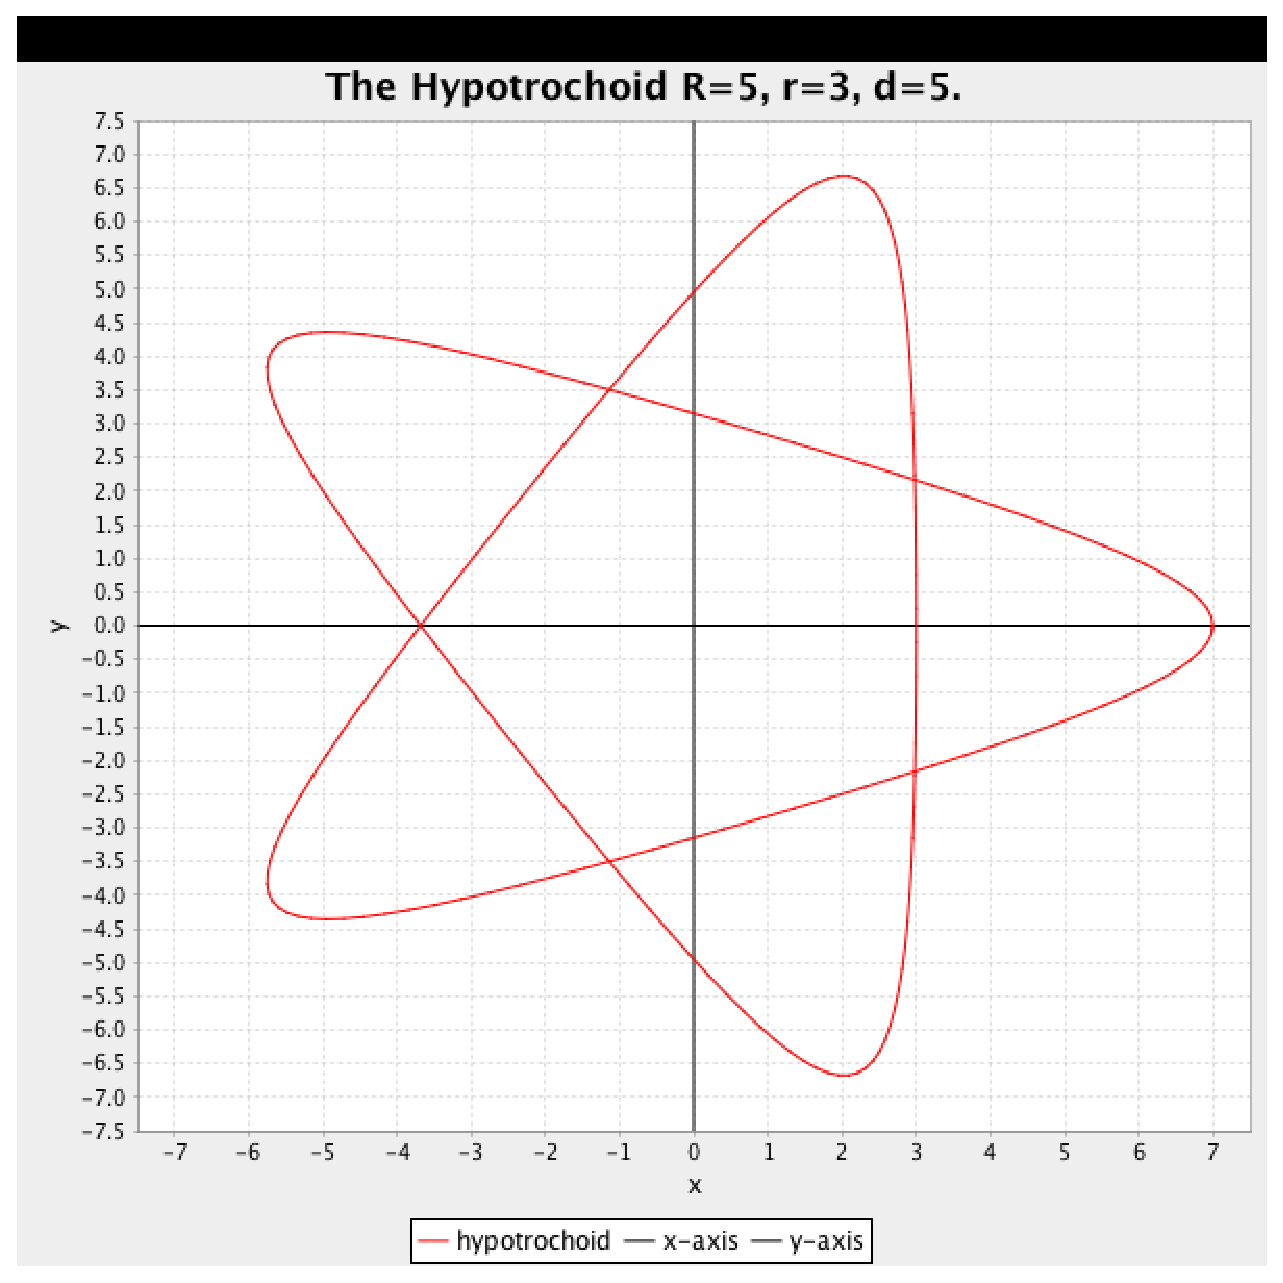
\epsfig{file=hypotrochoid.eps, scale=0.6}
  \caption{A plot of the hypotrochoid satisfying  $R = 5$, $r=3$, $d = 5$.}
  \label{fig:hypotrochoid.eps}
\end{figure}


\vspace*{\fill}
\pagebreak

\vspace*{\fill}
\pagebreak

\section{Scatter Plots}
In order to generate a \href{https://en.wikipedia.org/wiki/Scatter_plot}{scatter plot}, we can use
the function \texttt{plot\_addBullets}.  Figure \ref{fig:fathers-and-sons.stlx} on page
\pageref{fig:fathers-and-sons.stlx} shows the implementation of the function \texttt{fatherAndSons}
that reads a file containing the heights of fathers and their sons and that converts these data into
the scatter plot shown in Figure \ref{fig:fathers-and-sons.eps} on page
\pageref{fig:fathers-and-sons.eps}.  We proceed to discuss the details of the implementation of the
function \texttt{fatherAndSons}.
\begin{enumerate}
\item Line 2 reads the file ``\texttt{fathers-and-sons.txt}'' and converts this file into a list of
      strings that is called \texttt{data}.  Each string corresponds to one line in the file.
      The first line in the file has the form 
      \\[0.2cm]
      \hspace*{1.3cm}
      \texttt{65.04851 59.77827}
      \\[0.2cm]
      This line states that the first father-son pair in the data set consists of a father who is
      $65.04851$ inches tall, while his son is only $59.77827$ inches tall.\footnote{
        At this point you are probably wondering how it is possible that the height is measured with a
        precision of 5 digits.  Of course, when measuring body heights this is precision is not
        achievable.  The data set I am using here is part of
        the \href{http://www.r-project.org}{\texttt{R} project} and can be found in the package
        \\[0.2cm]
        \hspace*{1.3cm}
        \href{http://www.inside-r.org/packages/cran/UsingR/docs/father.son}{\texttt{UsingR}}
        \\[0.2cm]
        in the variable \texttt{father.son}. 
        My best guess is that the data set has suffered from some kind of unit conversion. 
      }.
\item Line 3 splits every string in the list \texttt{data} into a list of two strings.  These two
      strings are the strings representing the height of the father and the height of his son.
      Therefore, the variable \texttt{fsStr} is a list of pairs of strings.  These pairs correspond
      to the lines in the file ``\texttt{fathers-and-sons.txt}''.
\item Line 4 converts these strings into floating point values.  This is done using the conversion
      function \texttt{double} that takes a string and converts it into a floating point number.
\item Line 5 creates the canvas.
\item Line 6 takes the pairs  of floating point numbers and plots them as boxes of size $2.0$.
      Note that the size has to be specified as a floating point number:  Specifying the height as
      an integer will result in an error message.

      The function \texttt{plot\_addBullets} takes a list of pairs of the form $[x,y]$ where $x$
      specifies the $x$-coordinate and $y$ specifies the $y$-coordinate of a data point.  These data
      points are then plotted one by one.
\item As the heights vary between 58 inches and 80 inches, line 7 modifies the scale accordingly.
\item Line 8 modifies the size of the canvas so that the width and the height are the same.
\item Line 9 changes the labeling of the $x$-axis and of the $y$-axis using the function
      \texttt{plot\_labelAxis}.  This function takes three arguments.
      \begin{enumerate}
      \item The first  argument is the canvas.
      \item The second argument is the label of the $x$-axis.
      \item The third  argument is the label of the $y$-axis.
      \end{enumerate}
\item Line 10 saves the scatter plot into a file. The file is saved as a \texttt{.png} file.
\end{enumerate}



\begin{figure}[!ht]
\centering
\begin{Verbatim}[ frame         = lines, 
                  framesep      = 0.3cm, 
                  firstnumber   = 1,
                  labelposition = bottomline,
                  numbers       = left,
                  numbersep     = -0.2cm,
                  xleftmargin   = 0.0cm,
                  xrightmargin  = 0.0cm,
                ]
    fatherAndSons := procedure() {
        data  := readFile("fathers-and-sons.txt");
        fsStr := [ split(line, " "): line in data ];
        fs    := [ [double(x), double(y)] : [x,y] in fsStr ];
        c     := plot_createCanvas("Heights of Fathers vs. Heights of Sons.");
        plot_addBullets(c, fs, [0,0,255], 2.0);
        plot_modScale(c, [58, 80], [58, 80]);
        plot_modSize(c, [1000, 1000]);
        plot_labelAxis(c, "heights of fathers in inches", 
                          "heights of sons in inches"    );
        plot_exportCanvas(c, "fathers-and-sons");
    };
\end{Verbatim}
\vspace*{-0.3cm}
\caption{How to generate a scatter plot from data stored in a file.}
\label{fig:fathers-and-sons.stlx}
\end{figure}

\begin{figure}[!ht]
  \centering
  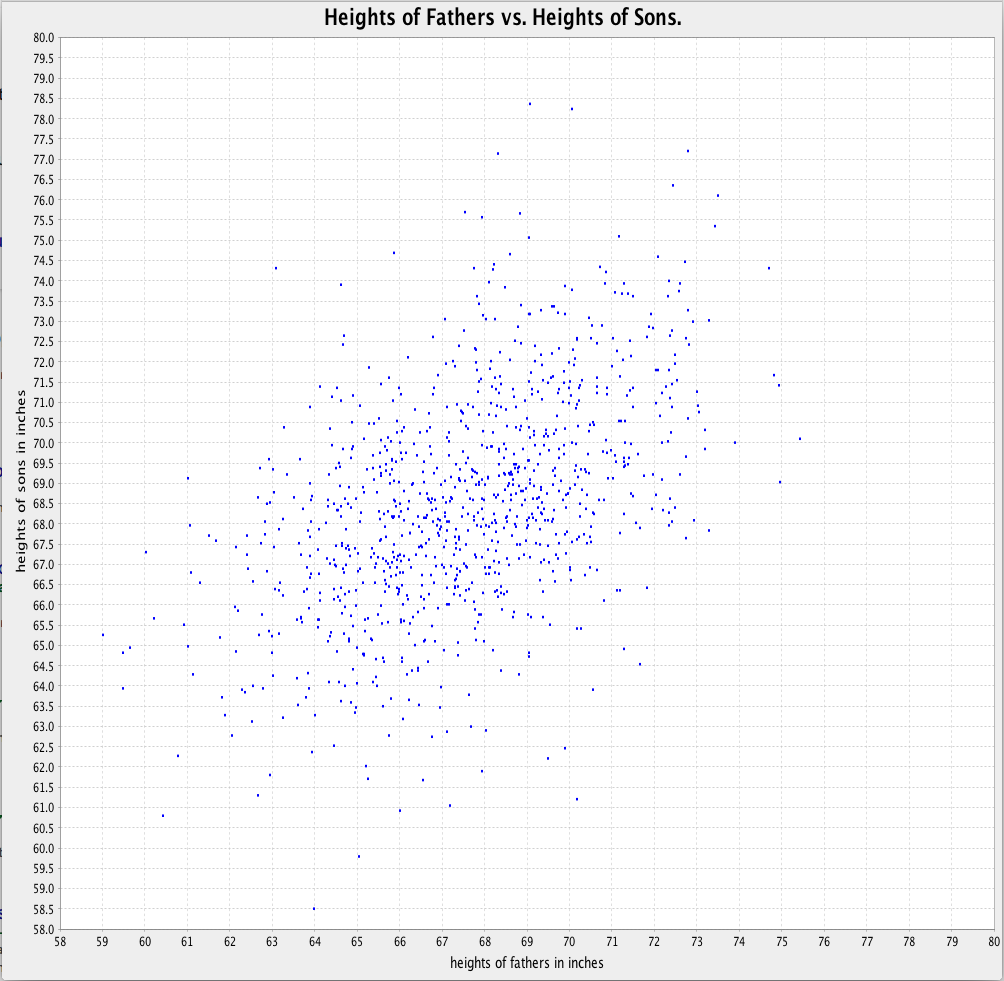
\epsfig{file=fathers-and-sons.eps, scale=0.4}
  \caption{A scatter plot showing the heights of fathers and their sons.}
  \label{fig:fathers-and-sons.eps}
\end{figure}

\vspace*{\fill}
\pagebreak


\section{Plotting Statistical Charts}
\setlx\ is able to draw \href{https://en.wikipedia.org/wiki/Bar_chart}{\emph{bar charts}} and
\href{https://en.wikipedia.org/wiki/Pie_chart}{\emph{pie charts}}.
We will present each of these charts in a separate subsection.

\subsection{Bar Charts}
\begin{table}
  \centering
  \begin{tabular}{|l|r|r|r|r|r|}
    \hline                                                     
    \diagbox{Region}{Year} & 1900 & 1950 & 1999 & 2008 & 2010 \\
    \hline                                                     
    \hline                                                     
    Northern America       &    82 &   172 &   307 &   337 &   345 \\
    \hline                                                      
    Oceania                &     6 &    13 &    30 &    34 &    37 \\
    \hline                                                     
    Latin America          &    74 &   167 &   511 &   577 &   590 \\
    \hline                                                     
    Europe                 &   408 &   547 &   729 &   732 &   738 \\ 
    \hline                                                     
    Africa                 &   133 &   221 &   767 &   973 & 1,022 \\ 
    \hline                                                     
    Asia                   &   947 & 1,402 & 3,634 & 4,054 & 4,164 \\
    \hline                                                     
    World                  & 1,650 & 2,521 & 5,978 & 6,707 & 6,896 \\
    \hline                                         
  \end{tabular}
  \caption{The world population in millions of people.}
  \label{tab:world-population}
\end{table}

\noindent
Table \ref{tab:world-population} on page \pageref{tab:world-population} shows the population of
different regions of the world for various years.  This data is more easily comprehensible when
presented as a bar char.  Figure \ref{fig:world-population.stlx} presents a \setlx-program that
converts these data into a bar chart.  We proceed to discuss this program line by line.
The bar chart produced by this program is shown in Figure \ref{fig:world-population.eps} on page
\pageref{fig:world-population.eps}.



\begin{figure}[!ht]
\centering
\begin{Verbatim}[ frame         = lines, 
                  framesep      = 0.3cm, 
                  firstnumber   = 1,
                  labelposition = bottomline,
                  numbers       = left,
                  numbersep     = -0.2cm,
                  xleftmargin   = 0.0cm,
                  xrightmargin  = 0.0cm,
                ]
    data := [ ["Year"            , 1900, 1950, 1999, 2008, 2010],
              ["Northern America",   82,  172,  307,  337,  345],
              ["Oceania"         ,    6,   13,   30,   34,   37],
              ["Latin America"   ,   74,  167,  511,  577,  590],
              ["Europe"          ,  408,  547,  729,  732,  738], 
              ["Africa"          ,  133,  221,  767,  973, 1022], 
              ["Asia"            ,  947, 1402, 3634, 4054, 4164],
              ["World"           , 1650, 2521, 5978, 6707, 6896] ];
    worldPopulation := procedure(data) {
        c       := plot_createCanvas();
        years   := data[1][2..];
        regions := [line[1]: line in data[2..]];
        for (i in [1..#years]) {
            population := [region[i+1] : region in data[2..]];
            plot_addBarChart(c, population, regions, "Population in $years[i]$");
        }
    };
    worldPopulation(data);
\end{Verbatim}
\vspace*{-0.3cm}
\caption{Program to plot the world population as a bar chart.}
\label{fig:world-population.stlx}
\end{figure}

\begin{enumerate}
\item Line 1 to line 8 define the data that is to be displayed.  The data is stored as a list of
      lists.  The first list specifies the years corresponding to the population counts.
      The remaining lists each specify the population counts for a specific geographical region.
\item The function \texttt{worldPopulation} has one parameter.  This parameter is of the form of the
      data specified in line 1 to line 8.
\item Line 10 creates the canvas.
\item Line 11 extracts the years.
\item Line 12 extract the regions from the first column of \texttt{data}.
\item Since our intention is to present the data of the different regions combined by the years, 
      we select these data in the list \texttt{population} in line 14.  Here, \texttt{region} iterates
      over the different regions in \texttt{data}, while \texttt{region[i+1]} selects the data for the $i$th
      year in the table.
\item The function \texttt{plot\_addBarChart} plots the bar chart. The arguments to this function 
      are as follows:
      \begin{enumerate}
      \item \texttt{c} specifies  the canvas.
      \item \texttt{population} is a list of numbers.  For every number in this list, the function 
            \texttt{plot\_addBarChart} plots a line of the corresponding height into each of the
            groups.  The groups are labeled by the list \texttt{regions}.  The lines plotted by one
            invocation of \texttt{plot\_addBarChart} all have the same unique color.  This color is
            determined automatically.
      \item \texttt{regions} is a list of strings specifying a label for each group.
      \item The last argument specifies a legend for the data plotted by this instance of 
            \texttt{plot\_addBarChart}.
      \end{enumerate}
\end{enumerate}
In order to understand what is plotted where, it is easiest to compare the variable \texttt{data} defined in Figure
\ref{fig:world-population.stlx} to the plot in Figure \ref{fig:world-population.eps}


\begin{figure}[!ht]
  \centering
  \epsfig{file=world-population.eps, scale=0.5}
  \caption{A Bar chart showing the world population in millions in different regions.}
  \label{fig:world-population.eps}
\end{figure}

\subsection{Pie Charts}
Table \ref{tab:race-prison} on Page \pageref{tab:race-prison} shows the distribution of
different races in the Texan population and in  the population of Texan prisons.  In order to
further our understanding of the data, let us visualize it via two pie charts.  The visualization is
achieved using the \setlx-program shown in Figure \ref{fig:race-and-incarceration.stlx} on page
\pageref{fig:race-and-incarceration.stlx}.  The resulting pie charts are shown in Figure 
\ref{fig:race-prison} on page \pageref{fig:race-prison}.  We proceed to discuss the \setlx-program.


\begin{table}[!hb]
  \centering
  \begin{tabular}{|l|r|r|}
    \hline
    Race  & Population & Prison Population \\
    \hline
    \hline
     white & 10933313 & 38396 \\
    \hline
    black  &  2404566 & 51649 \\
    \hline
    latino &  6669666 & 35028 \\
    \hline
    other  &   844275 &   582 \\
    \hline
  \end{tabular}
  \caption{The race distribution in the Texan population vs.~the Texan prison population.}
  \label{tab:race-prison}
\end{table}

\begin{figure}[!ht]
\centering
\begin{Verbatim}[ frame         = lines, 
                  framesep      = 0.3cm, 
                  firstnumber   = 1,
                  labelposition = bottomline,
                  numbers       = left,
                  numbersep     = -0.2cm,
                  xleftmargin   = 0.8cm,
                  xrightmargin  = 0.8cm,
                ]
    data := [ ["white", 10933313, 38396],
              ["black",  2404566, 51649],
              ["latino", 6669666, 35028],
              ["other",   844275,   582]
        ];
    prisonPopulation := procedure(data) {
        c1 := plot_createCanvas("Race disdribution in Texas.");
        c2 := plot_createCanvas("Race disdribution in Texan prisons.");
        races      := [line[1]: line in data];
        population := [line[2]: line in data];
        inmates    := [line[3]: line in data];
        plot_addPieChart(c1, population, races);
        plot_addPieChart(c2, inmates,    races);
        plot_exportCanvas(c1, "race-population");
        plot_exportCanvas(c2, "race-incarceration");
    };
\end{Verbatim}
\vspace*{-0.3cm}
\caption{A program to generate two pie charts.}
\label{fig:race-and-incarceration.stlx}
\end{figure}

\begin{enumerate}
\item The data are defined in line 1 to 5 as a list of list.  Each list in \texttt{data} corresponds
      to a different race. 
\item The procedure \texttt{prisonPopulation} takes this data as its sole input.
\item Line 7 and 8 create two different canvases for the two pie charts.
\item Line 9 extracts the different races stored in the table \texttt{data}.
\item Line 10 is defined as list containing the number of people of the various races living in
      Texas.
\item Line 11 is the corresponding list containing the number of prison inmates of each race.
\item Line 12 draws the pie chart showing the Texan race distribution via a call of the function
      \texttt{plot\_addPieChart}.
      \begin{enumerate}
      \item The first parameter specifies the canvas on which the pie chart is to be drawn.
      \item The second parameter is a list of numbers.
      \item The final parameter is a list of labels.
      \end{enumerate}
\item Line 13 draws the pie chart showing the  race distribution of Texan inmates.
\item The last two lines save the generated charts as \texttt{png} files.
\end{enumerate}

\begin{figure}[!ht]
  \centering
  \epsfig{file=race-population.eps, scale=0.6}
  \epsfig{file=race-incarceration.eps, scale=0.6}
  \caption{The race distribution in Texas and in Texan prisons.}
  \label{fig:race-prison}
\end{figure}



%%% Local Variables:
%%% mode: latex
%%% TeX-master: "tutorial.tex"
%%% End:

\chapter{Classes and Objects}
These days, everything is
\href{http://en.wikipedia.org/wiki/Object-oriented_programming}{\emph{object-oriented}}.  
After having spotted
\href{http://www.danielsen.com/jokes/objecttoaster.txt}{object-oriented toasters}  
on the loose, we have decided that \textsc{SetlX} should not be an exception.  Therefore,
\textsc{SetlX} supports some basic means for object-oriented programming.  Most importantly,
\textsc{SetlX} supports classes.  In \textsc{SetlX} a  
\href{http://en.wikipedia.org/wiki/Class_(computer_programming)}{\emph{class}}
is an agglomeration of variables and functions.  These variables are referred to as 
\emph{member variables}, while the functions are called \emph{methods}.  
In this chapter we demonstrate how classes can be defined and used in \textsc{SetlX}.  
However, this chapter is \underline{not} intended to be an introduction into object-oriented
programming.  Instead,  we assume that the reader 
has had some previous exposure to object-oriented programming via a programming language like \textsl{Java},
\texttt{C++}, or \textsl{Python}.  In the first section of this chapter, we give some simple
examples of class definitions.  
The programs presented in that section are not intended to compute anything useful.  Their
sole purpose is to demonstrate the basic features of object-oriented programming available
in \textsc{SetlX}.  The second  and third section will then discuss more interesting examples:
The second section shows how to implement weighted directed graphs via classes and the final
section discusses the implementation of complex numbers.  That section will also discuss
some of the more advanced features of object-oriented programming available in
\textsc{SetlX}.  In particular, we will discuss operator overloading.

\section{Basic Examples}
In this section, we introduce the basic means by which object-oriented programming is supported in
\textsc{SetlX}.  In the first subsection, we introduce classes.  The second subsection shows how to
simulate inheritance.

\subsection{Introducing Classes}
Our first example deals with the representation of points in a plane.  One way to specify a point
$p$ is to specify both its $x$ and its $y$-coordinate.  This leads to the class definition shown in
Figure \ref{fig:point.stlx} on page \pageref{fig:point.stlx}.  We discuss the details of this
definition next.

\begin{figure}[!ht]
\centering
\begin{Verbatim}[ frame         = lines, 
                  framesep      = 0.3cm, 
                  firstnumber   = 1,
                  labelposition = bottomline,
                  numbers       = left,
                  numbersep     = -0.2cm,
                  xleftmargin   = 0.8cm,
                  xrightmargin  = 0.8cm,
                ]
    class point(x, y) {
        mX := x;
        mY := y;
    
        getX  := procedure()  { return mX;             };
        getY  := procedure()  { return mY;             };
        setX  := procedure(x) { this.mX := x;          };
        setY  := procedure(y) { this.mY := y;          };
        toStr := procedure()  { return "<$mX$, $mY$>"; };

        distance := procedure(p) {
            return sqrt((mX - p.getX()) ** 2 + (mY - p.getY()) ** 2);
        };
    }
\end{Verbatim}
\vspace*{-0.3cm}
\caption{The class \texttt{point}.}
\label{fig:point.stlx}
\end{figure}

\begin{enumerate}
\item Line 1 defines the class \texttt{point} using the keyword \texttt{class}.  Note that
      line 1 simultaneously defines a constructor for this class.  This constructor takes two
      arguments \texttt{x} and \texttt{y}.  These two arguments are interpreted as the $x$ and
      $y$-coordinate of the point to construct.

      The general form of a class definition is as follows:
      \\[0.2cm]
      \hspace*{1.3cm}
      \texttt{class} \textsl{name}$(x_1, \cdots, x_n)$ \texttt{\{}  
      \\
      \hspace*{2.0cm} \textsl{member-and-method-definitions}
      \\
      \hspace*{1.3cm}
      \texttt{\}}
      \\[0.2cm]
      Here \textsl{name} is the name of the class that is defined, $x_1, \cdots, x_n$ are the formal
      parameters of the constructor of this class, and \textsl{member-and-method-definitions} is a
      list of the definitions of all member variables and methods.

      The definition of a class is \underline{not} terminated with the character ``\texttt{;}''.
      The reason is that, unlike most procedure definitions, a class definition is not part of an
      assignment.  Actually, a procedure definition does not contain an assignment either.  The
      reason that most procedure definitions are followed by a semicolon is the fact that most
      procedure definitions are part of an assignment.  In that case the semicolon following the procedure
      definition is syntactically not part of the procedure definition but rather terminates the assignment.
\item In line 2 and line 3 we define the member variables \texttt{mX} and \texttt{mY}.  These two
      member variables store the $x$ and $y$-coordinates of the point that is constructed.

      It is our convention to start member variables with a lower case letter ``\texttt{m}''.  This
      letter is intended as an abbreviation of \underline{m}ember.  The letter following the letter
      ``\texttt{m}'' will always be capitalized.  However, this convention is only our
      recommendation for naming member variables and you are free to choose any valid variable name
      to designate a member variable.
\item Line 5 to 8 define getter and setter methods to access and write the member variables
      \texttt{mX} and \texttt{mY}.  Note that, in order to \textbf{change} the value of a member variable, it
      is necessary to prefix this member variable with the keyword ``\texttt{this.}''.  However, this prefixing is not
      necessary in order to read a member variable, as can be seen in the implementation of the
      methods \texttt{getX} and \texttt{getY}.
\item Line 9 defines the method \texttt{toStr} that transforms a given object of class
      \texttt{point} into a string.
\item Finally, we define a method called \texttt{distance} that takes a point \texttt{p} as its
      argument.  This method computes the distance of the given point to the point \texttt{p}
      using the \href{http://en.wikipedia.org/wiki/Pythagorean_theorem}{Pythagorean theorem}.
\end{enumerate}
So far, we have only shown how to define a class but we have not yet seen how to use a class.
Therefore, assume that the code shown in Figure \ref{fig:point.stlx} has been loaded into the
interpreter.   Then we can define an object of class \texttt{point} by writing
\\[0.2cm]
\hspace*{1.3cm}
\texttt{origin := point(0, 0);}
\\[0.2cm]
and the statement
\\[0.2cm]
\hspace*{1.3cm}
\texttt{print(origin.toStr());}
\\[0.2cm] 
would result in the following output:
\\[0.2cm]
\hspace*{1.3cm}
\texttt{<0, 0>}
\\[0.2cm]
It is instructive to print the object \texttt{origin} itself.  The statement 
\\[0.2cm]
\hspace*{1.3cm}
\texttt{print(origin);}
\\[0.2cm]
yields the output that is shown in Figure \ref{fig:print_origin} on page \pageref{fig:print_origin}.
Note that we have formatted this output in order to render it more readable.  Closer inspection of the
output reveals that an object is just a collection of all its members.  As \textsc{SetlX} is a functional
language, there is really no distinction between a member variable and a method.  For example, in
line 5 the variable \texttt{toStr} is just a member variable which happens to be bound to a
procedure.  Note that the object \texttt{origin} also has a method \texttt{getClass}.
The definition of this method is shown in line 12 -- 23.  This
method is generated automatically for every class that is defined.  Technically,
this method returns the class definition.  Practically , this method can used
to check whether two objects have the same class.  For example, after defining 
\\[0.2cm]
\hspace*{1.3cm} \texttt{p1 := point(1, 2);} \\
\hspace*{1.3cm} \texttt{p2 := point(2, 1);} 
\\[0.2cm]
\texttt{p1} and \texttt{p2} are different objects but the test
\\[0.2cm]
\hspace*{1.3cm}
\texttt{p1.getClass() == p2.getClass()}
\\[0.2cm]
will return \texttt{true}.  If we only are interested whether the object \texttt{p1} is of class
\texttt{point} we can write the test as
\\[0.2cm]
\hspace*{1.3cm}
\texttt{p1.getClass() == point}.
\\[0.2cm]
This works, since after defining the class \texttt{point}, the variable \texttt{point} is bound to
the class object shown in Figure \ref{fig:point-class} on page \pageref{fig:point-class}.

\begin{figure}[!ht]
\centering
\begin{Verbatim}[ frame         = lines, 
                  framesep      = 0.3cm, 
                  firstnumber   = 1,
                  labelposition = bottomline,
                  numbers       = left,
                  numbersep     = -0.2cm,
                  xleftmargin   = 0.0cm,
                  xrightmargin  = 0.0cm,
                ]
    object<
        { distance := procedure(p) { 
                          return sqrt((mX - p.getX()) ** 2 + (mY - p.getY()) ** 2); 
                      }; 
          getX := procedure() { return mX; }; 
          getY := procedure() { return mY; }; 
          mX := 0; 
          mY := 0; 
          setX := procedure(x) { this.mX := x; }; 
          setY := procedure(y) { this.mY := y; }; 
          toStr := procedure() { return "<$mX$, $mY$>"; }; 
          getClass := [] |-> class (x, y) { 
              mX := x; 
              mY := y; 
              distance := procedure(p) { 
                  return sqrt((mX - p.getX()) ** 2 + (mY - p.getY()) ** 2); 
              }; 
              getX := procedure() { return mX; }; 
              getY := procedure() { return mY; }; 
              setX := procedure(x) { this.mX := x; }; 
              setY := procedure(y) { this.mY := y; }; 
              toStr := procedure() { return "<$mX$, $mY$>"; }; 
          }
        }
    >
\end{Verbatim}
\vspace*{-0.3cm}
\caption{The output of the command ``\texttt{print(origin);}''.}
\label{fig:print_origin}
\end{figure}

\begin{figure}[!ht]
\centering
\begin{Verbatim}[ frame         = lines, 
                  framesep      = 0.3cm, 
                  firstnumber   = 1,
                  labelposition = bottomline,
                  numbers       = left,
                  numbersep     = -0.2cm,
                  xleftmargin   = 0.0cm,
                  xrightmargin  = 0.0cm,
                ]
    class (x, y) { 
        mX := x; 
        mY := y; 
        distance := procedure(p) { 
            return sqrt((mX - p.getX()) ** 2 + (mY - p.getY()) ** 2); 
        }; 
        getX := procedure() { return mX; }; 
        getY := procedure() { return mY; }; 
        setX := procedure(x) { this.mX := x; }; 
        setY := procedure(y) { this.mY := y; }; 
        toStr := procedure() { return "<$mX$, $mY$>"; }; 
    }
\end{Verbatim}
\vspace*{-0.3cm}
\caption{The class object corresponding to the class \texttt{point}.}
\label{fig:point-class}
\end{figure}

At first, the fact that all methods are stored as part of the object \texttt{origin} might seem quite
wasteful.  However, this fact enables us to change these methods dynamically.  For example, we can
realize that the $x$ and $y$-coordinates of the particular object \texttt{origin} really are fixed.
Therefore, the getter methods can be 
simplified and the setter methods can even be eliminated.  Assuming \texttt{origin} is defined as
\\[0.2cm]
\hspace*{1.3cm}
\texttt{origin := point(0, 0);}
\\[0.2cm]
we could then write the code shown in Figure \ref{fig:point.stlx-origin}.
This code would make it impossible to call the setter methods for the object \texttt{origin}.

\begin{figure}[!ht]
\centering
\begin{Verbatim}[ frame         = lines, 
                  framesep      = 0.3cm, 
                  firstnumber   = 1,
                  labelposition = bottomline,
                  numbers       = left,
                  numbersep     = -0.2cm,
                  xleftmargin   = 0.8cm,
                  xrightmargin  = 0.8cm,
                ]
    origin.getX := procedure() { return 0; };
    origin.getY := procedure() { return 0; };
    origin.setX := om;
    origin.setY := om;
\end{Verbatim}
\vspace*{-0.3cm}
\caption{Changing the methods attached to \texttt{origin}.}
\label{fig:point.stlx-origin}
\end{figure}

\begin{figure}[!htb]
\centering
\begin{Verbatim}[ frame         = lines, 
                  framesep      = 0.3cm, 
                  firstnumber   = 1,
                  labelposition = bottomline,
                  numbers       = left,
                  numbersep     = -0.2cm,
                  xleftmargin   = 0.8cm,
                  xrightmargin  = 0.8cm,
                ]
    class point(x, y) {
        mX := x;
        mY := y;
    
      static {
        getX  := procedure()  { return mX;             };
        getY  := procedure()  { return mY;             };
        setX  := procedure(x) { this.mX := x;          };
        setY  := procedure(y) { this.mY := y;          };
        toStr := procedure()  { return "<$mX$, $mY$>"; };
 
        distance := procedure(p) {
            return sqrt((mX - p.getX()) ** 2 + (mY - p.getY()) ** 2);
        };
      }
    }
\end{Verbatim}
\vspace*{-0.3cm}
\caption{The class \texttt{point} implemented using static methods.}
\label{fig:point-static.stlx}
\end{figure}

On the other hand, if we choose not to change methods on a per-object basis, we could just as well
declare these methods to be static.  Then, the resulting code would look as shown in Figure
\ref{fig:point-static.stlx} on page \pageref{fig:point-static.stlx}.  The only difference to our
first implementation of the class \texttt{point} shown in Figure \ref{fig:point.stlx} on page
\pageref{fig:point.stlx} is the \texttt{static} block that starts in line 5 and ends in line 15.
If we now define \texttt{origin} as
\\[0.2cm]
\hspace*{1.3cm}
\texttt{origin := point(0, 0);}
\\[0.2cm]
and print \texttt{origin}, then the resulting output would be as shown in Figure
\ref{fig:point-static.stlx-origin} on page \pageref{fig:point-static.stlx-origin}.
Note that in this case only the member variables are stored in the object
\texttt{origin}.  This saves some space.  
Fortunately, we can still overwrite the static methods on a per-object
basis, i.e.~the assignments
\begin{verbatim}
    origin.getX := procedure() { return 0; };
    origin.getY := procedure() { return 0; };
    origin.setX := om;
    origin.setY := om;
\end{verbatim}
will create member variables \texttt{getX}, \texttt{getY}, \texttt{setX}, and \texttt{setY}
that are attributes of the object \texttt{origin}.  The static variables of the same name are
unchanged but an expression of the form
\\[0.2cm]
\hspace*{1.3cm}
\texttt{origin.getX()}
\\[0.2cm]
invokes the function bound to the member variable \texttt{getX} and does no longer invoke
the function bound to the static variable \texttt{getX}.  Hence, the static member functions are
effectively hidden.

Going back to the code in Figure \ref{fig:point-static.stlx}, note that in order to invoke one of these
static methods we still need an object of class \texttt{point}.  The reason is that otherwise the
variables \texttt{mX} and \texttt{mY}, which are used in these methods, would be undefined.

\begin{figure}[!ht]
\centering
\begin{Verbatim}[ frame         = lines, 
                  framesep      = 0.3cm, 
                  firstnumber   = 1,
                  labelposition = bottomline,
                  numbers       = left,
                  numbersep     = -0.2cm,
                  xleftmargin   = 0.0cm,
                  xrightmargin  = 0.0cm,
                ]
    object<
        { mX := 0; 
          mY := 0; 
          getClass := [] |-> class (x, y) { 
              mX := x; 
              mY := y; 
            static { 
              distance := procedure(p) { 
                  return sqrt((mX - p.getX()) ** 2 + (mY - p.getY()) ** 2); 
              }; 
              getX := procedure() { return mX; }; 
              getY := procedure() { return mY; }; 
              setX := procedure(x) { this.mX := x; }; 
              setY := procedure(y) { this.mY := y; }; 
              toStr := procedure() { return "<$mX$, $mY$>"; }; 
            } 
          }
        }
    >
\end{Verbatim}
\vspace*{-0.3cm}
\caption{Output of ``\texttt{print(origin);}''.}
\label{fig:point-static.stlx-origin}
\end{figure}

The last remark might confuse people accustomed to a programming language like \textsl{Java}.  Let
us therefore elaborate: If we use the definition of the class \texttt{point} shown in Figure
\ref{fig:point-static.stlx} on page \pageref{fig:point-static.stlx} and define the object
\texttt{origin} as
\\[0.2cm]
\hspace*{1.3cm}
\texttt{origin := point(0,0);}
\\[0.2cm]
then we can issue the command
\\[0.2cm]
\hspace*{1.3cm}
\texttt{print(point.getX);}
\\[0.2cm]
and get the result
\\[0.2cm]
\hspace*{1.3cm}
\texttt{procedure() \{ return mX; \}}.
\\[0.2cm]
This shows that the method \texttt{getX} is indeed a property of the class \texttt{point}.  However, 
we cannot invoke this method on the class \texttt{point} because this method needs access to the
member variable \texttt{mX} and this member variable is only available in objects of class
\texttt{point}, but it is not an attribute of the class \texttt{point} itself, since only members
defined as \texttt{static} are attributes of a class.  Therefore, the command
\\[0.2cm]
\hspace*{1.3cm}
\texttt{point.getX();}
\\[0.2cm]
yields the output
\\[0.2cm]
\hspace*{1.3cm}
\texttt{\~{}< Result: om >\~}
\\[0.2cm]
indicating that \texttt{mX} is undefined.  

Of course, classes can have static variables.  These are
then accessible by means  of the class name.  This way, we can simulate global variables in
\textsc{SetlX}.  For example, we can define the class \texttt{universal} as shown in Figure
\ref{fig:universal.stlx}.  Then, we can always access the 
\href{http://en.wikipedia.org/wiki/Answer_to_the_Ultimate_Question_of_Life,_the_Universe,_and_Everything#Answer_to_the_Ultimate_Question_of_Life.2C_the_Universe_and_Everything_.2842.29}{universal constant}
 using the expression
\\[0.2cm]
\hspace*{1.3cm}
\texttt{universal.sAnswer}
\\[0.2cm]
Note that we can both read and write to this variable.  We have started the name of the variable
``\texttt{sAnswer}'' with a lower case ``\texttt{s}'' since this is our naming convention for static variables.
\begin{figure}[!ht]
\centering
\begin{Verbatim}[ frame         = lines, 
                  framesep      = 0.3cm, 
                  firstnumber   = 1,
                  labelposition = bottomline,
                  numbers       = left,
                  numbersep     = -0.2cm,
                  xleftmargin   = 0.8cm,
                  xrightmargin  = 0.8cm,
                ]
    class universal() {
      static {
        sAnswer := 42;
      }
    }
\end{Verbatim}
\vspace*{-0.3cm}
\caption{Defining global variables as static members of a class.}
\label{fig:universal.stlx}
\end{figure}



\subsection{Simulating Inheritance}
Continuing the example of the class \texttt{point} shown in Figure \ref{fig:point.stlx}, let us
assume that some points have a color as an additional attribute.  If we were programming in
\textsl{Java} and wanted to support both points with and without a color, we could create a class
\texttt{coloredPoint} that extends the class \texttt{point}.  The mechanics are a little different
in \textsc{SetlX}.  Figure \ref{fig:point-colored.stlx} on page \pageref{fig:point-colored.stlx}
shows how to implement both ordinary points and colored points in \textsc{SetlX}.

\begin{figure}[!ht]
\centering
\begin{Verbatim}[ frame         = lines, 
                  framesep      = 0.3cm, 
                  firstnumber   = 1,
                  labelposition = bottomline,
                  numbers       = left,
                  numbersep     = -0.2cm,
                  xleftmargin   = 0.8cm,
                  xrightmargin  = 0.8cm,
                ]
    class point(x, y) {
        mX := x;
        mY := y;
    
        getX  := procedure()  { return mX;             };
        getY  := procedure()  { return mY;             };
        setX  := procedure(x) { this.mX := x;          };
        setY  := procedure(y) { this.mY := y;          };
        toStr := procedure()  { return "<$mX$, $mY$>"; };
        distance := procedure(p) {
            return sqrt((mX - p.getX()) ** 2 + (mY - p.getY()) ** 2);
        };
    }
    class color(r, g, b) {
        mR := r; mG := g; mB := b;
    }    
    coloredPoint := procedure(x, y, c) {
        p := point(x, y);
        p.mColor := c;
        
        p.toStr := procedure() {
            return "<$mX$, $mY$>: $mColor.mR$, $mColor.mG$, $mColor.mB$";
        };
        return p;
    };
\end{Verbatim}
\vspace*{-0.3cm}
\caption{Representing colored points.}
\label{fig:point-colored.stlx}
\end{figure}

\begin{enumerate}
\item Line 1 defines the class \texttt{point}.  The definition is the same as in Figure
     \ref{fig:point.stlx}.
\item Line 14 defines the class \texttt{color}.  This class stored the color by its 
      \href{http://en.wikipedia.org/wiki/RGB_color_model}{rgb} value: The member variable
      \texttt{mR} specifies the luminosity of the red color component, \texttt{mG} gives the 
      luminosity of the green color component, and \texttt{mB} defines the blue color component.

      Note that it is not necessary to implement getters and setters for these member variables since
      in \textsc{SetlX} all member variables are accessible in the methods of the class.
\item Line 17 defines the procedure \texttt{coloredPoint}.  This procedure takes three arguments:
      \begin{enumerate}
      \item $x$ and $y$ specify the $x$ and $y$-coordinate of the given point and
      \item $c$ specifies the color of the point.
      \end{enumerate}
      The procedure \texttt{coloredPoint} constructs a colored point.  In order to do so, it takes 
      the following steps:
      \begin{enumerate}
      \item Line 18 creates an ordinary \texttt{point} $p$ that has the specified coordinates.
      \item Line 19 adds the member variable \texttt{mColor} to the \texttt{point} $p$.

            Note that in \textsc{SetlX} it is possible to add member variables dynamically to a given object.
      \item Line 21 changes the method \texttt{toStr} for the object $p$.  The new implementation
            return both the coordinates and the color information.
      \item Finally, the object $p$ is returned.
      \end{enumerate}
      Note that the procedure \texttt{coloredPoint} is effectively a constructor for objects
      that have class \texttt{point} but also have a color attribute.  It could be called a
      \href{http://en.wikipedia.org/wiki/Factory_method_pattern}{\emph{factory method}}.
\end{enumerate}



\section{A Case Study: Dijkstra's Algorithm}
In this section we show how to represent a weighted
directed graph $G = \langle V, E, \mathtt{length} \rangle$ as a class.  Here, $V$ is the
set of nodes, $E$ is the set of edges, where an edge is a pair of nodes, and 
\\[0.2cm]
\hspace*{1.3cm}
$\texttt{length}: E \rightarrow \mathbb{N}$
\\[0.2cm]
is a function assigning a \emph{length} to every edge.  We will present 
\href{http://en.wikipedia.org/wiki/Dijkstra%27s_algorithm}{Dijkstra's algorithm} 
for computing distances in a weighted directed graph.
Figure \ref{fig:graph.eps} on page \pageref{fig:graph.eps} shows a weighted directed graph.  The set
of nodes $V$ of this graph is given as 
\\[0.2cm]
\hspace*{1.3cm}
$V = \{1,2,3,4,5\}$,
\\[0.2cm] 
the set of edges is 
\\[0.2cm]
\hspace*{1.3cm}
$E = \{ \pair(1,5), \pair(1,3), \pair(5,2), \pair(3,2), \pair(2,4), \pair(3,4) \}$,
\\[0.2cm]
and the function $\mathtt{length}$ is given as the relation
\\[0.2cm]
\hspace*{1.3cm}
$\mathtt{length} = \bigl\{\, \bigl\langle\pair(1,5), 3 \bigr\rangle,\,
                             \bigl\langle\pair(1,3), 5 \bigr\rangle,\,
                             \bigl\langle\pair(5,2), 1 \bigr\rangle,\,
                             \bigl\langle\pair(3,2), 2 \bigr\rangle,\,
                             \bigl\langle\pair(2,4), 4 \bigr\rangle,\,
                             \bigl\langle\pair(3,4), 7 \bigr\rangle\,
                   \bigr\}$.
\\[0.2cm]
For example, $\mathtt{length}(\pair(1,5)) = 3$ and $\mathtt{length}(\pair(1,3)) = 5$.
In this graph, the shortest path from the node 1 to the node 4 is
given by the list $[1,5,2,4]$ and therefore the distance between these
nodes is $3 + 1 + 4 = 8$.

\begin{figure}[!ht]
  \centering
  \framebox{\epsfig{file=graph.eps, scale=0.7}} 
  \caption{A simple weighted directed graph.}
  \label{fig:graph.eps}
\end{figure}


In order to compute the distances from a given node to all other nodes we first have to decide how
to represent a weighted directed graph.  In our implementation of Dijkstra's algorithm we will
assume that the set of nodes $V$ is given as a set of consecutive natural numbers of the form
\\[0.2cm]
\hspace*{1.3cm}
$V = \{ 1, 2, \cdots, n-1, n \}$.
\\[0.2cm]
Therefore, there is no need to store the set $V$.  All we have to store is the number of nodes $n$.
The set of edges $E$ and the function \texttt{length} will be stored using (a variant of) an
\href{http://en.wikipedia.org/wiki/Adjacency_list}{\emph{adjacency list representation}}.
To this end, we define a binary relation \texttt{edges} so that for every node $x \in V$ the
expression \texttt{edges[$x$]} is a set of the form
\\[0.2cm]
\hspace*{1.3cm}
$\texttt{edges[}x\mathtt{]} = \{ [y_1,w_1], \cdots [y_n,w_n] \}$, 
\\[0.2cm]
so that there is an edge form $x$ to $y_i$ for all $i=1,\cdots,n$ and, furthermore, the length of
this edge is $w_i$, i.e.~we have 
\\[0.2cm]
\hspace*{1.3cm}
$\mathtt{length}([x,y_i]) = w_i$ \quad for all $i=1,\cdots,n$.
\\[0.2cm]
Stated differently, if $x$ and $y$ are nodes in $V$ such that $\pair(x,y)$ is an edge in $E$ of length
$w$, then we have
\\[0.2cm]
\hspace*{1.3cm}
$[y,w] \in \mathtt{edges[}x\mathtt{]}$.
\\[0.2cm]
For example, the relation \texttt{edges} for the graph shown in Figure \ref{fig:graph.eps} can be
defined in \textsc{SetlX} as follows:
\\[0.2cm]
\hspace*{1.3cm}  \texttt{edges := \{ [1, \{[5,3]], [3,5]\}], \\
\hspace*{3.25cm}                     [5, \{[2,1]\}],         \\
\hspace*{3.25cm}                     [3, \{[2,2], [4,7]\}],  \\
\hspace*{3.25cm}                     [2, \{[4,4]\}],         \\
\hspace*{3.25cm}                     [4, \{\}]               \\
\hspace*{2.9cm}                  \};}


\begin{figure}[!ht]
\centering
\begin{Verbatim}[ frame         = lines, 
                  framesep      = 0.3cm, 
                  firstnumber   = 1,
                  labelposition = bottomline,
                  numbers       = left,
                  numbersep     = -0.2cm,
                  xleftmargin   = 0.8cm,
                  xrightmargin  = 0.8cm,
                ]
    class graph(numberNodes, edges) {
        mNumberNodes := numberNodes;
        mEdges       := edges;
    
      static {
        shortestPath := procedure(source) {
            oo   := mathConst("Infinity");
            dist := { [x, oo]: x in [1 .. mNumberNodes] };
            dist[source] := 0;
            fringe  := { [0, source] };
            visited := {};
            while (fringe != {}) {
                [d, u] := first(fringe);
                fringe -= { [d, u] };
                for ([v,l] in mEdges[u] | !(v in visited)) {
                    if (d + l < dist[v]) {
                        dvOld := dist[v];
                        dvNew := d + l;
                        dist[v] := dvNew;
                        fringe -= { [dvOld, v] };
                    }
                    fringe += { [dist[v], v] };
                }
                visited += { u };
            }
            return dist;
        };
      }
    }
\end{Verbatim}
\vspace*{-0.3cm}
\caption{A class to represent graphs with an implementation of Dijkstra's algorithm.}
\label{fig:dijkstra.stlx}
\end{figure}

\vspace*{0.3cm}

\noindent
Now we are ready to present Dijkstra's algorithm in \textsc{SetlX}.
Figure \ref{fig:dijkstra.stlx} on page \pageref{fig:dijkstra.stlx} shows the implementation of the
class \texttt{graph} that is used to represent a weighted directed graph.  We discuss the
implementation line by line.
\begin{enumerate}
\item Line 1 starts to define the class \texttt{graph} and the constructor for
      this class.  In \textsc{SetlX}, every class has exactly one constructor and the definition of
      the class and the constructor are the same.  

      In this case, the constructor takes two arguments.  
      \begin{enumerate}
      \item The first argument \texttt{numberNodes}
            specifies the number of nodes.  Implicitly, this argument also specifies the set of nodes
            of the graph since we have agreed that the set of nodes $V$ has the form
            \\[0.2cm]
            \hspace*{1.3cm}
            $V = \{1,2,\cdots, n-1, n\}$.
            \\[0.2cm]
            Therefore, since \texttt{numberNodes} is the number of nodes, we must have 
            $n = \mathtt{numberNodes}$.
      \item The second argument \texttt{edges} specifies both the set of edges and the function
            \texttt{length}  in the way discussed above.
      \end{enumerate}
\item Line 2 and 3 define and assign the member variables \texttt{mNumberNodes} and \texttt{mEdges}.
      Every object $o$ of class \texttt{graph} will therefore have the two attributes
      \texttt{mNumberNodes} and \texttt{mEdges}.  For a given object $o$, these attributes can be
      accessed as $o\mathtt{.mNumberNodes}$ and $o\mathtt{.mEdges}$ respectively.  
      These variables store the number of nodes and the edges in the way discussed previously.
\item Line 5 declares the beginning of a static block which ends in line 28.  
      In this case, the static block contains only the definition of the variable \texttt{shortestPath}.
      Of course, if $o$ is an object of class
      \texttt{graph} then $o\mathtt{.shortestPath}$ will access the function stored in the
      static variable \texttt{shortestPath}.  We defer the discussion of the implementation of this
      function.
\end{enumerate}
At this point, it should be noted that the function \texttt{shortestPath} accesses the variables
\texttt{mNumberNodes} and \texttt{mEdges} 
and these variables are \underline{not} static.  The reason the function \texttt{shortestPath} is
defined \texttt{static} is the fact that the implementation of this function is always the same, no
matter what the graph is.  Therefore, 
there is no need to store this implementation on a per object basis.  Hence, it is sufficient to provide this
function as a static variable of the class \texttt{graph}.  Of course, calling this function as
\\[0.2cm]
\hspace*{1.3cm}
$\texttt{graph.shortestPath}(s)$
\\[0.2cm]
wouldn't make any sense as then the variables \texttt{mNumberNodes} and \texttt{mEdges} would both
be undefined.  In order to call this function, we need to have an object $g$ of class \texttt{graph}.
Then it is possible to write
\\[0.2cm]
\hspace*{1.3cm}
$g\mathtt{.shortestPath}(s)$
\\[0.2cm]
as in this case the function \texttt{shortestPath} has access to the member variables
\texttt{mNumberNodes} and \texttt{mEdges} that are stored in the object $g$.

Let us now briefly explain the implementation of the function \texttt{shortestPath}.  This function
gets a single node \texttt{source} as its argument and it will compute the distance of all other
nodes from the node \texttt{source}.  This distance will be represented as a binary relation that is stored
in the variable \texttt{dist}.  The elements of this binary relation will be pairs of the form
\\[0.2cm]
\hspace*{1.3cm}
$[x, d]$
\\[0.2cm]
where $x$ is a node and $d$ is the distance of this node.
When given the graph $g$ depicted in Figure \ref{fig:dijkstra.stlx}, the
expression 
\\[0.2cm]
\hspace*{1.3cm}
$g\mathtt{.shortestPath(1)}$
\\[0.2cm]
will yield the result
\\[0.2cm]
\hspace*{1.3cm}
\texttt{\{[1, 0], [2, 4], [3, 5], [5, 3], [4, 8]\}}.
\\[0.2cm]
This elements of this binary relation are to be interpreted as follows:  
\begin{enumerate}
\item The distance of the node $1$ from the node $1$ is obviously $0$.
\item The distance of the node $2$ from the node $1$ is $4$.  
      The path $[1,5,2]$ exhibits this length.
\item $\vdots$
\item The distance of the node $4$ from the node $1$ is $8$.
      The path $[1,5,2,4]$ is the shortest path connecting the node $1$ with the node $4$
      and has length $8$.
\end{enumerate}
The relation \texttt{dist}, which is computed and returned by the function \texttt{shortestPath}, is
initialized in line 8 to assign the distance $\infty$ for every node $x$ of the graph.  This distance
can be seen as an upper estimate of the minimum length of a path connecting the \texttt{source} to
the node $x$.  Since we do not yet know whether the node $x$ is reachable from the node
\texttt{source} at all, we initialize the distance to $\infty$.
Initially, the only node that is definitely reachable from the node \texttt{source} is the node
\texttt{source} itself.  Therefore, \texttt{dist[source]} is set to $0$ in line 9.

The algorithm to compute all distances maintains two data structures.
\begin{enumerate}
\item \texttt{fringe} is the set of those nodes $x$ that have already been encountered when traversing
      the graph, but which have not been fully explored in the sense that there might exist nodes $y$ such
      that there is an edge $\pair(x,y)$ and the node $y$ has not been visited.
      
      However, instead of just storing these nodes, for every node $y$ the set \texttt{fringe} stores a pair
      of the form 
      \\[0.2cm]
      \hspace*{1.3cm}
      $[w, y]$,
      \\[0.2cm]
      where $w$ is the best estimate of the distance of the node $y$ from the node \texttt{source}.
      Initially, we have only visited the node \texttt{source} and its distance from \texttt{source}
      is obviously $0$.  Therefore, \texttt{fringe} is initialized as
      \\[0.2cm]
      \hspace*{1.3cm}
      \texttt{\{ [0, source] \}}
      \\[0.2cm]
      in line 13.  Since a node $u$ with distance $d$ is stored as the pair $[d, u]$, the set
      \texttt{fringe} can be used as a \href{https://en.wikipedia.org/wiki/Priority_queue}{priority queue}.  
      The reason is that in \textsc{SetlX} every 
      set is stored as an ordered binary tree.  Therefore, the elements of a set are ordered and it
      is easy to pick the smallest element of a set using the function \texttt{first}.  
      Since, furthermore, lists (and pairs in
      particular) are ordered lexicographically, the first element in the set \texttt{fringe} is 
      the pair $[d, u]$ with the smallest value of $d$, i.e.~the node $u$ in the set \texttt{fringe}
      that is closest to the \texttt{source}.
\item \texttt{visited} is the set of nodes that have been \emph{visited} in the following sense:
      A node $x$ is said to have been \emph{visited} if all of the neighbours of $x$, i.e.~all nodes
      $y$ such that there is an edge $\pair(x,y)$ have been inspected and have been assigned a 
      distance.  It may be the case that the distance assigned to $y$ will improve later,
      but once a node $x$ is added to the set \texttt{visited}, the distance of $x$ from
      \texttt{source} is known.  Initially, the set \texttt{visited} is empty.
\end{enumerate}
The workhorse of the function \texttt{shortestPath} is the \texttt{while}-loop in line 12.  As long
as there are nodes $u$ in the \texttt{fringe} we try to improve the estimate $\mathtt{dist}[v]$ for
all nodes $v$ such that there is an edge $\pair(u,v)$ from $u$ to $v$.  The idea is that if 
\\[0.2cm]
\hspace*{1.3cm}
$\mathtt{dist}[u] + l < \mathtt{dist}[v]$, \quad where $l$ is the length of the edge $\pair(u,v)$
\\[0.2cm]
then we can improve our estimate of $\texttt{dist}[v]$ by assigning
\\[0.2cm]
\hspace*{1.3cm}
\texttt{dist[v] := dist[u] + l;}
\\[0.2cm]
After updating the distance of node $v$, we have to add this node to the \texttt{fringe} so that we
can in turn deal with those nodes that are reachable from node $v$.  The thing that makes Dijkstra's
algorithm fast is the fact that once a node is visited it can be shown that its distance can not be
improved further.  A proof of this fact can be found in a 
\href{http://www-m3.ma.tum.de/foswiki/pub/MN0506/WebHome/dijkstra.pdf}{paper} of Dijkstra \cite{dijkstra:59}.
\vspace*{0.3cm}

\noindent
\textbf{Remark}:  At this point you might feel a little bit disappointed because the previous example
has not made much use of the object-oriented features of \textsc{SetlX}.  However, that is exactly
the point of this example: Of course we could have implemented graph nodes as object of some class
and do the same for edges.  However, the resulting program would then suffer from 
\href{https://en.wikipedia.org/wiki/Code_bloat}{code bloat}.  We do
not think that object-oriented programming should be used for the sake of object-oriented
programming but rather see it as a convenient method to encapsulate data, nothing more.  In
particular, an object-oriented program is not, in general, better than a program that does not use
object-oriented features.  We therefore advocate to use classes when this is either necessary or 
convenient but not for the sake of object-oriented programming.

\section{Representing Complex Numbers as Objects}
Our next example deals with 
\href{http://en.wikipedia.org/wiki/Complex_number}{\emph{complex numbers}}.  
Remember that complex numbers have the form
\\[0.2cm]
\hspace*{1.3cm}
$z = x + y \cdot i$, \quad where $x,y \in \mathbb{R}$ and $i \cdot i = -1$.
\\[0.2cm]
Assume that we have to perform a number of intricate calculations using complex numbers.  One way
we could do this is by representing a complex number $x + y \cdot i$ as a pair $[x,y]$.  Then we
would have to implement functions to add, subtract, multiply,  and divide complex numbers.  For
example, methods to add and multiply two complex numbers would have the form shown in Figure
\ref{fig:add-complex.stlx} on page \pageref{fig:add-complex.stlx}.
 

\begin{figure}[!ht]
\centering
\begin{Verbatim}[ frame         = lines, 
                  framesep      = 0.3cm, 
                  firstnumber   = 1,
                  labelposition = bottomline,
                  numbers       = left,
                  numbersep     = -0.2cm,
                  xleftmargin   = 0.8cm,
                  xrightmargin  = 0.8cm,
                ]
    addComplex := procedure(z1, z2) {
        [x1, y1] := z1;
        [x2, y2] := z2;
        return [x1 + x2, y1 + y2];	
    }; 
    multiplyComplex := procedure(z1, z2) {
        [x1, y1] := z1;
        [x2, y2] := z2;
        return [x1*x2 - y1*y2, x1*y2 + x2*y1];	
    }; 
\end{Verbatim}
\vspace*{-0.3cm}
\caption{Representing complex numbers as pairs.}
\label{fig:add-complex.stlx}
\end{figure}


\begin{figure}[!ht]
\centering
\begin{Verbatim}[ frame         = lines, 
                  framesep      = 0.3cm, 
                  labelposition = bottomline,
                  numbers       = left,
                  numbersep     = -0.2cm,
                  xleftmargin   = 0.0cm,
                  xrightmargin  = 0.0cm,
                ]
    class complex(real, imag) {
        mReal := real;
        mImag := imag;
      static {    
        sum := 
            that |-> complex(mReal + that.mReal, mImag + that.mImag);
        difference := 
            that |-> complex(mReal - that.mReal, mImag - that.mImag);
        product := procedure(that) {
            return complex(mReal * that.mReal - mImag * that.mImag,
                           mReal * that.mImag + mImag * that.mReal);
        };
        quotient := procedure(that) {
            denom := that.mReal * that.mReal + mImag * mImag;
            real  := (mReal * that.mReal + mImag * that.mImag) / denom;
            imag  := (mImag * that.mReal - mReal * that.mImag) / denom;
            return complex(real, imag);
        };
        power := procedure(that) {
            return exp(that * log(this));
        };
        f_exp := procedure() {
            r := exp(mReal);
            return complex(r * cos(mImag), r * sin(mImag));
        };
        f_log := procedure() {
            logR := log(mReal * mReal + mImag * mImag) / 2; 
            return complex(logR, atan2(mImag, mReal));
        };
        f_str := [] |-> mReal + " + " + mImag + " * i";
        equals := procedure(that) {
            return mReal == that.mReal && mImag == that.mImag;
        };
      }
    }
\end{Verbatim}
\vspace*{-0.3cm}
\caption{The class \texttt{complex} implementing complex numbers.}
\label{fig:complex.stlx}
\end{figure}

While it is certainly possible to represent complex numbers in this way, this method is not very convenient.
One reason is that a even a moderately sized formula involving complex numbers would be more or less unreadable 
when implemented using functions like \texttt{addComplex} and \texttt{multiplyComplex}.  Fortunately, there is 
a better way to represent complex numbers in \textsc{SetlX}.  Figure \ref{fig:complex.stlx} shows how we can define
the class \texttt{complex} that represents complex numbers.  In fact, \texttt{complex} is both a class and a 
\emph{constructor} for this class.  This constructor takes two arguments:
\begin{enumerate}
\item \texttt{real} is the real part of the complex number that is represented, while
\item \texttt{imag} is the imaginary part.
\end{enumerate}
The class complex has two \emph{member variables}.  These member variables are called \texttt{mReal} and \texttt{mImag}.
These member variables are defined and initialized in lines 2 and 3.  Therefore every object $o$ of class complex stores two 
numbers that can be accessed as
\\[0.2cm]
\hspace*{1.3cm}
\texttt{o.mReal} \quad and \quad \texttt{o.mImag}.
\\[0.2cm]
In order to work with complex numbers we need methods to perform the basic arithmetic operations.
The class \texttt{complex} in Figure \ref{fig:complex.stlx} provides the implementation of functions
to add, subtract, multiply, and divide complex numbers.  As these functions are not properties of a
specific complex number but rather apply to all complex numbers, these functions are defined as
\emph{static members} of the class \texttt{complex}.  We refer to these functions as methods and discuss 
them next.
\begin{enumerate}
\item First, line 5 defines a method called \texttt{sum}.  Despite the looks of it, this
      method takes two arguments.  The first argument is implicit and it is called
      \texttt{this}.  This argument is a reference to an object of class \texttt{complex}.
      The second argument, which we have called \texttt{that}, also references an object
      of class \texttt{complex}.  Now in order to add the complex numbers \texttt{this}
      and \texttt{that} we could just return a new complex number as follows:
      \\[0.2cm]
      \hspace*{1.3cm}
      \texttt{complex(this.mReal + that.mReal, this.mImag + that.mImag);}
      \\[0.2cm]
      However, as \texttt{this} is always implicit, the actual implementation of the
      method \texttt{sum} is even simpler and we can instead write
      \\[0.2cm]
      \hspace*{1.3cm}
      \texttt{complex(mReal + that.mReal, mImag + that.mImag);}
      \\[0.2cm]
      to create a complex number that is the sum of the complex number \texttt{this} and
      \texttt{that}.

      In order to invoke the method \texttt{sum}, let us first create two complex numbers
      \texttt{z1} and \texttt{z2} as follows:      
      \\[0.2cm]
      \hspace*{1.3cm}
      \texttt{z1 := complex(1,2);}
      \\
      \hspace*{1.3cm}
      \texttt{z2 := complex(3,1);}
      \\[0.2cm]
      Now we have $\mathtt{z1} = 1 + 2 \cdot i$ and $\mathtt{z2} = 3 + 1 \cdot i$.  In
      order to add these numbers, we can execute the assignment
      \\[0.2cm]
      \hspace*{1.3cm}
      \texttt{z3 := z1.sum(z2);}
      \\[0.2cm]
      This will set \texttt{z3} to the complex number $4 + 3 \cdot i$.  Fortunately, as
      \textsc{SetlX} supports operator overloading, we can write
      \\[0.2cm]
      \hspace*{1.3cm}
      \texttt{z3 := z1 + z2;}
      \\[0.2cm]
      in order to compute the sum of \texttt{z1} and \texttt{z2}.  

      \textbf{Note}:  For operator overloading to work, we have to use the same method
      name that is used when \textsc{SetlX} evaluates the corresponding operator.  
      For the operator ``\texttt{+}'' performing addition, the corresponding name
      is \texttt{sum}.  Table \ref{tab:operator-names} lists the names corresponding to the operators
      provided by \textsc{SetlX}.  Note that certain operators cannot be overloaded because they are
      implicitly reduced to other operators.  In particular
      \begin{enumerate}
      \item \texttt{a <==> b} \quad is reduced to \quad \texttt{a == b},
      \item \texttt{a <!=> b} \quad is reduced to \quad \texttt{!(a == b)},
      \item \texttt{a != b} \quad is reduced to \quad \texttt{!(a == b)},
      \item \texttt{a <= b} \quad is reduced to \quad \texttt{a == b || a < b},
      \item \texttt{a >= b} \quad is reduced to \quad \texttt{a == b || b < a}, \quad and
      \item \texttt{a > \ b} \quad is reduced to \quad \texttt{b < a}.
      \end{enumerate}
      Furthermore, the operators ``\texttt{+/}'' and ``\texttt{*/}'' are reduced to applications of
      the operators ``\texttt{+}'' and ``\texttt{*}''.  Therefore, it does not make sense to
      overload these operators on their own.  They are implicitly overloaded when the operators 
      ``\texttt{+}'' and ``\texttt{*}'' are overloaded.
      \begin{table}[!hbt]
        \centering
        \begin{tabular}[t]{|l|l||l|l|}
          \hline
          Operator    & Name  & Operator & Name \\
          \hline
          \hline
          \texttt{+}  & \texttt{sum}         & \texttt{\symbol{38}\symbol{38}}  & \texttt{conjunction} \\
          \hline
          \texttt{-}  & \texttt{difference}  & \texttt{\symbol{124}\symbol{124}}  & \texttt{disjunction} \\
          \hline
          \texttt{*}  & \texttt{product}  & \texttt{=>}  & \texttt{implication} \\
          \hline
          \texttt{/}  & \texttt{quotient}    & \texttt{==}  & \texttt{equals} \\
          \hline
          \texttt{\%}  & \texttt{modulo}     & \texttt{**}  & \texttt{power}  \\
          \hline
          \texttt{\symbol{92}}  & \texttt{integerDivision}    & \texttt{<}  & \texttt{lessThan}   \\
          \hline
          \texttt{><}  & \texttt{cartesianProduct}    &   &    \\
          \hline
        \end{tabular}

        \caption{Operator names.}
        \label{tab:operator-names}
      \end{table}
      
      In case you want to find the names of these operators by yourself and do not have access to
      this manual, then there is a neat trick to figure out these names.  Define the class
      \texttt{empty} as
      \\[0.2cm]
      \hspace*{1.3cm}
      \texttt{class empty() \{\}}
      \\[0.2cm]
      Then, after defining
      \\[0.2cm]
      \hspace*{1.3cm}
      \texttt{a := empty();}
      \\[0.2cm]
      the evaluation of the expression
      \\[0.2cm]
      \hspace*{1.3cm}
      \texttt{a == a}
      \\[0.2cm]
      will result in the error message
      \\[0.2cm]
      \hspace*{1.3cm}
      \texttt{Error in "a == a":}       \\
      \hspace*{1.3cm}
      \texttt{Member 'equals' is undefined in 'object<\{ class () \{\} \}>'.}
      \\[0.2cm]
      This message shows that the operator \texttt{==} has the name ``\texttt{equals}''.  Evaluating
      the expression
      \\[0.2cm]
      \hspace*{1.3cm}
      \texttt{a <= a;}
      \\[0.2cm]
      yields the error message
      \\[0.2cm]
      \hspace*{1.3cm}
      \texttt{Error in "a <= a":} \\
      \hspace*{1.3cm}
      \texttt{Error in substitute comparison "(a == a) || (a < a)":} \\
      \hspace*{1.3cm}
      \texttt{Member 'equals' is undefined in 'object<{ class () {  } }>'.}
      \\[0.2cm]
      This error message shows that the expression ``\texttt{a <= b}'' is reduced to the expression \\
      ``\texttt{(a == b) || (a < b)}''.

      Finally, note that Table \ref{tab:operator-names} only lists the binary operators.  
      There are three unary operators that can be overloaded, too.
      \begin{enumerate}
      \item The operator ``\texttt{-}'' has the name ``\texttt{minus}'' when used as a unary prefix
            operator. 

            It should be noted that \setlx\ does \textbf{not} support the operator ``\texttt{+}'' as a
            unary prefix operator.
      \item The operator ``\texttt{!}'' has the name ``\texttt{not}'' when used as a unary prefix
            operator.  This same operator has the name ``\texttt{factorial}'' when used as a unary
            postfix operator.
      \end{enumerate}
\item The implementation of the method \texttt{difference} in line 7 and 8 is similar to
      the implementation of \texttt{sum}.
\item The method \texttt{product} in line 9 takes two objects of class \texttt{complex}
      and computes their product according to the formula
      \\[0.2cm]
      \hspace*{1.3cm}
      $(x_1 + y_1 \cdot i) \cdot (x_2 + y_2 \cdot i) = 
       x_1 \cdot x_2 - y_1 \cdot y_2 + (x_1 \cdot y_2 + x_2 \cdot y_1) \cdot i
      $.
      \\[0.2cm]
      Instead of the ``\texttt{|->}''-notation used to define the methods \texttt{sum} and
      \texttt{difference} we have defined these methods via the keyword
      ``\texttt{procedure}''.  Defining this method via ``\texttt{procedure}'' is more
      convenient as the implementation of the method requires more than one line.
      As a rule of thumb, we recommend using the ``\texttt{|->}''-notation only in cases
      where the body of a function fits into a single line.
\item The method \texttt{quotient} in line 13 implements the division of complex numbers
      according to the formula
      \\[0.2cm]
      \hspace*{1.3cm}
      ${\displaystyle\; x_1 + y_1 \cdot i \;\over \displaystyle x_2 + y_2 \cdot i} = 
       {\displaystyle\; x_1 \cdot x_2 + y_1 \cdot y_2 \;\over \displaystyle x_2 \cdot x_2 + y_2 \cdot y_1} +
       {\displaystyle\; y_1 \cdot x_2 - x_1 \cdot y_2 \;\over \displaystyle x_2 \cdot x_2 + y_2 \cdot y_1} \cdot i
      $.
\item The method \texttt{power} raises the complex number \texttt{this} to the power of
      the argument \texttt{that}.  This is done with the help of the function
      \texttt{exp} and \texttt{log} via the equation
      \\[0.2cm]
      \hspace*{1.3cm}
      $z_1^{z_2} = \mathtt{exp}(z_2 \cdot \mathtt{log}(z_1))$.
      \\[0.2cm]
      Of course, for this to work we need to implement the functions \texttt{exp} and
      \texttt{log} for complex numbers.
\item Line 22 defines the function ``\texttt{f\_exp}''.  Note that this function is not
      called ``\texttt{exp}'' but is rather called ``\texttt{f\_exp}''.  In
      \textsc{SetlX}, if we want to redefine a predefined function like the function
      ``\texttt{exp}'' we have to put the string ``\texttt{f\_}'' in front of the function
      name.  Later, when we invoke the function, the prefix ``\texttt{f\_}'' is dropped.
      For example, if we want to compute the exponential of the imaginary unit $i$ we can
      define
      \\[0.2cm]
      \hspace*{1.3cm}
      \texttt{i := complex(0,1);}
      \\[0.2cm]
      and can then invoke the exponential function as
      \\[0.2cm]
      \hspace*{1.3cm}
      \texttt{exp(i);}
      \\[0.2cm]
      The exponential of a complex number $z = x + y \cdot i$ is computed according to
      \href{http://en.wikipedia.org/wiki/Euler%27s_formula}{Euler's formula} as
      \\[0.2cm]
      \hspace*{1.3cm}
      $\exp(x + y \cdot i) = \exp(x) \cdot \bigl(\cos(y) + \sin(y) \cdot i\bigr)$.
\item Line 22 defines a function to compute the natural logarithm of a complex number $z$.
      In order to compute the natural logarithm of the complex number $z = x + y \cdot i$ we rewrite $z$
      in polar coordinates so that $z = r \cdot e^{\varphi \cdot i}$.   Here, $r$ and
      $\varphi$ are given as
      \\[0.2cm]
      \hspace*{1.3cm}
      $r = \sqrt{x^2 + y^2}$ \quad and \quad $\varphi = \mathtt{atan2}(y, x)$.
      \\[0.2cm]
      Then we have
      \\[0.2cm]
      \hspace*{1.3cm}
      $\log(z) = \log\bigl(r \cdot e^{\varphi \cdot i}\bigr) = \log r + \varphi \cdot i$.
\item Line 30 defines a function that converts a complex number into a string.  If a class
      $C$ provides a method with the name ``\texttt{f\_str}'', then every time that an object
      of class $C$ needs to be converted into a string this function is called implicitly.

\item Finally, we define the method \texttt{equals} in line 31.  This method is automatically
      invoked when two objects of class \texttt{complex} are compared using either the
      operator ``\texttt{==}'' or the operator ``\texttt{!=}''.
\item Since it is not possible to define a linear order on the set of complex numbers that is
      compatible with the arithmetic operations, it does not make sense to define the operator
      ``\texttt{<}'' for complex numbers.  Therefore, this operator has not been overloaded.
\end{enumerate}


                
 
%%% Local Variables: 
%%% mode: latex
%%% TeX-master: "tutorial"
%%% End: 

\chapter{Predefined Functions}
This chapter lists  the predefined functions.  The chapter is divided into eight
sections.
\begin{enumerate}
\item The first section lists all functions that are related to sets and lists.
\item The second section lists all functions that are related to strings.
\item The third sections lists all functions that are used to work with terms.
\item The following sections lists all mathematical functions, e.g.~functions 
      like \texttt{sqrt} or \texttt{exp}.
\item The next section list all functions that are used to test whether an object has a
      given type.
\item Section six lists the functions that support interactive debugging.
\item Section seven discusses the functions related to I/O.
\item Section eight discusses the plotting functions.
\item The last sections lists all those procedures that did not fit in 
      any of the previous sections.  
\end{enumerate}

\section{Functions and Operators on Sets and Lists}
Most of the operators and functions that are supported on sets and lists have already been
discussed.  For the convenience of the reader, this section describes all
operators and functions, even those that have already been discussed.  
\begin{enumerate}
\item \texttt{+}:  For sets, the binary operator ``\texttt{+}'' computes the union
      of its arguments.  For lists, this operator appends its arguments.

      If the first argument of the binary operator ``\texttt{+}'' is a set and the second argument
      is a list, then the elements of the list are added to the set.  If, instead, the first
      argument is a list and the second argument is a set, then the set is converted into a list and
      this list is appended to the first list.

      This makes it trivial to implement a sorting procedure as shown below:
      \\[0.2cm]
      \hspace*{1.3cm}
      \texttt{mySort := l |-> [] + (\{\} + l);}
      \\[0.2cm]
      When the function \texttt{mySort} is called with a list \texttt{l}, the following happens:
      \begin{enumerate}
      \item The elements of the list \texttt{l} are inserted into a set.  
      \item The elements of this set, which is ordered since all sets are ordered in \setlx, are
            inserted into a list.
      \end{enumerate}
\item \texttt{*}:  If both arguments are sets, the operator ``\texttt{*}'' computes the
      intersection of its arguments. 
      
      If one argument is a list $l$ and the other argument is a number $n$, then the list
      $l$ is appended to itself $n$ times.  Therefore, the expression
      \\[0.2cm]
      \hspace*{1.3cm}
      \texttt{[1, 2, 3] * 3}
      \\[0.2cm]
      yields the list
      \\[0.2cm]
      \hspace*{1.3cm}
      \texttt{[1, 2, 3, 1, 2, 3, 1, 2, 3]}
      \\[0.2cm]
      as a result.  Instead of being a list, the argument $l$ can also be a string.
      In this case, the string $l$ is replicated $n$ times.
\item \texttt{-}:  The operator ``\texttt{-}'' computes the set difference of its arguments.
      This operator is only defined for sets.
\item \texttt{\symbol{37}}:  The operator ``\texttt{\symbol{37}}'' computes the 
      \href{https://en.wikipedia.org/wiki/Symmetric_difference}{\emph{symmetric difference}} of its arguments.
      This operator is not defined for lists.

      Of course, all of the operators discussed so far are also defined on numbers and
      have the obvious meaning when applied to numbers.
\item \texttt{**}: The operator ``\texttt{**}'' computes the 
      \href{https://en.wikipedia.org/wiki/Power_set}{power set} of the set $s$ if it is used
      in an expression of the form
      \\
      \hspace*{1.3cm}
      \texttt{2 ** $s$}.
      \\[0.2cm]
      If, instead, the operator is used in an expression of the form
      \\[0.2cm]
      \hspace*{1.3cm}
      \texttt{s ** 2}
      \\[0.2cm]
      where $s$ is a set, then it returns the 
      \href{https://en.wikipedia.org/wiki/Cartesian_product}{Cartesian product} of $s$ with itself.

      The operator ``\texttt{**}'' is not defined for lists.
\item \texttt{+/}:  The operator ``\texttt{+/}'' computes the sum of all the elements
      in its argument.  These elements need not be numbers.  They can also be sets, lists,
      or strings.  For example, if $s$ is a set of sets, then the expression 
      \\[0.2cm]
      \hspace*{1.3cm}
      $\texttt{+/}\;s$
      \\[0.2cm]
      computes the union of all sets in $s$.  If $s$ is a list of lists instead, the same
      expression builds a new list by concatenating all lists in $l$.
\item \texttt{*/}:  The operator ``\texttt{*/}'' computes the product of all the elements
      in its argument.  These elements might be  numbers or sets.  In the latter case,
      the operator computes the intersection of all elements.
\item \texttt{><}: If the arguments of the operator ``\texttt{><}'' are sets, then this operator computes the 
      \href{https://en.wikipedia.org/wiki/Cartesian_product}{\emph{Cartesian product}}
      of its arguments.  For example, the expression
      \\[0.2cm]
      \hspace*{1.3cm}
      \texttt{\{1,2,3\} >< \{8,9\}}
      \\[0.2cm]
      yields the set
      \\[0.2cm]
      \hspace*{1.3cm}
      \texttt{\{[1,8], [2,8], [3,8], [1,9], [2,9], [3,9]\}}
      \\[0.2cm]
      If, instead, both arguments of this operator are lists, then the expression 
      \\[0.2cm]
      \hspace*{1.3cm}
      \texttt{l1 >< l2}
      \\[0.2cm]
      \emph{zips} the lists \texttt{l1} and \texttt{l2} into a single list, i.e.~the first element
      of \texttt{l1} is paired with the first element of \texttt{l2}, the second element of
      \texttt{l1} is paired with the second element of \texttt{l2}, and, in general, the
      $i$-th element of \texttt{l1} is paired with the $i$-th element of \texttt{l2}. 
      The resulting pairs are collected in a list, which is the result.
      For example, the expression
      \\[0.2cm]
      \hspace*{1.3cm}
      \texttt{[1,2] >< [3,4]}
      \\[0.2cm]
      yields the result
      \\[0.2cm]
      \hspace*{1.3cm}
      \texttt{[[1, 3], [2, 4]]}.
      \\[0.2cm]
      Formally, we can define the function \texttt{zip} as follows:
      \\[0.2cm]
      \hspace*{1.3cm}
      \texttt{zip := [l1, l2] |-> [ [l1[i], l2[i]] : i in [1 .. \#l1] ];}
      \\[0.2cm]
      Then, if the lists \texttt{l1} and \texttt{l2} have the same length, we have that
      \\[0.2cm]
      \hspace*{1.3cm}
      \texttt{zip(l1, l2) == l1 >< l2}.
      \\[0.2cm]
      If, instead, the lists \texttt{l1} and \texttt{l2} do not have the same length, then the expression 
      \texttt{l1 >< l2} raises an error.
\item \texttt{arb}: The function $\texttt{arb}(s)$ picks an arbitrary element from the
      sequence $s$.  The argument $s$ can either be a set, a list, or a string.

      \textbf{Note} that an arbitrary element is not the same as a random element.  Instead, the
      element returned by $\texttt{arb}(s)$ will be either the first or the last element of the set
      $s$.  However, this fact is considered an implementation secret and your programs should not
      rely on this behaviour.
\item \texttt{collect}: The function $\texttt{collect}(l)$ takes a list $l$ of arbitrary elements.
      The purpose of this function is to count the number of occurrences of these elements and to
      compute a binary relation $l$ such that for every element $x$ in the list $l$, the binary
      relation $r$ contains a pair of the form $[x,c]$, where $c$ is the number of occurrences of
      $x$ in the list $l$. For example, the expression
      \\[0.2cm]
      \hspace*{1.3cm}
      \texttt{r := collect(["a", "b", "c", "a", "b", "a"]);}
      \\[0.2cm]
      sets the variable \texttt{r} to the value
      \\[0.2cm]
      \hspace*{1.3cm}
      \texttt{\{["a", 3], ["b", 2], ["c", 1]\}}.
      \\[0.2cm]
      Note that this value can be used as a binary relation.
\item \texttt{first}: The function $\texttt{first}(s)$ picks the first  element from the
      sequence $s$.  The argument $s$ can either be a set, a list, or a string.
      For a set $s$, the first element is the element that is smallest with respect to the
      function \texttt{compare} discussed in the last section of this chapter.
\item \texttt{last}: The function $\texttt{last}(s)$ picks the last element from the
      sequence $s$.  The argument $s$ can either be a set, a list, or a string.
      For a set $s$, the last element is the element that is greatest with respect to the
      function \texttt{compare} discussed in the last section of this chapter.
\item \texttt{from}: The function $\texttt{from}(s)$ picks an arbitrary element from the
      sequence $s$.  The argument $s$ can either be a set, a list, or a string.  This
      element is removed from $s$ and returned.  This function returns the same element as
      the function \texttt{arb} discussed previously.
\item \texttt{fromB}: The function $\texttt{fromB}(s)$ picks the first element from the
      sequence $s$.  The argument $s$ can either be a set, a list, or a string.  This
      element is 
      removed from $s$ and returned.  This function returns the same element as the
      function \texttt{first} discussed previously.
\item \texttt{fromE}: The function $\texttt{fromB}(s)$ picks the last element from the
      sequence $s$.  The argument $s$ can either be a set, a string, or a list.  This element is
      removed from $s$ and returned.  This function returns the same element as the
      function \texttt{last} discussed previously.
\item \texttt{domain}: If $r$ is a binary relation, then the equality
      \\[0.2cm]
      \hspace*{1.3cm}
      \texttt{domain(r) = \{ x :[x,y] in R \}}
      \\[0.2cm]
      holds.  For example, we have
      \\[0.2cm]
      \hspace*{1.3cm}
      \texttt{domain(\{[1,2],[1,3],[5,7]\}) = \{1,5\}}.
\item \texttt{max}:  If $s$ is a set or a list containing only numbers, the expression $\mathtt{max}(s)$ computes the biggest
      element of $s$.  For example, the expression
      \\[0.2cm]
      \hspace*{1.3cm}
      \texttt{max(\{1,2,3\})}
      \\[0.2cm]
      returns the number $3$.  If $s$ contains elements that are not numbers, then evaluating the
      expression \texttt{max($s$)} raises an error.
\item \texttt{min}:  If $s$ is a set or a list containing only numbers, the expression $\mathtt{min}(s)$ computes the smallest
      element of $s$.  For example, the expression
      \\[0.2cm]
      \hspace*{1.3cm}
      \texttt{min(\{1,2,3\})}
      \\[0.2cm]
      returns the number $1$.  If $s$ contains elements that are not numbers, then evaluating the
      expression \texttt{min($s$)} raises an error.
\item \texttt{pow}:  If $s$ is a set, the expression $\mathtt{pow}(s)$ computes the 
      \href{https://en.wikipedia.org/wiki/Power_set}{power set} of $s$.  The power set of $s$ is
      defined as the set of all subsets of $s$.  For example, the expression
      \\[0.2cm]
      \hspace*{1.3cm}
      \texttt{pow(\{1,2,3\})}
      \\[0.2cm]
      returns the set
      \\[0.2cm]
      \hspace*{1.3cm}
      \texttt{\{\{\}, \{1\}, \{1, 2\}, \{1, 2, 3\}, \{1, 3\}, \{2\}, \{2, 3\}, \{3\}\}}.
\item \texttt{range}: If $r$ is a binary relation, then the equality
      \\[0.2cm]
      \hspace*{1.3cm}
      \texttt{range(r) = \{ y :[x,y] in R \}}
      \\[0.2cm]
      holds.  For example, we have
      \\[0.2cm]
      \hspace*{1.3cm}
      \texttt{range(\{[1,2],[1,3],[5,7]\}) = \{2,3,7\}}.
\item \texttt{reverse}: If $l$ is a list or string, then $\mathtt{reverse}(l)$ returns a 
      list or string that contains the elements of $l$ in reverse order.  For example,
      \\[0.2cm]
      \hspace*{1.3cm}
      \texttt{reverse([1,2,3])}
      \\[0.2cm]
      returns the list
      \\[0.2cm]
      \hspace*{1.3cm}
      \texttt{[3,2,1]}.
\item \texttt{sort}: If $l$ is a list or string, then $\mathtt{sort}(l)$ sorts $l$ into
      ascending order.  For example,
      \\[0.2cm]
      \hspace*{1.3cm}
      \texttt{sort([3,2,1])}
      \\[0.2cm]
      returns the list
      \\[0.2cm]
      \hspace*{1.3cm}
      \texttt{[1,2,3]}.
\end{enumerate}

\section{Functions for String Manipulation}
\setlx\ provides the following functions that are related to strings.
\begin{enumerate}
\item \texttt{+}:  The operator ``\texttt{+}'' concatenates strings.
\item \texttt{*}:  the operator ``\texttt{*}'' repeats a string a given number of times.
      For example, both of the expressions
      \\[0.2cm]
      \hspace*{1.3cm}
      \texttt{3 * "abc"} \quad and \quad \texttt{"abc" * 3}
      \\[0.2cm]
      yield the result 
      \\[0.2cm]
      \hspace*{1.3cm}
      \texttt{"abcabcabc"}.
\item \texttt{char}:  For a natural number $n \in \{ 0, 1, 2, \cdots, 127 \}$,  the expression
      \\[0.2cm]
      \hspace*{1.3cm}
      $\mathtt{char}(n)$
      \\[0.2cm]
      computes the character with the 
      \href{https://en.wikipedia.org/wiki/ASCII}{\textsc{Ascii}} code $n$.  For example,
      $\mathtt{char}(65)$ yields the string \texttt{\symbol{34}A\symbol{34}}.

      \textbf{Note} that $\texttt{char}(n)$ is undefined if either $n < 0$ or $n > 127$.
\item \texttt{endsWith}: The function \texttt{endsWith} is called as
      \\[0.2cm]
      \hspace*{1.3cm}
      $\texttt{endsWith}(s,t)$.
      \\[0.2cm]
      Here, both $s$ and $t$ have to be strings.  The function succeeds if the string $t$ is a
      suffix of the string $s$, i.e.~if there is a string $r$ such that the equation
      \\[0.2cm]
      \hspace*{1.3cm}
      $s = r + t$
      \\[0.2cm] 
      holds.
\item \texttt{eval}: The function \texttt{eval}  is called as
      \\[0.2cm]
      \hspace*{1.3cm}
      $\mathtt{eval}(s)$.
      \\[0.2cm]
      Here, $s$ has to be a string that can be parsed as a \setlx\ expression.  This expression
      is then evaluated in the current variable context and the result of this evaluation is
      returned.   Note that $s$ can describe a \setlx\ expression of arbitrary complexity.
      For example, the statement
      \\[0.2cm]
      \hspace*{1.3cm}
      \texttt{f := eval("procedure(x) \{ return x * x; \}");}
      \\[0.2cm]
      has the same effect as the following statement:
      \\[0.2cm]
      \hspace*{1.3cm}
      \texttt{f := procedure(x) \{ return x * x; \};}
      \\[0.2cm]
      Defining a function $f$ via $\texttt{eval}(s)$ is useful because the string $s$
      can be the result of an arbitrary computation.  
\item \texttt{execute}: The function \texttt{execute}  is called as
      \\[0.2cm]
      \hspace*{1.3cm}
      $\mathtt{execute}(s)$.
      \\[0.2cm]
      Here, $s$ has to be a string that can be parsed as a \setlx\ statement.  This statement
      is then executed in the current variable context and the result of this evaluation is
      returned.   Note that $s$ can describe a \setlx\ expression of arbitrary complexity.
      For example, the statement
      \\[0.2cm]
      \hspace*{1.3cm}
      \texttt{execute("f := procedure(x) \{ return x * x; \};");}
      \\[0.2cm]
      has the same effect as the following statement:
      \\[0.2cm]
      \hspace*{1.3cm}
      \texttt{f := procedure(x) \{ return x * x; \};}
\item \texttt{matches}:  The function \texttt{matches} is called as
      \\[0.2cm]
      \hspace*{1.3cm}
      $\texttt{matches}(s, r)$.
      \\[0.2cm]
      It returns \texttt{true} if the regular expression $r$ matches the string $s$.
      This function can be called with an optional third argument, which must be a Boolean
      value.  In this case, if the last argument is \texttt{true} and the regular
      expression $r$ contains \emph{capturing groups}, i.e.~if parts of the regular
      expression are enclosed in parentheses, then the substrings of the string $s$
      corresponding to these groups are
      captured and the function returns a list of strings:  The first element of this
      list is the string $s$, and the remaining elements are those substrings of $s$ that
      correspond to the different capturing groups.  
      Chapter \ref{chapter:regular-expressions} contains examples demonstrating the use of this function.
      
\item \texttt{join}: The function \texttt{join} is called as
      \\[0.2cm]
      \hspace*{1.3cm}
      $\texttt{join}(s,t)$.
      \\[0.2cm]
      Here, $s$ is either a set or a list.  First, the elements of $s$ are converted into
      strings.  Then these elements are concatenated using the string $t$ as separator.
      For example, the expression
      \\[0.2cm]
      \hspace*{1.3cm}
      \texttt{join([1,2,3], "*")}
      \\[0.2cm]
      yields the string \texttt{\symbol{34}1*2*3\symbol{34}}.  

      The function \texttt{join} comes in handy to generate comma separated values.
\item \texttt{replace}: The function \texttt{replace} is called as
      \\[0.2cm]
      \hspace*{1.3cm}
      $\mathtt{replace}(s, r, t)$.
      \\[0.2cm]
      Here, $s$ is a string, $r$ is a regular expression, and $t$ is another string.
      Any substring $u$ of the string $s$ that is matched by the regular expression $r$ is
      replaced by the string $t$.  The string resulting from this replacement is returned.
      The string $s$ itself is not changed.
      Chapter \ref{chapter:regular-expressions} contains examples demonstrating the use of this function.

\item \texttt{replaceFirst}: The function \texttt{replaceFirst} is called as
      \\[0.2cm]
      \hspace*{1.3cm}
      $\mathtt{replaceFirst}(s, r, t)$.
      \\[0.2cm]
      Here, $s$ is a string, $r$ is a regular expression, and $t$ is another string.
      The first substring $u$ of the string $s$ that is matched by the regular expression $r$ is
      replaced by the string $t$.  The string resulting from this replacement is returned.
      The string $s$ itself is not changed.
      Chapter \ref{chapter:regular-expressions} contains examples demonstrating the use of this function.

\item \texttt{split}: The function \texttt{split} is called as
      \\[0.2cm]
      \hspace*{1.3cm}
      $\texttt{split}(s,t)$.
      \\[0.2cm]
      Here, $s$ and $t$ have to be strings.  $t$ can either be a single character or 
      a regular expression. The call $\mathtt{split}(s, t)$ splits the string $s$ at all
      occurrences of $t$.  The resulting parts of $s$ are collected into a list.
      If $t$ is the empty string, the string $s$ is split into all of its characters.
      For example, the expression
      \\[0.2cm]
      \hspace*{1.3cm}
      \texttt{split("abc", "");}
      \\[0.2cm]
      returns the list \texttt{["a", "b", "c"]}.  As another example,
      \\[0.2cm]
      \hspace*{1.3cm}
      \texttt{split("abc  xy z", " +");}
      \\[0.2cm]
      yields the list
      \\[0.2cm]
      \hspace*{1.3cm}
      \texttt{["abc", "xy", "z"]}.
      \\[0.2cm]
      Note that we have used the regular expression ``\texttt{+}'' to specify one or more
      blank characters.

      Certain \emph{magic} characters, i.e.~all those characters that serve as operator
      symbols in regular expressions have to be escaped if they are intended as split
      characters.  Escaping is done by prefixing two backslash symbols to the respective 
      character as in the following example:
      \\[0.2cm]
      \hspace*{1.3cm}
      \texttt{split("abc|xyz", "\symbol{92}\symbol{92}|");}
      \\[0.2cm]
      The function \texttt{split} is very handy when processing comma separated values from
      \textsc{CSV} files.
\item \texttt{str}:  The function \texttt{str} is called as
      \\[0.2cm]
      \hspace*{1.3cm}
      $\texttt{str}(a)$
      \\[0.2cm]
      where the argument $a$ can be anything.  This function computes the string
      representation of $a$.  For example, after defining the function \texttt{f} as
      \\[0.2cm]
      \hspace*{1.3cm}
      \texttt{f := procedure(n) \{ return n * n; \};}
      \\[0.2cm]
      the expression \texttt{str(f)} evaluates to the string
      \\[0.2cm]
      \hspace*{1.3cm}
      \texttt{"procedure(n) \{ return n * n; \}"}.      
\item \texttt{toLowerCase}:  Given a string $s$, the expression $\texttt{toLowerCase}(s)$
      converts all characters of $s$ to lower case.
\item \texttt{toUpperCase}:  Given a string $s$, the expression $\texttt{toUpperCase}(s)$
      converts all characters of $s$ to upper case.
\item \texttt{trim}:  Given a string $s$, the expression $\mathtt{trim}(s)$ returns a
      string that is the result of removing all leading or trailing white space characters from the
      string $s$.  For example, the expression
      \\[0.2cm]
      \hspace*{1.3cm}
      \texttt{trim("  abc xyz\symbol{92}n")}
      \\[0.2cm]
      returns the string \texttt{\symbol{34}abc xyz\symbol{34}}.
\end{enumerate}

\section{Functions for Term Manipulation}
The following functions support terms.
\begin{enumerate}
\item \texttt{args}:  Given a term $t$ that has the form
      \\[0.2cm]
      \hspace*{1.3cm}
      $F(s_1, \cdots, s_n)$,
      \\[0.2cm]
      the expression $\mathtt{args}(t)$ returns the list
      \\[0.2cm]
      \hspace*{1.3cm}
      $[s_1, \cdots, s_n]$.
\item \texttt{evalTerm}: This function is called as
      \\[0.2cm]
      \hspace*{1.3cm}
      $\mathtt{evalTerm}(t)$.
      \\[0.2cm]
      Here, $t$ has to be a term that represents a  \setlx\ expression.  This expression
      is then evaluated in the current variable context and the result of this evaluation is
      returned.   For convenience, the term $t$ can be produced by the function \texttt{parse}.
      For example, the statement
      \\[0.2cm]
      \hspace*{1.3cm}
      \texttt{f := evalTerm(parse("procedure(x) \{ return x * x; \}"));}
      \\[0.2cm]
      has the same effect as the following statement:
      \\[0.2cm]
      \hspace*{1.3cm}
      \texttt{f := procedure(x) \{ return x * x; \};}
      \\[0.2cm]
      The function \texttt{evalTerm} is an advanced feature of \setlx\ that allows for
      self modifying programs.  This idea is that a function definition given as a string can be
      transformed into a term.  This term can then be manipulated using the facilities provided
      by the \texttt{match} statement and the modified term can finally be evaluated using
      \texttt{evalTerm}. 
\item \texttt{fct}:  Given a term $t$ that has the form
      \\[0.2cm]
      \hspace*{1.3cm}
      $F(s_1, \cdots, s_n)$,
      \\[0.2cm]
      the expression $\mathtt{fct}(t)$ returns the functor $F$.
\item \texttt{getTerm}: The function \texttt{getTerm}  is called as
      \\[0.2cm]
      \hspace*{1.3cm}
      $\mathtt{getTerm}(v)$.
      \\[0.2cm]
      It returns a term representing the value $v$.  
      For example, the expression
      \\[0.2cm]
      \hspace*{1.3cm}
      \texttt{canonical(getTerm(procedure(n) \{ return n * n; \}))}
      \\[0.2cm]
      produces the following output:
\begin{verbatim}
@@@procedure([@@@parameter("n", "nil")], 
             @@@block(
                 [@@@return(@@@product(@@@variable("n"), @@@variable("n")))]
             )
            )
\end{verbatim}
      The funny looking function symbols that are preceded by three occurrences of the character
      ``\texttt{\symbol{64}}'' are the functors that are used by \setlx\ internally.

      However, there is one twist when evaluating $\texttt{getTerm}(v)$: If $v$ is either a set or a list,
      then $\texttt{getTerm}(v)$ transforms the elements of $v$ into terms and returns the
      resulting set or list.  
\item \texttt{makeTerm}: Given a functor $F$ and a list $l = [s_1, \cdots, s_n]$,
      the expression
      \\[0.2cm]
      \hspace*{1.3cm}
      $\mathtt{makeTerm}(F, [s_1, \cdots, s_n])$
      \\[0.2cm]
      returns the term
      \\[0.2cm]
      \hspace*{1.3cm}
      $F(s_1, \cdots, s_n)$.
\item \texttt{canonical}:  Given a term $t$, the expression $\mathtt{canonical}(t)$
      returns a string that is the canonical representation of the term $t$.  The 
      point is, that all operators in $t$ are replaced by functors that denote
      these operators internally.  For example, the expression
      \\[0.2cm]
      \hspace*{1.3cm}
      \texttt{canonical(parse("x+2*y"));}
      \\[0.2cm]
      yields the string
\begin{verbatim}
      @@@sum(@@@variable("x"), @@@product(2, @@@variable("y")))
\end{verbatim}
      This shows that, internally, variables are represented using the functor
      ``\texttt{\symbol{64}\symbol{64}\symbol{64}variable}'' and that the operator ``\texttt{+}'' is represented by
      the functor ``\texttt{\symbol{64}\symbol{64}\symbol{64}sum}''.
\item \texttt{parse}:  Given a string $s$ that is a valid expression in \setlx, the expression
      \\[0.2cm]
      \hspace*{1.3cm}
      $\mathtt{parse}(s)$ 
      \\[0.2cm]
      tries to parse the string $s$ into a term.  In order to visualize the structure of
      this term,  the function \texttt{canonical} discussed above can be used.      
\item \texttt{parseStatements}:  Given a string $s$, the expression
      \\[0.2cm]
      \hspace*{1.3cm}
      $\mathtt{parseStatements}(s)$ 
      \\[0.2cm]
      tries to parse the string $s$ as a sequence of \setlx\ statements.   In order to visualize the structure of
      this term,  the function \texttt{canonical} discussed above can be used.  For
      example, the expression
      \\[0.2cm]
      \hspace*{1.3cm}
      \texttt{canonical(parseStatements("x := 1; y := 2; z := x + y;"));}
      \\[0.2cm]
      yields the following term (which has been formatted for enhanced readability):
\begin{verbatim}
@@@block([@@@assignment(@@@variable("x"), 1), 
          @@@assignment(@@@variable("y"), 2), 
          @@@assignment(@@@variable("z"), @@@sum(@@@variable("x"), @@@variable("y")))
       ])
\end{verbatim}
\end{enumerate}

\subsection{Library Functions for Term Manipulation}
Beside the predefined functions discussed above, the library ``\texttt{termUtilities}'' implements
three functions that process terms.  This library is loaded via the command
\\[0.2cm]
\hspace*{1.3cm}
\texttt{loadLibrary("termUtilities");}
\\[0.2cm]
After loading this library, the following functions will be available.
\begin{enumerate}
\item $\texttt{toTerm}(t)$:  This function takes a term $t$ that has been produced by a call to the function
      \texttt{parse}.  This term is then simplified into a more natural structure.  For example, if we issue
      the command
      \\[0.2cm]
      \hspace*{1.3cm}
      \texttt{t := parse(exp(x));}
      \\[0.2cm] 
      and then inspect the term \texttt{t} using the command
      \\[0.2cm]
      \hspace*{1.3cm}
      \texttt{canonical(t);}
      \\[0.2cm]
      the result is
      \\[0.2cm]
      \hspace*{1.3cm}
      \texttt{@@@call(@@@variable("exp"), [@@@variable("x")], "nil")}.
      \\[0.2cm]
      For many applications, the structure of this term is too complicated.  We can simplify the
      term \texttt{t} using the function \texttt{toTerm}.  After the statement
      \\[0.2cm]
      \hspace*{1.3cm}
      \texttt{s := toTerm(t);}
      \\[0.2cm]
      we can check that the term \texttt{s} is indeed simpler using the command
      \\[0.2cm]
      \hspace*{1.3cm}
      \texttt{canonical(s);}
      \\[0.2cm]
      In this case, the result is
      \\[0.2cm]
      \hspace*{1.3cm}
      \texttt{@exp(@@@variable("x"))}.
\item $\texttt{parseTerm}(t)$:  Usually, the function \texttt{toTerm} is used to simplify the result
      of the predefined function \texttt{parse}.  The function \texttt{parseTerm} combines these two functions. 
      It is defined as follows:
      \\[0.2cm]
      \hspace*{1.3cm}
      \texttt{parseTerm := s |-> toTerm(parse(s)); }
\item $\texttt{fromTerm}(t)$:  The function \texttt{fromTerm} takes a term $t$ and translates it
      back into the internal structure required by the function \texttt{evalTerm}.  This function
      can be seen as an inverse of the function \texttt{toTerm}, i.e.~we have
      \\[0.2cm]
      \hspace*{1.3cm}
      \texttt{fromTerm(toTerm(t)) = t}
      \\[0.2cm]
      provided \texttt{t} is a term produced by the function \texttt{parse}.
\end{enumerate}



\section{Mathematical Functions}
The function \setlx\ provides the following mathematical functions.
\begin{enumerate}
\item The operators 
      ``\texttt{+}'',
      ``\texttt{-}'',
      ``\texttt{*}'',
      ``\texttt{/}'', and
      ``\texttt{\symbol{37}}'' compute the sum, the difference, the product, the quotient,
      and the remainder of its operands.  The remainder $a\, \texttt{\symbol{37}}\, b$ is
      defined so that it satisfies
      \\[0.2cm]
      \hspace*{1.3cm}
      $0 \leq a \,\texttt{\symbol{37}}\, b$ \quad and \quad $a \,\texttt{\symbol{37}}\, b < b$.
\item The operator ``\texttt{\symbol{92}}'' computes integer division of its arguments.
      For two integers $a$ and $b$, this is defined such that 
      \\[0.2cm]
      \hspace*{1.3cm}
      $a = (a\texttt{\symbol{92}} b) \,\texttt{*}\, b + a \,\texttt{\symbol{37}}\, b$
      \\[0.2cm]
      holds.
\item $\texttt{abs}(x)$ calculates the absolute value of the number $x$.
\item $\texttt{ceil}(x)$ calculates the
      \href{https://en.wikipedia.org/wiki/Floor_and_ceiling_functions}{\emph{ceiling function}} of $x$.
      Mathematically, 
      $\mathtt{ceil}(x)$ is defined as the smallest integer that is bigger than or equal
      to $x$:
      \\[0.2cm]
      \hspace*{1.3cm}
      $\texttt{ceil}(x) := \min \{ n \in \mathbb{Z} \mid x \leq n \}$.
      \\[0.2cm]
      For example, we have
      \\[0.2cm]
      \hspace*{1.3cm}
      \texttt{ceil(2.1) = 3}.
\item $\texttt{floor}(x)$ calculates the
      \href{https://en.wikipedia.org/wiki/Floor_and_ceiling_functions}{\emph{floor function}}  of $x$.
      Mathematically, $\mathtt{floor}(x)$ is defined as the largest integer that is less than or equal
      to $x$:
      \\[0.2cm]
      \hspace*{1.3cm}
      $\texttt{floor}(x) := \max \{ n \in \mathbb{Z} \mid n \leq x \}$.
      \\[0.2cm]
      For example, we have
      \\[0.2cm]
      \hspace*{1.3cm}
      \texttt{floor(2.9) = 2}.
\item $\texttt{mathConst}(\textsl{name})$ can be used to compute mathematical constants.
      At the moment, and $\pi$, Euler's number $e$, and infinity are supported.  Therefore, the expression
      \\[0.2cm]
      \hspace*{1.3cm}
      \texttt{mathConst(\symbol{34}pi\symbol{34}})
      \\[0.2cm]
      yields the result $3.141592653589793$, while
      \\[0.2cm]
      \hspace*{1.3cm}
      \texttt{mathConst(\symbol{34}e\symbol{34}})
      \\[0.2cm]
      yields $2.718281828459045$.  To get a number of infinite size, we can write
      \\[0.2cm]
      \hspace*{1.3cm}
      \texttt{mathConst(\symbol{34}infinity\symbol{34}}).
      \\[0.2cm]
      \setlx\ supports a little bit of arithmetic using $\infty$.  For example,  the expression
      \\[0.2cm]
      \hspace*{1.3cm}
      \texttt{mathConst("infinity") - 42}
      \\[0.2cm]
      evaluates to infinity, while
      \\[0.2cm]
      \hspace*{1.3cm}
      \texttt{1 / mathConst("infinity")}
      \\[0.2cm]
      evaluates to $0$.  However, expressions like
      \\[0.2cm]
      \hspace*{1.3cm}
      \texttt{mathConst("infinity") - mathConst("infinity");}
      \\[0.2cm]
      do not have a meaningful interpretation and result in an error message.
\item $\mathtt{nextProbablePrime}(n)$ returns the next 
      \href{https://en.wikipedia.org/wiki/Probable_prime}{probable prime number} that is greater than
      $n$.  Here, $n$ needs to be a natural number.   The probability that the result of 
      $\mathtt{nextProbablePrime}(n)$ is not a prime number is less than $2^{-100}$.
      For example, to find the smallest prime number greater than 1000 we can use the expression
      \\[0.2cm]
      \hspace*{1.3cm}
      \texttt{nextProbablePrime(1000)}.
\item $\texttt{int}(s)$ converts the string $s$ into a number.
      The function \texttt{int} can also be called if $s$ is already a
      number.  In this case,  if $s$ is an integer number, it is returned unchanged.  Otherwise,
      the floating point part is truncated.  Therefore, the expression
      \\[0.2cm]
      \hspace*{1.3cm}
      \texttt{int(2.9)}
      \\[0.2cm]
      returns the integer \texttt{2}.
\item $\mathtt{rational}(s)$ converts the string $s$ into a rational number.  For example
      the expression
      \\[0.2cm]
      \hspace*{1.3cm}
      \texttt{rational(\symbol{34}2/7\symbol{34})}
      \\[0.2cm]
      will return the rational number $2/7$.  The function \texttt{rational} can also be
      invoked on floating point numbers.  For example, the expression 
      \\[0.2cm]
      \hspace*{1.3cm}
      \texttt{rational(mathConst("e"))}
      \\[0.2cm]
      yields the result $6121026514868073/2251799813685248$.  
      The expression $\mathtt{rational}(q)$ returns $q$ if $q$ is already a rational number.
\item $\texttt{double}(s)$ converts the string $s$ into a floating point number.  For example
      the expression
      \\[0.2cm]
      \hspace*{1.3cm}
      \texttt{double(\symbol{34}0.5\symbol{34})}
      \\[0.2cm]
      will return the floating point number $0.5$.  The function \texttt{double} can also be
      invoked on rational numbers.  For example, the expression 
      \\[0.2cm]
      \hspace*{1.3cm}
      \texttt{double(2/7)}
      \\[0.2cm]
      yields  $0.2857142857142857$.
      The expression $\mathtt{double}(r)$ returns $r$ if $r$ is already a floating point
      number.

      The implementation of floating point numbers is based on the \textsl{Java} class
      \texttt{Double}.  Therefore, floating point numbers satisfy the specification given in the
      IEEE standard 754 for the arithmetic of floating point numbers.
\item Furthermore, the 
      \href{https://en.wikipedia.org/wiki/Trigonometric_functions}{trigonometric functions} 
      \texttt{sin}, \texttt{cos}, \texttt{tan} and the associated 
      \href{https://en.wikipedia.org/wiki/Inverse_trigonometric_functions}{inverse trigonometrical functions}
      \texttt{asin}, \texttt{acos}, and \texttt{atan}
      are supported.  For example, the expression
      \\[0.2cm]
      \hspace*{1.3cm}
      \texttt{sin(mathConst(\symbol{34}pi\symbol{34})/2);}
      \\[0.2cm]
      yields $1.0$.
\item The functions $\texttt{atan2}(y,x)$ and $\texttt{hypot}(x,y)$ are useful when converting 
      a point $\langle x, y \rangle$ from
      \href{https://en.wikipedia.org/wiki/Cartesian_coordinate_system}{Cartesian coordinates} 
      into \href{https://en.wikipedia.org/wiki/Polar_coordinate_system}{polar coordinates}.  If a
      point $p$ has Cartesian coordinates $\langle x, y \rangle$ and polar coordinates 
      $\langle r, \varphi \rangle$, then 
      \\[0.2cm]
      \hspace*{1.3cm}
      $\varphi = \mathtt{atan2}(y,x)$ \quad and \quad $r = \mathtt{hypot}(x, y)$.
      \\[0.2cm]
      Therefore, $\texttt{hypot}(x,y) = \sqrt{x^2 + y^2}$, while as long as both $x > 0$ and $y > 0$
      we have
      \\[0.2cm]
      \hspace*{1.3cm}
      $\mathtt{atan2}(y,x) = \mathtt{atan}\bigl(\frac{y}{x}\bigr)$.
\item \texttt{exp($x$)} computes the
      \href{https://en.wikipedia.org/wiki/Exponential_function}{exponential function} of $x$, 
      i.e.~$\mathtt{exp}(x)$ computes $e^x$ where $e$ is 
      \href{https://en.wikipedia.org/wiki/E_(mathematical_constant)}{Euler's number}.  Therefore, the
      expression 
      \\[0.2cm]
      \hspace*{1.3cm}
      \texttt{exp(1)}
      \\[0.2cm]
      yields $2.718281828459046$.
\item $\texttt{expm1}(x)$ computes $e^x - 1$.  This function is useful when computing values of
      $e^x$ where the absolute value of $x$ is very small.
\item \texttt{log($x$)} computes the 
      \href{https://en.wikipedia.org/wiki/Natural_logarithm}{natural logarithm} of $x$.  This function is the
      inverse function of the exponential function \texttt{exp}.  Therefore, we have
      the equation
      \\[0.2cm]
      \hspace*{1.3cm}
      $\mathtt{log}(\mathtt{exp}(x)) = x$.
      \\[0.2cm]
      This equation is valid as long as there is no overflow in the computation of
      $\mathtt{exp}(x)$.
\item $\mathtt{log1p}(x)$ computes $\mathtt{log}(x + 1)$, where $\mathtt{log}$ denotes the natural
      logarithm.  This function should be used to compute $\log(y)$ for values of $y$ such that $y - 1$ is small.
\item \texttt{log10($x$)} computes the base 10 logarithm of $x$.
\item \texttt{sqrt($x$)} computes the \href{https://en.wikipedia.org/wiki/Square_root}{square root}
      of $x$, i.e.~it computes $\sqrt{x}$.  Therefore, as long as $x$ is small enough so that there
      is no overflow when computing $x\mathtt{*}x$ large, the equation 
      \\[0.2cm]
      \hspace*{1.3cm}
      \texttt{sqrt($x$*$x$)$=x$}
      \\[0.2cm]
      is valid.
\item \texttt{cbrt($x$)} computes the \href{https://en.wikipedia.org/wiki/Cube_root}{cube root} of
      $x$, i.e.~we have $\mathtt{cbrt}(x) = \sqrt[3]{x}$.  Therefore, as long as $x$ is not too large, the equation
      \\[0.2cm]
      \hspace*{1.3cm}
      \texttt{cbrt($x$*$x$*$x$) $= x$}
      \\[0.2cm]
      is valid.
\item $\texttt{round}(x)$ rounds the number $x$ to the nearest integer.
\item $\texttt{nDecimalPlaces}(q, n)$ takes a positive rational number $q$ and a positive natural
      number $n$ as arguments.  It converts the rational number $q$ into a string that denotes the
      value of $q$ in decimal floating point notation.  This string contains $n$ digits after the
      decimal point.  Note that these digits are truncated, there is no rounding
      involved.  For example, the expression
      \\[0.2cm]
      \hspace*{1.3cm}
      \texttt{nDecimalPlaces(2/3,5)}
      \\[0.2cm]
      yields the string ``\texttt{0.66666}'', while 
      \\[0.2cm]
      \hspace*{1.3cm}
      \texttt{nDecimalPlaces(1234567/3,5)} returns ``\texttt{411522.33333}''.

      Note that $\texttt{nDecimalPlaces}(x)$ returns garbage when the argument $x$ is less than $0$.
\item $\mathtt{ulp}(x)$  returns the difference between the floating point number $x$ and
      the smallest floating point number bigger than $x$.  For example, when working with
      64 bits floating point numbers (which is the default), we have
      \\[0.2cm]
      \hspace*{1.3cm}
      $\mathtt{ulp}(1.0) = \texttt{2.220446049250313E-16}$.
      \\[0.2cm]
      \texttt{ulp} is the abbreviation for 
      \href{https://en.wikipedia.org/wiki/Unit_in_the_last_place}{\emph{\underline{u}nit in the \underline{l}ast \underline{p}lace}}. 
\item $\mathtt{signum}(x)$ computes the 
      \href{https://en.wikipedia.org/wiki/Sign_function}{sign function} of $x$.  If $x$ is positive,
      the result is $1.0$, if $x$ is negative, the result is $-1.0$.  If $x$ is zero,
      $\mathtt{signum}(x)$ is also zero.
\item $\texttt{sinh}(x)$ computes the
      \href{https://en.wikipedia.org/wiki/Hyperbolic_function}{hyperbolic} sine of $x$.  
      Mathematically, the hyperbolic sine of $x$ is defined as 
      \\[0.2cm]
      \hspace*{1.3cm}
      $\mathtt{sinh}(x) := \frac{1}{2} \cdot \bigl(e^x - e^{-x}\bigr)$.
\item $\texttt{cosh}(x)$ computes the
      \href{https://en.wikipedia.org/wiki/Hyperbolic_function}{hyperbolic} cosine of $x$.
      Mathematically, the hyperbolic cosine of $x$ is defined as 
      \\[0.2cm]
      \hspace*{1.3cm}
      $\mathtt{cosh}(x) := \frac{1}{2} \cdot \bigl(e^x + e^{-x}\bigr)$.
\item $\texttt{tanh}(x)$ computes the
      \href{https://en.wikipedia.org/wiki/Hyperbolic_function}{hyperbolic} tangent of $x$.  
      Mathematically, the hyperbolic tangent of $x$ is defined as 
      \\[0.2cm]
      \hspace*{1.3cm}
      $\mathtt{tanh}(x) := \displaystyle \frac{\;\mathtt{sinh}(x)\;}{\mathtt{cosh}(x)}$.
\item $\texttt{isPrime}(x)$ tests whether its argument is a 
      \href{https://en.wikipedia.org/wiki/Prime_number}{prime number}.  Currently, 
      this function has a naive implementation and is therefore not efficient.
\item $\texttt{isProbablePrime}(x)$ tests whether its argument is a
      \href{https://en.wikipedia.org/wiki/Prime_number}{prime number}.  The test 
      used is 
      \href{https://en.wikipedia.org/wiki/Miller-Rabin-primality_test}{probabilistic}.  If
      $x$ is indeed  prime, the test $\texttt{isProbablePrime}(x)$ 
      will always succeed.  If $x$ is not prime, the predicate $\texttt{isProbablePrime}(x)$
      might nevertheless return \texttt{true}.  However, the probability that this happens
      is less than $2^{-30}$.

      It should be noticed that the implementation of \texttt{isProbablePrime} is
      based on random numbers.  Therefore, in rare cases different invocations of
      \texttt{isProbablePrime} might return different results.  
\end{enumerate}


\section{Generating Random Numbers and Permutations}
In order to generate random numbers, \setlx\ provides the functions \texttt{rnd} and
\texttt{random}.  The easiest to use of these function is \texttt{random}.  The expression
\\[0.2cm]
\hspace*{1.3cm}
$\texttt{random}()$
\\[0.2cm]
generates a random number $x$ such that 
\\[0.2cm]
\hspace*{1.3cm}
$0 \leq x$ \quad and \quad $x \leq 1$
\\[0.2cm]
holds.  This will be a floating point number with 64 bits.  For debugging purposes it might be necessary to start \setlx\ with
the parameter
\\[0.2cm]
\hspace*{1.3cm}
\texttt{--predictableRandom}.
\\[0.2cm]
In this case, the sequence of random numbers that is generated by the function \texttt{random} and
\texttt{rnd} is always the same.  This is useful when debugging a program working with
random numbers.  The function 
\\[0.2cm]
\hspace*{1.3cm}
\texttt{resetRandom()}
\\[0.2cm]
provides another way to reset the random number generator to its initial state.

The function \texttt{random} can also be called with an argument.  The expression
\\[0.2cm]
\hspace*{1.3cm}
$\texttt{random}(n)$
\\[0.2cm]
is equivalent to the expression
\\[0.2cm]
\hspace*{1.3cm}
\texttt{$n$ * random()}.
\\[0.2cm]
The function \texttt{rnd} has a number of different uses.  
\begin{enumerate}
\item If $l$ is either a list or a set, then the expression
      \\[0.2cm]
      \hspace*{1.3cm}
      \texttt{rnd($l$})
      \\[0.2cm]
      returns a random element of $l$.
\item If $n$ is an natural number, then 
      \\[0.2cm]
      \hspace*{1.3cm}
      \texttt{rnd($n$)}
      \\[0.2cm]
      returns a natural number $k$ such that we have
      \\[0.2cm]
      \hspace*{1.3cm}
      $0 \leq k$ and $k \leq n$.
\item If $n$ is a negative number, then 
      \\[0.2cm]
      \hspace*{1.3cm}
      \texttt{rnd($n$)}
      \\[0.2cm]
      returns a negative number $k$ such that we have
      \\[0.2cm]
      \hspace*{1.3cm}
      $n \leq k$ \quad and \quad $k \leq 0$.
\item In order to generate random rational numbers, the function \texttt{rnd} has to be called with
      two arguments.  The expression
      \\[0.2cm]
      \hspace*{1.3cm}
      \texttt{rnd($a$/$b$, $n$)}
      \\[0.2cm]
      is internally translated into the expression
      \\[0.2cm]
      \hspace*{1.3cm}
      \texttt{rnd($n-1$) * a / ($b$ * ($n-1$))}.
      \\[0.2cm]
      Therefore, if $a$ is positive, the number returned is a random number between $0$ and the
      fraction $a/b$ and there will be $n$ different possibilities, so the parameter $n$ is used to
      control the granularity of the results.  For example,  the expression 
      \\[0.2cm]
      \hspace*{1.3cm}
      \texttt{rnd(1/2,6)}
      \\[0.2cm]
      can return any of the following six fractions:
      \\[0.2cm]
      \hspace*{1.3cm}
      $0$, $1/10$, $2/10$, $3/10$, $4/10$, $5/10$,
      \\[0.2cm]
      while the expression \texttt{rnd(1/2,101)} could return $101$ different results, namely any
      fraction of the form
      \\[0.2cm]
      \hspace*{1.3cm}
      $a/100$ \quad such that $a \in \{0, 1, \cdots 100\}$.
      \\[0.2cm]
      Of course, the user will never see a result of the form $50/100$ as this is immediately
      reduced to $1/2$. 

      The second parameter also works if the first argument is a natural number.  For example, the
      expression \texttt{random(1,11)} returns one of the following eleven fractions:
      \\[0.2cm]
      \hspace*{1.3cm}
      $0$, $1/10$, $2/10$, $3/10$, $4/10$, $5/10$,
      $6/10$, $7/10$, $8/10$, $9/10$, $10/10$.      
\end{enumerate}

\subsection{\texttt{shuffle}}
The function \texttt{shuffle} shuffles a list or string
randomly.  For example, the expression
\\[0.2cm]
\hspace*{1.3cm}
\texttt{shuffle(\symbol{34}abcdef\symbol{34})}
\\[0.2cm]
might yield the result \texttt{\symbol{34}dfbaec\symbol{34}}, while 
\\[0.2cm]
\hspace*{1.3cm}
\texttt{shuffle([1,2,3,4,5,6,7])}
\\[0.2cm]
might yield the list \texttt{[1, 7, 4, 6, 3, 5, 2]}.

\subsection{\texttt{nextPermutation}}
The function \texttt{nextPermutation} can be used to enumerate all possible 
\href{https://en.wikipedia.org/wiki/Permutation}{permutations}
of a given list or string.  For example, the function \texttt{printAllPermutations} shown
in Figure \ref{fig:allPermutations.stlx} prints all permutations of a given list or string.
Evaluation of the expression
\\[0.2cm]
\hspace*{1.3cm}
\texttt{printAllPermutations([1,2,3])}
\\[0.2cm]
yields the following output:
\begin{verbatim}
    [1, 2, 3]
    [1, 3, 2]
    [2, 1, 3]
    [2, 3, 1]
    [3, 1, 2]
    [3, 2, 1]
\end{verbatim}

\begin{figure}[!ht]
\centering
\begin{Verbatim}[ frame         = lines, 
                  framesep      = 0.3cm, 
                  firstnumber   = 1,
                  labelposition = bottomline,
                  numbers       = left,
                  numbersep     = -0.2cm,
                  xleftmargin   = 0.8cm,
                  xrightmargin  = 0.8cm,
                ]
    printAllPermutations := procedure(l) {
        while (l != om) {
            print(l);
            l := nextPermutation(l);        
        }
    };
\end{Verbatim}
\vspace*{-0.3cm}
\caption{Printing all permutations of a given list or string.}
\label{fig:allPermutations.stlx}
\end{figure}

\subsection{\texttt{permutations}}
Given a set, list or string $l$, the expression
\\[0.2cm]
\hspace*{1.3cm}
\texttt{permutations}($l$)
\\[0.2cm]
returns a set of all \href{https://en.wikipedia.org/wiki/Permutation}{permutations} of $l$.  For
example, the expression 
\\[0.2cm]
\hspace*{1.3cm}
\texttt{permutations("abc")}
\\[0.2cm]
returns the set
\\[0.2cm]
\hspace*{1.3cm}
\texttt{\{"abc", "acb", "bac", "bca", "cab", "cba"\}}.
\\[0.2cm]
Likewise, the expression
\\[0.2cm]
\hspace*{1.3cm}
\texttt{permutations(\{1, 2, 3\})}
\\[0.2cm]
yields the result
\\[0.2cm]
\hspace*{1.3cm}
\texttt{\{[1, 2, 3], [1, 3, 2], [2, 1, 3], [2, 3, 1], [3, 1, 2], [3, 2, 1]\}}.

\section{Type Checking Functions}
\setlx\ provides the following functions to check the type of a given function.
\begin{enumerate}
\item \texttt{isBoolean} tests whether its argument is a Boolean value.
\item \texttt{isDouble} tests whether its argument is a floating point number. 
\item \texttt{isError} tests whether its argument is an error object.

      For example, consider the following code:
      \begin{verbatim}
      try { throw("foo"); } catch (e) { print(isError(e)); }
      \end{verbatim}
      \vspace*{-0.5cm}

      Here, the exception $e$ that gets caught has been thrown by the user and therefore
      is not considered an error object.  Hence, this program fragment prints \texttt{false}.
      However, the program fragment
      \begin{verbatim}
      try { om+1; } catch (e) { print(isError(e)); }
      \end{verbatim}
      \vspace*{-0.5cm}

      will indeed print \texttt{true}, as the evaluation of \texttt{om+1}
      raises an exception that signifies an error.
\item \texttt{isInfinite} tests whether its argument is a floating point number that represents
      either positive or negative infinity.
\item \texttt{isInteger} tests whether its argument is an integer number.
\item \texttt{isList} tests whether its argument is a list.
\item \texttt{isMap} tests whether its argument is a binary relation that maps every
      element in its domain \emph{uniquely} into an element of its range.  Therefore, a
      binary relation $r$ is not a map if it contains two pairs
      \\[0.2cm]
      \hspace*{1.3cm}
      \texttt{[$x$,$y_1$]} \quad and \texttt{[$x$,$y_2$]}
      \\[0.2cm]
      such that $y_1 \not= y_2$.
\item \texttt{isNumber} tests whether its argument is a number.
\item \texttt{isProcedure} tests whether its argument is a procedure.
\item \texttt{isRational} tests whether its argument is a rational number.
\item \texttt{isSet} tests whether its argument is a set.
\item \texttt{isString} tests whether its argument is a string.
\item \texttt{isTerm} tests whether its argument is a term.
\item \texttt{isObject} tests whether its argument is an object.
\end{enumerate}

\section{Debugging}
\setlx\ supports a few functions to help with debugging:
\begin{enumerate}
\item \texttt{trace}:  This function is called as either
      \\[0.2cm]
      \hspace*{1.3cm}
      \texttt{trace(true)} \quad or \quad \texttt{trace(false)}.
      \\[0.2cm]
      The expression \texttt{trace(true)} switches tracing on:  Afterwards, all
      assignments are written to the terminal window running \setlx.  To switch tracing
      of, call \texttt{trace(false)}.
\item \texttt{stop}:  The function \texttt{stop}  is called as
      \\[0.2cm]
      \hspace*{1.3cm}
      $\texttt{stop}(\textsl{id})$.
      \\[0.2cm]
      Here, the optional parameter \textsl{id} is a string that reminds you
      of the location in the program where it was inserted. When executed, this function produces a
      prompt.  Confirm with no input to continue the execution, or enter comma separated variable
      names to display their current value. Enter `All' to display all variables in the current scope.
      This function always returns zero, therefore it is often possible to call this function inside expressions.
\item \texttt{assert}: The function \texttt{assert}  is called as
      \\[0.2cm]
      \hspace*{1.3cm}
      $\texttt{assert}(\textsl{condition}, \textsl{msg})$.
      \\[0.2cm]
      Here, \textsl{condition} is an expression that has to  yield either \texttt{true} or \texttt{false}
      when evaluated. If the \textsl{condition} is true, the function \texttt{assert} has no
      further effect.  However, if the evaluation of \textsl{condition} yields the value
      \texttt{false}, then the execution of the program is terminated and the error message
      \textsl{msg} is printed.

      \setlx\ has an option ``\texttt{--noAssert}''.  The short form of this option is ``\texttt{-a}''.
      If this option is activated, the function \texttt{assert} is not evaluated.  Hence,  in order
      to speed up the program, this option can be used to switch off all assertions.      
\end{enumerate}

\subsection{Library Functions for Debugging}
The library \texttt{debugUtilities} offers more sophisticated procedures for tracing than the
predefined procedure \texttt{trace} which either traces everything or nothing.  The library
\texttt{debugUtilities} has to be loaded using the command
\\[0.2cm]
\hspace*{1.3cm}
\texttt{loadLibrary(debugUtilities);}
\\[0.2cm]
In order to trace a specific procedure, we first need to create a tracer using the command
\\[0.2cm]
\hspace*{1.3cm}
\texttt{myTracer := tracer();}
\\[0.2cm]
Then, a procedure with the name $f$ can be traced via the command
\\[0.2cm]
\hspace*{1.3cm}
\texttt{$f$ := myTracer.trace($f$, "$f$");}
\\[0.2cm]
To deactivate tracing of the function $f$, the command
\\[0.2cm]
\hspace*{1.3cm}
\texttt{$f$ := myTracer.untrace("$f$");}
\\[0.2cm]
can be used.  This is explained in more detail in Section \ref{sec:decorators}. 

Besides tracing, the library \texttt{debugUtilities} also supports a very simple form of
\href{https://en.wikipedia.org/wiki/Profiling_(computer_programming)}{\emph{profiling}}, i.e.~the
measurement of execution times of a procedure.  To this end, the library "\texttt{debugUtilities}"
contains the class \texttt{profiler}.  This class offers the function \texttt{profile}.  This
function is called as follows:
\\[0.2cm]
\hspace*{1.3cm}
\texttt{$p$.profile($f$, "$f$");}
\\[0.2cm]
Here, $p$ is an object of the class \texttt{profiler} and $f$ is the name of a function.  An example
will clarify the idea.  Figure \ref{fig:fibonacci-timed.stlx} on page
\pageref{fig:fibonacci-timed.stlx} shows a naive computation of the 
\href{https://en.wikipedia.org/wiki/Fibonacci_number}{Fibonacci numbers} that makes use of the
method \texttt{profile}.

\begin{figure}[!ht]
\centering
\begin{Verbatim}[ frame         = lines, 
                  framesep      = 0.3cm, 
                  firstnumber   = 1,
                  labelposition = bottomline,
                  numbers       = left,
                  numbersep     = -0.2cm,
                  xleftmargin   = 0.8cm,
                  xrightmargin  = 0.8cm,
                ]
    loadLibrary("debugUtilities");
    
    fibonacci := procedure(n) {
        if (n in [0,1]) {
            return n;
        }
        return fibonacci(n-1) + fibonacci(n-2);
    };
    
    p := profiler();
    fibonacci := p.profile(fibonacci, "fibonacci");
    
    for (n in [10 .. 32]) {
        start := p.mTimes["fibonacci"];
        fibonacci(n);
        stop  := p.mTimes["fibonacci"];
        print("$n$: $stop - start$");
    }
\end{Verbatim}
\vspace*{-0.3cm}
\caption{Profiling the Fibonacci function.}
\label{fig:fibonacci-timed.stlx}
\end{figure}

\begin{enumerate}
\item First, we need to load the library \texttt{debugUtilities} in line 1.
\item Line 3 -- 8 provide the implementation of the function \texttt{fibonacci}.  This function is
      called with an integer argument $n$ and \texttt{fibonacci($n$)} computes the $n$-th Fibonacci
      number.  Since we want to demonstrate profiling, the implementation given here is, on purpose,
      inefficient.  
\item Line 10 creates a profiler \texttt{p}.
\item Line 11 initiates profiling of the function \texttt{fibonacci}.
\item In line 13 -- 18 we compute the $n$-th Fibonacci number for $n \in \{20, \cdots, 32\}$.
\item Every time the function \texttt{fibonacci} is called, the accumulated running time of all
      invocations of the function \texttt{fibonacci} is stored in the dictionary \texttt{p.mTimes}
      under the key \texttt{"fibonacci"}.  Hence the expression 
      \\[0.2cm]
      \hspace*{1.3cm}
      \texttt{p.mTimes["fibonacci"]}
      \\[0.2cm]
      in line 14 yields the time spent so far to compute the Fibonacci numbers up to the
      $n\!-\!1$-th Fibonacci number in milliseconds, while the same expression in line 16 yields the
      time spent to compute all Fibonacci numbers up to the $n$-th Fibonacci number.  Therefore,
      the difference 
      \\[0.2cm]
      \hspace*{1.3cm}
      $\texttt{stop}-\texttt{start}$ 
      \\[0.2cm]
      is the time to compute the $n$-th Fibonacci number.
\item The output of this program is shown in Figure \ref{fig:fibonacci-timed-out}.  This output
      clearly shows that the time needed to compute the $n$-th Fibonacci number increases
      exponentially with $n$.
\end{enumerate}

\begin{figure}[!ht]
\centering
\begin{Verbatim}[ frame         = lines, 
                  framesep      = 0.3cm, 
                  firstnumber   = 1,
                  labelposition = bottomline,
                  numbers       = left,
                  numbersep     = -0.2cm,
                  xleftmargin   = 0.8cm,
                  xrightmargin  = 0.8cm,
                ]
    20: 1005
    21: 1952
    22: 2802
    23: 5604
    24: 9547
    25: 12699
    26: 21346
    27: 36260
    28: 60400
    29: 102612
    30: 172454
    31: 288334
    32: 482399
\end{Verbatim}
\vspace*{-0.3cm}
\caption{Output of the program shown in Figure \ref{fig:fibonacci-timed.stlx}}
\label{fig:fibonacci-timed-out}
\end{figure}

Besides the procedure \texttt{profile}, the class \texttt{profiler} also implements the procedure
\texttt{unprofile} that stops profiling of its argument.  It is called as
\\[0.2cm]
\hspace*{1.3cm}
\texttt{$p$.unprofile("$f$");}
\\[0.2cm]
Here, $p$ needs to be the same instance of the class \texttt{profiler} that has been used to
initiate profiling of the function $f$. 

\section{I/O Functions}
This  section lists all functions related to input and output.

\subsection{\texttt{appendFile}}
The function \texttt{appendFile} is called as
\\[0.2cm]
\hspace*{1.3cm}
$\mathtt{appendFile}(\textsl{fileName}, l)$.
\\[0.2cm]
Here, \textsl{fileName} is a string denoting the name of a file, while $l$ is a list of
strings.  If file a with the specified name does not exist, it is created.  Then the strings
given in $l$ are appended to the file.   Each string written to the specified file is
automatically  terminated by a newline character.

\subsection{\texttt{ask}}
The function \texttt{ask} is called as
\\[0.2cm]
\hspace*{1.3cm}
$\mathtt{ask(\textsl{question}, \textsl{answerList})}$.
\\[0.2cm]
Here, \textsl{question} is a string that is printed and \textsl{answerList} is a list of all
possible answers that the user can choose from.  For example, imagine you are programming some
support application for the US judicial system and your program has to ask your customer a difficult
question.  The call
\\[0.2cm]
\hspace*{1.3cm}
\texttt{ask("How would you like to die?", ["electrocution", "intoxination"]);}
\\[0.2cm]
prints the following message to the screen:
\begin{verbatim}
    How would you like to die?
    1) electrocution
    2) intoxination
    Please enter a number between 1 and 2: 
\end{verbatim} 
If the user would now presses the digit 1 and hits the enter key, then the function \texttt{ask} will
return the string \texttt{"electrocution"}.

\subsection{\texttt{deleteFile}}
The function \texttt{deleteFile} is called as
\\[0.2cm]
\hspace*{1.3cm}
$\mathtt{deleteFile}(\textsl{fileName})$.
\\[0.2cm]
Here, \textsl{fileName} is a string denoting the name of a file.
If a file with the specified name does exist, it is deleted.  In this case the function
returns \texttt{true}.  If a file with the specified name does not exist, the function
returns \texttt{false} instead.

\subsection{\texttt{get}}
The function \texttt{get}  is called as
\\[0.2cm]
\hspace*{1.3cm}
$\mathtt{get}(s)$.
\\[0.2cm]
Here, $s$ is a string that is used for a prompt. This argument is optional.  The function prints $s$ and then
returns the string that the user has supplied.  If no string is supplied, \texttt{get}
uses the prompt \texttt{": "}.

\subsection{\texttt{load}}
The function \texttt{load}  is called as
\\[0.2cm]
\hspace*{1.3cm}
$\mathtt{load}(\textsl{file})$.
\\[0.2cm]
Here, \textsl{file} has to be a string that denotes a file name, including  the extension
of the file.  Furthermore, \textsl{file} is expected to contain valid \setlx\ commands.
These commands are then executed.  In general, most of the commands will be definitions of
functions.  These function can then be used interactively.

\subsection{\texttt{loadLibrary}}
The function \texttt{loadLibrary}  is called as
\\[0.2cm]
\hspace*{1.3cm}
$\mathtt{loadLibrary}(\textsl{file})$.
\\[0.2cm]
Here, \textsl{file} has to be a string that denotes a file name, \underline{excludin}g the extension
of the file.  This file is assumed to be located in the directory that is specified by the
environment variable 
\\[0.2cm]
\hspace*{1.3cm}
\texttt{SETLX\_LIBRARY\_PATH}.
\\[0.2cm]
There are three different ways to set this variable.
\begin{enumerate}
\item The variable can be  set a in file like ``\texttt{.profile}'' or
      ``\texttt{.bashrc}'', or something similar.  Depending on the type of shell you are
      using, these files are automatically executed when a new shell is started.
\item The variable can be set manually in the shell.
\item The variable can be set using the option ``\texttt{--libraryPath}''.
\end{enumerate}
The specified \textsl{file} is expected to contain valid \setlx\ commands.

\subsection{\texttt{multiLineMode}}
The function \texttt{multiLineMode}  is called as
\\[0.2cm]
\hspace*{1.3cm}
$\mathtt{multiLineMode}(\textsl{flag})$.
\\[0.2cm]
Here, \texttt{flag} should be an expression that evaluates to a  Boolean value.  The
function either activates or deactivates \emph{multi line mode}.  If multi line mode is
activated, then in a shell the next input expression is only evaluated after  the user
hits the return key twice.  Multi line mode makes it possible to enter statements spanning
several lines interactively.  However, normally this mode is inconvenient, as it requires
the user to press the return key twice in order to evaluate an expression.  Therefore, by
default multi line mode is not active.  Multi line mode can also be activated using the option 
``\texttt{--multiLineMode}'' when starting \setlx.

\subsection{\texttt{nPrint}}
The function \texttt{nPrint}  is called as
\\[0.2cm]
\hspace*{1.3cm}
$\mathtt{nPrint}(a_1, \cdots, a_n)$.
\\[0.2cm]
It takes any number of arguments and prints these arguments onto the standard output
stream.  In contrast to the function
\texttt{print}, this function does not append a newline to the printed output.

\subsection{\texttt{nPrintErr}}
The function \texttt{nPrintErr}  is called as
\\[0.2cm]
\hspace*{1.3cm}
$\mathtt{nPrintErr}(a_1, \cdots, a_n)$.
\\[0.2cm]
It takes any number of arguments and prints these arguments onto the standard error
stream.  In contrast to the function
\texttt{printErr}, this function does not append a newline to the printed output.

\subsection{\texttt{print}}
The function \texttt{print}  is called as
\\[0.2cm]
\hspace*{1.3cm}
$\mathtt{print}(a_1, \cdots, a_n)$.
\\[0.2cm]
It takes any number of arguments and prints these arguments onto the standard output
stream. After all arguments are
printed, this function appends a newline to the output.

\subsection{\texttt{printErr}}
The function \texttt{printErr}  is called as
\\[0.2cm]
\hspace*{1.3cm}
$\mathtt{printErr}(a_1, \cdots, a_n)$.
\\[0.2cm]
It takes any number of arguments and prints these arguments onto the standard error
stream.  After all arguments are
printed, this function appends a newline to the output.

\subsection{\texttt{read}}
The function \texttt{read}  is called as
\\[0.2cm]
\hspace*{1.3cm}
$\mathtt{read}(s)$.
\\[0.2cm]
Here, $s$ is a string that is used for a prompt.  This argument is optional. The function
prints $s$ and then 
returns the string that the user has supplied.  However, leading and trailing white space 
is removed from the string that has been read.  If the string can be interpreted as a
number, this number is returned instead.  Furthermore, this function keeps prompting the
user for input until the user enters a non-empty string.

\subsection{\texttt{readFile}}
The function \texttt{readFile}  is called as
\\[0.2cm]
\hspace*{1.3cm}
$\mathtt{readFile}(\textsl{file}, \textsl{lines})$.
\\[0.2cm]
The second parameter \textsl{lines} is optional.
It reads the specified file and returns a list of strings.  Each string corresponds to one
line of the file.   This second parameter \textsl{lines} specifies the list of line
numbers to read.  For example,  the statement 
\\[0.2cm]
\hspace*{1.3cm}
\texttt{read("file.txt",[42] + [78..113])}
\\[0.2cm]
will read line number 42 and the lines 78 up to and including line 113 of the given file.
This feature can be used to read a file in chunks of 1000 lines as in the following example:
\begin{verbatim}
    n := 1;
    while (true) {
        content := readFile("file", [n .. n + 999]);
        if (content != []) {
            // process 1k lines
            ....
            n += 1000;
        } else {
            break;
        }
    }
\end{verbatim}

\subsection{\texttt{writeFile}}
The function \texttt{writeFile}  is called as
\\[0.2cm]
\hspace*{1.3cm}
$\mathtt{writeFile}(f, l)$.
\\[0.2cm]
Here, $f$ is the name of the file and $l$ is a list.  The file $f$ is created and the list
$l$ is written into the file $f$.  The different elements of $l$ are separated by newlines.


\section{Plotting Functions}
This section lists all plotting functions, specifies their parameters and provide small examples
that demonstrate the use of these functions.
 

\subsection{plot\_createCanvas} 
The function \texttt{plot\_createCanvas} returns a canvas object that can be used for plotting.
All other plotting functions need a canvas object as their first argument.  In general, it is
possible to plot multiple graphs on a canvas object.  However, it is not possible to plot both
functions and charts onto a canvas.  Hence, a canvas can either hold function graphs and scatter
plots or it can hold statistical charts.

The function \texttt{plot\_createCanvas} takes one parameter.  This parameter is a string that adds
a title to the canvas. This parameter is optional.  The function returns a canvas object.

\paragraph{Example Code}
\begin{verbatim}
    c := plot_createCanvas();
    c := plot_createCanvas("Canvas Name");
\end{verbatim}

\subsection{plot\_addBullets} 
This function adds points into a canvas.  Currently, these points are represented as squares.
The function \texttt{plot\_addBullets} is called as follows:
\\[0.2cm]
\hspace*{1.3cm}
\texttt{plot\_addBullets}(\textsl{canvas}, \textsl{coordinates}, \textsl{color}, \textsl{size})
\\[0.2cm]
The parameters are interpreted as follows:
\begin{enumerate}
 \item \textsl{canvas} is a canvas object that has been previously created using the function
       \texttt{plot\_createCanvas}.  
\item \textsl{coordinates} is a list of pairs of floating point numbers.  Hence, these pairs have
       the form $[x, y]$.  Here $x$ specifies the x-coordinate of the point to be plotted, while 
       $y$ specifies its y-coordinate.
\item \texttt{color} is a list of three integers of the form $[r,g,b]$, where $r$, $g$, and $b$ are
      elements of the set $\{1, \cdots, 255\}$ that together specify the color of the points
      to be plotted in the \href{https://en.wikipedia.org/wiki/RGB_color_model}{RGB color model}.

      This parameter is optional and defaults to \texttt{[0,0,0]} which is the RGB code for the
      color black.
\item \textsl{size} is a floating point value that specifies the size of the bullet.  
      This parameter is optional.
\end{enumerate}
The function returns a reference to the points that have been created.  This reference can be used
to remove the points from the canvas via the function \texttt{plot\_removeGraph}, which is discussed
later. 

\paragraph{Example Code}
\begin{verbatim}
    c  := plot_createCanvas();
    b1 := plot_addBullets(c, [[0,0]]);                     // one bullet
    b2 := plot_addBullets(c, [[1,1], [2,2], [3,3]]);       // three bullets
    b3 := plot_addBullets(c, [[1,2]], [255, 0, 0]);        // one red bullet
    b4 := plot_addBullets(c, [[1,2]], [0, 255, 0], 10.0);  // one bigger bullet
\end{verbatim}


\subsection{plot\_addGraph}
The function \texttt{plot\_addGraph} plots the graph of a function.
The function \texttt{plot\_addGraph} is called as follows:
\\[0.2cm]
\hspace*{1.3cm}
\texttt{plot\_addGraph}(\textsl{canvas}, \textsl{function}, \textsl{label}, \textsl{color}, \textsl{fill})
\\[0.2cm]
The parameters are interpreted as follows:
\begin{enumerate}
 \item \textsl{canvas} is a canvas object that has been previously created using the function
       \texttt{plot\_createCanvas}.  
\item \textsl{function} is a string that specifies the function that is to be plotted.
      This string uses the letter ``\texttt{x}'' to specify the independent variable.
      For example, in order to draw the function $x \mapsto x \cdot x$ we could use the string
      string ``\texttt{x*x}''
\item \textsl{label} is a string that is used to label the function in the legend that is drawn at
      the bottom of the generated figure.
\item \texttt{color} is a list of three integers of the form $[r,g,b]$, where $r$, $g$, and $b$ are
      elements of the set $\{1, \cdots, 255\}$ that together specify the color of the points
      to be plotted in the \href{https://en.wikipedia.org/wiki/RGB_color_model}{RGB color model}.

      This parameter is optional and defaults to \texttt{[0,0,0]} which is the RGB code for the
      color black.
\item \textsl{fill} is a boolean parameter that specifies whether the area under the graph should be
      colored as well.  

      This parameter is optional and defaults to \texttt{false}.  Hence, if this
      parameter is not used then only the graph of the function is drawn.
\end{enumerate}
The function returns a reference to the graph that has been created.  This reference can be used
to remove the graph from the canvas.
 
\paragraph{Example Code}
\begin{verbatim}
    c  := plot_createCanvas();
    g1 := plot_addGraph(c, "x*x", "parabola");
    g2 := plot_addGraph(c, "x**3", "cubic function in red", [255, 0, 0]);
    g3 := plot_addGraph(c, "sin(x)", "area under the sine", [0, 0, 0], true);
\end{verbatim}


\subsection{plot\_addListGraph}
The function \texttt{plot\_addListGraph} takes a list of points and connects these points via straight lines.
This function is called as follows:
\\[0.2cm]
\hspace*{1.3cm}
\texttt{plot\_addListGraph}(\textsl{canvas}, \textsl{coordinates}, \textsl{label}, \textsl{color}, \textsl{fill})
\\[0.2cm]
The parameters are interpreted as follows:
\begin{enumerate}
 \item \textsl{canvas} is a canvas object that has been previously created using the function
       \texttt{plot\_createCanvas}.  
\item \textsl{coordinates} is a list of pairs of floating point numbers.  Hence, these pairs have
       the form $[x, y]$.  Here $x$ specifies the x-coordinate of a point, while 
       $y$ specifies its y-coordinate.  The points specified via \textsl{coordinates} are connected
       via straight lines.
\item \textsl{label} is a string that is used to label the graph in the legend that is drawn at
      the bottom of the generated figure.
\item \texttt{color} is a list of three integers of the form $[r,g,b]$, where $r$, $g$, and $b$ are
      elements of the set $\{1, \cdots, 255\}$ that together specify the color of the points
      to be plotted in the \href{https://en.wikipedia.org/wiki/RGB_color_model}{RGB color model}.

      This parameter is optional and defaults to \texttt{[0,0,0]} which is the RGB code for the
      color black.
\item \textsl{fill} is a boolean parameter that specifies whether the area under the lines should be
      colored as well.  

      This parameter is optional and defaults to \texttt{false}.  Hence, if this
      parameter is not used then only the lines connecting the points are drawn.
\end{enumerate}

\paragraph{Example Code}
\begin{verbatim}
    c  := plot_createCanvas();
    g1 := plot_addListGraph(c, [[10, 0],[-10,0]], "simple List graph");
    g2 := plot_addListGraph(c, [[-10, -10], [-5, -5], [0, 1], [5,6]], 
                            "listgraph with color", [255, 0, 0]);
    g2 := plot_addListGraph(c, [[-10, 10], [-5, 5], [0, 0], [2.5,6], [5, -4]], 
                            "listgraph with color and area", [255, 0, 255], true);
\end{verbatim}

\subsection{plot\_addParamGraph}
The function \texttt{plot\_addParamGraph} plots a parametric curve.  The function is called as
follows:
\\[0.2cm]
\hspace*{1.3cm}
\texttt{plot\_addParamGraph}(\textsl{canvas}, \textsl{x-fct}, \textsl{y-fct}, \textsl{label}, \textsl{limits}, \textsl{color}, \textsl{fill})
\\[0.2cm]
The parameters are interpreted as follows:
\begin{enumerate}
\item \textsl{canvas} is a canvas object that has been previously created using the function
       \texttt{plot\_createCanvas}.  
\item \textsl{x-fct} is a string that specifies how the x-coordinate is to be computed.
      This string uses the letter ``\texttt{x}'' to specify the parameter.
\item \textsl{y-fct} is a string that specifies how the y-coordinate is to be computed.
      Again, this string uses the letter ``\texttt{x}'' to specify the parameter.
\item \textsl{label} is a string that is used to label the function in the legend that is drawn at
      the bottom of the generated figure.
\item \textsl{limits} is a pair of two floating point numbers.  This pair has the form
      \\[0.2cm]
      \hspace*{1.3cm}
      \texttt{[} \textsl{xMin}, \textsl{xMax}\texttt{]}.
      \\[0.2cm]
      Here, \textsl{xMin} is the smallest value of the parameter ``\texttt{x}'' that is used, while
      \textsl{xMax} specifies the biggest value.
\item \texttt{color} is a list of three integers of the form $[r,g,b]$, where $r$, $g$, and $b$ are
      elements of the set $\{1, \cdots, 255\}$ that together specify the color of the points
      to be plotted in the \href{https://en.wikipedia.org/wiki/RGB_color_model}{RGB color model}.

      This parameter is optional and defaults to \texttt{[0,0,0]} which is the RGB code for the
      color black.
\item \textsl{fill} is a boolean parameter that specifies whether the area between the graph and the
      x-axis should be colored as well.  

      This parameter is optional and defaults to \texttt{false}.  Hence, if this
      parameter is not used then only the graph of the function is drawn.
\end{enumerate}
The function returns a reference to the graph that has been created.  This reference can be used
to remove the graph from the canvas.

\paragraph{Example Code}
\begin{verbatim}
    c  := plot_createCanvas();
    g1 := plot_addParamGraph(c, "3*cos(x)", "3*sin(x)", 
                             "circle with radius 3", 
                             [-3.15, 3.15]);
    g2 := plot_addParamGraph(c, "2*cos(x)", "2*sin(x)", 
                             "colored circle with radius 2", 
                             [-3.15, 3.15], [0, 255, 0]);
    g3 := plot_addParamGraph(c, "cos(x)", "sin(x)", 
                             "filled green circle", 
                             [-3.15, 3.15], [0, 255, 0], true);
\end{verbatim}


\subsection{plot\_addBarChart}
The function \texttt{plot\_addBarChart} creates a bar chart where the bars are drawn vertically.
This function is called as follows:
\\[0.2cm]
\hspace*{1.3cm}
\texttt{plot\_addBarChart}(\textsl{canvas}, \textsl{values}, \textsl{labels}, \textsl{name})
\\[0.2cm]
The parameters are interpreted as follows:
\begin{enumerate}
\item \textsl{canvas} is a canvas object that has been previously created using the function
      \texttt{plot\_createCanvas}.  
\item \textsl{values} is a list of floating point numbers. These numbers specify the height of the
      bars.
\item \textsl{labels} is a list of strings.  This list has to have the same length as the list
      \textsl{values}.  The strings in the list \textsl{labels} are uses as legends at the bottowm
      of the bar chart.  For example, in Figure \ref{fig:world-population.eps} on page
      \pageref{fig:world-population.eps} the list that is used as labels has the form
      \\[0.2cm]
      \hspace*{1.3cm}
      \texttt{[\qote{Northern America}, \qote{Oceania}, \qote{Latin America}, \qote{Europe}, \qote{Africa}, \\
        \hspace*{1.3cm} 
        \qote{Asia}, \qote{World}]}
\item \textsl{name} is a string that attaches a common name to all values given in the list
      \textsl{value}.  This parameter is used in the legend of the bar chart.  
\item Note that there is no parameter to set the color of the individual bars.  All bars resulting
      from the same invocation of a call of the function \texttt{plot\_addBarChart} are filled with
      the same color, while \setlx\ uses different colors for different invocation of
      \texttt{plot\_addBarChart}.  For example, in order to generate Figure
      \ref{fig:world-population.eps} on page \pageref{fig:world-population.eps} the function 
      \texttt{plot\_addBarChart} was called five times: The first invocation created the red bars
      corresponding to the year 1900, the second invocation created the blue bars showing the
      population in 1950 and so on.
\end{enumerate}
The function returns a reference to the graph that has been created.  This reference can be used
to remove the graph from the canvas.

\paragraph{Example Code}
\begin{verbatim}
    c   := plot_createCanvas();
    ch1 := plot_addBarChart(c, [1,2], ["a","b"], "data set number 1");
    ch2 := plot_addBarChart(c, [2,1], ["a","b"], "data set number 2");
\end{verbatim}

\subsection{plot\_addPieChart}
The function \texttt{plot\_addPieChart} creates a pie chart.
This function is called as follows:
\\[0.2cm]
\hspace*{1.3cm}
\texttt{plot\_addPieChart}(\textsl{canvas}, \textsl{values}, \textsl{labels})
\\[0.2cm]
The parameters are interpreted as follows:
\begin{enumerate}
\item \textsl{canvas} is a canvas object that has been previously created using the function
      \texttt{plot\_createCanvas}.  
\item \textsl{values} is a list of floating point numbers. These numbers specify the area of the
      pies associated with them.
\item \textsl{labels} is a list of strings.  This list has to have the same length as the list
      \textsl{values}.  The strings in the list \textsl{labels} are used as legends for the pie chart.
      For example, in the first pie chart shown in Figure \ref{fig:race-prison} on page
      \pageref{fig:race-prison} the list that is used as labels has the form
      \\[0.2cm]
      \hspace*{1.3cm}
      \texttt{[\qote{white}, \qote{black}, \qote{latino}, \qote{other}]}.
\item Note that there is no parameter to set the color of the individual pies.  
      These colors are chosen automatically by \setlx.
\end{enumerate}
The function returns a reference to the pie chart that has been created.  This reference can be used
to remove this chart from the canvas.

\paragraph{Example Code}
\begin{verbatim}
    c  := plot_createCanvas();
    ch := plot_addPieChart(c, [1,2,3,4], ["a","b","c","d"]);
\end{verbatim}


\subsection{plot\_addLabel}
The function \texttt{plot\_addLabel} takes a canvas and adds a label at a specified position.  This
function is called as
\\[0.2cm]
\hspace*{1.3cm}
\texttt{plot\_addLabel}(\textsl{canvas}, \textsl{coordinate}, \textsl{label})
\\[0.2cm]
The parameters are interpreted as follows:
\begin{enumerate}
\item \textsl{canvas} specifies the canvas where the label needs to be added.
\item \textsl{coordinates} is a pair of floating point numbers.  Hence, this pair has
       the form $[x, y]$.  Here $x$ specifies the x-coordinate of a point, while 
       $y$ specifies its y-coordinate.  These coordinates specify the location of the
       \textsl{label}.  Specifically, the pair $[x,y]$ specifies the position of the lower left
       corner of the label. 
\item \textsl{label} is a string that is printed on the canvas at the position specified via the
      parameter \textsl{coordinates}. 
\end{enumerate}
The function \texttt{plot\_addLabel} returns a reference to the label that has been created.  This
reference can be used to remove the label using the function \texttt{plot\_removeGraph} discussed below.
\paragraph{Example Code}
\begin{verbatim}
    c := plot_createCanvas();
    g := plot_addGraph(c, "x*x", "parabola");
    l := plot_addLabel(c, [0,0], "origin");
\end{verbatim}

\subsection{plot\_defineTitle}
The function \texttt{plot\_defineTitle} takes a canvas and adds a title to the graph.  Note that the
title is added below the title that is set with \texttt{plot\_createCanvas}.  
The function \texttt{plot\_createCanvas} is called as follows:
\\[0.2cm]
\hspace*{1.3cm}
\texttt{plot\_createCanvas}(\textsl{canvas}, \textsl{title})
\\[0.2cm]
The parameters are interpreted as follows:
\begin{enumerate}
\item \textsl{canvas} specifies the canvas.
\item \textsl{title} is the string that is used as title.
\end{enumerate}
This function does not return a value. 

\paragraph{Example Code}
\begin{verbatim}
    c := plot_createCanvas();
    plot_defineTitle(c, "Title of Canvas");
\end{verbatim}

\subsection{plot\_exportCanvas}
The function \texttt{plot\_exportCanvas} stores a canvas on disk as a file in the
\href{https://en.wikipedia.org/wiki/Portable_Network_Graphics}{PNG} format.
The function is called as follows:
\\[0.2cm]
\hspace*{1.3cm}
\texttt{plot\_exportCanvas}(\textsl{canvas}, \textsl{fileName})
\\[0.2cm]
The parameters are interpreted as follows:
\begin{enumerate}
\item \textsl{canvas} is the canvas that is to be saved to disk.
\item \textsl{fileName} is a string that specifies the name of the file that is used to store the
      image of the canvas.  Note that the file extension ``\texttt{.png}'' is automatically added to
      \textsl{fileName} when the file is stored on disk.
\end{enumerate}
The function does not return a value.

\paragraph{Example Code}
\begin{verbatim}
    c := plot_createCanvas();
    plot_addGraph(c, "cos(x)", "the cosine function");
    plot_exportCanvas(c, "cosine");
\end{verbatim}


\subsection{plot\_labelAxis}
The function \texttt{plot\_labelAxis} changes the labels of both x-axis and y-axis.  The function is
called as follows:
\\[0.2cm]
\hspace*{1.3cm}
\texttt{plot\_labelAxis}(\textsl{canvas}, \textsl{xLabel}, \textsl{yLabel})
\\[0.2cm]
The parameters are interpreted as follows: 
\begin{enumerate}
\item \textsl{canvas} specifies the canvas whose axis are to be modified.
\item \textsl{xLabel} is a string that is used as the new label of the x-axis.
      If this string is the empty string, then the label of the x-axis is removed.
\item \textsl{yLabel} is a string that is used as the new label of the y-axis.
      If this string is the empty string, then the label of the y-axis is removed.
\end{enumerate}
This function does not return a value.

\paragraph{Example Code}
\begin{verbatim}
    c := plot_createCanvas();
    plot_addGraph(c, "x*x", "parabola");
    plot_labelAxis(c, "x-axis", "y-axis");
\end{verbatim}

\subsection{plot\_legendVisible}
The function \texttt{plot\_legendVisible} shows or hides the legend of a graph.
The function is called  as follows:
\\[0.2cm]
\hspace*{1.3cm}
\texttt{plot\_legendVisible}(\textsl{canvas}, \textsl{flag})
\\[0.2cm]
The parameters are interpreted as follows:
\begin{enumerate}
\item \textsl{canvas} specifies the canvas whose legends are to be shown or hidden.
\item \textsl{flag} is a Boolean value.  If \textsl{flag} is \texttt{true}, the legend is shown.
      If \textsl{flag} is \texttt{false} the legend is hidden instead.  
\end{enumerate}
By default, the legend of a canvas is visible.  In order to switch the legend off, the function
\texttt{plot\_legendVisible} has to be called with its second parameter set to \texttt{false}.

\paragraph{Example Code}
\begin{verbatim}
    c := plot_createCanvas();
    plot_addGraph(c, "x*x-2", "parabola");
    plot_legendVisible(c, false);
\end{verbatim}

\subsection{plot\_modScale}
The function \texttt{plot\_modScale} changes the scale of both the x-axis and the y-axis.
Of course, this function can only be called for those graphs that have an x-axis and a y-axis.
Hence, this function cannot be called for pie charts or bar charts.
The function is called as follows:
\\[0.2cm]
\hspace*{1.3cm}
\texttt{plot\_modScale}(\textsl{canvas}, \textsl{xLimits}, \textsl{yLimits})
\\[0.2cm]
The parameters are interpreted as follows:
\begin{enumerate}
\item \textsl{canvas} specifies the canvas whose axis are to be changed.
\item \textsl{xLimits} is pair of floating point numbers, i.e.~\textsl{xLimits} has the form
      \\[0.2cm]
      \hspace*{1.3cm}
      \texttt{[}\textsl{xMin}, \textsl{xMax}\texttt{]}.
      \\[0.2cm]
      Here, \textsl{xMin} is the smallest value shown on the x-axis, while \textsl{xMax} is the
      largest value.
\item \textsl{yLimits} is pair of floating point numbers, i.e.~\textsl{yLimits} has the form
      \\[0.2cm]
      \hspace*{1.3cm}
      \texttt{[}\textsl{yMin}, \textsl{yMax}\texttt{]}.
      \\[0.2cm]
      Here, \textsl{yMin} is the smallest value shown on the y-axis, while \textsl{yMax} is the
      largest value.
\end{enumerate}
This function does not return a value.

\paragraph{Example Code}
\begin{verbatim}
    c := plot_createCanvas();
    plot_addGraph(c, "x**2-2*x", "parabola");
    plot_modScale(c, [0, 5], [-2, 16]);
\end{verbatim}

\subsection{plot\_modScaleType}
The function \texttt{plot\_modScaleType} changes the scaling type of an axis.  An axis can either be
scaled linearly or logarithmically.  If an axis is scaled linearly, then the distance between any two
numbers on the axis is proportionally to the difference of these numbers.  On the other hand, if an
axis is scaled logarithmically, then the distance between any two numbers on the axis is
proportionally to the quotient of these numbers.  The function \texttt{plot\_modScaleType} is called
as follows:
\\[0.2cm]
\hspace*{1.3cm}
\texttt{plot\_modScaleType}(\textsl{canvas}, \textsl{xType}, \textsl{yType})
\\[0.2cm]
The parameters are interpreted as follows:
\begin{enumerate}
\item \textsl{canvas} specifies the canvas that is to be changed.
\item \textsl{xType} is a string that is a member of the set $\{ \mathtt{\symbol{34}num\symbol{34}}, \mathtt{\symbol{34}log\symbol{34}} \}$.
      If \textsl{xType} is equal to the string \texttt{\symbol{34}num\symbol{34}}, then the x-axis
      is scaled linearly. If \textsl{xType} is equal to the string \texttt{\symbol{34}log\symbol{34}}, then the x-axis
      is scaled logarithmically.
\item \textsl{yType} is a string that is a member of the set $\{ \mathtt{\symbol{34}num\symbol{34}}, \mathtt{\symbol{34}log\symbol{34}} \}$.
      If \textsl{yType} is equal to the string \texttt{\symbol{34}num\symbol{34}}, then the y-axis
      is scaled linearly. If \textsl{yType} is equal to the string \texttt{\symbol{34}log\symbol{34}}, then the y-axis
      is scaled logarithmically.
\end{enumerate}
The function does not return a value.

\paragraph{Example Code}
\begin{verbatim}
    c := plot_createCanvas();
    plot_addGraph(c, "x**2-2*x", "parabola");
    plot_modScaleType(c, "num", "log");
\end{verbatim}

\subsection{plot\_removeGraph}
The function \texttt{plot\_removeGraph} removes a graph or a chart from a canvas.
The function is called as follows:
\\[0.2cm]
\hspace*{1.3cm}
\texttt{plot\_removeGraph}(\textsl{canvas}, \textsl{reference})
\\[0.2cm]
The parameters are interpreted as follows:
\begin{enumerate}
\item \textsl{canvas} specifies the canvas from which a graph or chart is to be removed.
\item \textsl{reference} is a reference to the graph or canvas that is to be removed.
      This reference is the return value of any of the \texttt{plot\_add*} functions.
\end{enumerate}
This function does not return a value.

\paragraph{Example Code}
\begin{verbatim}
    c  := plot_createCanvas();
    g1 := plot_addGraph(c, "sin(x)", "sine");
    g2 := plot_addListGraph(c, [[-1, 1], [-2, 0], [1, 3], [2, 1]], "lines");
    g3 := plot_addParamGraph(c, "cos(x)", "sin(x)", "circle", [-5,5]);
    l1 := plot_addLabel(c, [1,1], "some text");
    b1 := plot_addBullets(c, [[1, 2]]);
    plot_removeGraph(c, g3);
    plot_removeGraph(c, g2);
    plot_removeGraph(c, g1);
    plot_removeGraph(c, l1);
    plot_removeGraph(c, b1);
\end{verbatim}



\subsection{plot\_modSize}
The function \texttt{plot\_modSize} changes the size of the canvas.  The function is called as follows:
\\[0.2cm]
\hspace*{1.3cm}
\texttt{plot\_modSize}(\textsl{canvas}, \textsl{size})
\\[0.2cm]
The parameters are interpreted as follows:
\begin{enumerate}
\item \textsl{canvas} specifies the canvas whose size is to be changed.
\item \textsl{size} is a pair of natural numbers.  This pair has the form
      \\[0.2cm]
      \hspace*{1.3cm}
      \texttt{[}\textsl{width}, \textsl{height} \texttt{]}.
      \\[0.2cm]
      Here, \textsl{width} specifies the new width of the canvas area in pixles, while
      \textsl{height} specifies the height of the window.
\end{enumerate}
The function does not return a value.

\paragraph{Example Code}
\begin{verbatim}
    c := plot_createCanvas();
    plot_modSize(c, [1024,768]);
    plot_addParamGraph(c, "sin(x)", "cos(x)", "circle", [-3.15, 3.15]);
\end{verbatim}



\section{Miscellaneous Functions}
This final section lists some functions that did not fit into any of the other sections.


\subsection{\texttt{\texttt}{abort}}
This function aborts the execution of the current function.  This is done by raising an
exception.  Usually, the function \texttt{abort} is called with one argument.  This
argument is then thrown as an exception.  For example, the statement
\\[0.2cm]
\hspace*{1.3cm}
\texttt{try \{ abort(1); \} catch (e) \{ print("e = \$e\$"); \}}
\\[0.2cm]
will print the result
\\[0.2cm]
\hspace*{1.3cm}
\texttt{e = Error: abort: 1}.
\\[0.2cm]
Note that an exception raised via \texttt{abort} can not be catched with the keyword
\texttt{catchUsr}.   The keyword \texttt{catchUsr} will only catch exceptions that are
explicitly thrown by the user via invocation of \texttt{throw}.

\subsection{\texttt{cacheStats}}
The function \texttt{cacheStats}  is called as
\\[0.2cm]
\hspace*{1.3cm}
$\mathtt{cacheStats}(f)$.
\\[0.2cm]
Here, $f$ is a cached procedure, i.e.~a procedure that is declared using the
keyword ``\texttt{cachedProcedure}''.  Note that $f$ has to be the procedure itself, not
the name of the procedure!  The returned result is a set of the form
\\[0.2cm]
\hspace*{1.3cm}
\texttt{\{["cache hits", 996], ["cached items", 1281]\}}.
\\[0.2cm]
This set can be interpreted as a map.  

\subsection{\texttt{clearCache}}
The function \texttt{clearCache}  is called as
\\[0.2cm]
\hspace*{1.3cm}
$\mathtt{clearCache}(f)$.
\\[0.2cm]
Here, $f$ is a cached procedure, i.e.~a procedure that is declared using the
keyword ``\texttt{cachedProcedure}''.  Note that $f$ has to be the procedure itself, not
the name of the procedure!  The invocation of $\texttt{clearCache}(f)$ frees the memory
associated with the cache for the function $f$.  It should be used if the previously
computed values of $f$ are not likely to be needed for the next computation.

\subsection{\texttt{compare}}
The function \texttt{compare}  is called as
\\[0.2cm]
\hspace*{1.3cm}
$\mathtt{compare}(x, y)$.
\\[0.2cm]
Here, $x$ and $y$ are two arbitrary values.  This function returns $-1$ if $x$ is less
than $y$, $+1$ if $x$ is bigger than $y$ and $0$ if $x$ and $y$ are equal.
If $x$ and $y$ have a numerical type,  then the result of $\mathtt{compare}(x,y)$
coincides with the result produced by the operator ``\texttt{<}''.
If $x$ and $y$ are both lists, then the lists are compared lexicographically.
The same remark holds if $x$ and $y$ are both sets.   If $x$ and $y$ have different types,
then the result of $\mathtt{compare}(x, y)$ is implementation defined.  Therefore, the
user should not rely on the results returned in these cases.

The function \texttt{compare} is needed internally in order to compare the elements of a
set.  In \setlx\ all sets are represented as ordered binary trees.

\subsection{\texttt{getOsID}}
The function \texttt{getOsID} returns an identifier for the operating system that setlX runs on.

\subsection{\texttt{getScope}}
The function \texttt{getScope}  is called as
\\[0.2cm]
\hspace*{1.3cm}
$\mathtt{getScope}()$.
\\[0.2cm]
It returns a term representing the  \emph{current scope}.  Here, the current scope
captures the binding of all variables.  For example, suppose the user issues the following
commands: 
\begin{verbatim}
    x := 1;
    y := 2;
    f := procedure(n) { return n * n; };
\end{verbatim}
Then the current scope consists of the variables \texttt{x}, \texttt{y}, and \texttt{f}.
Therefore, in this case the expression \texttt{getScope()} returns the following term:
\begin{verbatim}
^scope({["f", procedure(n) { return n * n; }], 
        ["getScope", ^preDefinedProcedure("getScope")], ["params", []], 
        ["x", 1], 
        ["y", 2]
       })
\end{verbatim}
 
\subsection{\texttt{logo}}
The function \texttt{logo}  is called as
\\[0.2cm]
\hspace*{1.3cm}
$\mathtt{logo}()$.
\\[0.2cm]
In order to find how this function works, try it yourself.

\subsection{\texttt{now}}
The function \texttt{now}  returns the number of milliseconds that have elapsed since
the beginning of the Unix epoch.

\subsection{\texttt{run}}
The function \texttt{run} executes a shell command, i.e.~a command that would otherwise be
invoked via a shell like \texttt{bash} or the windows command line.  The function \texttt{run(\textsl{cmd})} returns a pair
of lists: The first list contains the strings that make up the output produced when running the
command  \texttt{\textsl{cmd}} in the command line.  Every string in the list corresponds to one line
of output produced by  \texttt{\textsl{cmd}}. 
 The second list is empty as long as   \texttt{\textsl{cmd}} does not produce any error messages.
 If there are error messages, these are collected in the second list returned as the result of   \texttt{run(\textsl{cmd})}.
For example, the command
\\[0.2cm]
\hspace*{1.3cm}
\texttt{run('ls *.tex');}
\\[0.2cm]
yields the output
\\[0.2cm]
\hspace*{1.3cm}
\texttt{[["backtracking.tex", "basics.tex", "closures.tex"], []]}
\\[0.2cm]
in one of my directories containing \TeX files.  However, if this command is executed in a
directory that does not contain any file with the extension ``\texttt{.tex}'', then the output is
\\[0.2cm]
\hspace*{1.3cm}
\texttt{[[], ["ls: *.tex: No such file or directory"]]}
\\[0.2cm]
indicating that there are no files matching the pattern ``\texttt{*.tex}''.

\subsection{\texttt{sleep}}
The function sleep takes one argument that has to be a positive natural number.  The expression
\\[0.2cm]
\hspace*{1.3cm}
$\texttt{sleep}(t)$
\\[0.2cm]
pauses the execution of the process running \setlx\ for $t$ milliseconds.  When printing
output, this can be used for visual effects.


%%% Local Variables: 
%%% mode: latex
%%% TeX-master: "tutorial"
%%% End: 
    

\bibliographystyle{alpha}
\bibliography{cs}

\include{graphics}

\end{document}



%%% Local Variables: 
%%% mode: latex
%%% End: 
